% 高一34_交附闵行_查漏补缺卷.tex
%   —— 高一上数学「2026-2027 年交附闵行高一上查漏补缺卷」（试卷版/答案版）
% 试卷版：xelatex 高一34_交附闵行_查漏补缺卷.tex
% 答案版：xelatex "\def\isanswer{1}% 高一34_交附闵行_查漏补缺卷.tex
%   —— 高一上数学「2026-2027 年交附闵行高一上查漏补缺卷」（试卷版/答案版）
% 试卷版：xelatex 高一34_交附闵行_查漏补缺卷.tex
% 答案版：xelatex "\def\isanswer{1}% 高一34_交附闵行_查漏补缺卷.tex
%   —— 高一上数学「2026-2027 年交附闵行高一上查漏补缺卷」（试卷版/答案版）
% 试卷版：xelatex 高一34_交附闵行_查漏补缺卷.tex
% 答案版：xelatex "\def\isanswer{1}% 高一34_交附闵行_查漏补缺卷.tex
%   —— 高一上数学「2026-2027 年交附闵行高一上查漏补缺卷」（试卷版/答案版）
% 试卷版：xelatex 高一34_交附闵行_查漏补缺卷.tex
% 答案版：xelatex "\def\isanswer{1}\input{高一34_交附闵行_查漏补缺卷.tex}"
% 紧凑版：xelatex "\def\iscompact{1}\input{高一34_交附闵行_查漏补缺卷.tex}"
%
% 原始材料是微信公众号图文（公众号「魔都数学加油站」连载「27学年高一 34」，2026-09-25 发布，
% 原文标题「27学年高一34——2026-2027年上海市交附闵行高一上查漏补缺卷」），
% 正文为 7 张 PNG 页（均 2560×3620），取 mmbiz.qpic.cn/<hash>/0 的原图档。
% 原文本身就是一份**讲评版**，但**全卷没有任何一处印「【答案】」**——每题下方直接印【解析】，
% 答案写在解析的末句。试题文字与解析均照原卷录入，未改内容。
% 卷面的粉色斜水印属水印，未录入。
%
% 卷首标题：原卷印作「2026-2027 年交附闵行高一上查漏补缺卷」（公众号标题里的「上海市」
% 三字卷面标题行没有，本稿照卷面），年份区间按全稿惯例排 en dash，前缀照原卷保留「年」。
%
% 与原卷的排版差异（均已在 README「说明」中交代）：
%   ① 原文自**第 3 题**起（第 1、2 题未在该文中发布），故本稿题号亦自 3 起；
%   ② 原卷只有「一、填空题」「二、解答题」两个节标题（本卷无选择题），本稿照原卷分节，
%      只把标题改排成全稿统一的「大节标题」样式；
%   ③ 原卷通篇只印【解析】（无【答案】行），本稿统一改为试卷版隐去、答案版以 \ifanswer{}
%      块给出，两版彻底分离；
%   ④ 数集记号原卷两套并用：第 4 题与第 11(2) 题作斜体的 $R$，第 7 题两处作粗体的
%      $\mathbf{R}^+$，本稿按全稿惯例统一写作 $\R$；
%   ⑤ 原卷填空的横线约两个字宽，本稿按全稿惯例统一排 \blankline[4.4em]（第 9 题的第一个空
%      原卷**没有**下划线、只留了一个空格，本稿仍补出横线，见文件头「原卷存疑」①）；
%   ⑥ 原卷未印副标题，本稿按全稿惯例补出副标题「集合与常用逻辑用语」（本卷实为基本不等式
%      专题，与 高一27／高一28 同样只标主章节，见文末「高一34 专记」）；
%   ⑦ 第 13 题的配图只出现在【解析】里（题干并未写「如图」），故放进 \ifanswer 块，
%      试卷版不排；图取原卷截图、4× LANCZOS 放大（figures/line_ax_plus_by_1.png）。
%
% 原卷存疑五处（均照抄原卷、未改，见源码中该处上方注释）：
%   ① 第 9 题「则 $ab$ 的最大值为 ，」——第一个空后面只有空格、没有下划线，第二个空才有；
%   ② 第 11(2) 题题干括号内写「$a$、$b\in R$」，但函数式 $f(x)=ax^2+(3a-4)x-12$ 里并没有 $b$；
%   ③ 第 10 题只限定 $a$ 是正实数，未提 $b$ 的取值范围；
%   ④ 第 13 题题干作「求 …… 的最大值为____.」（「求」与「为」混用），且**题干未写「如图」**，
%      是【解析】里才写「如图」；
%   ⑤ 第 14(2) 题题干作「……则实数 $x$ 的取值范围构成的集合.」——缺一个「求」字。
% 另有两处标点照录：第 9 题【解析】首句末是句号、第 11(1)① 解析末句是分号。

\documentclass[a4paper,11pt]{article}
\usepackage{common}

\begin{document}

\examtitlest[3]{2026--2027 年交附闵行高一上查漏补缺卷}{集合与常用逻辑用语}

\bigsec{一、填空题}

\begin{enumerate}
\setcounter{enumi}{2}

\item 已知正实数 $m$、$n$ 满足 $\dfrac1{m+2n}+\dfrac1{2m+n}=1$，则 $m+n$ 的最小值为
\blankline[4.4em].

\ifanswer
\solbegin
\step{因为 $m$、$n\in(0,+\infty)$，$\dfrac1{m+2n}+\dfrac1{2m+n}=1$，}
\step{所以 $m+n=\dfrac13[(m+2n)+(2m+n)]\left(\dfrac1{m+2n}+\dfrac1{2m+n}\right)$}
\step{$=\dfrac13\left[2+\dfrac{2m+n}{m+2n}+\dfrac{m+2n}{2m+n}\right]
\geqslant\dfrac13\left[2+2\sqrt{\dfrac{2m+n}{m+2n}\cdot\dfrac{m+2n}{2m+n}}\right]
=\dfrac43$，}
\step{当且仅当 $\dfrac{2m+n}{m+2n}=\dfrac{m+2n}{2m+n}$，即 $m=n=\dfrac23$ 时取等号，}
\step{所以 $m+n$ 的最小值为 $\dfrac43$.}
\solend

\fi

\item 若 $a$、$b\in\R$，且 $a^2+2ab-3b^2=1$，则 $a^2+b^2$ 的最小值为 \blankline[4.4em].

\ifanswer
\solbegin
\step{由 $a^2+2ab-3b^2=1$ 得 $(a+3b)(a-b)=1$，}
\step{令 $x=a+3b$，$y=a-b$，则 $xy=1$ 且 $a=\dfrac{x+3y}4$，$b=\dfrac{x-y}4$，}
\step{所以 $a^2+b^2=\left(\dfrac{x+3y}4\right)^2+\left(\dfrac{x-y}4\right)^2
=\dfrac{x^2+5y^2+2}8\geqslant\dfrac{2\sqrt{5x^2y^2}+2}8=\dfrac{\sqrt5+1}4$，}
\step{当且仅当 $x^2=\sqrt5$，$y^2=\dfrac{\sqrt5}5$ 时取等号，
故 $a^2+b^2$ 的最小值为 $\dfrac{\sqrt5+1}4$.}
\solend

\fi

\item 已知实数 $x$、$y$ 满足 $3x^2+3y^2-2xy=4$，则 $x+y$ 的最大值为 \blankline[4.4em].

\ifanswer
\solbegin
\step{由 $3x^2+3y^2-2xy=4$，则 $3[(x+y)^2-2xy]-2xy=4$，}
\step{设 $s=x+y$，则 $3s^2-8xy=4$，即 $xy=\dfrac{3s^2-4}8$，}
\step{对任意实数 $x$、$y$，有 $xy\leqslant\left(\dfrac{x+y}2\right)^2=\dfrac{s^2}4$，
即 $\dfrac{3s^2-4}8\leqslant\dfrac{s^2}4$，}
\step{得 $s^2\leqslant4$，即 $-2\leqslant s\leqslant2$，}
\step{当 $x=y=1$ 时，满足原等式，且 $x+y=2$ 成立，因此 $x+y$ 的最大值为 $2$.}
\solend

\fi

\item 若 $a$、$b$、$c$ 都是正实数，则 $\dfrac{a^2+2b^2+4c^2}{ab+2bc}$ 的最小值为
\blankline[4.4em].

\ifanswer
\solbegin
\step{因为 $a^2+2b^2+4c^2=a^2+b^2+b^2+4c^2=(a^2+b^2)+(b^2+4c^2)\geqslant2ab+4bc$，}
\step{所以 $\dfrac{a^2+2b^2+4c^2}{ab+2bc}\geqslant\dfrac{2ab+4bc}{ab+2bc}=2$，
当且仅当 $a=b=2c$ 时取等号，}
\step{即 $\dfrac{a^2+2b^2+4c^2}{ab+2bc}$ 的最小值是 $2$.}
\solend

\fi

\item 已知 $a$、$b\in\R^+$，且 $ab=2$，则 $\dfrac b{2+a^2}+\dfrac a{2+b^2}$ 的最小值是
\blankline[4.4em].

\ifanswer
\solbegin
\step{$\dfrac b{2+a^2}+\dfrac a{2+b^2}=\dfrac b{ab+a^2}+\dfrac a{ab+b^2}
=\dfrac b{a(a+b)}+\dfrac a{b(a+b)}$}
\step{$=\dfrac{(a+b)^2-4}{2(a+b)}=\dfrac{a+b}2-\dfrac2{a+b}$，}
\step{令 $t=a+b$，则原式可设为 $y=\dfrac t2-\dfrac2t$ 的函数，}
\step{当 $t>0$ 时，此函数为严格增函数，}
\step{因为 $a$、$b\in\R^+$ 且 $ab=2$，$t=a+b\geqslant2\sqrt{ab}=2\sqrt2$，}
\step{当且仅当 $a=b=\sqrt2$ 时，$t$ 的最小值为 $2\sqrt2$，}
\step{$y=\dfrac t2-\dfrac2t$ 在 $t\in[2\sqrt2,+\infty)$ 上严格增，}
\step{所以原式的最小值为 $\dfrac{2\sqrt2}2-\dfrac2{2\sqrt2}=\dfrac{\sqrt2}2$，
则 $\dfrac b{2+a^2}+\dfrac a{2+b^2}$ 的最小值是 $\dfrac{\sqrt2}2$.}
\solend

\fi

\item 设 $x$、$y$、$z$ 为正实数，满足 $x-2y+3z=0$，则 $\dfrac{y^2}{xz}$ 的最小值是
\blankline[4.4em].

\ifanswer
\solbegin
\step{因为 $x-2y+3z=0$，所以 $y=\dfrac{x+3z}2$，}
\step{所以 $\dfrac{y^2}{xz}=\dfrac{x^2+9z^2+6xz}{4xz}\geqslant\dfrac{6xz+6xz}{4xz}=3$，
当且仅当 $x=3z$ 时取等号，}
\step{故 $\dfrac{y^2}{xz}$ 的最小值是 $3$.}
\solend

\fi

% 注：下一题的第一个空原卷只留了一个空格、**没有**下划线（第二个空才有），本稿仍按全稿
%     惯例补出横线；另其【解析】首句末原卷作句号，照录。见文件头「原卷存疑」①。
\item 设 $a$、$b$ 为正实数，且 $a+b=3$，则 $ab$ 的最大值为 \blankline[4.4em]，
$\dfrac{a^2}{a+2}+\dfrac{b^2}{b+1}$ 的最小值为 \blankline[4.4em].

\ifanswer
\solbegin
\step{因为 $a>0$，$b>0$，所以 $a+b=3\geqslant2\sqrt{ab}$，}
\step{故 $ab$ 的最大值为 $\dfrac94$，当且仅当 $a=b=\dfrac32$ 时取等号.}
\step{令 $a+2=m$，$b+1=n$，则 $m+n=a+b+3=6$，}
\step{解得 $a=m-2$，$b=n-1$，}
\step{所以 $\dfrac{a^2}{a+2}+\dfrac{b^2}{b+1}=\dfrac{(m-2)^2}m+\dfrac{(n-1)^2}n
=m+\dfrac4m+n+\dfrac1n-6=\dfrac4m+\dfrac1n$}
\step{$=\dfrac16(m+n)\left(\dfrac4m+\dfrac1n\right)
=\dfrac16\left(\dfrac{4n}m+\dfrac mn+5\right)\geqslant\dfrac16(4+5)=\dfrac32$，}
\step{当且仅当 $\dfrac{4n}m=\dfrac mn$ 时，即 $m=2n$ 时
$\dfrac{a^2}{a+2}+\dfrac{b^2}{b+1}$ 取得最小值，}
\step{因此 $\dfrac{a^2}{a+2}+\dfrac{b^2}{b+1}$ 的最小值为 $\dfrac32$.}
\solend

\fi

\item 若 $a$ 是正实数，$2a^2+3b^2=10$，则 $a\sqrt{2+b^2}$ 的最大值是 \blankline[4.4em].

\ifanswer
\solbegin
\step{$a$ 是正实数，$2a^2+3b^2=10$，变形为 $2a^2+3(b^2+2)=16$，}
\step{所以 $16\geqslant2\sqrt{2a^2\times3(b^2+2)}=2\sqrt6\cdot a\sqrt{b^2+2}$，
得 $a\sqrt{2+b^2}\leqslant\dfrac{4\sqrt6}3$，}
\step{当且仅当 $2a^2=3(b^2+2)=8$，即 $a=2$，$b^2=\dfrac23$ 时取等号，}
\step{所以 $a\sqrt{2+b^2}$ 的最大值为 $\dfrac{4\sqrt6}3$.}
\solend

\fi

\end{enumerate}

\bigsec{二、解答题}

\begin{enumerate}
\setcounter{enumi}{10}

\item （1）已知 $x>0$，$y>0$，$2xy=x+4y$. ①求 $xy$ 的最小值；②求 $x+y$ 的最小值.

（2）已知函数 $f(x)=ax^2+(3a-4)x-12$（$a$、$b\in\R$），求不等式 $f(x)\geqslant0$ 的解集.

\ifanswer
\solbegin
\stepm{(1)}{①因为 $x>0$，$y>0$，由基本不等式得
$2xy=x+4y\geqslant2\sqrt{4xy}=4\sqrt{xy}$，}
\step{解得 $xy\geqslant4$，当且仅当 $x=4y=4$ 时取等号，故 $xy$ 的最小值为 $4$；}
\step{②因为 $x>0$，$y>0$，由已知条件得 $\dfrac{4y+x}{xy}=\dfrac4x+\dfrac1y=2$，}
\step{所以 $x+y=\dfrac12(x+y)\left(\dfrac4x+\dfrac1y\right)
=\dfrac12\left(5+\dfrac{4y}x+\dfrac xy\right)
\geqslant\dfrac12\left(5+2\sqrt{\dfrac{4y}x\cdot\dfrac xy}\right)=\dfrac92$，}
\step{当且仅当 $x=2y=3$ 时，等号成立，故 $x+y$ 的最小值为 $\dfrac92$；}
% 注：下一行题干括号内原卷写「$a$、$b\in R$」，但函数式里并没有 $b$，照抄未改，
%     见文件头「原卷存疑」②。
\stepm{(2)}{当 $a=0$ 时，则 $x+3\leqslant0$，解得 $x\leqslant-3$；}
\step{当 $a\neq0$ 时，$f(x)=ax^2+(3a-4)x-12=(x+3)(ax-4)
=a(x+3)\left(x-\dfrac4a\right)$，}
\step{当 $a>0$ 时，则 $(x+3)\left(x-\dfrac4a\right)\geqslant0$，
解得 $x\leqslant-3$ 或 $x\geqslant\dfrac4a$；}
\step{当 $a<0$ 时，则 $(x+3)\left(x-\dfrac4a\right)\leqslant0$，}
\step{当 $\dfrac4a>-3$ 时，即 $a<-\dfrac43$，解 $(x+3)\left(x-\dfrac4a\right)\leqslant0$，
得 $-3\leqslant x\leqslant\dfrac4a$；}
\step{当 $\dfrac4a=-3$ 时，即 $a=-\dfrac43$，解 $(x+3)\left(x-\dfrac4a\right)\leqslant0$，
得 $x=-3$；}
\step{当 $\dfrac4a<-3$ 时，即 $-\dfrac43<a<0$，解 $(x+3)\left(x-\dfrac4a\right)\leqslant0$，
得 $\dfrac4a\leqslant x\leqslant-3$；}
\step{综上所述，当 $a<-\dfrac43$ 时，不等式 $f(x)\geqslant0$ 的解集为
$\left[-3,\dfrac4a\right]$；}
\step{当 $a=-\dfrac43$ 时，不等式 $f(x)\geqslant0$ 的解集为 $\{-3\}$；}
\step{当 $-\dfrac43<a<0$ 时，不等式 $f(x)\geqslant0$ 的解集为
$\left[\dfrac4a,-3\right]$；}
\step{当 $a=0$ 时，不等式 $f(x)\geqslant0$ 的解集为 $(-\infty,-3]$；}
\step{当 $a>0$ 时，不等式 $f(x)\geqslant0$ 的解集为
$(-\infty,-3]\cup\left[\dfrac4a,+\infty\right)$.}
\solend

\fi

\ansspace[8]

\item 已知 $x$、$y$ 都是正数，且 $\dfrac2x+\dfrac1y=1$.

\begin{enumerate}[label=(\arabic*)]
\item 求 $2x+y$ 的最小值及此时 $x$、$y$ 的取值；
\item 不等式 $(2x+y)^2\geqslant m(x+2y)$ 恒成立，求实数 $m$ 的取值范围.
\end{enumerate}

\ifanswer
\solbegin
\stepm{(1)}{$2x+y=(2x+y)\left(\dfrac2x+\dfrac1y\right)
=4+\dfrac{2x}y+\dfrac{2y}x+1\geqslant5+2\sqrt{\dfrac{2x}y\cdot\dfrac{2y}x}=9$，}
\step{当且仅当 $x=y$ 且 $\dfrac2x+\dfrac1y=1$，即 $x=y=3$ 时取等号，}
\step{此时 $2x+y$ 的最小值为 $9$.}
\stepm{(2)}{由 $\dfrac2x+\dfrac1y=1$，得 $x+2y=xy>0$，}
\step{故 $(2x+y)^2\geqslant m(x+2y)\Leftrightarrow m\leqslant\dfrac{(2x+y)^2}{x+2y}
\Leftrightarrow m\leqslant\dfrac{(2x+y)^2}{xy}$，}
\step{又 $\dfrac{(2x+y)^2}{xy}=\dfrac{4x^2+y^2+4xy}{xy}
=\dfrac{4x}y+\dfrac yx+4\geqslant2\sqrt{\dfrac{4x}y\cdot\dfrac yx}+4=8$，}
\step{当且仅当 $\begin{cases}\dfrac{4x}y=\dfrac yx\\[2pt]
\dfrac2x+\dfrac1y=1\end{cases}$ 时取等号，$\dfrac{(2x+y)^2}{xy}$ 取得最小值 $8$，}
\step{故 $m$ 的取值范围为 $\{m\mid m\leqslant8\}$.}
\solend

\fi

\ansspace[6]

% 注：本小题题干作「求 …… 的最大值为____.」（「求」与「为」混用），且**题干未写「如图」**
%     ——是【解析】里才写「如图」，照抄未改，见文件头「原卷存疑」④。
\item 已知实数 $a$、$b$ 满足 $a+b=2$，求 $\dfrac{a+2b-1}{\sqrt{a^2+b^2}}$ 的最大值为
\blankline[4.4em].

\ifanswer
\solbegin
\step{如图，考虑直线 $l:ax+by=1$，}

\begin{center}
% 图取原卷截图、4× LANCZOS 放大。图只在【解析】里出现（题干并未写「如图」），
% 故放进 \ifanswer 块，试卷版不排，见文件头⑦。
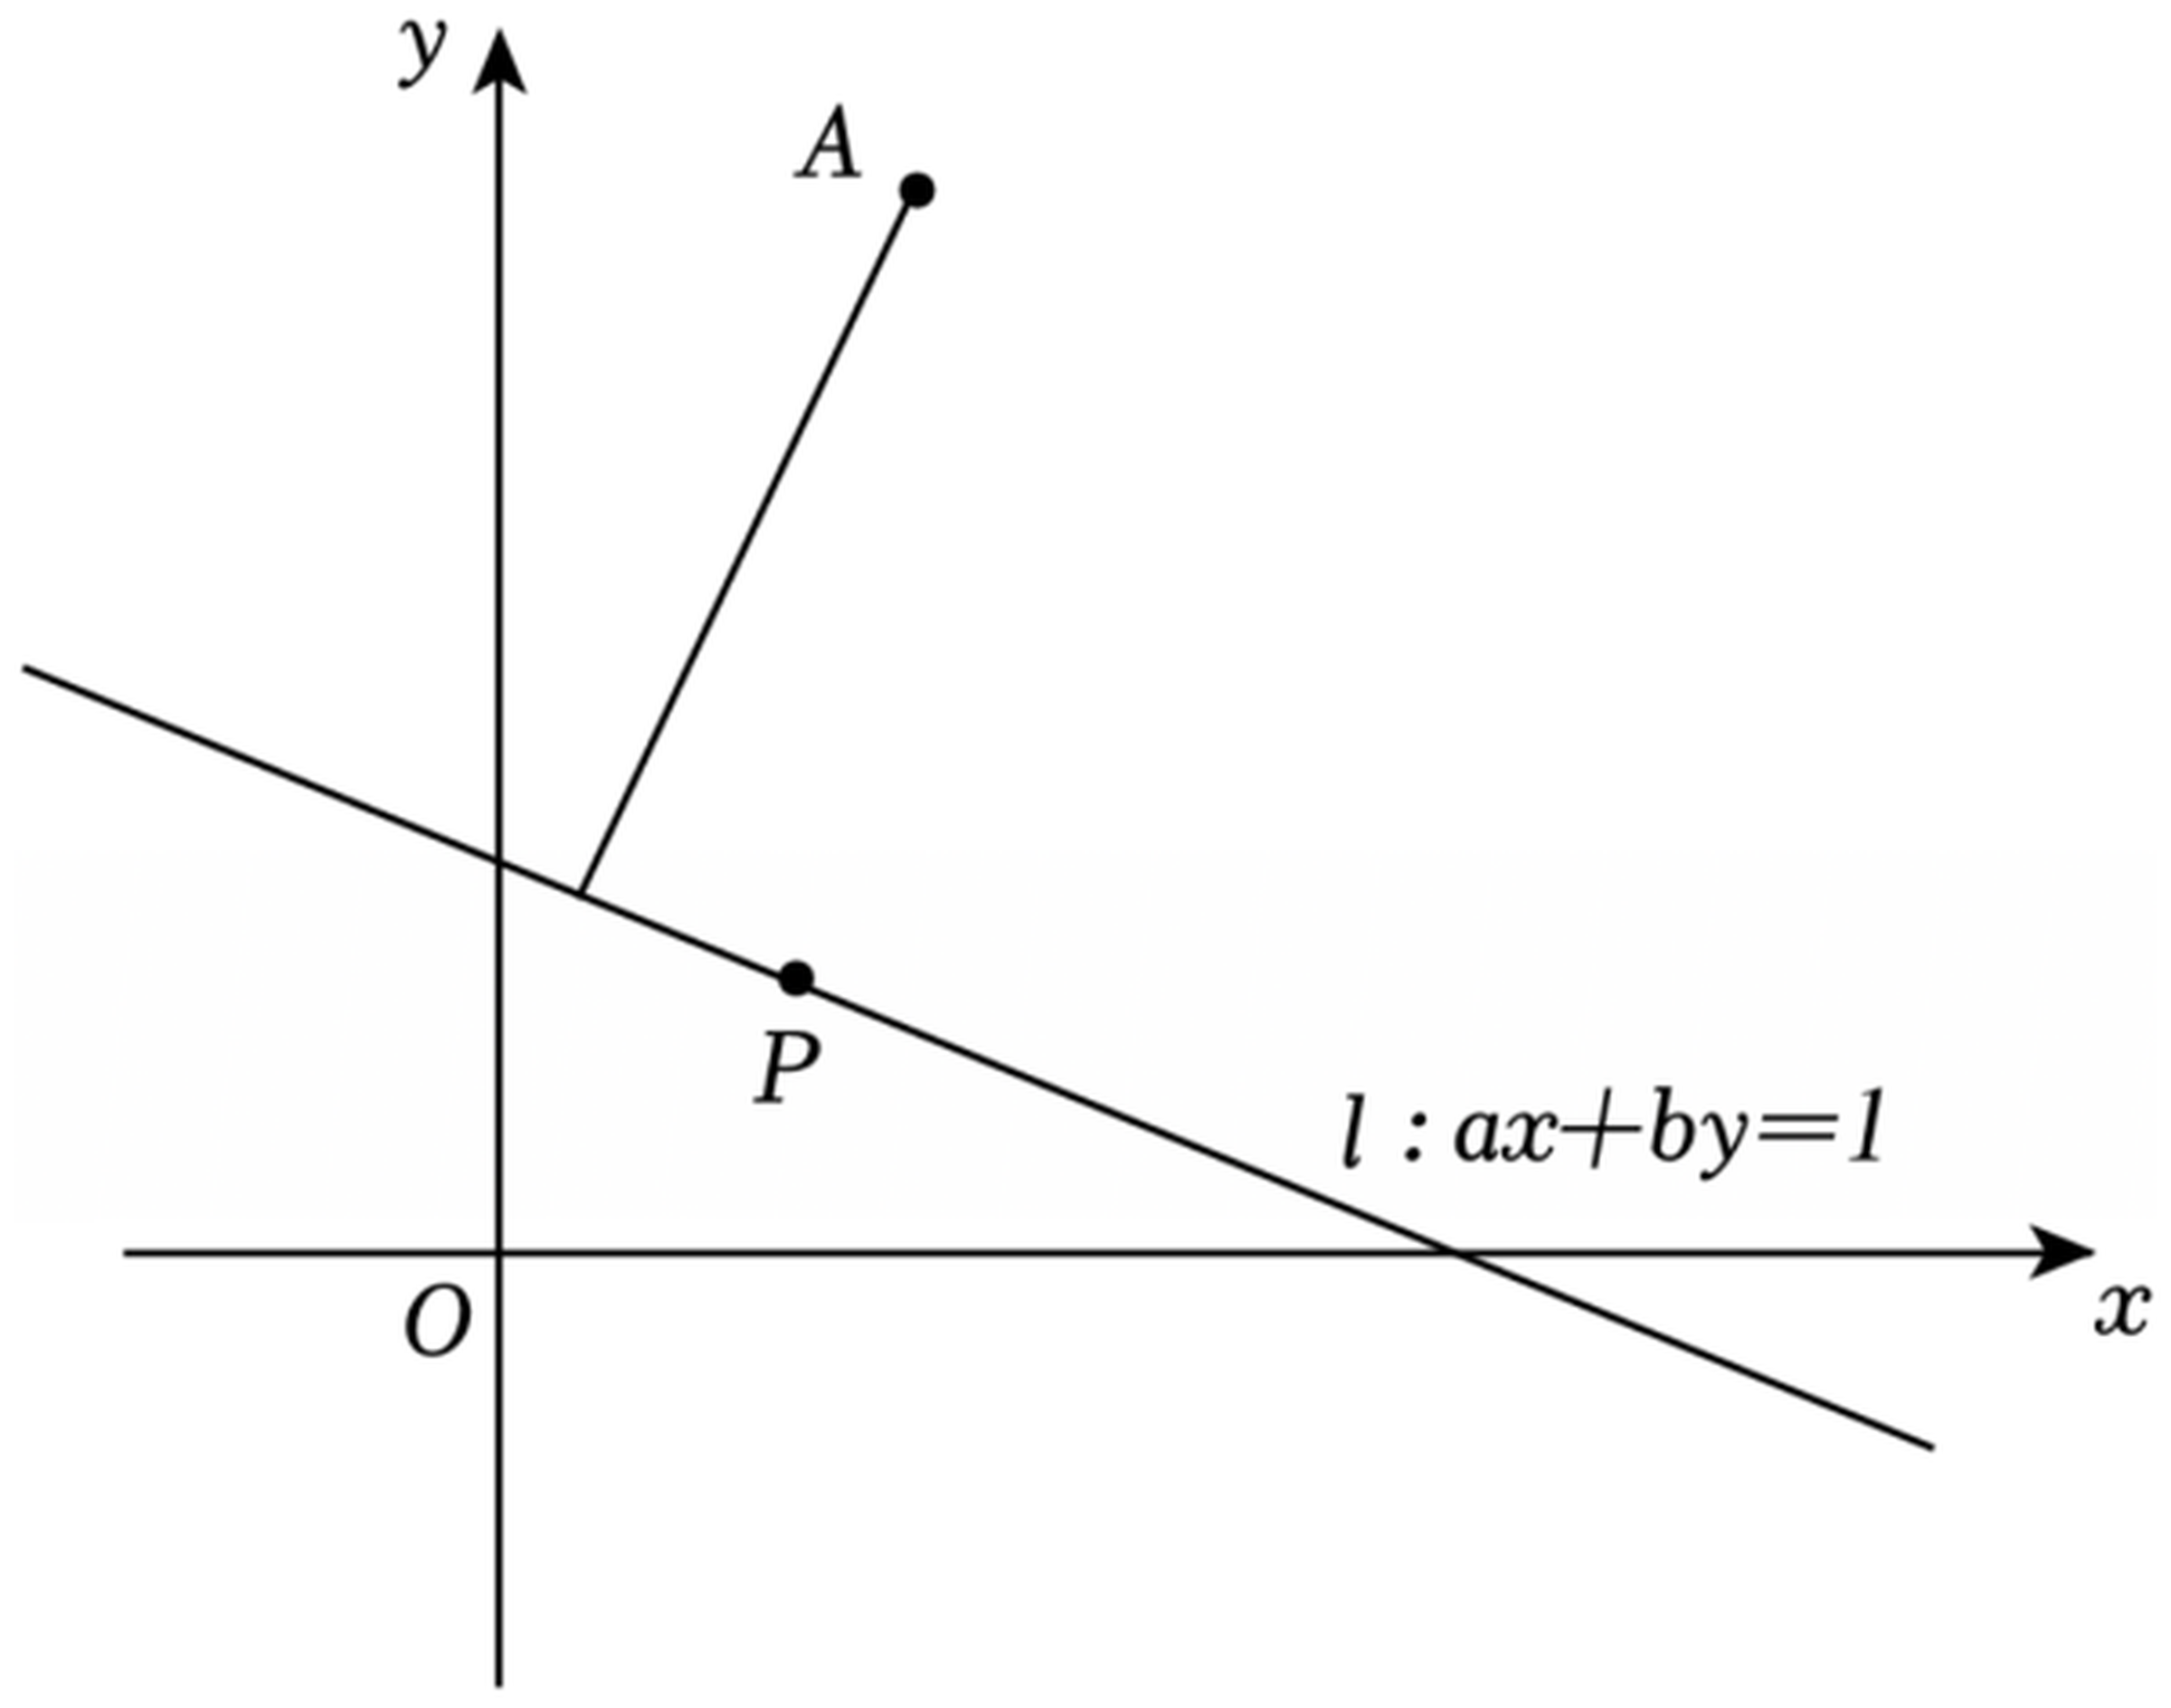
\includegraphics[width=0.56\textwidth]{figures/line_ax_plus_by_1.png}
\end{center}

\step{因为 $a+b=2$，所以直线 $l$ 恒过定点 $P\left(\dfrac12,\dfrac12\right)$，}
\step{再令 $A(1,2)$，则
$d_{A-l}=\dfrac{|a+2b-1|}{\sqrt{a^2+b^2}}\leqslant|AP|=\dfrac{\sqrt{10}}2$，}
\step{当且仅当 $l\perp AP$ 时等号成立，}
\step{又 $\dfrac{a+2b-1}{\sqrt{a^2+b^2}}\leqslant\dfrac{|a+2b-1|}{\sqrt{a^2+b^2}}$，
而当 $l\perp AP$，$a+2b-1>0$，等号也成立，}
\step{故 $\left(\dfrac{a+2b-1}{\sqrt{a^2+b^2}}\right)_{\max}=\dfrac{\sqrt{10}}2$.}
\solend

\fi

\ansspace[6]

\item （1）设 $a$、$b$、$c$ 都是正数，试证明不等式：
$\dfrac{b+c}a+\dfrac{c+a}b+\dfrac{a+b}c\geqslant6$；

（2）对一切正整数 $n$，不等式 $\dfrac{2x-1}x>\dfrac n{n+1}$ 恒成立，
则实数 $x$ 的取值范围构成的集合.

\ifanswer
\solbegin
\stepm{(1)}{因为 $a>0$，$b>0$，$c>0$，}
\step{所以 $\dfrac ba+\dfrac ab\geqslant2$，$\dfrac ca+\dfrac ac\geqslant2$，
$\dfrac cb+\dfrac bc\geqslant2$，}
\step{所以 $\left(\dfrac ba+\dfrac ab\right)+\left(\dfrac ca+\dfrac ac\right)
+\left(\dfrac cb+\dfrac bc\right)\geqslant6$，
即 $\dfrac{b+c}a+\dfrac{c+a}b+\dfrac{a+b}c\geqslant6$.}
% 注：下一行题干原卷作「……则实数 $x$ 的取值范围构成的集合.」，缺一个「求」字，
%     照抄未改，见文件头「原卷存疑」⑤。
\stepm{(2)}{考查 $y=\dfrac n{n+1}=1-\dfrac1{n+1}$，一切正整数 $n$ 函数为严格增函数，
所以 $y\geqslant\dfrac12$，}
\step{对一切正整数 $n$，不等式 $\dfrac{2x-1}x>\dfrac n{n+1}$ 恒成立，
所以 $\dfrac{2x-1}x\geqslant1$，}
\step{所以 $\dfrac{x-1}x\geqslant0$，所以 $x<0$ 或 $x\geqslant1$，}
\step{所以实数 $x$ 的取值范围是 $(-\infty,0)\cup[1,+\infty)$.}
\solend

\fi

\ansspace[6]

\end{enumerate}

\end{document}
"
% 紧凑版：xelatex "\def\iscompact{1}% 高一34_交附闵行_查漏补缺卷.tex
%   —— 高一上数学「2026-2027 年交附闵行高一上查漏补缺卷」（试卷版/答案版）
% 试卷版：xelatex 高一34_交附闵行_查漏补缺卷.tex
% 答案版：xelatex "\def\isanswer{1}\input{高一34_交附闵行_查漏补缺卷.tex}"
% 紧凑版：xelatex "\def\iscompact{1}\input{高一34_交附闵行_查漏补缺卷.tex}"
%
% 原始材料是微信公众号图文（公众号「魔都数学加油站」连载「27学年高一 34」，2026-09-25 发布，
% 原文标题「27学年高一34——2026-2027年上海市交附闵行高一上查漏补缺卷」），
% 正文为 7 张 PNG 页（均 2560×3620），取 mmbiz.qpic.cn/<hash>/0 的原图档。
% 原文本身就是一份**讲评版**，但**全卷没有任何一处印「【答案】」**——每题下方直接印【解析】，
% 答案写在解析的末句。试题文字与解析均照原卷录入，未改内容。
% 卷面的粉色斜水印属水印，未录入。
%
% 卷首标题：原卷印作「2026-2027 年交附闵行高一上查漏补缺卷」（公众号标题里的「上海市」
% 三字卷面标题行没有，本稿照卷面），年份区间按全稿惯例排 en dash，前缀照原卷保留「年」。
%
% 与原卷的排版差异（均已在 README「说明」中交代）：
%   ① 原文自**第 3 题**起（第 1、2 题未在该文中发布），故本稿题号亦自 3 起；
%   ② 原卷只有「一、填空题」「二、解答题」两个节标题（本卷无选择题），本稿照原卷分节，
%      只把标题改排成全稿统一的「大节标题」样式；
%   ③ 原卷通篇只印【解析】（无【答案】行），本稿统一改为试卷版隐去、答案版以 \ifanswer{}
%      块给出，两版彻底分离；
%   ④ 数集记号原卷两套并用：第 4 题与第 11(2) 题作斜体的 $R$，第 7 题两处作粗体的
%      $\mathbf{R}^+$，本稿按全稿惯例统一写作 $\R$；
%   ⑤ 原卷填空的横线约两个字宽，本稿按全稿惯例统一排 \blankline[4.4em]（第 9 题的第一个空
%      原卷**没有**下划线、只留了一个空格，本稿仍补出横线，见文件头「原卷存疑」①）；
%   ⑥ 原卷未印副标题，本稿按全稿惯例补出副标题「集合与常用逻辑用语」（本卷实为基本不等式
%      专题，与 高一27／高一28 同样只标主章节，见文末「高一34 专记」）；
%   ⑦ 第 13 题的配图只出现在【解析】里（题干并未写「如图」），故放进 \ifanswer 块，
%      试卷版不排；图取原卷截图、4× LANCZOS 放大（figures/line_ax_plus_by_1.png）。
%
% 原卷存疑五处（均照抄原卷、未改，见源码中该处上方注释）：
%   ① 第 9 题「则 $ab$ 的最大值为 ，」——第一个空后面只有空格、没有下划线，第二个空才有；
%   ② 第 11(2) 题题干括号内写「$a$、$b\in R$」，但函数式 $f(x)=ax^2+(3a-4)x-12$ 里并没有 $b$；
%   ③ 第 10 题只限定 $a$ 是正实数，未提 $b$ 的取值范围；
%   ④ 第 13 题题干作「求 …… 的最大值为____.」（「求」与「为」混用），且**题干未写「如图」**，
%      是【解析】里才写「如图」；
%   ⑤ 第 14(2) 题题干作「……则实数 $x$ 的取值范围构成的集合.」——缺一个「求」字。
% 另有两处标点照录：第 9 题【解析】首句末是句号、第 11(1)① 解析末句是分号。

\documentclass[a4paper,11pt]{article}
\usepackage{common}

\begin{document}

\examtitlest[3]{2026--2027 年交附闵行高一上查漏补缺卷}{集合与常用逻辑用语}

\bigsec{一、填空题}

\begin{enumerate}
\setcounter{enumi}{2}

\item 已知正实数 $m$、$n$ 满足 $\dfrac1{m+2n}+\dfrac1{2m+n}=1$，则 $m+n$ 的最小值为
\blankline[4.4em].

\ifanswer
\solbegin
\step{因为 $m$、$n\in(0,+\infty)$，$\dfrac1{m+2n}+\dfrac1{2m+n}=1$，}
\step{所以 $m+n=\dfrac13[(m+2n)+(2m+n)]\left(\dfrac1{m+2n}+\dfrac1{2m+n}\right)$}
\step{$=\dfrac13\left[2+\dfrac{2m+n}{m+2n}+\dfrac{m+2n}{2m+n}\right]
\geqslant\dfrac13\left[2+2\sqrt{\dfrac{2m+n}{m+2n}\cdot\dfrac{m+2n}{2m+n}}\right]
=\dfrac43$，}
\step{当且仅当 $\dfrac{2m+n}{m+2n}=\dfrac{m+2n}{2m+n}$，即 $m=n=\dfrac23$ 时取等号，}
\step{所以 $m+n$ 的最小值为 $\dfrac43$.}
\solend

\fi

\item 若 $a$、$b\in\R$，且 $a^2+2ab-3b^2=1$，则 $a^2+b^2$ 的最小值为 \blankline[4.4em].

\ifanswer
\solbegin
\step{由 $a^2+2ab-3b^2=1$ 得 $(a+3b)(a-b)=1$，}
\step{令 $x=a+3b$，$y=a-b$，则 $xy=1$ 且 $a=\dfrac{x+3y}4$，$b=\dfrac{x-y}4$，}
\step{所以 $a^2+b^2=\left(\dfrac{x+3y}4\right)^2+\left(\dfrac{x-y}4\right)^2
=\dfrac{x^2+5y^2+2}8\geqslant\dfrac{2\sqrt{5x^2y^2}+2}8=\dfrac{\sqrt5+1}4$，}
\step{当且仅当 $x^2=\sqrt5$，$y^2=\dfrac{\sqrt5}5$ 时取等号，
故 $a^2+b^2$ 的最小值为 $\dfrac{\sqrt5+1}4$.}
\solend

\fi

\item 已知实数 $x$、$y$ 满足 $3x^2+3y^2-2xy=4$，则 $x+y$ 的最大值为 \blankline[4.4em].

\ifanswer
\solbegin
\step{由 $3x^2+3y^2-2xy=4$，则 $3[(x+y)^2-2xy]-2xy=4$，}
\step{设 $s=x+y$，则 $3s^2-8xy=4$，即 $xy=\dfrac{3s^2-4}8$，}
\step{对任意实数 $x$、$y$，有 $xy\leqslant\left(\dfrac{x+y}2\right)^2=\dfrac{s^2}4$，
即 $\dfrac{3s^2-4}8\leqslant\dfrac{s^2}4$，}
\step{得 $s^2\leqslant4$，即 $-2\leqslant s\leqslant2$，}
\step{当 $x=y=1$ 时，满足原等式，且 $x+y=2$ 成立，因此 $x+y$ 的最大值为 $2$.}
\solend

\fi

\item 若 $a$、$b$、$c$ 都是正实数，则 $\dfrac{a^2+2b^2+4c^2}{ab+2bc}$ 的最小值为
\blankline[4.4em].

\ifanswer
\solbegin
\step{因为 $a^2+2b^2+4c^2=a^2+b^2+b^2+4c^2=(a^2+b^2)+(b^2+4c^2)\geqslant2ab+4bc$，}
\step{所以 $\dfrac{a^2+2b^2+4c^2}{ab+2bc}\geqslant\dfrac{2ab+4bc}{ab+2bc}=2$，
当且仅当 $a=b=2c$ 时取等号，}
\step{即 $\dfrac{a^2+2b^2+4c^2}{ab+2bc}$ 的最小值是 $2$.}
\solend

\fi

\item 已知 $a$、$b\in\R^+$，且 $ab=2$，则 $\dfrac b{2+a^2}+\dfrac a{2+b^2}$ 的最小值是
\blankline[4.4em].

\ifanswer
\solbegin
\step{$\dfrac b{2+a^2}+\dfrac a{2+b^2}=\dfrac b{ab+a^2}+\dfrac a{ab+b^2}
=\dfrac b{a(a+b)}+\dfrac a{b(a+b)}$}
\step{$=\dfrac{(a+b)^2-4}{2(a+b)}=\dfrac{a+b}2-\dfrac2{a+b}$，}
\step{令 $t=a+b$，则原式可设为 $y=\dfrac t2-\dfrac2t$ 的函数，}
\step{当 $t>0$ 时，此函数为严格增函数，}
\step{因为 $a$、$b\in\R^+$ 且 $ab=2$，$t=a+b\geqslant2\sqrt{ab}=2\sqrt2$，}
\step{当且仅当 $a=b=\sqrt2$ 时，$t$ 的最小值为 $2\sqrt2$，}
\step{$y=\dfrac t2-\dfrac2t$ 在 $t\in[2\sqrt2,+\infty)$ 上严格增，}
\step{所以原式的最小值为 $\dfrac{2\sqrt2}2-\dfrac2{2\sqrt2}=\dfrac{\sqrt2}2$，
则 $\dfrac b{2+a^2}+\dfrac a{2+b^2}$ 的最小值是 $\dfrac{\sqrt2}2$.}
\solend

\fi

\item 设 $x$、$y$、$z$ 为正实数，满足 $x-2y+3z=0$，则 $\dfrac{y^2}{xz}$ 的最小值是
\blankline[4.4em].

\ifanswer
\solbegin
\step{因为 $x-2y+3z=0$，所以 $y=\dfrac{x+3z}2$，}
\step{所以 $\dfrac{y^2}{xz}=\dfrac{x^2+9z^2+6xz}{4xz}\geqslant\dfrac{6xz+6xz}{4xz}=3$，
当且仅当 $x=3z$ 时取等号，}
\step{故 $\dfrac{y^2}{xz}$ 的最小值是 $3$.}
\solend

\fi

% 注：下一题的第一个空原卷只留了一个空格、**没有**下划线（第二个空才有），本稿仍按全稿
%     惯例补出横线；另其【解析】首句末原卷作句号，照录。见文件头「原卷存疑」①。
\item 设 $a$、$b$ 为正实数，且 $a+b=3$，则 $ab$ 的最大值为 \blankline[4.4em]，
$\dfrac{a^2}{a+2}+\dfrac{b^2}{b+1}$ 的最小值为 \blankline[4.4em].

\ifanswer
\solbegin
\step{因为 $a>0$，$b>0$，所以 $a+b=3\geqslant2\sqrt{ab}$，}
\step{故 $ab$ 的最大值为 $\dfrac94$，当且仅当 $a=b=\dfrac32$ 时取等号.}
\step{令 $a+2=m$，$b+1=n$，则 $m+n=a+b+3=6$，}
\step{解得 $a=m-2$，$b=n-1$，}
\step{所以 $\dfrac{a^2}{a+2}+\dfrac{b^2}{b+1}=\dfrac{(m-2)^2}m+\dfrac{(n-1)^2}n
=m+\dfrac4m+n+\dfrac1n-6=\dfrac4m+\dfrac1n$}
\step{$=\dfrac16(m+n)\left(\dfrac4m+\dfrac1n\right)
=\dfrac16\left(\dfrac{4n}m+\dfrac mn+5\right)\geqslant\dfrac16(4+5)=\dfrac32$，}
\step{当且仅当 $\dfrac{4n}m=\dfrac mn$ 时，即 $m=2n$ 时
$\dfrac{a^2}{a+2}+\dfrac{b^2}{b+1}$ 取得最小值，}
\step{因此 $\dfrac{a^2}{a+2}+\dfrac{b^2}{b+1}$ 的最小值为 $\dfrac32$.}
\solend

\fi

\item 若 $a$ 是正实数，$2a^2+3b^2=10$，则 $a\sqrt{2+b^2}$ 的最大值是 \blankline[4.4em].

\ifanswer
\solbegin
\step{$a$ 是正实数，$2a^2+3b^2=10$，变形为 $2a^2+3(b^2+2)=16$，}
\step{所以 $16\geqslant2\sqrt{2a^2\times3(b^2+2)}=2\sqrt6\cdot a\sqrt{b^2+2}$，
得 $a\sqrt{2+b^2}\leqslant\dfrac{4\sqrt6}3$，}
\step{当且仅当 $2a^2=3(b^2+2)=8$，即 $a=2$，$b^2=\dfrac23$ 时取等号，}
\step{所以 $a\sqrt{2+b^2}$ 的最大值为 $\dfrac{4\sqrt6}3$.}
\solend

\fi

\end{enumerate}

\bigsec{二、解答题}

\begin{enumerate}
\setcounter{enumi}{10}

\item （1）已知 $x>0$，$y>0$，$2xy=x+4y$. ①求 $xy$ 的最小值；②求 $x+y$ 的最小值.

（2）已知函数 $f(x)=ax^2+(3a-4)x-12$（$a$、$b\in\R$），求不等式 $f(x)\geqslant0$ 的解集.

\ifanswer
\solbegin
\stepm{(1)}{①因为 $x>0$，$y>0$，由基本不等式得
$2xy=x+4y\geqslant2\sqrt{4xy}=4\sqrt{xy}$，}
\step{解得 $xy\geqslant4$，当且仅当 $x=4y=4$ 时取等号，故 $xy$ 的最小值为 $4$；}
\step{②因为 $x>0$，$y>0$，由已知条件得 $\dfrac{4y+x}{xy}=\dfrac4x+\dfrac1y=2$，}
\step{所以 $x+y=\dfrac12(x+y)\left(\dfrac4x+\dfrac1y\right)
=\dfrac12\left(5+\dfrac{4y}x+\dfrac xy\right)
\geqslant\dfrac12\left(5+2\sqrt{\dfrac{4y}x\cdot\dfrac xy}\right)=\dfrac92$，}
\step{当且仅当 $x=2y=3$ 时，等号成立，故 $x+y$ 的最小值为 $\dfrac92$；}
% 注：下一行题干括号内原卷写「$a$、$b\in R$」，但函数式里并没有 $b$，照抄未改，
%     见文件头「原卷存疑」②。
\stepm{(2)}{当 $a=0$ 时，则 $x+3\leqslant0$，解得 $x\leqslant-3$；}
\step{当 $a\neq0$ 时，$f(x)=ax^2+(3a-4)x-12=(x+3)(ax-4)
=a(x+3)\left(x-\dfrac4a\right)$，}
\step{当 $a>0$ 时，则 $(x+3)\left(x-\dfrac4a\right)\geqslant0$，
解得 $x\leqslant-3$ 或 $x\geqslant\dfrac4a$；}
\step{当 $a<0$ 时，则 $(x+3)\left(x-\dfrac4a\right)\leqslant0$，}
\step{当 $\dfrac4a>-3$ 时，即 $a<-\dfrac43$，解 $(x+3)\left(x-\dfrac4a\right)\leqslant0$，
得 $-3\leqslant x\leqslant\dfrac4a$；}
\step{当 $\dfrac4a=-3$ 时，即 $a=-\dfrac43$，解 $(x+3)\left(x-\dfrac4a\right)\leqslant0$，
得 $x=-3$；}
\step{当 $\dfrac4a<-3$ 时，即 $-\dfrac43<a<0$，解 $(x+3)\left(x-\dfrac4a\right)\leqslant0$，
得 $\dfrac4a\leqslant x\leqslant-3$；}
\step{综上所述，当 $a<-\dfrac43$ 时，不等式 $f(x)\geqslant0$ 的解集为
$\left[-3,\dfrac4a\right]$；}
\step{当 $a=-\dfrac43$ 时，不等式 $f(x)\geqslant0$ 的解集为 $\{-3\}$；}
\step{当 $-\dfrac43<a<0$ 时，不等式 $f(x)\geqslant0$ 的解集为
$\left[\dfrac4a,-3\right]$；}
\step{当 $a=0$ 时，不等式 $f(x)\geqslant0$ 的解集为 $(-\infty,-3]$；}
\step{当 $a>0$ 时，不等式 $f(x)\geqslant0$ 的解集为
$(-\infty,-3]\cup\left[\dfrac4a,+\infty\right)$.}
\solend

\fi

\ansspace[8]

\item 已知 $x$、$y$ 都是正数，且 $\dfrac2x+\dfrac1y=1$.

\begin{enumerate}[label=(\arabic*)]
\item 求 $2x+y$ 的最小值及此时 $x$、$y$ 的取值；
\item 不等式 $(2x+y)^2\geqslant m(x+2y)$ 恒成立，求实数 $m$ 的取值范围.
\end{enumerate}

\ifanswer
\solbegin
\stepm{(1)}{$2x+y=(2x+y)\left(\dfrac2x+\dfrac1y\right)
=4+\dfrac{2x}y+\dfrac{2y}x+1\geqslant5+2\sqrt{\dfrac{2x}y\cdot\dfrac{2y}x}=9$，}
\step{当且仅当 $x=y$ 且 $\dfrac2x+\dfrac1y=1$，即 $x=y=3$ 时取等号，}
\step{此时 $2x+y$ 的最小值为 $9$.}
\stepm{(2)}{由 $\dfrac2x+\dfrac1y=1$，得 $x+2y=xy>0$，}
\step{故 $(2x+y)^2\geqslant m(x+2y)\Leftrightarrow m\leqslant\dfrac{(2x+y)^2}{x+2y}
\Leftrightarrow m\leqslant\dfrac{(2x+y)^2}{xy}$，}
\step{又 $\dfrac{(2x+y)^2}{xy}=\dfrac{4x^2+y^2+4xy}{xy}
=\dfrac{4x}y+\dfrac yx+4\geqslant2\sqrt{\dfrac{4x}y\cdot\dfrac yx}+4=8$，}
\step{当且仅当 $\begin{cases}\dfrac{4x}y=\dfrac yx\\[2pt]
\dfrac2x+\dfrac1y=1\end{cases}$ 时取等号，$\dfrac{(2x+y)^2}{xy}$ 取得最小值 $8$，}
\step{故 $m$ 的取值范围为 $\{m\mid m\leqslant8\}$.}
\solend

\fi

\ansspace[6]

% 注：本小题题干作「求 …… 的最大值为____.」（「求」与「为」混用），且**题干未写「如图」**
%     ——是【解析】里才写「如图」，照抄未改，见文件头「原卷存疑」④。
\item 已知实数 $a$、$b$ 满足 $a+b=2$，求 $\dfrac{a+2b-1}{\sqrt{a^2+b^2}}$ 的最大值为
\blankline[4.4em].

\ifanswer
\solbegin
\step{如图，考虑直线 $l:ax+by=1$，}

\begin{center}
% 图取原卷截图、4× LANCZOS 放大。图只在【解析】里出现（题干并未写「如图」），
% 故放进 \ifanswer 块，试卷版不排，见文件头⑦。
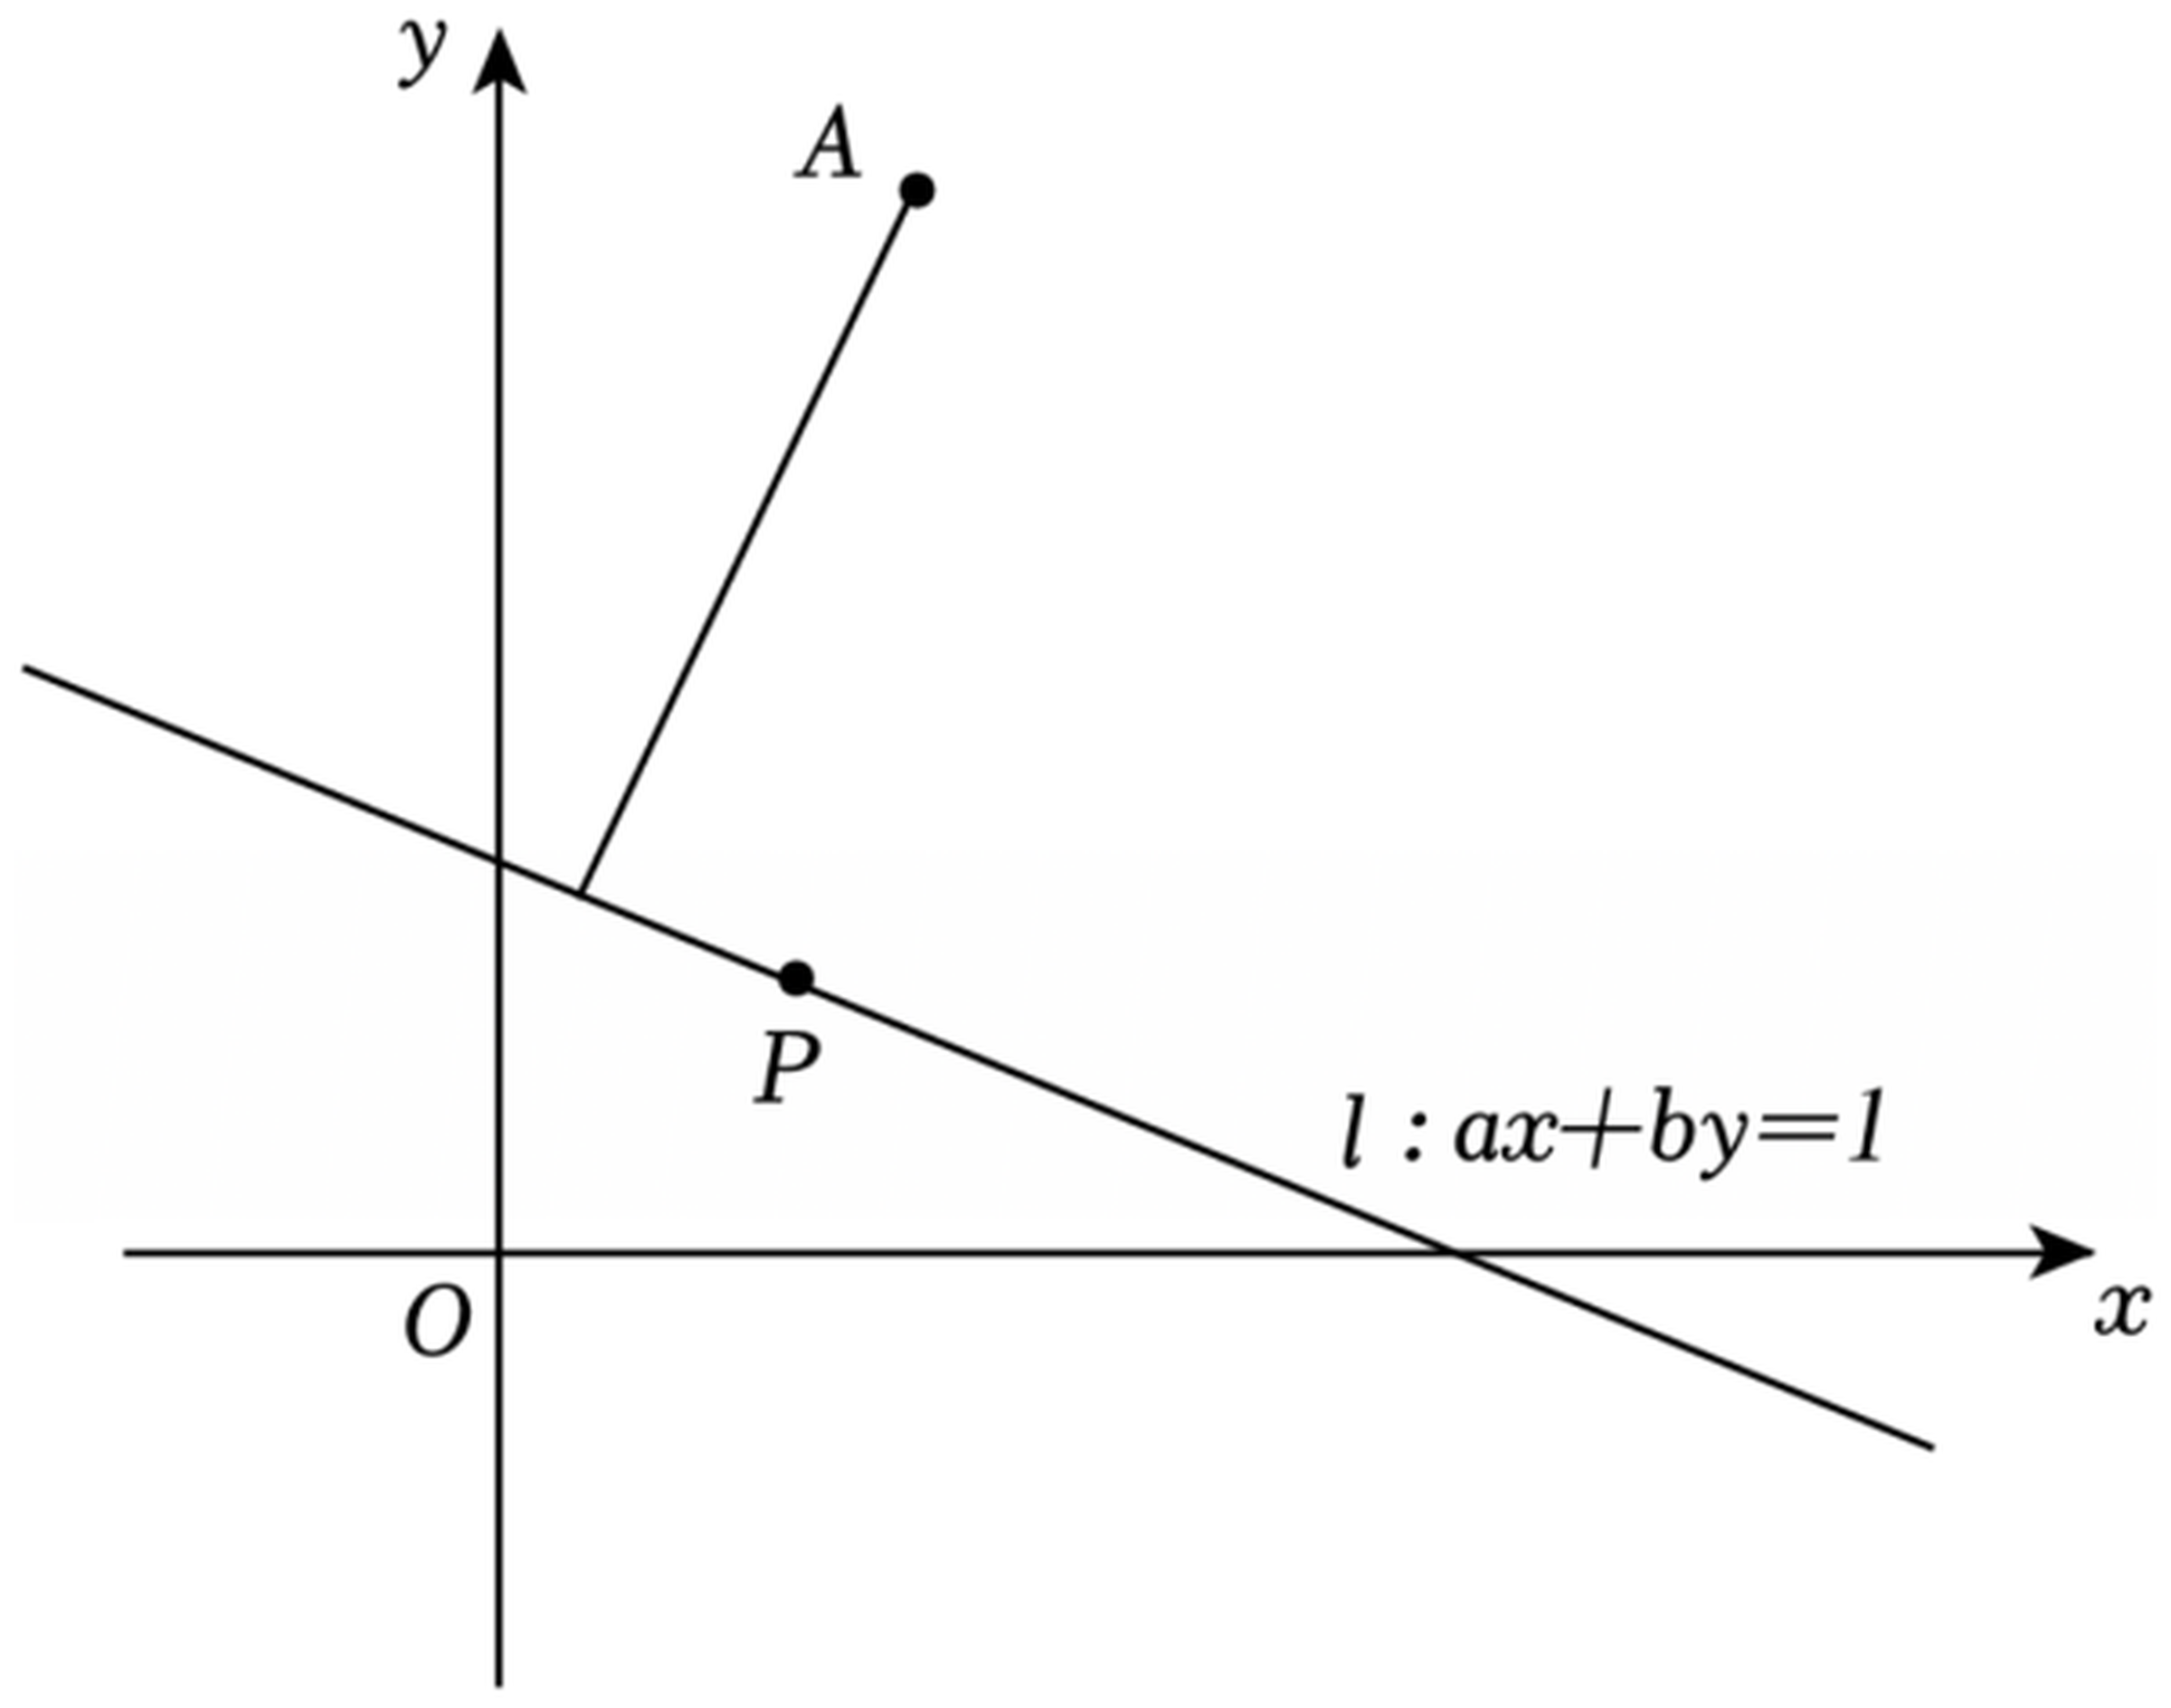
\includegraphics[width=0.56\textwidth]{figures/line_ax_plus_by_1.png}
\end{center}

\step{因为 $a+b=2$，所以直线 $l$ 恒过定点 $P\left(\dfrac12,\dfrac12\right)$，}
\step{再令 $A(1,2)$，则
$d_{A-l}=\dfrac{|a+2b-1|}{\sqrt{a^2+b^2}}\leqslant|AP|=\dfrac{\sqrt{10}}2$，}
\step{当且仅当 $l\perp AP$ 时等号成立，}
\step{又 $\dfrac{a+2b-1}{\sqrt{a^2+b^2}}\leqslant\dfrac{|a+2b-1|}{\sqrt{a^2+b^2}}$，
而当 $l\perp AP$，$a+2b-1>0$，等号也成立，}
\step{故 $\left(\dfrac{a+2b-1}{\sqrt{a^2+b^2}}\right)_{\max}=\dfrac{\sqrt{10}}2$.}
\solend

\fi

\ansspace[6]

\item （1）设 $a$、$b$、$c$ 都是正数，试证明不等式：
$\dfrac{b+c}a+\dfrac{c+a}b+\dfrac{a+b}c\geqslant6$；

（2）对一切正整数 $n$，不等式 $\dfrac{2x-1}x>\dfrac n{n+1}$ 恒成立，
则实数 $x$ 的取值范围构成的集合.

\ifanswer
\solbegin
\stepm{(1)}{因为 $a>0$，$b>0$，$c>0$，}
\step{所以 $\dfrac ba+\dfrac ab\geqslant2$，$\dfrac ca+\dfrac ac\geqslant2$，
$\dfrac cb+\dfrac bc\geqslant2$，}
\step{所以 $\left(\dfrac ba+\dfrac ab\right)+\left(\dfrac ca+\dfrac ac\right)
+\left(\dfrac cb+\dfrac bc\right)\geqslant6$，
即 $\dfrac{b+c}a+\dfrac{c+a}b+\dfrac{a+b}c\geqslant6$.}
% 注：下一行题干原卷作「……则实数 $x$ 的取值范围构成的集合.」，缺一个「求」字，
%     照抄未改，见文件头「原卷存疑」⑤。
\stepm{(2)}{考查 $y=\dfrac n{n+1}=1-\dfrac1{n+1}$，一切正整数 $n$ 函数为严格增函数，
所以 $y\geqslant\dfrac12$，}
\step{对一切正整数 $n$，不等式 $\dfrac{2x-1}x>\dfrac n{n+1}$ 恒成立，
所以 $\dfrac{2x-1}x\geqslant1$，}
\step{所以 $\dfrac{x-1}x\geqslant0$，所以 $x<0$ 或 $x\geqslant1$，}
\step{所以实数 $x$ 的取值范围是 $(-\infty,0)\cup[1,+\infty)$.}
\solend

\fi

\ansspace[6]

\end{enumerate}

\end{document}
"
%
% 原始材料是微信公众号图文（公众号「魔都数学加油站」连载「27学年高一 34」，2026-09-25 发布，
% 原文标题「27学年高一34——2026-2027年上海市交附闵行高一上查漏补缺卷」），
% 正文为 7 张 PNG 页（均 2560×3620），取 mmbiz.qpic.cn/<hash>/0 的原图档。
% 原文本身就是一份**讲评版**，但**全卷没有任何一处印「【答案】」**——每题下方直接印【解析】，
% 答案写在解析的末句。试题文字与解析均照原卷录入，未改内容。
% 卷面的粉色斜水印属水印，未录入。
%
% 卷首标题：原卷印作「2026-2027 年交附闵行高一上查漏补缺卷」（公众号标题里的「上海市」
% 三字卷面标题行没有，本稿照卷面），年份区间按全稿惯例排 en dash，前缀照原卷保留「年」。
%
% 与原卷的排版差异（均已在 README「说明」中交代）：
%   ① 原文自**第 3 题**起（第 1、2 题未在该文中发布），故本稿题号亦自 3 起；
%   ② 原卷只有「一、填空题」「二、解答题」两个节标题（本卷无选择题），本稿照原卷分节，
%      只把标题改排成全稿统一的「大节标题」样式；
%   ③ 原卷通篇只印【解析】（无【答案】行），本稿统一改为试卷版隐去、答案版以 \ifanswer{}
%      块给出，两版彻底分离；
%   ④ 数集记号原卷两套并用：第 4 题与第 11(2) 题作斜体的 $R$，第 7 题两处作粗体的
%      $\mathbf{R}^+$，本稿按全稿惯例统一写作 $\R$；
%   ⑤ 原卷填空的横线约两个字宽，本稿按全稿惯例统一排 \blankline[4.4em]（第 9 题的第一个空
%      原卷**没有**下划线、只留了一个空格，本稿仍补出横线，见文件头「原卷存疑」①）；
%   ⑥ 原卷未印副标题，本稿按全稿惯例补出副标题「集合与常用逻辑用语」（本卷实为基本不等式
%      专题，与 高一27／高一28 同样只标主章节，见文末「高一34 专记」）；
%   ⑦ 第 13 题的配图只出现在【解析】里（题干并未写「如图」），故放进 \ifanswer 块，
%      试卷版不排；图取原卷截图、4× LANCZOS 放大（figures/line_ax_plus_by_1.png）。
%
% 原卷存疑五处（均照抄原卷、未改，见源码中该处上方注释）：
%   ① 第 9 题「则 $ab$ 的最大值为 ，」——第一个空后面只有空格、没有下划线，第二个空才有；
%   ② 第 11(2) 题题干括号内写「$a$、$b\in R$」，但函数式 $f(x)=ax^2+(3a-4)x-12$ 里并没有 $b$；
%   ③ 第 10 题只限定 $a$ 是正实数，未提 $b$ 的取值范围；
%   ④ 第 13 题题干作「求 …… 的最大值为____.」（「求」与「为」混用），且**题干未写「如图」**，
%      是【解析】里才写「如图」；
%   ⑤ 第 14(2) 题题干作「……则实数 $x$ 的取值范围构成的集合.」——缺一个「求」字。
% 另有两处标点照录：第 9 题【解析】首句末是句号、第 11(1)① 解析末句是分号。

\documentclass[a4paper,11pt]{article}
\usepackage{common}

\begin{document}

\examtitlest[3]{2026--2027 年交附闵行高一上查漏补缺卷}{集合与常用逻辑用语}

\bigsec{一、填空题}

\begin{enumerate}
\setcounter{enumi}{2}

\item 已知正实数 $m$、$n$ 满足 $\dfrac1{m+2n}+\dfrac1{2m+n}=1$，则 $m+n$ 的最小值为
\blankline[4.4em].

\ifanswer
\solbegin
\step{因为 $m$、$n\in(0,+\infty)$，$\dfrac1{m+2n}+\dfrac1{2m+n}=1$，}
\step{所以 $m+n=\dfrac13[(m+2n)+(2m+n)]\left(\dfrac1{m+2n}+\dfrac1{2m+n}\right)$}
\step{$=\dfrac13\left[2+\dfrac{2m+n}{m+2n}+\dfrac{m+2n}{2m+n}\right]
\geqslant\dfrac13\left[2+2\sqrt{\dfrac{2m+n}{m+2n}\cdot\dfrac{m+2n}{2m+n}}\right]
=\dfrac43$，}
\step{当且仅当 $\dfrac{2m+n}{m+2n}=\dfrac{m+2n}{2m+n}$，即 $m=n=\dfrac23$ 时取等号，}
\step{所以 $m+n$ 的最小值为 $\dfrac43$.}
\solend

\fi

\item 若 $a$、$b\in\R$，且 $a^2+2ab-3b^2=1$，则 $a^2+b^2$ 的最小值为 \blankline[4.4em].

\ifanswer
\solbegin
\step{由 $a^2+2ab-3b^2=1$ 得 $(a+3b)(a-b)=1$，}
\step{令 $x=a+3b$，$y=a-b$，则 $xy=1$ 且 $a=\dfrac{x+3y}4$，$b=\dfrac{x-y}4$，}
\step{所以 $a^2+b^2=\left(\dfrac{x+3y}4\right)^2+\left(\dfrac{x-y}4\right)^2
=\dfrac{x^2+5y^2+2}8\geqslant\dfrac{2\sqrt{5x^2y^2}+2}8=\dfrac{\sqrt5+1}4$，}
\step{当且仅当 $x^2=\sqrt5$，$y^2=\dfrac{\sqrt5}5$ 时取等号，
故 $a^2+b^2$ 的最小值为 $\dfrac{\sqrt5+1}4$.}
\solend

\fi

\item 已知实数 $x$、$y$ 满足 $3x^2+3y^2-2xy=4$，则 $x+y$ 的最大值为 \blankline[4.4em].

\ifanswer
\solbegin
\step{由 $3x^2+3y^2-2xy=4$，则 $3[(x+y)^2-2xy]-2xy=4$，}
\step{设 $s=x+y$，则 $3s^2-8xy=4$，即 $xy=\dfrac{3s^2-4}8$，}
\step{对任意实数 $x$、$y$，有 $xy\leqslant\left(\dfrac{x+y}2\right)^2=\dfrac{s^2}4$，
即 $\dfrac{3s^2-4}8\leqslant\dfrac{s^2}4$，}
\step{得 $s^2\leqslant4$，即 $-2\leqslant s\leqslant2$，}
\step{当 $x=y=1$ 时，满足原等式，且 $x+y=2$ 成立，因此 $x+y$ 的最大值为 $2$.}
\solend

\fi

\item 若 $a$、$b$、$c$ 都是正实数，则 $\dfrac{a^2+2b^2+4c^2}{ab+2bc}$ 的最小值为
\blankline[4.4em].

\ifanswer
\solbegin
\step{因为 $a^2+2b^2+4c^2=a^2+b^2+b^2+4c^2=(a^2+b^2)+(b^2+4c^2)\geqslant2ab+4bc$，}
\step{所以 $\dfrac{a^2+2b^2+4c^2}{ab+2bc}\geqslant\dfrac{2ab+4bc}{ab+2bc}=2$，
当且仅当 $a=b=2c$ 时取等号，}
\step{即 $\dfrac{a^2+2b^2+4c^2}{ab+2bc}$ 的最小值是 $2$.}
\solend

\fi

\item 已知 $a$、$b\in\R^+$，且 $ab=2$，则 $\dfrac b{2+a^2}+\dfrac a{2+b^2}$ 的最小值是
\blankline[4.4em].

\ifanswer
\solbegin
\step{$\dfrac b{2+a^2}+\dfrac a{2+b^2}=\dfrac b{ab+a^2}+\dfrac a{ab+b^2}
=\dfrac b{a(a+b)}+\dfrac a{b(a+b)}$}
\step{$=\dfrac{(a+b)^2-4}{2(a+b)}=\dfrac{a+b}2-\dfrac2{a+b}$，}
\step{令 $t=a+b$，则原式可设为 $y=\dfrac t2-\dfrac2t$ 的函数，}
\step{当 $t>0$ 时，此函数为严格增函数，}
\step{因为 $a$、$b\in\R^+$ 且 $ab=2$，$t=a+b\geqslant2\sqrt{ab}=2\sqrt2$，}
\step{当且仅当 $a=b=\sqrt2$ 时，$t$ 的最小值为 $2\sqrt2$，}
\step{$y=\dfrac t2-\dfrac2t$ 在 $t\in[2\sqrt2,+\infty)$ 上严格增，}
\step{所以原式的最小值为 $\dfrac{2\sqrt2}2-\dfrac2{2\sqrt2}=\dfrac{\sqrt2}2$，
则 $\dfrac b{2+a^2}+\dfrac a{2+b^2}$ 的最小值是 $\dfrac{\sqrt2}2$.}
\solend

\fi

\item 设 $x$、$y$、$z$ 为正实数，满足 $x-2y+3z=0$，则 $\dfrac{y^2}{xz}$ 的最小值是
\blankline[4.4em].

\ifanswer
\solbegin
\step{因为 $x-2y+3z=0$，所以 $y=\dfrac{x+3z}2$，}
\step{所以 $\dfrac{y^2}{xz}=\dfrac{x^2+9z^2+6xz}{4xz}\geqslant\dfrac{6xz+6xz}{4xz}=3$，
当且仅当 $x=3z$ 时取等号，}
\step{故 $\dfrac{y^2}{xz}$ 的最小值是 $3$.}
\solend

\fi

% 注：下一题的第一个空原卷只留了一个空格、**没有**下划线（第二个空才有），本稿仍按全稿
%     惯例补出横线；另其【解析】首句末原卷作句号，照录。见文件头「原卷存疑」①。
\item 设 $a$、$b$ 为正实数，且 $a+b=3$，则 $ab$ 的最大值为 \blankline[4.4em]，
$\dfrac{a^2}{a+2}+\dfrac{b^2}{b+1}$ 的最小值为 \blankline[4.4em].

\ifanswer
\solbegin
\step{因为 $a>0$，$b>0$，所以 $a+b=3\geqslant2\sqrt{ab}$，}
\step{故 $ab$ 的最大值为 $\dfrac94$，当且仅当 $a=b=\dfrac32$ 时取等号.}
\step{令 $a+2=m$，$b+1=n$，则 $m+n=a+b+3=6$，}
\step{解得 $a=m-2$，$b=n-1$，}
\step{所以 $\dfrac{a^2}{a+2}+\dfrac{b^2}{b+1}=\dfrac{(m-2)^2}m+\dfrac{(n-1)^2}n
=m+\dfrac4m+n+\dfrac1n-6=\dfrac4m+\dfrac1n$}
\step{$=\dfrac16(m+n)\left(\dfrac4m+\dfrac1n\right)
=\dfrac16\left(\dfrac{4n}m+\dfrac mn+5\right)\geqslant\dfrac16(4+5)=\dfrac32$，}
\step{当且仅当 $\dfrac{4n}m=\dfrac mn$ 时，即 $m=2n$ 时
$\dfrac{a^2}{a+2}+\dfrac{b^2}{b+1}$ 取得最小值，}
\step{因此 $\dfrac{a^2}{a+2}+\dfrac{b^2}{b+1}$ 的最小值为 $\dfrac32$.}
\solend

\fi

\item 若 $a$ 是正实数，$2a^2+3b^2=10$，则 $a\sqrt{2+b^2}$ 的最大值是 \blankline[4.4em].

\ifanswer
\solbegin
\step{$a$ 是正实数，$2a^2+3b^2=10$，变形为 $2a^2+3(b^2+2)=16$，}
\step{所以 $16\geqslant2\sqrt{2a^2\times3(b^2+2)}=2\sqrt6\cdot a\sqrt{b^2+2}$，
得 $a\sqrt{2+b^2}\leqslant\dfrac{4\sqrt6}3$，}
\step{当且仅当 $2a^2=3(b^2+2)=8$，即 $a=2$，$b^2=\dfrac23$ 时取等号，}
\step{所以 $a\sqrt{2+b^2}$ 的最大值为 $\dfrac{4\sqrt6}3$.}
\solend

\fi

\end{enumerate}

\bigsec{二、解答题}

\begin{enumerate}
\setcounter{enumi}{10}

\item （1）已知 $x>0$，$y>0$，$2xy=x+4y$. ①求 $xy$ 的最小值；②求 $x+y$ 的最小值.

（2）已知函数 $f(x)=ax^2+(3a-4)x-12$（$a$、$b\in\R$），求不等式 $f(x)\geqslant0$ 的解集.

\ifanswer
\solbegin
\stepm{(1)}{①因为 $x>0$，$y>0$，由基本不等式得
$2xy=x+4y\geqslant2\sqrt{4xy}=4\sqrt{xy}$，}
\step{解得 $xy\geqslant4$，当且仅当 $x=4y=4$ 时取等号，故 $xy$ 的最小值为 $4$；}
\step{②因为 $x>0$，$y>0$，由已知条件得 $\dfrac{4y+x}{xy}=\dfrac4x+\dfrac1y=2$，}
\step{所以 $x+y=\dfrac12(x+y)\left(\dfrac4x+\dfrac1y\right)
=\dfrac12\left(5+\dfrac{4y}x+\dfrac xy\right)
\geqslant\dfrac12\left(5+2\sqrt{\dfrac{4y}x\cdot\dfrac xy}\right)=\dfrac92$，}
\step{当且仅当 $x=2y=3$ 时，等号成立，故 $x+y$ 的最小值为 $\dfrac92$；}
% 注：下一行题干括号内原卷写「$a$、$b\in R$」，但函数式里并没有 $b$，照抄未改，
%     见文件头「原卷存疑」②。
\stepm{(2)}{当 $a=0$ 时，则 $x+3\leqslant0$，解得 $x\leqslant-3$；}
\step{当 $a\neq0$ 时，$f(x)=ax^2+(3a-4)x-12=(x+3)(ax-4)
=a(x+3)\left(x-\dfrac4a\right)$，}
\step{当 $a>0$ 时，则 $(x+3)\left(x-\dfrac4a\right)\geqslant0$，
解得 $x\leqslant-3$ 或 $x\geqslant\dfrac4a$；}
\step{当 $a<0$ 时，则 $(x+3)\left(x-\dfrac4a\right)\leqslant0$，}
\step{当 $\dfrac4a>-3$ 时，即 $a<-\dfrac43$，解 $(x+3)\left(x-\dfrac4a\right)\leqslant0$，
得 $-3\leqslant x\leqslant\dfrac4a$；}
\step{当 $\dfrac4a=-3$ 时，即 $a=-\dfrac43$，解 $(x+3)\left(x-\dfrac4a\right)\leqslant0$，
得 $x=-3$；}
\step{当 $\dfrac4a<-3$ 时，即 $-\dfrac43<a<0$，解 $(x+3)\left(x-\dfrac4a\right)\leqslant0$，
得 $\dfrac4a\leqslant x\leqslant-3$；}
\step{综上所述，当 $a<-\dfrac43$ 时，不等式 $f(x)\geqslant0$ 的解集为
$\left[-3,\dfrac4a\right]$；}
\step{当 $a=-\dfrac43$ 时，不等式 $f(x)\geqslant0$ 的解集为 $\{-3\}$；}
\step{当 $-\dfrac43<a<0$ 时，不等式 $f(x)\geqslant0$ 的解集为
$\left[\dfrac4a,-3\right]$；}
\step{当 $a=0$ 时，不等式 $f(x)\geqslant0$ 的解集为 $(-\infty,-3]$；}
\step{当 $a>0$ 时，不等式 $f(x)\geqslant0$ 的解集为
$(-\infty,-3]\cup\left[\dfrac4a,+\infty\right)$.}
\solend

\fi

\ansspace[8]

\item 已知 $x$、$y$ 都是正数，且 $\dfrac2x+\dfrac1y=1$.

\begin{enumerate}[label=(\arabic*)]
\item 求 $2x+y$ 的最小值及此时 $x$、$y$ 的取值；
\item 不等式 $(2x+y)^2\geqslant m(x+2y)$ 恒成立，求实数 $m$ 的取值范围.
\end{enumerate}

\ifanswer
\solbegin
\stepm{(1)}{$2x+y=(2x+y)\left(\dfrac2x+\dfrac1y\right)
=4+\dfrac{2x}y+\dfrac{2y}x+1\geqslant5+2\sqrt{\dfrac{2x}y\cdot\dfrac{2y}x}=9$，}
\step{当且仅当 $x=y$ 且 $\dfrac2x+\dfrac1y=1$，即 $x=y=3$ 时取等号，}
\step{此时 $2x+y$ 的最小值为 $9$.}
\stepm{(2)}{由 $\dfrac2x+\dfrac1y=1$，得 $x+2y=xy>0$，}
\step{故 $(2x+y)^2\geqslant m(x+2y)\Leftrightarrow m\leqslant\dfrac{(2x+y)^2}{x+2y}
\Leftrightarrow m\leqslant\dfrac{(2x+y)^2}{xy}$，}
\step{又 $\dfrac{(2x+y)^2}{xy}=\dfrac{4x^2+y^2+4xy}{xy}
=\dfrac{4x}y+\dfrac yx+4\geqslant2\sqrt{\dfrac{4x}y\cdot\dfrac yx}+4=8$，}
\step{当且仅当 $\begin{cases}\dfrac{4x}y=\dfrac yx\\[2pt]
\dfrac2x+\dfrac1y=1\end{cases}$ 时取等号，$\dfrac{(2x+y)^2}{xy}$ 取得最小值 $8$，}
\step{故 $m$ 的取值范围为 $\{m\mid m\leqslant8\}$.}
\solend

\fi

\ansspace[6]

% 注：本小题题干作「求 …… 的最大值为____.」（「求」与「为」混用），且**题干未写「如图」**
%     ——是【解析】里才写「如图」，照抄未改，见文件头「原卷存疑」④。
\item 已知实数 $a$、$b$ 满足 $a+b=2$，求 $\dfrac{a+2b-1}{\sqrt{a^2+b^2}}$ 的最大值为
\blankline[4.4em].

\ifanswer
\solbegin
\step{如图，考虑直线 $l:ax+by=1$，}

\begin{center}
% 图取原卷截图、4× LANCZOS 放大。图只在【解析】里出现（题干并未写「如图」），
% 故放进 \ifanswer 块，试卷版不排，见文件头⑦。
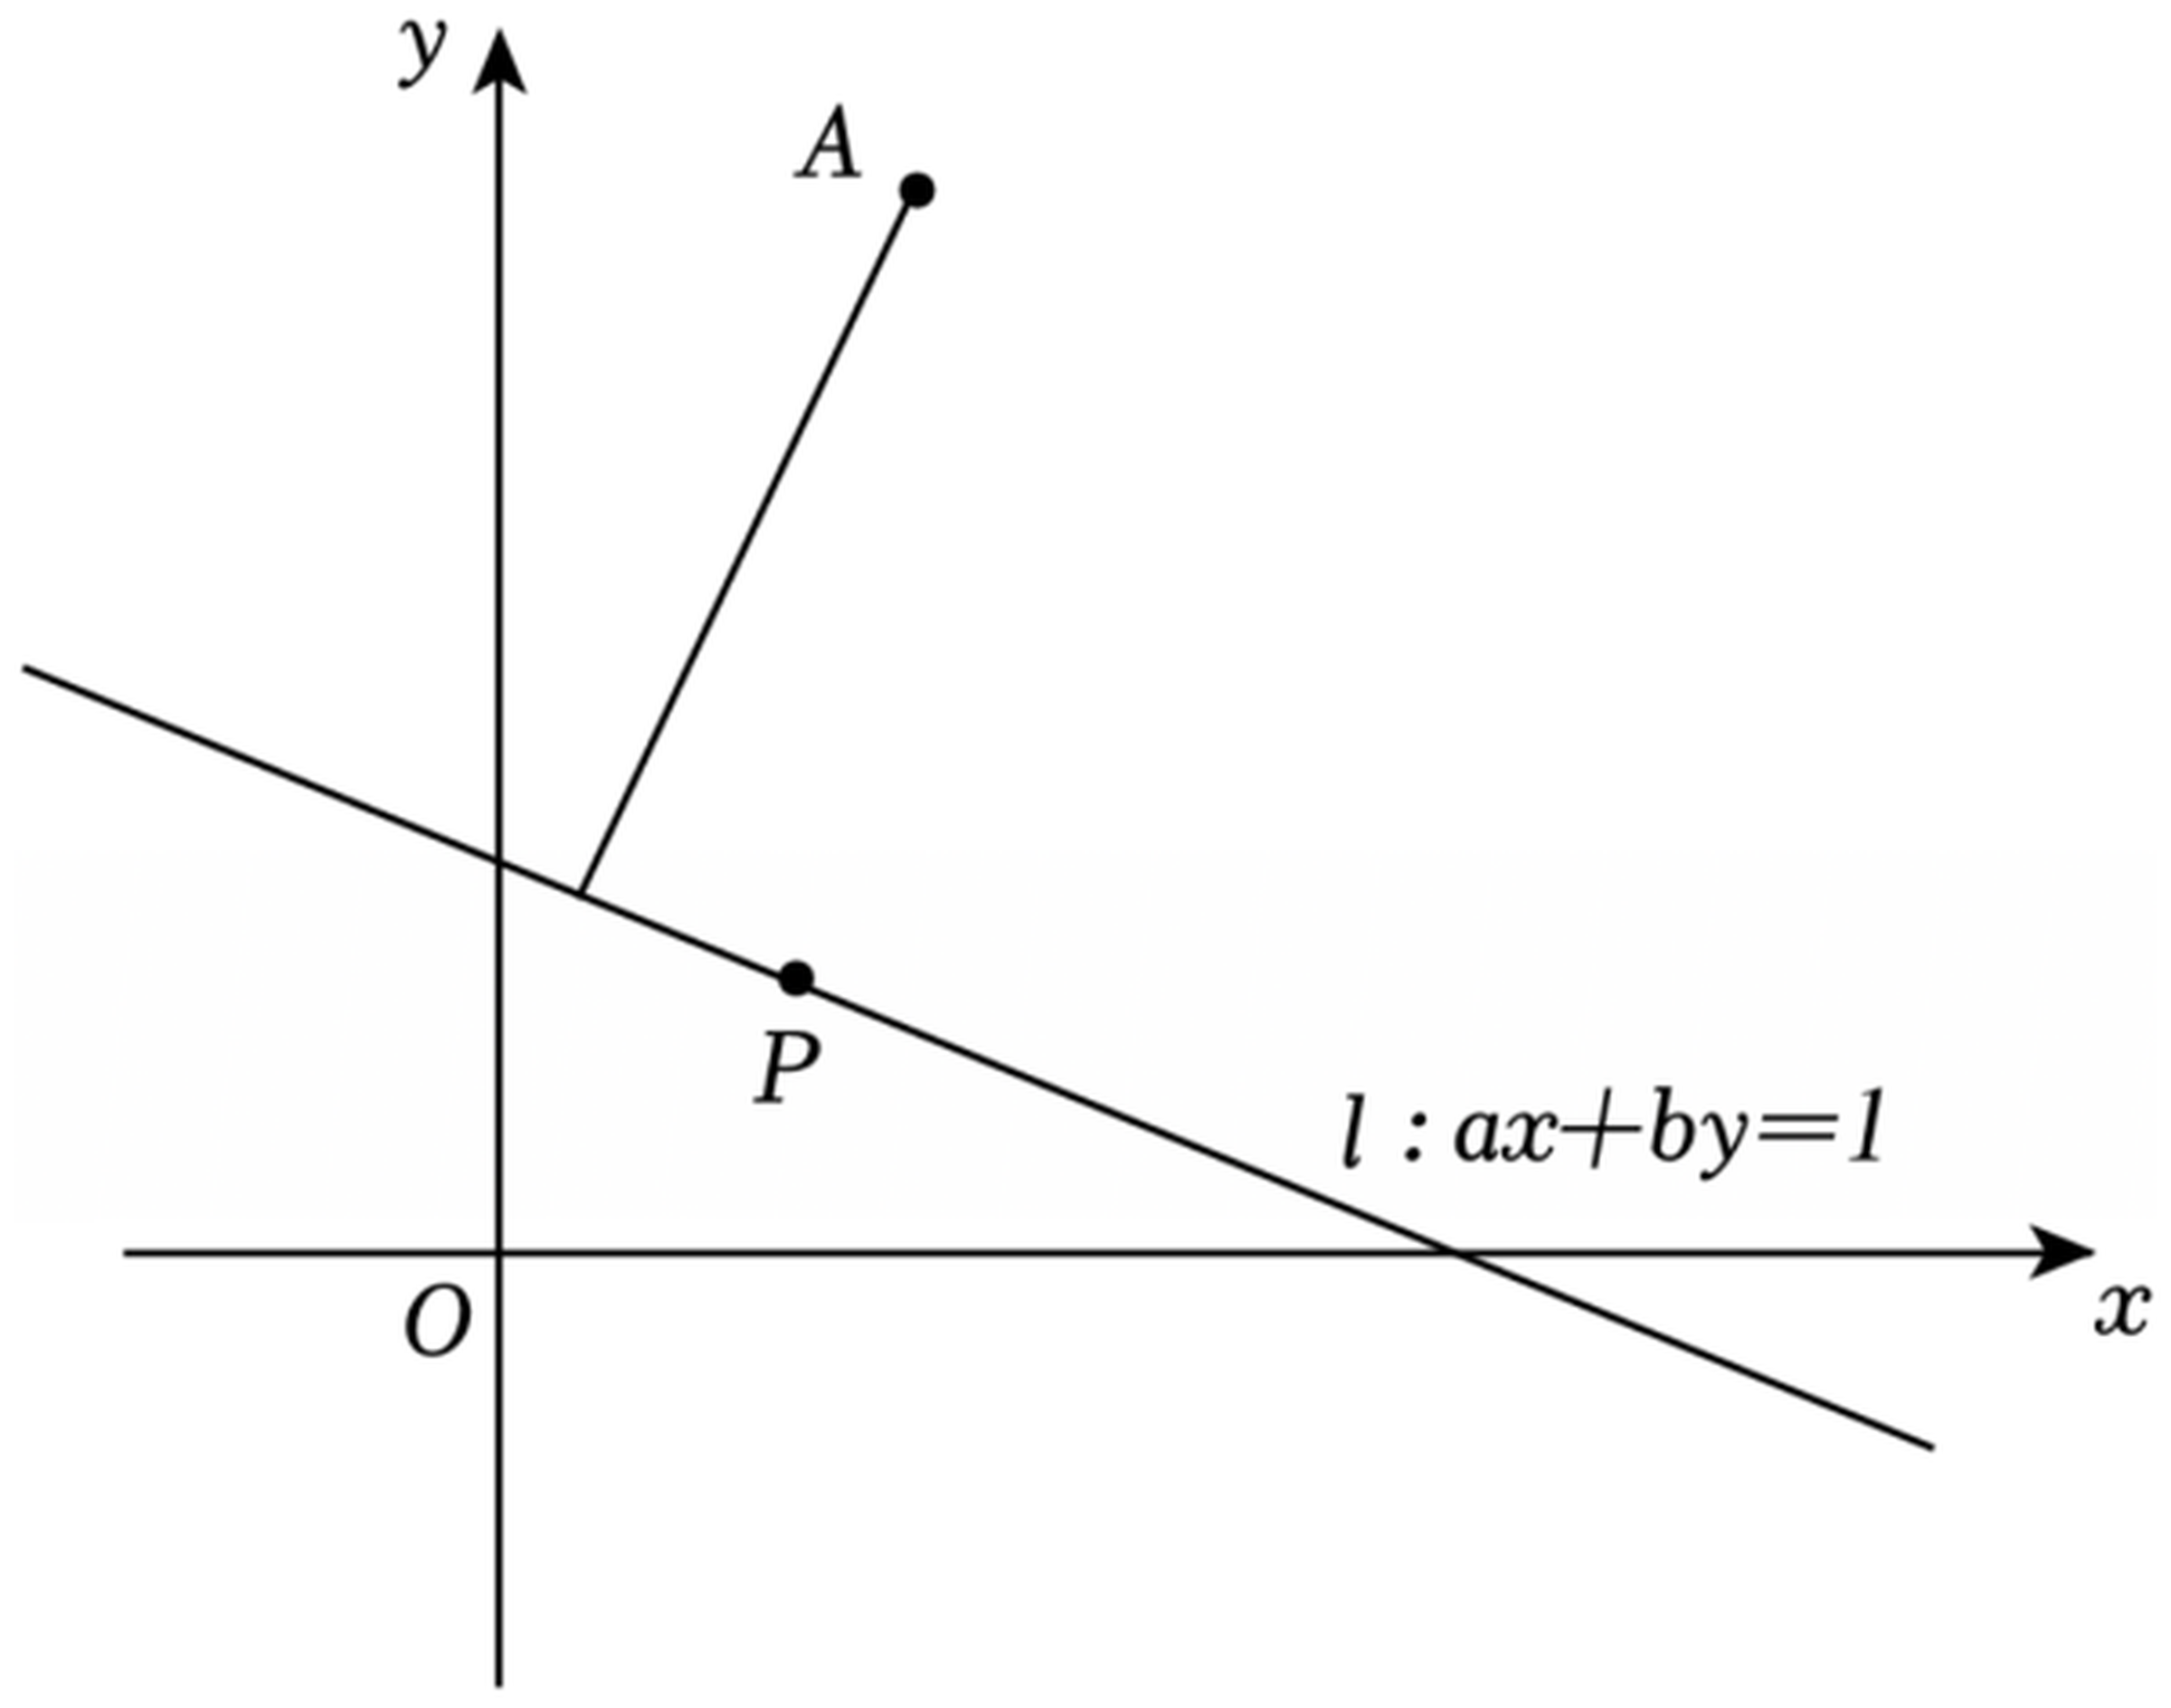
\includegraphics[width=0.56\textwidth]{figures/line_ax_plus_by_1.png}
\end{center}

\step{因为 $a+b=2$，所以直线 $l$ 恒过定点 $P\left(\dfrac12,\dfrac12\right)$，}
\step{再令 $A(1,2)$，则
$d_{A-l}=\dfrac{|a+2b-1|}{\sqrt{a^2+b^2}}\leqslant|AP|=\dfrac{\sqrt{10}}2$，}
\step{当且仅当 $l\perp AP$ 时等号成立，}
\step{又 $\dfrac{a+2b-1}{\sqrt{a^2+b^2}}\leqslant\dfrac{|a+2b-1|}{\sqrt{a^2+b^2}}$，
而当 $l\perp AP$，$a+2b-1>0$，等号也成立，}
\step{故 $\left(\dfrac{a+2b-1}{\sqrt{a^2+b^2}}\right)_{\max}=\dfrac{\sqrt{10}}2$.}
\solend

\fi

\ansspace[6]

\item （1）设 $a$、$b$、$c$ 都是正数，试证明不等式：
$\dfrac{b+c}a+\dfrac{c+a}b+\dfrac{a+b}c\geqslant6$；

（2）对一切正整数 $n$，不等式 $\dfrac{2x-1}x>\dfrac n{n+1}$ 恒成立，
则实数 $x$ 的取值范围构成的集合.

\ifanswer
\solbegin
\stepm{(1)}{因为 $a>0$，$b>0$，$c>0$，}
\step{所以 $\dfrac ba+\dfrac ab\geqslant2$，$\dfrac ca+\dfrac ac\geqslant2$，
$\dfrac cb+\dfrac bc\geqslant2$，}
\step{所以 $\left(\dfrac ba+\dfrac ab\right)+\left(\dfrac ca+\dfrac ac\right)
+\left(\dfrac cb+\dfrac bc\right)\geqslant6$，
即 $\dfrac{b+c}a+\dfrac{c+a}b+\dfrac{a+b}c\geqslant6$.}
% 注：下一行题干原卷作「……则实数 $x$ 的取值范围构成的集合.」，缺一个「求」字，
%     照抄未改，见文件头「原卷存疑」⑤。
\stepm{(2)}{考查 $y=\dfrac n{n+1}=1-\dfrac1{n+1}$，一切正整数 $n$ 函数为严格增函数，
所以 $y\geqslant\dfrac12$，}
\step{对一切正整数 $n$，不等式 $\dfrac{2x-1}x>\dfrac n{n+1}$ 恒成立，
所以 $\dfrac{2x-1}x\geqslant1$，}
\step{所以 $\dfrac{x-1}x\geqslant0$，所以 $x<0$ 或 $x\geqslant1$，}
\step{所以实数 $x$ 的取值范围是 $(-\infty,0)\cup[1,+\infty)$.}
\solend

\fi

\ansspace[6]

\end{enumerate}

\end{document}
"
% 紧凑版：xelatex "\def\iscompact{1}% 高一34_交附闵行_查漏补缺卷.tex
%   —— 高一上数学「2026-2027 年交附闵行高一上查漏补缺卷」（试卷版/答案版）
% 试卷版：xelatex 高一34_交附闵行_查漏补缺卷.tex
% 答案版：xelatex "\def\isanswer{1}% 高一34_交附闵行_查漏补缺卷.tex
%   —— 高一上数学「2026-2027 年交附闵行高一上查漏补缺卷」（试卷版/答案版）
% 试卷版：xelatex 高一34_交附闵行_查漏补缺卷.tex
% 答案版：xelatex "\def\isanswer{1}\input{高一34_交附闵行_查漏补缺卷.tex}"
% 紧凑版：xelatex "\def\iscompact{1}\input{高一34_交附闵行_查漏补缺卷.tex}"
%
% 原始材料是微信公众号图文（公众号「魔都数学加油站」连载「27学年高一 34」，2026-09-25 发布，
% 原文标题「27学年高一34——2026-2027年上海市交附闵行高一上查漏补缺卷」），
% 正文为 7 张 PNG 页（均 2560×3620），取 mmbiz.qpic.cn/<hash>/0 的原图档。
% 原文本身就是一份**讲评版**，但**全卷没有任何一处印「【答案】」**——每题下方直接印【解析】，
% 答案写在解析的末句。试题文字与解析均照原卷录入，未改内容。
% 卷面的粉色斜水印属水印，未录入。
%
% 卷首标题：原卷印作「2026-2027 年交附闵行高一上查漏补缺卷」（公众号标题里的「上海市」
% 三字卷面标题行没有，本稿照卷面），年份区间按全稿惯例排 en dash，前缀照原卷保留「年」。
%
% 与原卷的排版差异（均已在 README「说明」中交代）：
%   ① 原文自**第 3 题**起（第 1、2 题未在该文中发布），故本稿题号亦自 3 起；
%   ② 原卷只有「一、填空题」「二、解答题」两个节标题（本卷无选择题），本稿照原卷分节，
%      只把标题改排成全稿统一的「大节标题」样式；
%   ③ 原卷通篇只印【解析】（无【答案】行），本稿统一改为试卷版隐去、答案版以 \ifanswer{}
%      块给出，两版彻底分离；
%   ④ 数集记号原卷两套并用：第 4 题与第 11(2) 题作斜体的 $R$，第 7 题两处作粗体的
%      $\mathbf{R}^+$，本稿按全稿惯例统一写作 $\R$；
%   ⑤ 原卷填空的横线约两个字宽，本稿按全稿惯例统一排 \blankline[4.4em]（第 9 题的第一个空
%      原卷**没有**下划线、只留了一个空格，本稿仍补出横线，见文件头「原卷存疑」①）；
%   ⑥ 原卷未印副标题，本稿按全稿惯例补出副标题「集合与常用逻辑用语」（本卷实为基本不等式
%      专题，与 高一27／高一28 同样只标主章节，见文末「高一34 专记」）；
%   ⑦ 第 13 题的配图只出现在【解析】里（题干并未写「如图」），故放进 \ifanswer 块，
%      试卷版不排；图取原卷截图、4× LANCZOS 放大（figures/line_ax_plus_by_1.png）。
%
% 原卷存疑五处（均照抄原卷、未改，见源码中该处上方注释）：
%   ① 第 9 题「则 $ab$ 的最大值为 ，」——第一个空后面只有空格、没有下划线，第二个空才有；
%   ② 第 11(2) 题题干括号内写「$a$、$b\in R$」，但函数式 $f(x)=ax^2+(3a-4)x-12$ 里并没有 $b$；
%   ③ 第 10 题只限定 $a$ 是正实数，未提 $b$ 的取值范围；
%   ④ 第 13 题题干作「求 …… 的最大值为____.」（「求」与「为」混用），且**题干未写「如图」**，
%      是【解析】里才写「如图」；
%   ⑤ 第 14(2) 题题干作「……则实数 $x$ 的取值范围构成的集合.」——缺一个「求」字。
% 另有两处标点照录：第 9 题【解析】首句末是句号、第 11(1)① 解析末句是分号。

\documentclass[a4paper,11pt]{article}
\usepackage{common}

\begin{document}

\examtitlest[3]{2026--2027 年交附闵行高一上查漏补缺卷}{集合与常用逻辑用语}

\bigsec{一、填空题}

\begin{enumerate}
\setcounter{enumi}{2}

\item 已知正实数 $m$、$n$ 满足 $\dfrac1{m+2n}+\dfrac1{2m+n}=1$，则 $m+n$ 的最小值为
\blankline[4.4em].

\ifanswer
\solbegin
\step{因为 $m$、$n\in(0,+\infty)$，$\dfrac1{m+2n}+\dfrac1{2m+n}=1$，}
\step{所以 $m+n=\dfrac13[(m+2n)+(2m+n)]\left(\dfrac1{m+2n}+\dfrac1{2m+n}\right)$}
\step{$=\dfrac13\left[2+\dfrac{2m+n}{m+2n}+\dfrac{m+2n}{2m+n}\right]
\geqslant\dfrac13\left[2+2\sqrt{\dfrac{2m+n}{m+2n}\cdot\dfrac{m+2n}{2m+n}}\right]
=\dfrac43$，}
\step{当且仅当 $\dfrac{2m+n}{m+2n}=\dfrac{m+2n}{2m+n}$，即 $m=n=\dfrac23$ 时取等号，}
\step{所以 $m+n$ 的最小值为 $\dfrac43$.}
\solend

\fi

\item 若 $a$、$b\in\R$，且 $a^2+2ab-3b^2=1$，则 $a^2+b^2$ 的最小值为 \blankline[4.4em].

\ifanswer
\solbegin
\step{由 $a^2+2ab-3b^2=1$ 得 $(a+3b)(a-b)=1$，}
\step{令 $x=a+3b$，$y=a-b$，则 $xy=1$ 且 $a=\dfrac{x+3y}4$，$b=\dfrac{x-y}4$，}
\step{所以 $a^2+b^2=\left(\dfrac{x+3y}4\right)^2+\left(\dfrac{x-y}4\right)^2
=\dfrac{x^2+5y^2+2}8\geqslant\dfrac{2\sqrt{5x^2y^2}+2}8=\dfrac{\sqrt5+1}4$，}
\step{当且仅当 $x^2=\sqrt5$，$y^2=\dfrac{\sqrt5}5$ 时取等号，
故 $a^2+b^2$ 的最小值为 $\dfrac{\sqrt5+1}4$.}
\solend

\fi

\item 已知实数 $x$、$y$ 满足 $3x^2+3y^2-2xy=4$，则 $x+y$ 的最大值为 \blankline[4.4em].

\ifanswer
\solbegin
\step{由 $3x^2+3y^2-2xy=4$，则 $3[(x+y)^2-2xy]-2xy=4$，}
\step{设 $s=x+y$，则 $3s^2-8xy=4$，即 $xy=\dfrac{3s^2-4}8$，}
\step{对任意实数 $x$、$y$，有 $xy\leqslant\left(\dfrac{x+y}2\right)^2=\dfrac{s^2}4$，
即 $\dfrac{3s^2-4}8\leqslant\dfrac{s^2}4$，}
\step{得 $s^2\leqslant4$，即 $-2\leqslant s\leqslant2$，}
\step{当 $x=y=1$ 时，满足原等式，且 $x+y=2$ 成立，因此 $x+y$ 的最大值为 $2$.}
\solend

\fi

\item 若 $a$、$b$、$c$ 都是正实数，则 $\dfrac{a^2+2b^2+4c^2}{ab+2bc}$ 的最小值为
\blankline[4.4em].

\ifanswer
\solbegin
\step{因为 $a^2+2b^2+4c^2=a^2+b^2+b^2+4c^2=(a^2+b^2)+(b^2+4c^2)\geqslant2ab+4bc$，}
\step{所以 $\dfrac{a^2+2b^2+4c^2}{ab+2bc}\geqslant\dfrac{2ab+4bc}{ab+2bc}=2$，
当且仅当 $a=b=2c$ 时取等号，}
\step{即 $\dfrac{a^2+2b^2+4c^2}{ab+2bc}$ 的最小值是 $2$.}
\solend

\fi

\item 已知 $a$、$b\in\R^+$，且 $ab=2$，则 $\dfrac b{2+a^2}+\dfrac a{2+b^2}$ 的最小值是
\blankline[4.4em].

\ifanswer
\solbegin
\step{$\dfrac b{2+a^2}+\dfrac a{2+b^2}=\dfrac b{ab+a^2}+\dfrac a{ab+b^2}
=\dfrac b{a(a+b)}+\dfrac a{b(a+b)}$}
\step{$=\dfrac{(a+b)^2-4}{2(a+b)}=\dfrac{a+b}2-\dfrac2{a+b}$，}
\step{令 $t=a+b$，则原式可设为 $y=\dfrac t2-\dfrac2t$ 的函数，}
\step{当 $t>0$ 时，此函数为严格增函数，}
\step{因为 $a$、$b\in\R^+$ 且 $ab=2$，$t=a+b\geqslant2\sqrt{ab}=2\sqrt2$，}
\step{当且仅当 $a=b=\sqrt2$ 时，$t$ 的最小值为 $2\sqrt2$，}
\step{$y=\dfrac t2-\dfrac2t$ 在 $t\in[2\sqrt2,+\infty)$ 上严格增，}
\step{所以原式的最小值为 $\dfrac{2\sqrt2}2-\dfrac2{2\sqrt2}=\dfrac{\sqrt2}2$，
则 $\dfrac b{2+a^2}+\dfrac a{2+b^2}$ 的最小值是 $\dfrac{\sqrt2}2$.}
\solend

\fi

\item 设 $x$、$y$、$z$ 为正实数，满足 $x-2y+3z=0$，则 $\dfrac{y^2}{xz}$ 的最小值是
\blankline[4.4em].

\ifanswer
\solbegin
\step{因为 $x-2y+3z=0$，所以 $y=\dfrac{x+3z}2$，}
\step{所以 $\dfrac{y^2}{xz}=\dfrac{x^2+9z^2+6xz}{4xz}\geqslant\dfrac{6xz+6xz}{4xz}=3$，
当且仅当 $x=3z$ 时取等号，}
\step{故 $\dfrac{y^2}{xz}$ 的最小值是 $3$.}
\solend

\fi

% 注：下一题的第一个空原卷只留了一个空格、**没有**下划线（第二个空才有），本稿仍按全稿
%     惯例补出横线；另其【解析】首句末原卷作句号，照录。见文件头「原卷存疑」①。
\item 设 $a$、$b$ 为正实数，且 $a+b=3$，则 $ab$ 的最大值为 \blankline[4.4em]，
$\dfrac{a^2}{a+2}+\dfrac{b^2}{b+1}$ 的最小值为 \blankline[4.4em].

\ifanswer
\solbegin
\step{因为 $a>0$，$b>0$，所以 $a+b=3\geqslant2\sqrt{ab}$，}
\step{故 $ab$ 的最大值为 $\dfrac94$，当且仅当 $a=b=\dfrac32$ 时取等号.}
\step{令 $a+2=m$，$b+1=n$，则 $m+n=a+b+3=6$，}
\step{解得 $a=m-2$，$b=n-1$，}
\step{所以 $\dfrac{a^2}{a+2}+\dfrac{b^2}{b+1}=\dfrac{(m-2)^2}m+\dfrac{(n-1)^2}n
=m+\dfrac4m+n+\dfrac1n-6=\dfrac4m+\dfrac1n$}
\step{$=\dfrac16(m+n)\left(\dfrac4m+\dfrac1n\right)
=\dfrac16\left(\dfrac{4n}m+\dfrac mn+5\right)\geqslant\dfrac16(4+5)=\dfrac32$，}
\step{当且仅当 $\dfrac{4n}m=\dfrac mn$ 时，即 $m=2n$ 时
$\dfrac{a^2}{a+2}+\dfrac{b^2}{b+1}$ 取得最小值，}
\step{因此 $\dfrac{a^2}{a+2}+\dfrac{b^2}{b+1}$ 的最小值为 $\dfrac32$.}
\solend

\fi

\item 若 $a$ 是正实数，$2a^2+3b^2=10$，则 $a\sqrt{2+b^2}$ 的最大值是 \blankline[4.4em].

\ifanswer
\solbegin
\step{$a$ 是正实数，$2a^2+3b^2=10$，变形为 $2a^2+3(b^2+2)=16$，}
\step{所以 $16\geqslant2\sqrt{2a^2\times3(b^2+2)}=2\sqrt6\cdot a\sqrt{b^2+2}$，
得 $a\sqrt{2+b^2}\leqslant\dfrac{4\sqrt6}3$，}
\step{当且仅当 $2a^2=3(b^2+2)=8$，即 $a=2$，$b^2=\dfrac23$ 时取等号，}
\step{所以 $a\sqrt{2+b^2}$ 的最大值为 $\dfrac{4\sqrt6}3$.}
\solend

\fi

\end{enumerate}

\bigsec{二、解答题}

\begin{enumerate}
\setcounter{enumi}{10}

\item （1）已知 $x>0$，$y>0$，$2xy=x+4y$. ①求 $xy$ 的最小值；②求 $x+y$ 的最小值.

（2）已知函数 $f(x)=ax^2+(3a-4)x-12$（$a$、$b\in\R$），求不等式 $f(x)\geqslant0$ 的解集.

\ifanswer
\solbegin
\stepm{(1)}{①因为 $x>0$，$y>0$，由基本不等式得
$2xy=x+4y\geqslant2\sqrt{4xy}=4\sqrt{xy}$，}
\step{解得 $xy\geqslant4$，当且仅当 $x=4y=4$ 时取等号，故 $xy$ 的最小值为 $4$；}
\step{②因为 $x>0$，$y>0$，由已知条件得 $\dfrac{4y+x}{xy}=\dfrac4x+\dfrac1y=2$，}
\step{所以 $x+y=\dfrac12(x+y)\left(\dfrac4x+\dfrac1y\right)
=\dfrac12\left(5+\dfrac{4y}x+\dfrac xy\right)
\geqslant\dfrac12\left(5+2\sqrt{\dfrac{4y}x\cdot\dfrac xy}\right)=\dfrac92$，}
\step{当且仅当 $x=2y=3$ 时，等号成立，故 $x+y$ 的最小值为 $\dfrac92$；}
% 注：下一行题干括号内原卷写「$a$、$b\in R$」，但函数式里并没有 $b$，照抄未改，
%     见文件头「原卷存疑」②。
\stepm{(2)}{当 $a=0$ 时，则 $x+3\leqslant0$，解得 $x\leqslant-3$；}
\step{当 $a\neq0$ 时，$f(x)=ax^2+(3a-4)x-12=(x+3)(ax-4)
=a(x+3)\left(x-\dfrac4a\right)$，}
\step{当 $a>0$ 时，则 $(x+3)\left(x-\dfrac4a\right)\geqslant0$，
解得 $x\leqslant-3$ 或 $x\geqslant\dfrac4a$；}
\step{当 $a<0$ 时，则 $(x+3)\left(x-\dfrac4a\right)\leqslant0$，}
\step{当 $\dfrac4a>-3$ 时，即 $a<-\dfrac43$，解 $(x+3)\left(x-\dfrac4a\right)\leqslant0$，
得 $-3\leqslant x\leqslant\dfrac4a$；}
\step{当 $\dfrac4a=-3$ 时，即 $a=-\dfrac43$，解 $(x+3)\left(x-\dfrac4a\right)\leqslant0$，
得 $x=-3$；}
\step{当 $\dfrac4a<-3$ 时，即 $-\dfrac43<a<0$，解 $(x+3)\left(x-\dfrac4a\right)\leqslant0$，
得 $\dfrac4a\leqslant x\leqslant-3$；}
\step{综上所述，当 $a<-\dfrac43$ 时，不等式 $f(x)\geqslant0$ 的解集为
$\left[-3,\dfrac4a\right]$；}
\step{当 $a=-\dfrac43$ 时，不等式 $f(x)\geqslant0$ 的解集为 $\{-3\}$；}
\step{当 $-\dfrac43<a<0$ 时，不等式 $f(x)\geqslant0$ 的解集为
$\left[\dfrac4a,-3\right]$；}
\step{当 $a=0$ 时，不等式 $f(x)\geqslant0$ 的解集为 $(-\infty,-3]$；}
\step{当 $a>0$ 时，不等式 $f(x)\geqslant0$ 的解集为
$(-\infty,-3]\cup\left[\dfrac4a,+\infty\right)$.}
\solend

\fi

\ansspace[8]

\item 已知 $x$、$y$ 都是正数，且 $\dfrac2x+\dfrac1y=1$.

\begin{enumerate}[label=(\arabic*)]
\item 求 $2x+y$ 的最小值及此时 $x$、$y$ 的取值；
\item 不等式 $(2x+y)^2\geqslant m(x+2y)$ 恒成立，求实数 $m$ 的取值范围.
\end{enumerate}

\ifanswer
\solbegin
\stepm{(1)}{$2x+y=(2x+y)\left(\dfrac2x+\dfrac1y\right)
=4+\dfrac{2x}y+\dfrac{2y}x+1\geqslant5+2\sqrt{\dfrac{2x}y\cdot\dfrac{2y}x}=9$，}
\step{当且仅当 $x=y$ 且 $\dfrac2x+\dfrac1y=1$，即 $x=y=3$ 时取等号，}
\step{此时 $2x+y$ 的最小值为 $9$.}
\stepm{(2)}{由 $\dfrac2x+\dfrac1y=1$，得 $x+2y=xy>0$，}
\step{故 $(2x+y)^2\geqslant m(x+2y)\Leftrightarrow m\leqslant\dfrac{(2x+y)^2}{x+2y}
\Leftrightarrow m\leqslant\dfrac{(2x+y)^2}{xy}$，}
\step{又 $\dfrac{(2x+y)^2}{xy}=\dfrac{4x^2+y^2+4xy}{xy}
=\dfrac{4x}y+\dfrac yx+4\geqslant2\sqrt{\dfrac{4x}y\cdot\dfrac yx}+4=8$，}
\step{当且仅当 $\begin{cases}\dfrac{4x}y=\dfrac yx\\[2pt]
\dfrac2x+\dfrac1y=1\end{cases}$ 时取等号，$\dfrac{(2x+y)^2}{xy}$ 取得最小值 $8$，}
\step{故 $m$ 的取值范围为 $\{m\mid m\leqslant8\}$.}
\solend

\fi

\ansspace[6]

% 注：本小题题干作「求 …… 的最大值为____.」（「求」与「为」混用），且**题干未写「如图」**
%     ——是【解析】里才写「如图」，照抄未改，见文件头「原卷存疑」④。
\item 已知实数 $a$、$b$ 满足 $a+b=2$，求 $\dfrac{a+2b-1}{\sqrt{a^2+b^2}}$ 的最大值为
\blankline[4.4em].

\ifanswer
\solbegin
\step{如图，考虑直线 $l:ax+by=1$，}

\begin{center}
% 图取原卷截图、4× LANCZOS 放大。图只在【解析】里出现（题干并未写「如图」），
% 故放进 \ifanswer 块，试卷版不排，见文件头⑦。
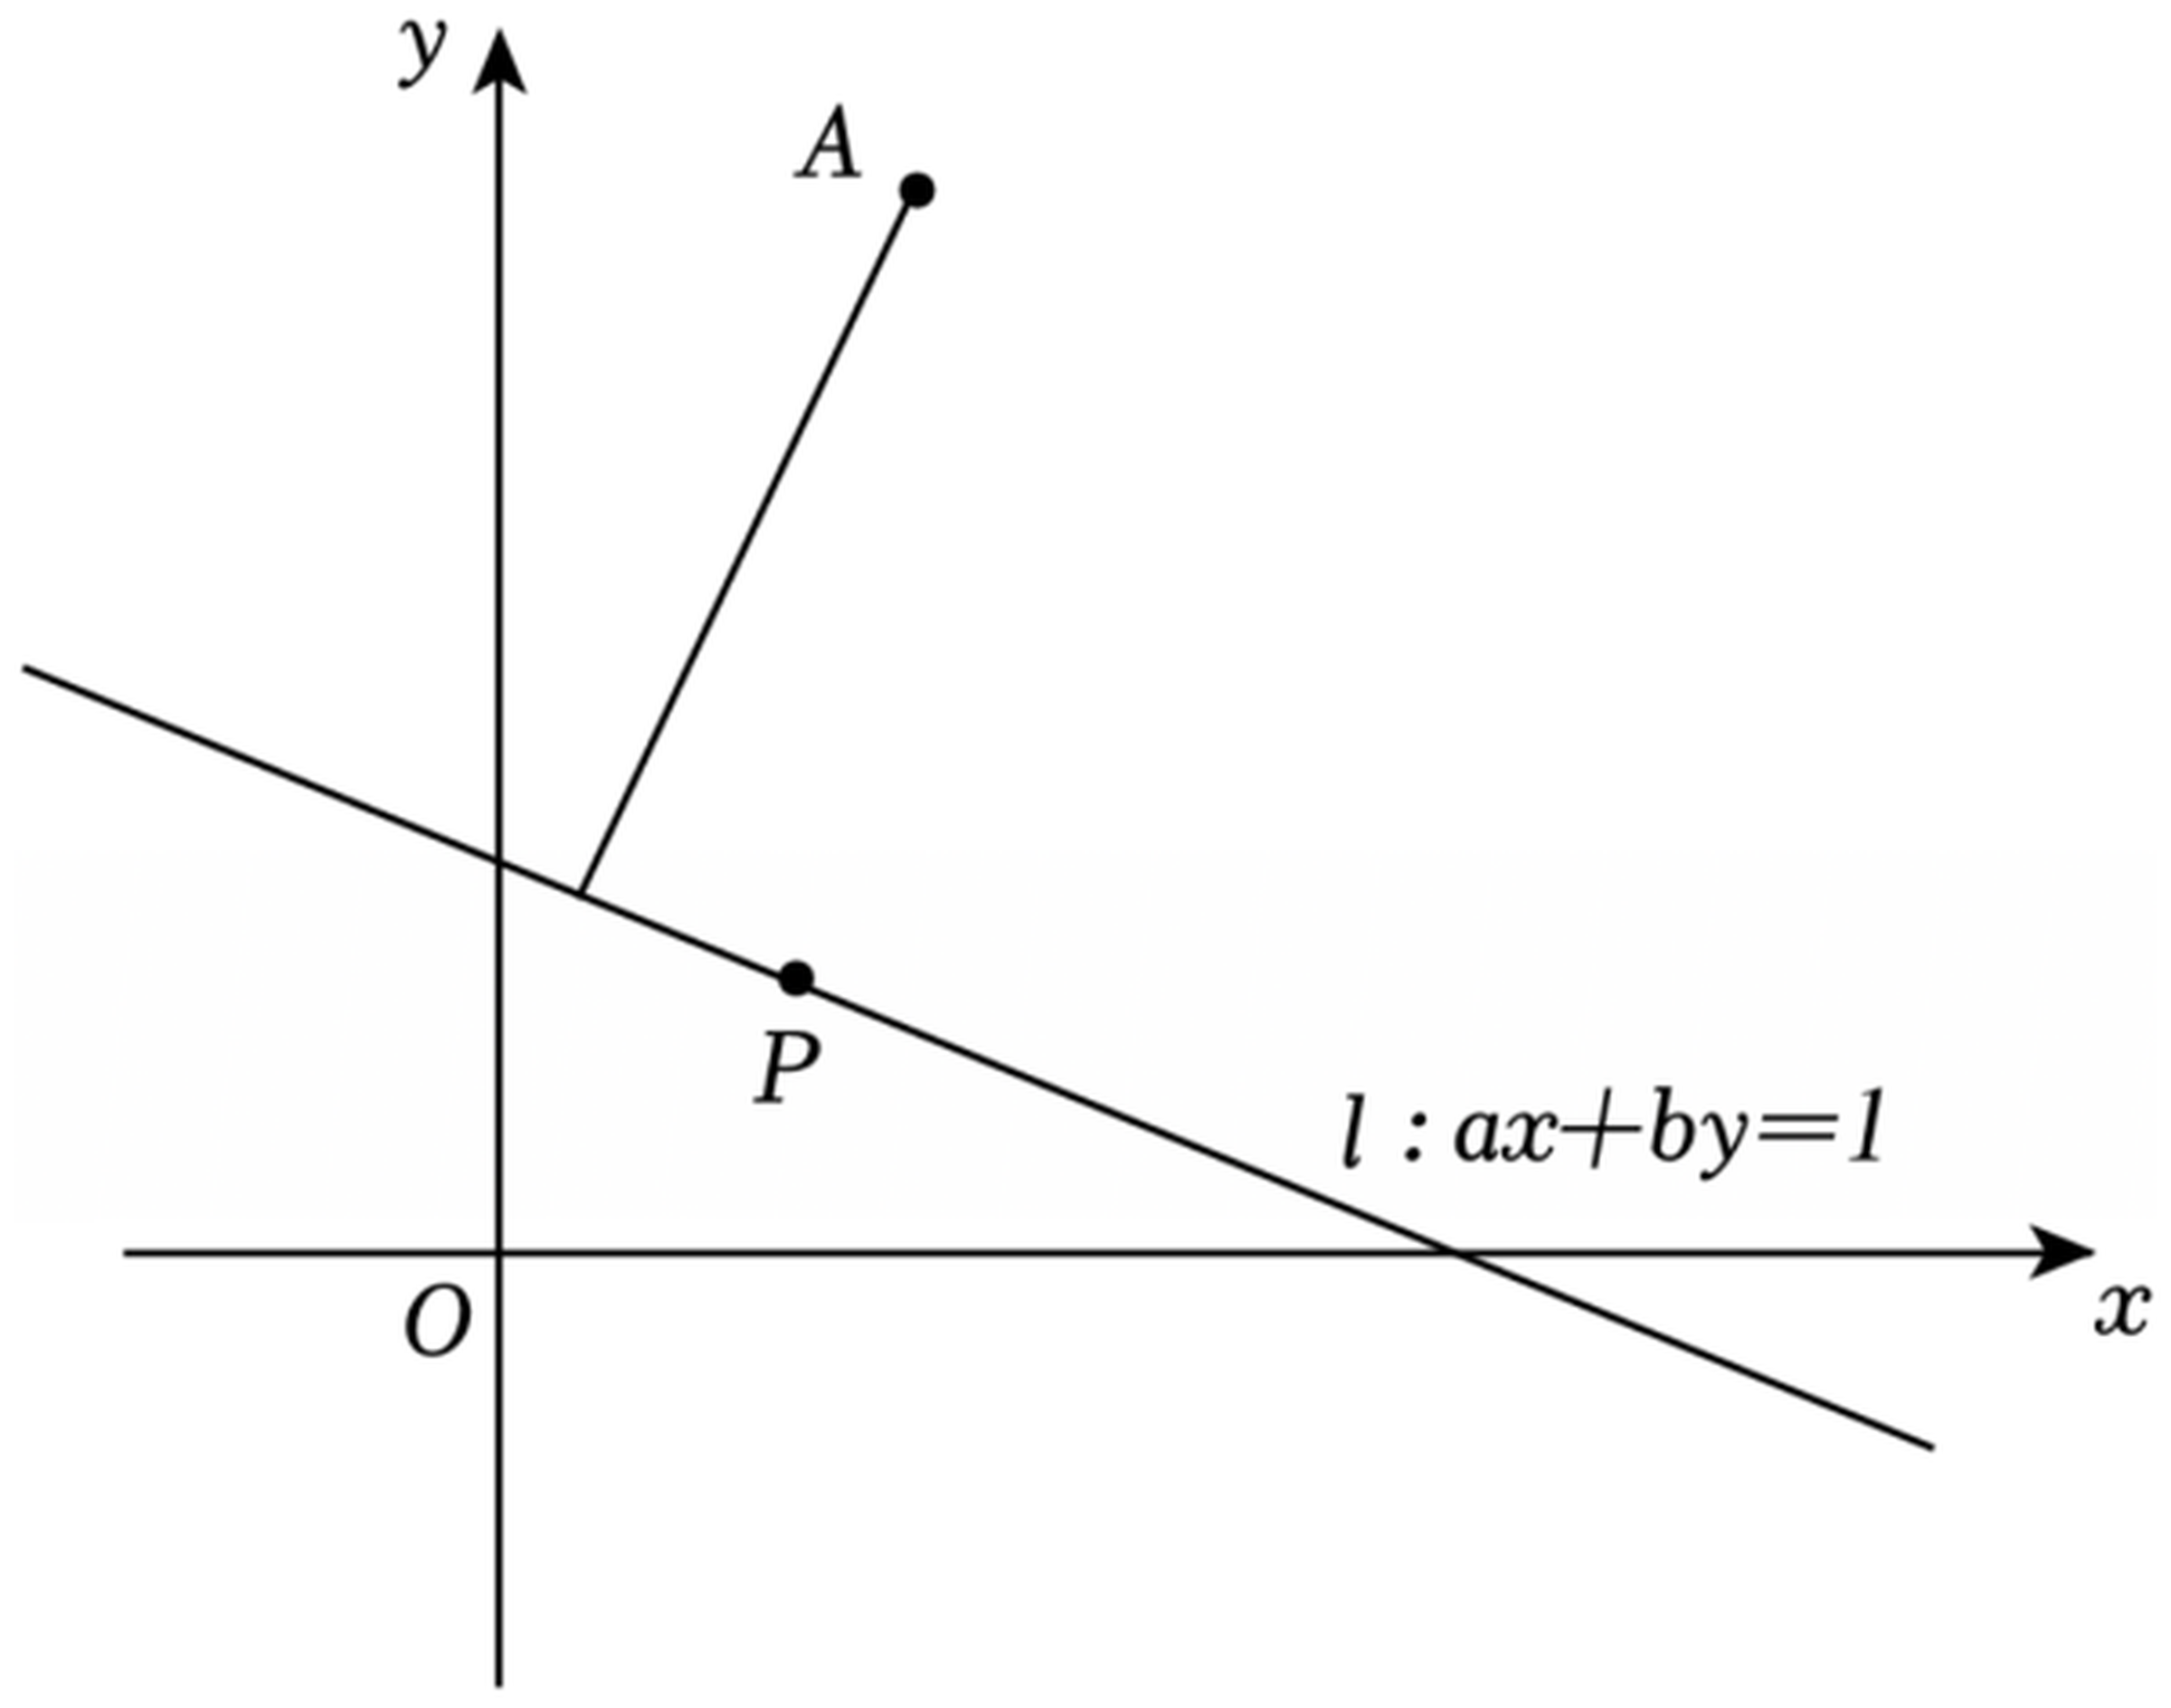
\includegraphics[width=0.56\textwidth]{figures/line_ax_plus_by_1.png}
\end{center}

\step{因为 $a+b=2$，所以直线 $l$ 恒过定点 $P\left(\dfrac12,\dfrac12\right)$，}
\step{再令 $A(1,2)$，则
$d_{A-l}=\dfrac{|a+2b-1|}{\sqrt{a^2+b^2}}\leqslant|AP|=\dfrac{\sqrt{10}}2$，}
\step{当且仅当 $l\perp AP$ 时等号成立，}
\step{又 $\dfrac{a+2b-1}{\sqrt{a^2+b^2}}\leqslant\dfrac{|a+2b-1|}{\sqrt{a^2+b^2}}$，
而当 $l\perp AP$，$a+2b-1>0$，等号也成立，}
\step{故 $\left(\dfrac{a+2b-1}{\sqrt{a^2+b^2}}\right)_{\max}=\dfrac{\sqrt{10}}2$.}
\solend

\fi

\ansspace[6]

\item （1）设 $a$、$b$、$c$ 都是正数，试证明不等式：
$\dfrac{b+c}a+\dfrac{c+a}b+\dfrac{a+b}c\geqslant6$；

（2）对一切正整数 $n$，不等式 $\dfrac{2x-1}x>\dfrac n{n+1}$ 恒成立，
则实数 $x$ 的取值范围构成的集合.

\ifanswer
\solbegin
\stepm{(1)}{因为 $a>0$，$b>0$，$c>0$，}
\step{所以 $\dfrac ba+\dfrac ab\geqslant2$，$\dfrac ca+\dfrac ac\geqslant2$，
$\dfrac cb+\dfrac bc\geqslant2$，}
\step{所以 $\left(\dfrac ba+\dfrac ab\right)+\left(\dfrac ca+\dfrac ac\right)
+\left(\dfrac cb+\dfrac bc\right)\geqslant6$，
即 $\dfrac{b+c}a+\dfrac{c+a}b+\dfrac{a+b}c\geqslant6$.}
% 注：下一行题干原卷作「……则实数 $x$ 的取值范围构成的集合.」，缺一个「求」字，
%     照抄未改，见文件头「原卷存疑」⑤。
\stepm{(2)}{考查 $y=\dfrac n{n+1}=1-\dfrac1{n+1}$，一切正整数 $n$ 函数为严格增函数，
所以 $y\geqslant\dfrac12$，}
\step{对一切正整数 $n$，不等式 $\dfrac{2x-1}x>\dfrac n{n+1}$ 恒成立，
所以 $\dfrac{2x-1}x\geqslant1$，}
\step{所以 $\dfrac{x-1}x\geqslant0$，所以 $x<0$ 或 $x\geqslant1$，}
\step{所以实数 $x$ 的取值范围是 $(-\infty,0)\cup[1,+\infty)$.}
\solend

\fi

\ansspace[6]

\end{enumerate}

\end{document}
"
% 紧凑版：xelatex "\def\iscompact{1}% 高一34_交附闵行_查漏补缺卷.tex
%   —— 高一上数学「2026-2027 年交附闵行高一上查漏补缺卷」（试卷版/答案版）
% 试卷版：xelatex 高一34_交附闵行_查漏补缺卷.tex
% 答案版：xelatex "\def\isanswer{1}\input{高一34_交附闵行_查漏补缺卷.tex}"
% 紧凑版：xelatex "\def\iscompact{1}\input{高一34_交附闵行_查漏补缺卷.tex}"
%
% 原始材料是微信公众号图文（公众号「魔都数学加油站」连载「27学年高一 34」，2026-09-25 发布，
% 原文标题「27学年高一34——2026-2027年上海市交附闵行高一上查漏补缺卷」），
% 正文为 7 张 PNG 页（均 2560×3620），取 mmbiz.qpic.cn/<hash>/0 的原图档。
% 原文本身就是一份**讲评版**，但**全卷没有任何一处印「【答案】」**——每题下方直接印【解析】，
% 答案写在解析的末句。试题文字与解析均照原卷录入，未改内容。
% 卷面的粉色斜水印属水印，未录入。
%
% 卷首标题：原卷印作「2026-2027 年交附闵行高一上查漏补缺卷」（公众号标题里的「上海市」
% 三字卷面标题行没有，本稿照卷面），年份区间按全稿惯例排 en dash，前缀照原卷保留「年」。
%
% 与原卷的排版差异（均已在 README「说明」中交代）：
%   ① 原文自**第 3 题**起（第 1、2 题未在该文中发布），故本稿题号亦自 3 起；
%   ② 原卷只有「一、填空题」「二、解答题」两个节标题（本卷无选择题），本稿照原卷分节，
%      只把标题改排成全稿统一的「大节标题」样式；
%   ③ 原卷通篇只印【解析】（无【答案】行），本稿统一改为试卷版隐去、答案版以 \ifanswer{}
%      块给出，两版彻底分离；
%   ④ 数集记号原卷两套并用：第 4 题与第 11(2) 题作斜体的 $R$，第 7 题两处作粗体的
%      $\mathbf{R}^+$，本稿按全稿惯例统一写作 $\R$；
%   ⑤ 原卷填空的横线约两个字宽，本稿按全稿惯例统一排 \blankline[4.4em]（第 9 题的第一个空
%      原卷**没有**下划线、只留了一个空格，本稿仍补出横线，见文件头「原卷存疑」①）；
%   ⑥ 原卷未印副标题，本稿按全稿惯例补出副标题「集合与常用逻辑用语」（本卷实为基本不等式
%      专题，与 高一27／高一28 同样只标主章节，见文末「高一34 专记」）；
%   ⑦ 第 13 题的配图只出现在【解析】里（题干并未写「如图」），故放进 \ifanswer 块，
%      试卷版不排；图取原卷截图、4× LANCZOS 放大（figures/line_ax_plus_by_1.png）。
%
% 原卷存疑五处（均照抄原卷、未改，见源码中该处上方注释）：
%   ① 第 9 题「则 $ab$ 的最大值为 ，」——第一个空后面只有空格、没有下划线，第二个空才有；
%   ② 第 11(2) 题题干括号内写「$a$、$b\in R$」，但函数式 $f(x)=ax^2+(3a-4)x-12$ 里并没有 $b$；
%   ③ 第 10 题只限定 $a$ 是正实数，未提 $b$ 的取值范围；
%   ④ 第 13 题题干作「求 …… 的最大值为____.」（「求」与「为」混用），且**题干未写「如图」**，
%      是【解析】里才写「如图」；
%   ⑤ 第 14(2) 题题干作「……则实数 $x$ 的取值范围构成的集合.」——缺一个「求」字。
% 另有两处标点照录：第 9 题【解析】首句末是句号、第 11(1)① 解析末句是分号。

\documentclass[a4paper,11pt]{article}
\usepackage{common}

\begin{document}

\examtitlest[3]{2026--2027 年交附闵行高一上查漏补缺卷}{集合与常用逻辑用语}

\bigsec{一、填空题}

\begin{enumerate}
\setcounter{enumi}{2}

\item 已知正实数 $m$、$n$ 满足 $\dfrac1{m+2n}+\dfrac1{2m+n}=1$，则 $m+n$ 的最小值为
\blankline[4.4em].

\ifanswer
\solbegin
\step{因为 $m$、$n\in(0,+\infty)$，$\dfrac1{m+2n}+\dfrac1{2m+n}=1$，}
\step{所以 $m+n=\dfrac13[(m+2n)+(2m+n)]\left(\dfrac1{m+2n}+\dfrac1{2m+n}\right)$}
\step{$=\dfrac13\left[2+\dfrac{2m+n}{m+2n}+\dfrac{m+2n}{2m+n}\right]
\geqslant\dfrac13\left[2+2\sqrt{\dfrac{2m+n}{m+2n}\cdot\dfrac{m+2n}{2m+n}}\right]
=\dfrac43$，}
\step{当且仅当 $\dfrac{2m+n}{m+2n}=\dfrac{m+2n}{2m+n}$，即 $m=n=\dfrac23$ 时取等号，}
\step{所以 $m+n$ 的最小值为 $\dfrac43$.}
\solend

\fi

\item 若 $a$、$b\in\R$，且 $a^2+2ab-3b^2=1$，则 $a^2+b^2$ 的最小值为 \blankline[4.4em].

\ifanswer
\solbegin
\step{由 $a^2+2ab-3b^2=1$ 得 $(a+3b)(a-b)=1$，}
\step{令 $x=a+3b$，$y=a-b$，则 $xy=1$ 且 $a=\dfrac{x+3y}4$，$b=\dfrac{x-y}4$，}
\step{所以 $a^2+b^2=\left(\dfrac{x+3y}4\right)^2+\left(\dfrac{x-y}4\right)^2
=\dfrac{x^2+5y^2+2}8\geqslant\dfrac{2\sqrt{5x^2y^2}+2}8=\dfrac{\sqrt5+1}4$，}
\step{当且仅当 $x^2=\sqrt5$，$y^2=\dfrac{\sqrt5}5$ 时取等号，
故 $a^2+b^2$ 的最小值为 $\dfrac{\sqrt5+1}4$.}
\solend

\fi

\item 已知实数 $x$、$y$ 满足 $3x^2+3y^2-2xy=4$，则 $x+y$ 的最大值为 \blankline[4.4em].

\ifanswer
\solbegin
\step{由 $3x^2+3y^2-2xy=4$，则 $3[(x+y)^2-2xy]-2xy=4$，}
\step{设 $s=x+y$，则 $3s^2-8xy=4$，即 $xy=\dfrac{3s^2-4}8$，}
\step{对任意实数 $x$、$y$，有 $xy\leqslant\left(\dfrac{x+y}2\right)^2=\dfrac{s^2}4$，
即 $\dfrac{3s^2-4}8\leqslant\dfrac{s^2}4$，}
\step{得 $s^2\leqslant4$，即 $-2\leqslant s\leqslant2$，}
\step{当 $x=y=1$ 时，满足原等式，且 $x+y=2$ 成立，因此 $x+y$ 的最大值为 $2$.}
\solend

\fi

\item 若 $a$、$b$、$c$ 都是正实数，则 $\dfrac{a^2+2b^2+4c^2}{ab+2bc}$ 的最小值为
\blankline[4.4em].

\ifanswer
\solbegin
\step{因为 $a^2+2b^2+4c^2=a^2+b^2+b^2+4c^2=(a^2+b^2)+(b^2+4c^2)\geqslant2ab+4bc$，}
\step{所以 $\dfrac{a^2+2b^2+4c^2}{ab+2bc}\geqslant\dfrac{2ab+4bc}{ab+2bc}=2$，
当且仅当 $a=b=2c$ 时取等号，}
\step{即 $\dfrac{a^2+2b^2+4c^2}{ab+2bc}$ 的最小值是 $2$.}
\solend

\fi

\item 已知 $a$、$b\in\R^+$，且 $ab=2$，则 $\dfrac b{2+a^2}+\dfrac a{2+b^2}$ 的最小值是
\blankline[4.4em].

\ifanswer
\solbegin
\step{$\dfrac b{2+a^2}+\dfrac a{2+b^2}=\dfrac b{ab+a^2}+\dfrac a{ab+b^2}
=\dfrac b{a(a+b)}+\dfrac a{b(a+b)}$}
\step{$=\dfrac{(a+b)^2-4}{2(a+b)}=\dfrac{a+b}2-\dfrac2{a+b}$，}
\step{令 $t=a+b$，则原式可设为 $y=\dfrac t2-\dfrac2t$ 的函数，}
\step{当 $t>0$ 时，此函数为严格增函数，}
\step{因为 $a$、$b\in\R^+$ 且 $ab=2$，$t=a+b\geqslant2\sqrt{ab}=2\sqrt2$，}
\step{当且仅当 $a=b=\sqrt2$ 时，$t$ 的最小值为 $2\sqrt2$，}
\step{$y=\dfrac t2-\dfrac2t$ 在 $t\in[2\sqrt2,+\infty)$ 上严格增，}
\step{所以原式的最小值为 $\dfrac{2\sqrt2}2-\dfrac2{2\sqrt2}=\dfrac{\sqrt2}2$，
则 $\dfrac b{2+a^2}+\dfrac a{2+b^2}$ 的最小值是 $\dfrac{\sqrt2}2$.}
\solend

\fi

\item 设 $x$、$y$、$z$ 为正实数，满足 $x-2y+3z=0$，则 $\dfrac{y^2}{xz}$ 的最小值是
\blankline[4.4em].

\ifanswer
\solbegin
\step{因为 $x-2y+3z=0$，所以 $y=\dfrac{x+3z}2$，}
\step{所以 $\dfrac{y^2}{xz}=\dfrac{x^2+9z^2+6xz}{4xz}\geqslant\dfrac{6xz+6xz}{4xz}=3$，
当且仅当 $x=3z$ 时取等号，}
\step{故 $\dfrac{y^2}{xz}$ 的最小值是 $3$.}
\solend

\fi

% 注：下一题的第一个空原卷只留了一个空格、**没有**下划线（第二个空才有），本稿仍按全稿
%     惯例补出横线；另其【解析】首句末原卷作句号，照录。见文件头「原卷存疑」①。
\item 设 $a$、$b$ 为正实数，且 $a+b=3$，则 $ab$ 的最大值为 \blankline[4.4em]，
$\dfrac{a^2}{a+2}+\dfrac{b^2}{b+1}$ 的最小值为 \blankline[4.4em].

\ifanswer
\solbegin
\step{因为 $a>0$，$b>0$，所以 $a+b=3\geqslant2\sqrt{ab}$，}
\step{故 $ab$ 的最大值为 $\dfrac94$，当且仅当 $a=b=\dfrac32$ 时取等号.}
\step{令 $a+2=m$，$b+1=n$，则 $m+n=a+b+3=6$，}
\step{解得 $a=m-2$，$b=n-1$，}
\step{所以 $\dfrac{a^2}{a+2}+\dfrac{b^2}{b+1}=\dfrac{(m-2)^2}m+\dfrac{(n-1)^2}n
=m+\dfrac4m+n+\dfrac1n-6=\dfrac4m+\dfrac1n$}
\step{$=\dfrac16(m+n)\left(\dfrac4m+\dfrac1n\right)
=\dfrac16\left(\dfrac{4n}m+\dfrac mn+5\right)\geqslant\dfrac16(4+5)=\dfrac32$，}
\step{当且仅当 $\dfrac{4n}m=\dfrac mn$ 时，即 $m=2n$ 时
$\dfrac{a^2}{a+2}+\dfrac{b^2}{b+1}$ 取得最小值，}
\step{因此 $\dfrac{a^2}{a+2}+\dfrac{b^2}{b+1}$ 的最小值为 $\dfrac32$.}
\solend

\fi

\item 若 $a$ 是正实数，$2a^2+3b^2=10$，则 $a\sqrt{2+b^2}$ 的最大值是 \blankline[4.4em].

\ifanswer
\solbegin
\step{$a$ 是正实数，$2a^2+3b^2=10$，变形为 $2a^2+3(b^2+2)=16$，}
\step{所以 $16\geqslant2\sqrt{2a^2\times3(b^2+2)}=2\sqrt6\cdot a\sqrt{b^2+2}$，
得 $a\sqrt{2+b^2}\leqslant\dfrac{4\sqrt6}3$，}
\step{当且仅当 $2a^2=3(b^2+2)=8$，即 $a=2$，$b^2=\dfrac23$ 时取等号，}
\step{所以 $a\sqrt{2+b^2}$ 的最大值为 $\dfrac{4\sqrt6}3$.}
\solend

\fi

\end{enumerate}

\bigsec{二、解答题}

\begin{enumerate}
\setcounter{enumi}{10}

\item （1）已知 $x>0$，$y>0$，$2xy=x+4y$. ①求 $xy$ 的最小值；②求 $x+y$ 的最小值.

（2）已知函数 $f(x)=ax^2+(3a-4)x-12$（$a$、$b\in\R$），求不等式 $f(x)\geqslant0$ 的解集.

\ifanswer
\solbegin
\stepm{(1)}{①因为 $x>0$，$y>0$，由基本不等式得
$2xy=x+4y\geqslant2\sqrt{4xy}=4\sqrt{xy}$，}
\step{解得 $xy\geqslant4$，当且仅当 $x=4y=4$ 时取等号，故 $xy$ 的最小值为 $4$；}
\step{②因为 $x>0$，$y>0$，由已知条件得 $\dfrac{4y+x}{xy}=\dfrac4x+\dfrac1y=2$，}
\step{所以 $x+y=\dfrac12(x+y)\left(\dfrac4x+\dfrac1y\right)
=\dfrac12\left(5+\dfrac{4y}x+\dfrac xy\right)
\geqslant\dfrac12\left(5+2\sqrt{\dfrac{4y}x\cdot\dfrac xy}\right)=\dfrac92$，}
\step{当且仅当 $x=2y=3$ 时，等号成立，故 $x+y$ 的最小值为 $\dfrac92$；}
% 注：下一行题干括号内原卷写「$a$、$b\in R$」，但函数式里并没有 $b$，照抄未改，
%     见文件头「原卷存疑」②。
\stepm{(2)}{当 $a=0$ 时，则 $x+3\leqslant0$，解得 $x\leqslant-3$；}
\step{当 $a\neq0$ 时，$f(x)=ax^2+(3a-4)x-12=(x+3)(ax-4)
=a(x+3)\left(x-\dfrac4a\right)$，}
\step{当 $a>0$ 时，则 $(x+3)\left(x-\dfrac4a\right)\geqslant0$，
解得 $x\leqslant-3$ 或 $x\geqslant\dfrac4a$；}
\step{当 $a<0$ 时，则 $(x+3)\left(x-\dfrac4a\right)\leqslant0$，}
\step{当 $\dfrac4a>-3$ 时，即 $a<-\dfrac43$，解 $(x+3)\left(x-\dfrac4a\right)\leqslant0$，
得 $-3\leqslant x\leqslant\dfrac4a$；}
\step{当 $\dfrac4a=-3$ 时，即 $a=-\dfrac43$，解 $(x+3)\left(x-\dfrac4a\right)\leqslant0$，
得 $x=-3$；}
\step{当 $\dfrac4a<-3$ 时，即 $-\dfrac43<a<0$，解 $(x+3)\left(x-\dfrac4a\right)\leqslant0$，
得 $\dfrac4a\leqslant x\leqslant-3$；}
\step{综上所述，当 $a<-\dfrac43$ 时，不等式 $f(x)\geqslant0$ 的解集为
$\left[-3,\dfrac4a\right]$；}
\step{当 $a=-\dfrac43$ 时，不等式 $f(x)\geqslant0$ 的解集为 $\{-3\}$；}
\step{当 $-\dfrac43<a<0$ 时，不等式 $f(x)\geqslant0$ 的解集为
$\left[\dfrac4a,-3\right]$；}
\step{当 $a=0$ 时，不等式 $f(x)\geqslant0$ 的解集为 $(-\infty,-3]$；}
\step{当 $a>0$ 时，不等式 $f(x)\geqslant0$ 的解集为
$(-\infty,-3]\cup\left[\dfrac4a,+\infty\right)$.}
\solend

\fi

\ansspace[8]

\item 已知 $x$、$y$ 都是正数，且 $\dfrac2x+\dfrac1y=1$.

\begin{enumerate}[label=(\arabic*)]
\item 求 $2x+y$ 的最小值及此时 $x$、$y$ 的取值；
\item 不等式 $(2x+y)^2\geqslant m(x+2y)$ 恒成立，求实数 $m$ 的取值范围.
\end{enumerate}

\ifanswer
\solbegin
\stepm{(1)}{$2x+y=(2x+y)\left(\dfrac2x+\dfrac1y\right)
=4+\dfrac{2x}y+\dfrac{2y}x+1\geqslant5+2\sqrt{\dfrac{2x}y\cdot\dfrac{2y}x}=9$，}
\step{当且仅当 $x=y$ 且 $\dfrac2x+\dfrac1y=1$，即 $x=y=3$ 时取等号，}
\step{此时 $2x+y$ 的最小值为 $9$.}
\stepm{(2)}{由 $\dfrac2x+\dfrac1y=1$，得 $x+2y=xy>0$，}
\step{故 $(2x+y)^2\geqslant m(x+2y)\Leftrightarrow m\leqslant\dfrac{(2x+y)^2}{x+2y}
\Leftrightarrow m\leqslant\dfrac{(2x+y)^2}{xy}$，}
\step{又 $\dfrac{(2x+y)^2}{xy}=\dfrac{4x^2+y^2+4xy}{xy}
=\dfrac{4x}y+\dfrac yx+4\geqslant2\sqrt{\dfrac{4x}y\cdot\dfrac yx}+4=8$，}
\step{当且仅当 $\begin{cases}\dfrac{4x}y=\dfrac yx\\[2pt]
\dfrac2x+\dfrac1y=1\end{cases}$ 时取等号，$\dfrac{(2x+y)^2}{xy}$ 取得最小值 $8$，}
\step{故 $m$ 的取值范围为 $\{m\mid m\leqslant8\}$.}
\solend

\fi

\ansspace[6]

% 注：本小题题干作「求 …… 的最大值为____.」（「求」与「为」混用），且**题干未写「如图」**
%     ——是【解析】里才写「如图」，照抄未改，见文件头「原卷存疑」④。
\item 已知实数 $a$、$b$ 满足 $a+b=2$，求 $\dfrac{a+2b-1}{\sqrt{a^2+b^2}}$ 的最大值为
\blankline[4.4em].

\ifanswer
\solbegin
\step{如图，考虑直线 $l:ax+by=1$，}

\begin{center}
% 图取原卷截图、4× LANCZOS 放大。图只在【解析】里出现（题干并未写「如图」），
% 故放进 \ifanswer 块，试卷版不排，见文件头⑦。
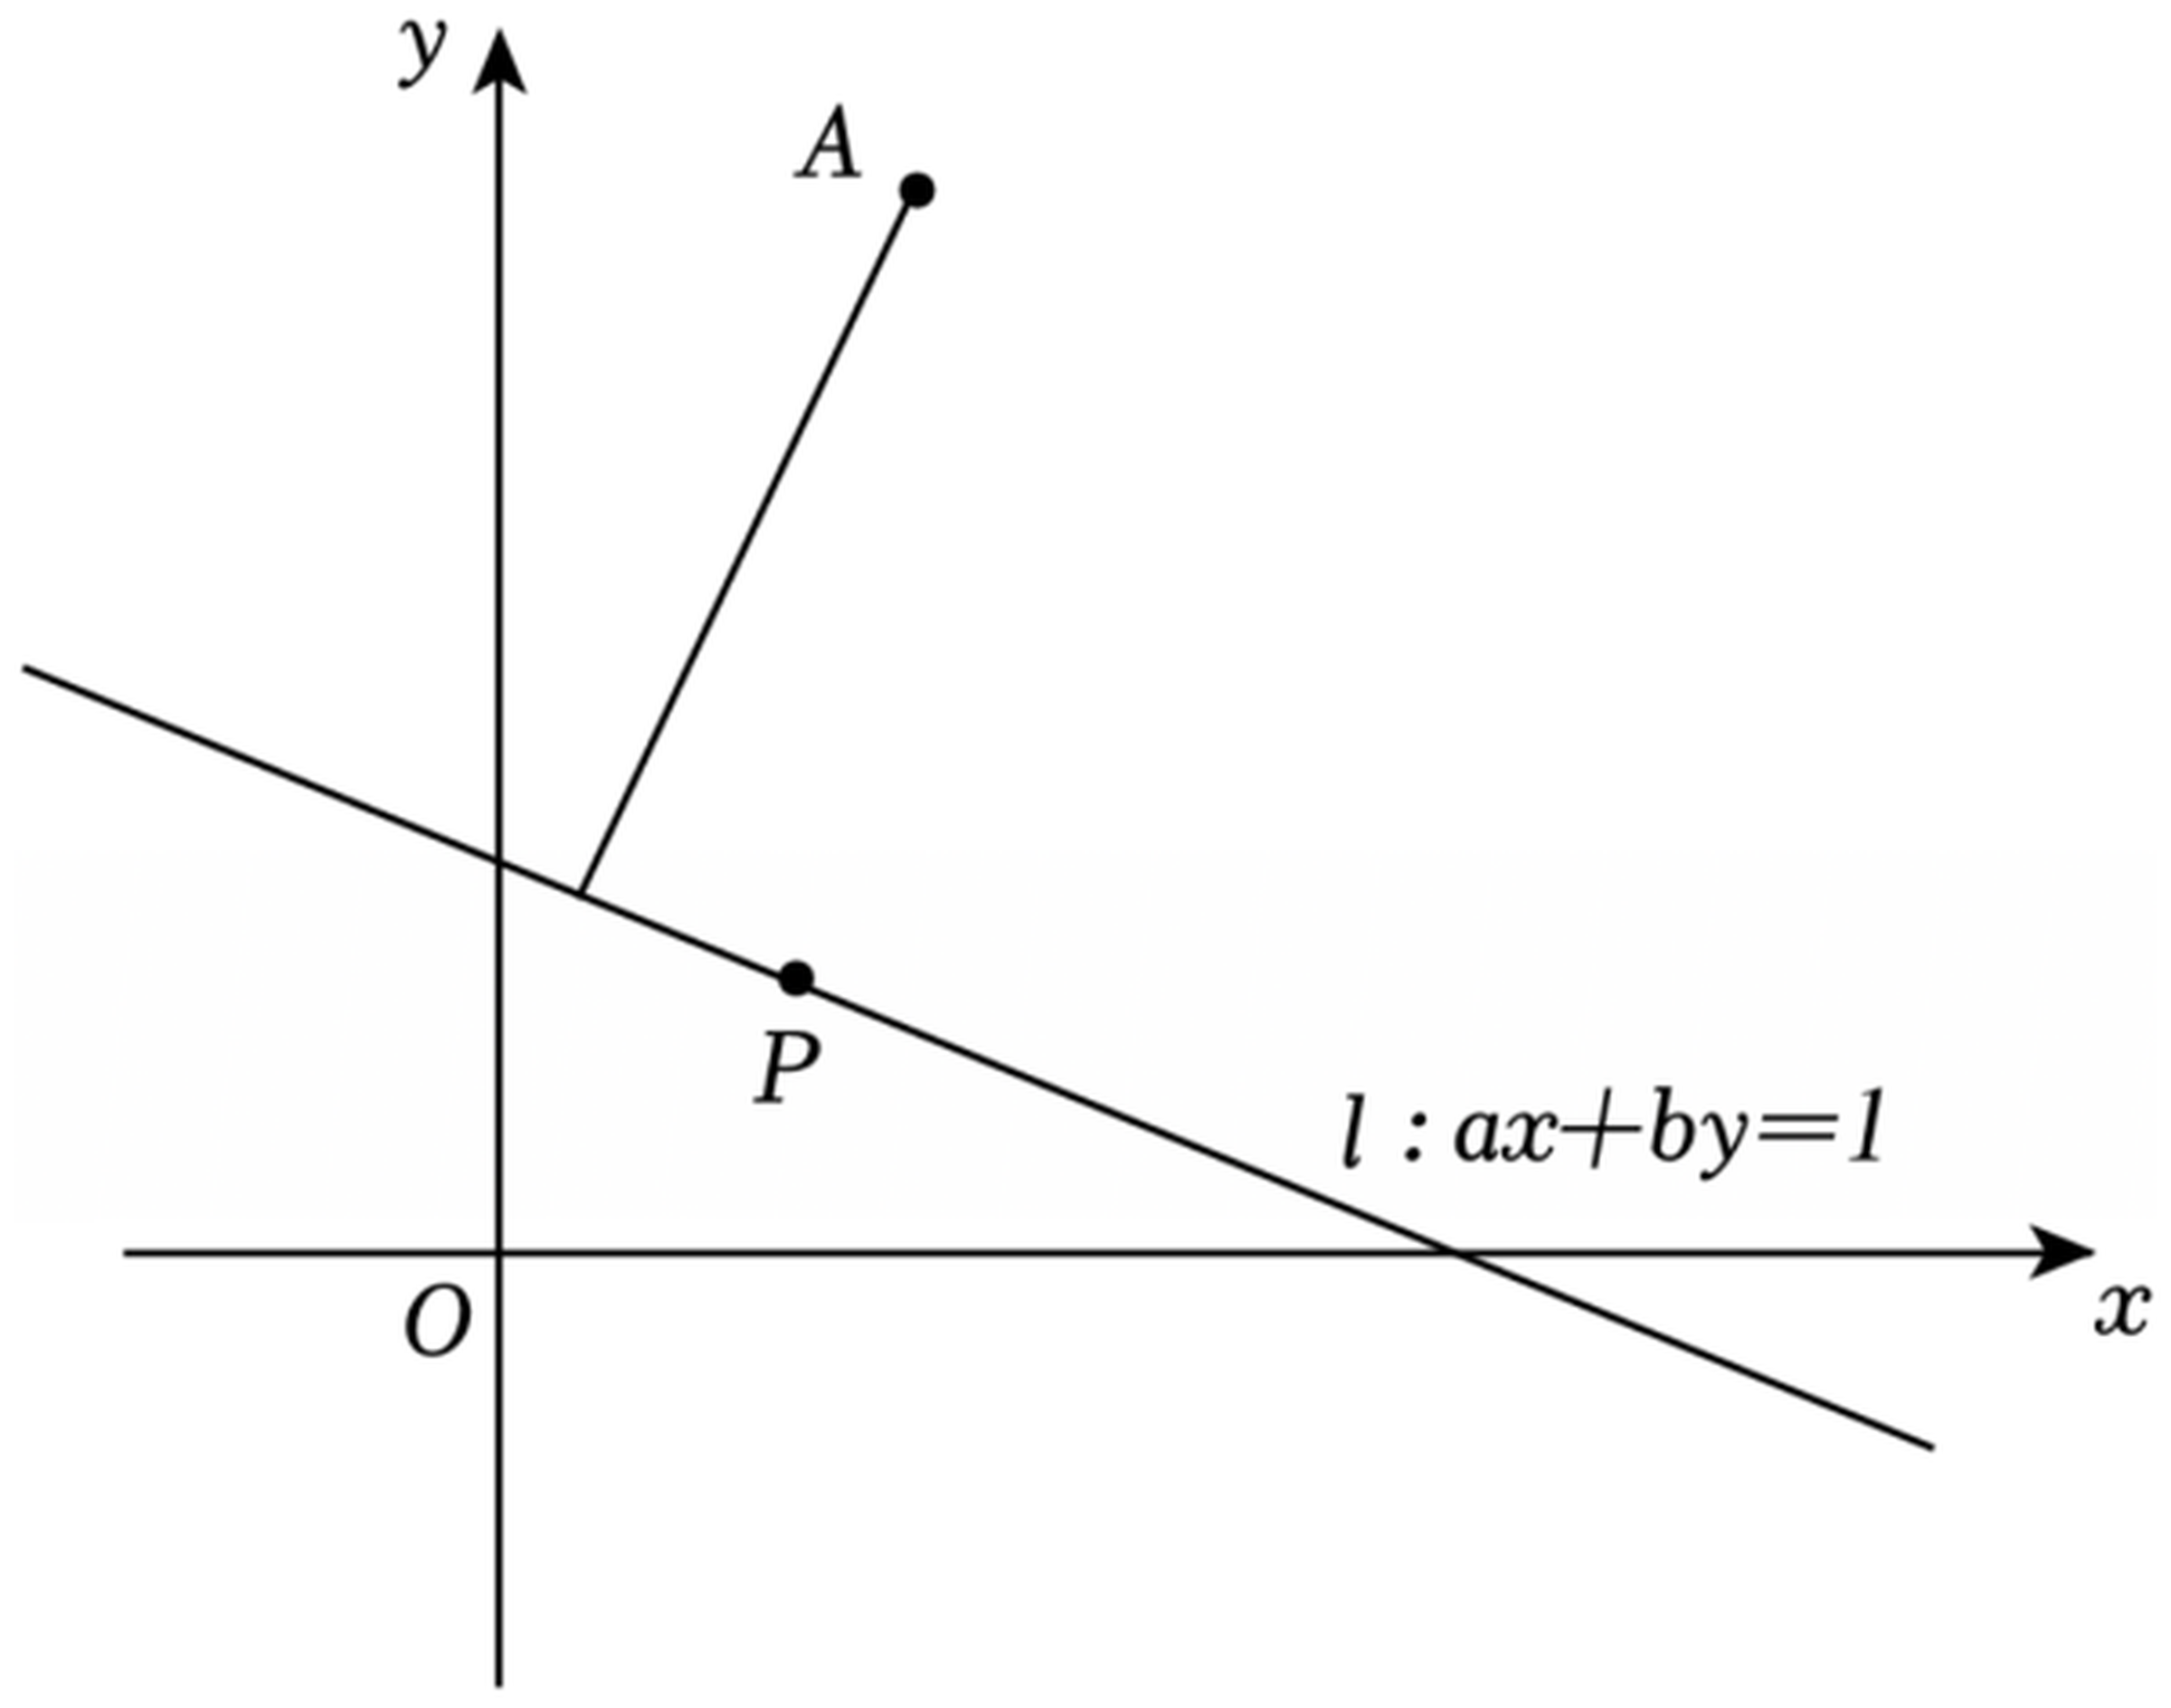
\includegraphics[width=0.56\textwidth]{figures/line_ax_plus_by_1.png}
\end{center}

\step{因为 $a+b=2$，所以直线 $l$ 恒过定点 $P\left(\dfrac12,\dfrac12\right)$，}
\step{再令 $A(1,2)$，则
$d_{A-l}=\dfrac{|a+2b-1|}{\sqrt{a^2+b^2}}\leqslant|AP|=\dfrac{\sqrt{10}}2$，}
\step{当且仅当 $l\perp AP$ 时等号成立，}
\step{又 $\dfrac{a+2b-1}{\sqrt{a^2+b^2}}\leqslant\dfrac{|a+2b-1|}{\sqrt{a^2+b^2}}$，
而当 $l\perp AP$，$a+2b-1>0$，等号也成立，}
\step{故 $\left(\dfrac{a+2b-1}{\sqrt{a^2+b^2}}\right)_{\max}=\dfrac{\sqrt{10}}2$.}
\solend

\fi

\ansspace[6]

\item （1）设 $a$、$b$、$c$ 都是正数，试证明不等式：
$\dfrac{b+c}a+\dfrac{c+a}b+\dfrac{a+b}c\geqslant6$；

（2）对一切正整数 $n$，不等式 $\dfrac{2x-1}x>\dfrac n{n+1}$ 恒成立，
则实数 $x$ 的取值范围构成的集合.

\ifanswer
\solbegin
\stepm{(1)}{因为 $a>0$，$b>0$，$c>0$，}
\step{所以 $\dfrac ba+\dfrac ab\geqslant2$，$\dfrac ca+\dfrac ac\geqslant2$，
$\dfrac cb+\dfrac bc\geqslant2$，}
\step{所以 $\left(\dfrac ba+\dfrac ab\right)+\left(\dfrac ca+\dfrac ac\right)
+\left(\dfrac cb+\dfrac bc\right)\geqslant6$，
即 $\dfrac{b+c}a+\dfrac{c+a}b+\dfrac{a+b}c\geqslant6$.}
% 注：下一行题干原卷作「……则实数 $x$ 的取值范围构成的集合.」，缺一个「求」字，
%     照抄未改，见文件头「原卷存疑」⑤。
\stepm{(2)}{考查 $y=\dfrac n{n+1}=1-\dfrac1{n+1}$，一切正整数 $n$ 函数为严格增函数，
所以 $y\geqslant\dfrac12$，}
\step{对一切正整数 $n$，不等式 $\dfrac{2x-1}x>\dfrac n{n+1}$ 恒成立，
所以 $\dfrac{2x-1}x\geqslant1$，}
\step{所以 $\dfrac{x-1}x\geqslant0$，所以 $x<0$ 或 $x\geqslant1$，}
\step{所以实数 $x$ 的取值范围是 $(-\infty,0)\cup[1,+\infty)$.}
\solend

\fi

\ansspace[6]

\end{enumerate}

\end{document}
"
%
% 原始材料是微信公众号图文（公众号「魔都数学加油站」连载「27学年高一 34」，2026-09-25 发布，
% 原文标题「27学年高一34——2026-2027年上海市交附闵行高一上查漏补缺卷」），
% 正文为 7 张 PNG 页（均 2560×3620），取 mmbiz.qpic.cn/<hash>/0 的原图档。
% 原文本身就是一份**讲评版**，但**全卷没有任何一处印「【答案】」**——每题下方直接印【解析】，
% 答案写在解析的末句。试题文字与解析均照原卷录入，未改内容。
% 卷面的粉色斜水印属水印，未录入。
%
% 卷首标题：原卷印作「2026-2027 年交附闵行高一上查漏补缺卷」（公众号标题里的「上海市」
% 三字卷面标题行没有，本稿照卷面），年份区间按全稿惯例排 en dash，前缀照原卷保留「年」。
%
% 与原卷的排版差异（均已在 README「说明」中交代）：
%   ① 原文自**第 3 题**起（第 1、2 题未在该文中发布），故本稿题号亦自 3 起；
%   ② 原卷只有「一、填空题」「二、解答题」两个节标题（本卷无选择题），本稿照原卷分节，
%      只把标题改排成全稿统一的「大节标题」样式；
%   ③ 原卷通篇只印【解析】（无【答案】行），本稿统一改为试卷版隐去、答案版以 \ifanswer{}
%      块给出，两版彻底分离；
%   ④ 数集记号原卷两套并用：第 4 题与第 11(2) 题作斜体的 $R$，第 7 题两处作粗体的
%      $\mathbf{R}^+$，本稿按全稿惯例统一写作 $\R$；
%   ⑤ 原卷填空的横线约两个字宽，本稿按全稿惯例统一排 \blankline[4.4em]（第 9 题的第一个空
%      原卷**没有**下划线、只留了一个空格，本稿仍补出横线，见文件头「原卷存疑」①）；
%   ⑥ 原卷未印副标题，本稿按全稿惯例补出副标题「集合与常用逻辑用语」（本卷实为基本不等式
%      专题，与 高一27／高一28 同样只标主章节，见文末「高一34 专记」）；
%   ⑦ 第 13 题的配图只出现在【解析】里（题干并未写「如图」），故放进 \ifanswer 块，
%      试卷版不排；图取原卷截图、4× LANCZOS 放大（figures/line_ax_plus_by_1.png）。
%
% 原卷存疑五处（均照抄原卷、未改，见源码中该处上方注释）：
%   ① 第 9 题「则 $ab$ 的最大值为 ，」——第一个空后面只有空格、没有下划线，第二个空才有；
%   ② 第 11(2) 题题干括号内写「$a$、$b\in R$」，但函数式 $f(x)=ax^2+(3a-4)x-12$ 里并没有 $b$；
%   ③ 第 10 题只限定 $a$ 是正实数，未提 $b$ 的取值范围；
%   ④ 第 13 题题干作「求 …… 的最大值为____.」（「求」与「为」混用），且**题干未写「如图」**，
%      是【解析】里才写「如图」；
%   ⑤ 第 14(2) 题题干作「……则实数 $x$ 的取值范围构成的集合.」——缺一个「求」字。
% 另有两处标点照录：第 9 题【解析】首句末是句号、第 11(1)① 解析末句是分号。

\documentclass[a4paper,11pt]{article}
\usepackage{common}

\begin{document}

\examtitlest[3]{2026--2027 年交附闵行高一上查漏补缺卷}{集合与常用逻辑用语}

\bigsec{一、填空题}

\begin{enumerate}
\setcounter{enumi}{2}

\item 已知正实数 $m$、$n$ 满足 $\dfrac1{m+2n}+\dfrac1{2m+n}=1$，则 $m+n$ 的最小值为
\blankline[4.4em].

\ifanswer
\solbegin
\step{因为 $m$、$n\in(0,+\infty)$，$\dfrac1{m+2n}+\dfrac1{2m+n}=1$，}
\step{所以 $m+n=\dfrac13[(m+2n)+(2m+n)]\left(\dfrac1{m+2n}+\dfrac1{2m+n}\right)$}
\step{$=\dfrac13\left[2+\dfrac{2m+n}{m+2n}+\dfrac{m+2n}{2m+n}\right]
\geqslant\dfrac13\left[2+2\sqrt{\dfrac{2m+n}{m+2n}\cdot\dfrac{m+2n}{2m+n}}\right]
=\dfrac43$，}
\step{当且仅当 $\dfrac{2m+n}{m+2n}=\dfrac{m+2n}{2m+n}$，即 $m=n=\dfrac23$ 时取等号，}
\step{所以 $m+n$ 的最小值为 $\dfrac43$.}
\solend

\fi

\item 若 $a$、$b\in\R$，且 $a^2+2ab-3b^2=1$，则 $a^2+b^2$ 的最小值为 \blankline[4.4em].

\ifanswer
\solbegin
\step{由 $a^2+2ab-3b^2=1$ 得 $(a+3b)(a-b)=1$，}
\step{令 $x=a+3b$，$y=a-b$，则 $xy=1$ 且 $a=\dfrac{x+3y}4$，$b=\dfrac{x-y}4$，}
\step{所以 $a^2+b^2=\left(\dfrac{x+3y}4\right)^2+\left(\dfrac{x-y}4\right)^2
=\dfrac{x^2+5y^2+2}8\geqslant\dfrac{2\sqrt{5x^2y^2}+2}8=\dfrac{\sqrt5+1}4$，}
\step{当且仅当 $x^2=\sqrt5$，$y^2=\dfrac{\sqrt5}5$ 时取等号，
故 $a^2+b^2$ 的最小值为 $\dfrac{\sqrt5+1}4$.}
\solend

\fi

\item 已知实数 $x$、$y$ 满足 $3x^2+3y^2-2xy=4$，则 $x+y$ 的最大值为 \blankline[4.4em].

\ifanswer
\solbegin
\step{由 $3x^2+3y^2-2xy=4$，则 $3[(x+y)^2-2xy]-2xy=4$，}
\step{设 $s=x+y$，则 $3s^2-8xy=4$，即 $xy=\dfrac{3s^2-4}8$，}
\step{对任意实数 $x$、$y$，有 $xy\leqslant\left(\dfrac{x+y}2\right)^2=\dfrac{s^2}4$，
即 $\dfrac{3s^2-4}8\leqslant\dfrac{s^2}4$，}
\step{得 $s^2\leqslant4$，即 $-2\leqslant s\leqslant2$，}
\step{当 $x=y=1$ 时，满足原等式，且 $x+y=2$ 成立，因此 $x+y$ 的最大值为 $2$.}
\solend

\fi

\item 若 $a$、$b$、$c$ 都是正实数，则 $\dfrac{a^2+2b^2+4c^2}{ab+2bc}$ 的最小值为
\blankline[4.4em].

\ifanswer
\solbegin
\step{因为 $a^2+2b^2+4c^2=a^2+b^2+b^2+4c^2=(a^2+b^2)+(b^2+4c^2)\geqslant2ab+4bc$，}
\step{所以 $\dfrac{a^2+2b^2+4c^2}{ab+2bc}\geqslant\dfrac{2ab+4bc}{ab+2bc}=2$，
当且仅当 $a=b=2c$ 时取等号，}
\step{即 $\dfrac{a^2+2b^2+4c^2}{ab+2bc}$ 的最小值是 $2$.}
\solend

\fi

\item 已知 $a$、$b\in\R^+$，且 $ab=2$，则 $\dfrac b{2+a^2}+\dfrac a{2+b^2}$ 的最小值是
\blankline[4.4em].

\ifanswer
\solbegin
\step{$\dfrac b{2+a^2}+\dfrac a{2+b^2}=\dfrac b{ab+a^2}+\dfrac a{ab+b^2}
=\dfrac b{a(a+b)}+\dfrac a{b(a+b)}$}
\step{$=\dfrac{(a+b)^2-4}{2(a+b)}=\dfrac{a+b}2-\dfrac2{a+b}$，}
\step{令 $t=a+b$，则原式可设为 $y=\dfrac t2-\dfrac2t$ 的函数，}
\step{当 $t>0$ 时，此函数为严格增函数，}
\step{因为 $a$、$b\in\R^+$ 且 $ab=2$，$t=a+b\geqslant2\sqrt{ab}=2\sqrt2$，}
\step{当且仅当 $a=b=\sqrt2$ 时，$t$ 的最小值为 $2\sqrt2$，}
\step{$y=\dfrac t2-\dfrac2t$ 在 $t\in[2\sqrt2,+\infty)$ 上严格增，}
\step{所以原式的最小值为 $\dfrac{2\sqrt2}2-\dfrac2{2\sqrt2}=\dfrac{\sqrt2}2$，
则 $\dfrac b{2+a^2}+\dfrac a{2+b^2}$ 的最小值是 $\dfrac{\sqrt2}2$.}
\solend

\fi

\item 设 $x$、$y$、$z$ 为正实数，满足 $x-2y+3z=0$，则 $\dfrac{y^2}{xz}$ 的最小值是
\blankline[4.4em].

\ifanswer
\solbegin
\step{因为 $x-2y+3z=0$，所以 $y=\dfrac{x+3z}2$，}
\step{所以 $\dfrac{y^2}{xz}=\dfrac{x^2+9z^2+6xz}{4xz}\geqslant\dfrac{6xz+6xz}{4xz}=3$，
当且仅当 $x=3z$ 时取等号，}
\step{故 $\dfrac{y^2}{xz}$ 的最小值是 $3$.}
\solend

\fi

% 注：下一题的第一个空原卷只留了一个空格、**没有**下划线（第二个空才有），本稿仍按全稿
%     惯例补出横线；另其【解析】首句末原卷作句号，照录。见文件头「原卷存疑」①。
\item 设 $a$、$b$ 为正实数，且 $a+b=3$，则 $ab$ 的最大值为 \blankline[4.4em]，
$\dfrac{a^2}{a+2}+\dfrac{b^2}{b+1}$ 的最小值为 \blankline[4.4em].

\ifanswer
\solbegin
\step{因为 $a>0$，$b>0$，所以 $a+b=3\geqslant2\sqrt{ab}$，}
\step{故 $ab$ 的最大值为 $\dfrac94$，当且仅当 $a=b=\dfrac32$ 时取等号.}
\step{令 $a+2=m$，$b+1=n$，则 $m+n=a+b+3=6$，}
\step{解得 $a=m-2$，$b=n-1$，}
\step{所以 $\dfrac{a^2}{a+2}+\dfrac{b^2}{b+1}=\dfrac{(m-2)^2}m+\dfrac{(n-1)^2}n
=m+\dfrac4m+n+\dfrac1n-6=\dfrac4m+\dfrac1n$}
\step{$=\dfrac16(m+n)\left(\dfrac4m+\dfrac1n\right)
=\dfrac16\left(\dfrac{4n}m+\dfrac mn+5\right)\geqslant\dfrac16(4+5)=\dfrac32$，}
\step{当且仅当 $\dfrac{4n}m=\dfrac mn$ 时，即 $m=2n$ 时
$\dfrac{a^2}{a+2}+\dfrac{b^2}{b+1}$ 取得最小值，}
\step{因此 $\dfrac{a^2}{a+2}+\dfrac{b^2}{b+1}$ 的最小值为 $\dfrac32$.}
\solend

\fi

\item 若 $a$ 是正实数，$2a^2+3b^2=10$，则 $a\sqrt{2+b^2}$ 的最大值是 \blankline[4.4em].

\ifanswer
\solbegin
\step{$a$ 是正实数，$2a^2+3b^2=10$，变形为 $2a^2+3(b^2+2)=16$，}
\step{所以 $16\geqslant2\sqrt{2a^2\times3(b^2+2)}=2\sqrt6\cdot a\sqrt{b^2+2}$，
得 $a\sqrt{2+b^2}\leqslant\dfrac{4\sqrt6}3$，}
\step{当且仅当 $2a^2=3(b^2+2)=8$，即 $a=2$，$b^2=\dfrac23$ 时取等号，}
\step{所以 $a\sqrt{2+b^2}$ 的最大值为 $\dfrac{4\sqrt6}3$.}
\solend

\fi

\end{enumerate}

\bigsec{二、解答题}

\begin{enumerate}
\setcounter{enumi}{10}

\item （1）已知 $x>0$，$y>0$，$2xy=x+4y$. ①求 $xy$ 的最小值；②求 $x+y$ 的最小值.

（2）已知函数 $f(x)=ax^2+(3a-4)x-12$（$a$、$b\in\R$），求不等式 $f(x)\geqslant0$ 的解集.

\ifanswer
\solbegin
\stepm{(1)}{①因为 $x>0$，$y>0$，由基本不等式得
$2xy=x+4y\geqslant2\sqrt{4xy}=4\sqrt{xy}$，}
\step{解得 $xy\geqslant4$，当且仅当 $x=4y=4$ 时取等号，故 $xy$ 的最小值为 $4$；}
\step{②因为 $x>0$，$y>0$，由已知条件得 $\dfrac{4y+x}{xy}=\dfrac4x+\dfrac1y=2$，}
\step{所以 $x+y=\dfrac12(x+y)\left(\dfrac4x+\dfrac1y\right)
=\dfrac12\left(5+\dfrac{4y}x+\dfrac xy\right)
\geqslant\dfrac12\left(5+2\sqrt{\dfrac{4y}x\cdot\dfrac xy}\right)=\dfrac92$，}
\step{当且仅当 $x=2y=3$ 时，等号成立，故 $x+y$ 的最小值为 $\dfrac92$；}
% 注：下一行题干括号内原卷写「$a$、$b\in R$」，但函数式里并没有 $b$，照抄未改，
%     见文件头「原卷存疑」②。
\stepm{(2)}{当 $a=0$ 时，则 $x+3\leqslant0$，解得 $x\leqslant-3$；}
\step{当 $a\neq0$ 时，$f(x)=ax^2+(3a-4)x-12=(x+3)(ax-4)
=a(x+3)\left(x-\dfrac4a\right)$，}
\step{当 $a>0$ 时，则 $(x+3)\left(x-\dfrac4a\right)\geqslant0$，
解得 $x\leqslant-3$ 或 $x\geqslant\dfrac4a$；}
\step{当 $a<0$ 时，则 $(x+3)\left(x-\dfrac4a\right)\leqslant0$，}
\step{当 $\dfrac4a>-3$ 时，即 $a<-\dfrac43$，解 $(x+3)\left(x-\dfrac4a\right)\leqslant0$，
得 $-3\leqslant x\leqslant\dfrac4a$；}
\step{当 $\dfrac4a=-3$ 时，即 $a=-\dfrac43$，解 $(x+3)\left(x-\dfrac4a\right)\leqslant0$，
得 $x=-3$；}
\step{当 $\dfrac4a<-3$ 时，即 $-\dfrac43<a<0$，解 $(x+3)\left(x-\dfrac4a\right)\leqslant0$，
得 $\dfrac4a\leqslant x\leqslant-3$；}
\step{综上所述，当 $a<-\dfrac43$ 时，不等式 $f(x)\geqslant0$ 的解集为
$\left[-3,\dfrac4a\right]$；}
\step{当 $a=-\dfrac43$ 时，不等式 $f(x)\geqslant0$ 的解集为 $\{-3\}$；}
\step{当 $-\dfrac43<a<0$ 时，不等式 $f(x)\geqslant0$ 的解集为
$\left[\dfrac4a,-3\right]$；}
\step{当 $a=0$ 时，不等式 $f(x)\geqslant0$ 的解集为 $(-\infty,-3]$；}
\step{当 $a>0$ 时，不等式 $f(x)\geqslant0$ 的解集为
$(-\infty,-3]\cup\left[\dfrac4a,+\infty\right)$.}
\solend

\fi

\ansspace[8]

\item 已知 $x$、$y$ 都是正数，且 $\dfrac2x+\dfrac1y=1$.

\begin{enumerate}[label=(\arabic*)]
\item 求 $2x+y$ 的最小值及此时 $x$、$y$ 的取值；
\item 不等式 $(2x+y)^2\geqslant m(x+2y)$ 恒成立，求实数 $m$ 的取值范围.
\end{enumerate}

\ifanswer
\solbegin
\stepm{(1)}{$2x+y=(2x+y)\left(\dfrac2x+\dfrac1y\right)
=4+\dfrac{2x}y+\dfrac{2y}x+1\geqslant5+2\sqrt{\dfrac{2x}y\cdot\dfrac{2y}x}=9$，}
\step{当且仅当 $x=y$ 且 $\dfrac2x+\dfrac1y=1$，即 $x=y=3$ 时取等号，}
\step{此时 $2x+y$ 的最小值为 $9$.}
\stepm{(2)}{由 $\dfrac2x+\dfrac1y=1$，得 $x+2y=xy>0$，}
\step{故 $(2x+y)^2\geqslant m(x+2y)\Leftrightarrow m\leqslant\dfrac{(2x+y)^2}{x+2y}
\Leftrightarrow m\leqslant\dfrac{(2x+y)^2}{xy}$，}
\step{又 $\dfrac{(2x+y)^2}{xy}=\dfrac{4x^2+y^2+4xy}{xy}
=\dfrac{4x}y+\dfrac yx+4\geqslant2\sqrt{\dfrac{4x}y\cdot\dfrac yx}+4=8$，}
\step{当且仅当 $\begin{cases}\dfrac{4x}y=\dfrac yx\\[2pt]
\dfrac2x+\dfrac1y=1\end{cases}$ 时取等号，$\dfrac{(2x+y)^2}{xy}$ 取得最小值 $8$，}
\step{故 $m$ 的取值范围为 $\{m\mid m\leqslant8\}$.}
\solend

\fi

\ansspace[6]

% 注：本小题题干作「求 …… 的最大值为____.」（「求」与「为」混用），且**题干未写「如图」**
%     ——是【解析】里才写「如图」，照抄未改，见文件头「原卷存疑」④。
\item 已知实数 $a$、$b$ 满足 $a+b=2$，求 $\dfrac{a+2b-1}{\sqrt{a^2+b^2}}$ 的最大值为
\blankline[4.4em].

\ifanswer
\solbegin
\step{如图，考虑直线 $l:ax+by=1$，}

\begin{center}
% 图取原卷截图、4× LANCZOS 放大。图只在【解析】里出现（题干并未写「如图」），
% 故放进 \ifanswer 块，试卷版不排，见文件头⑦。
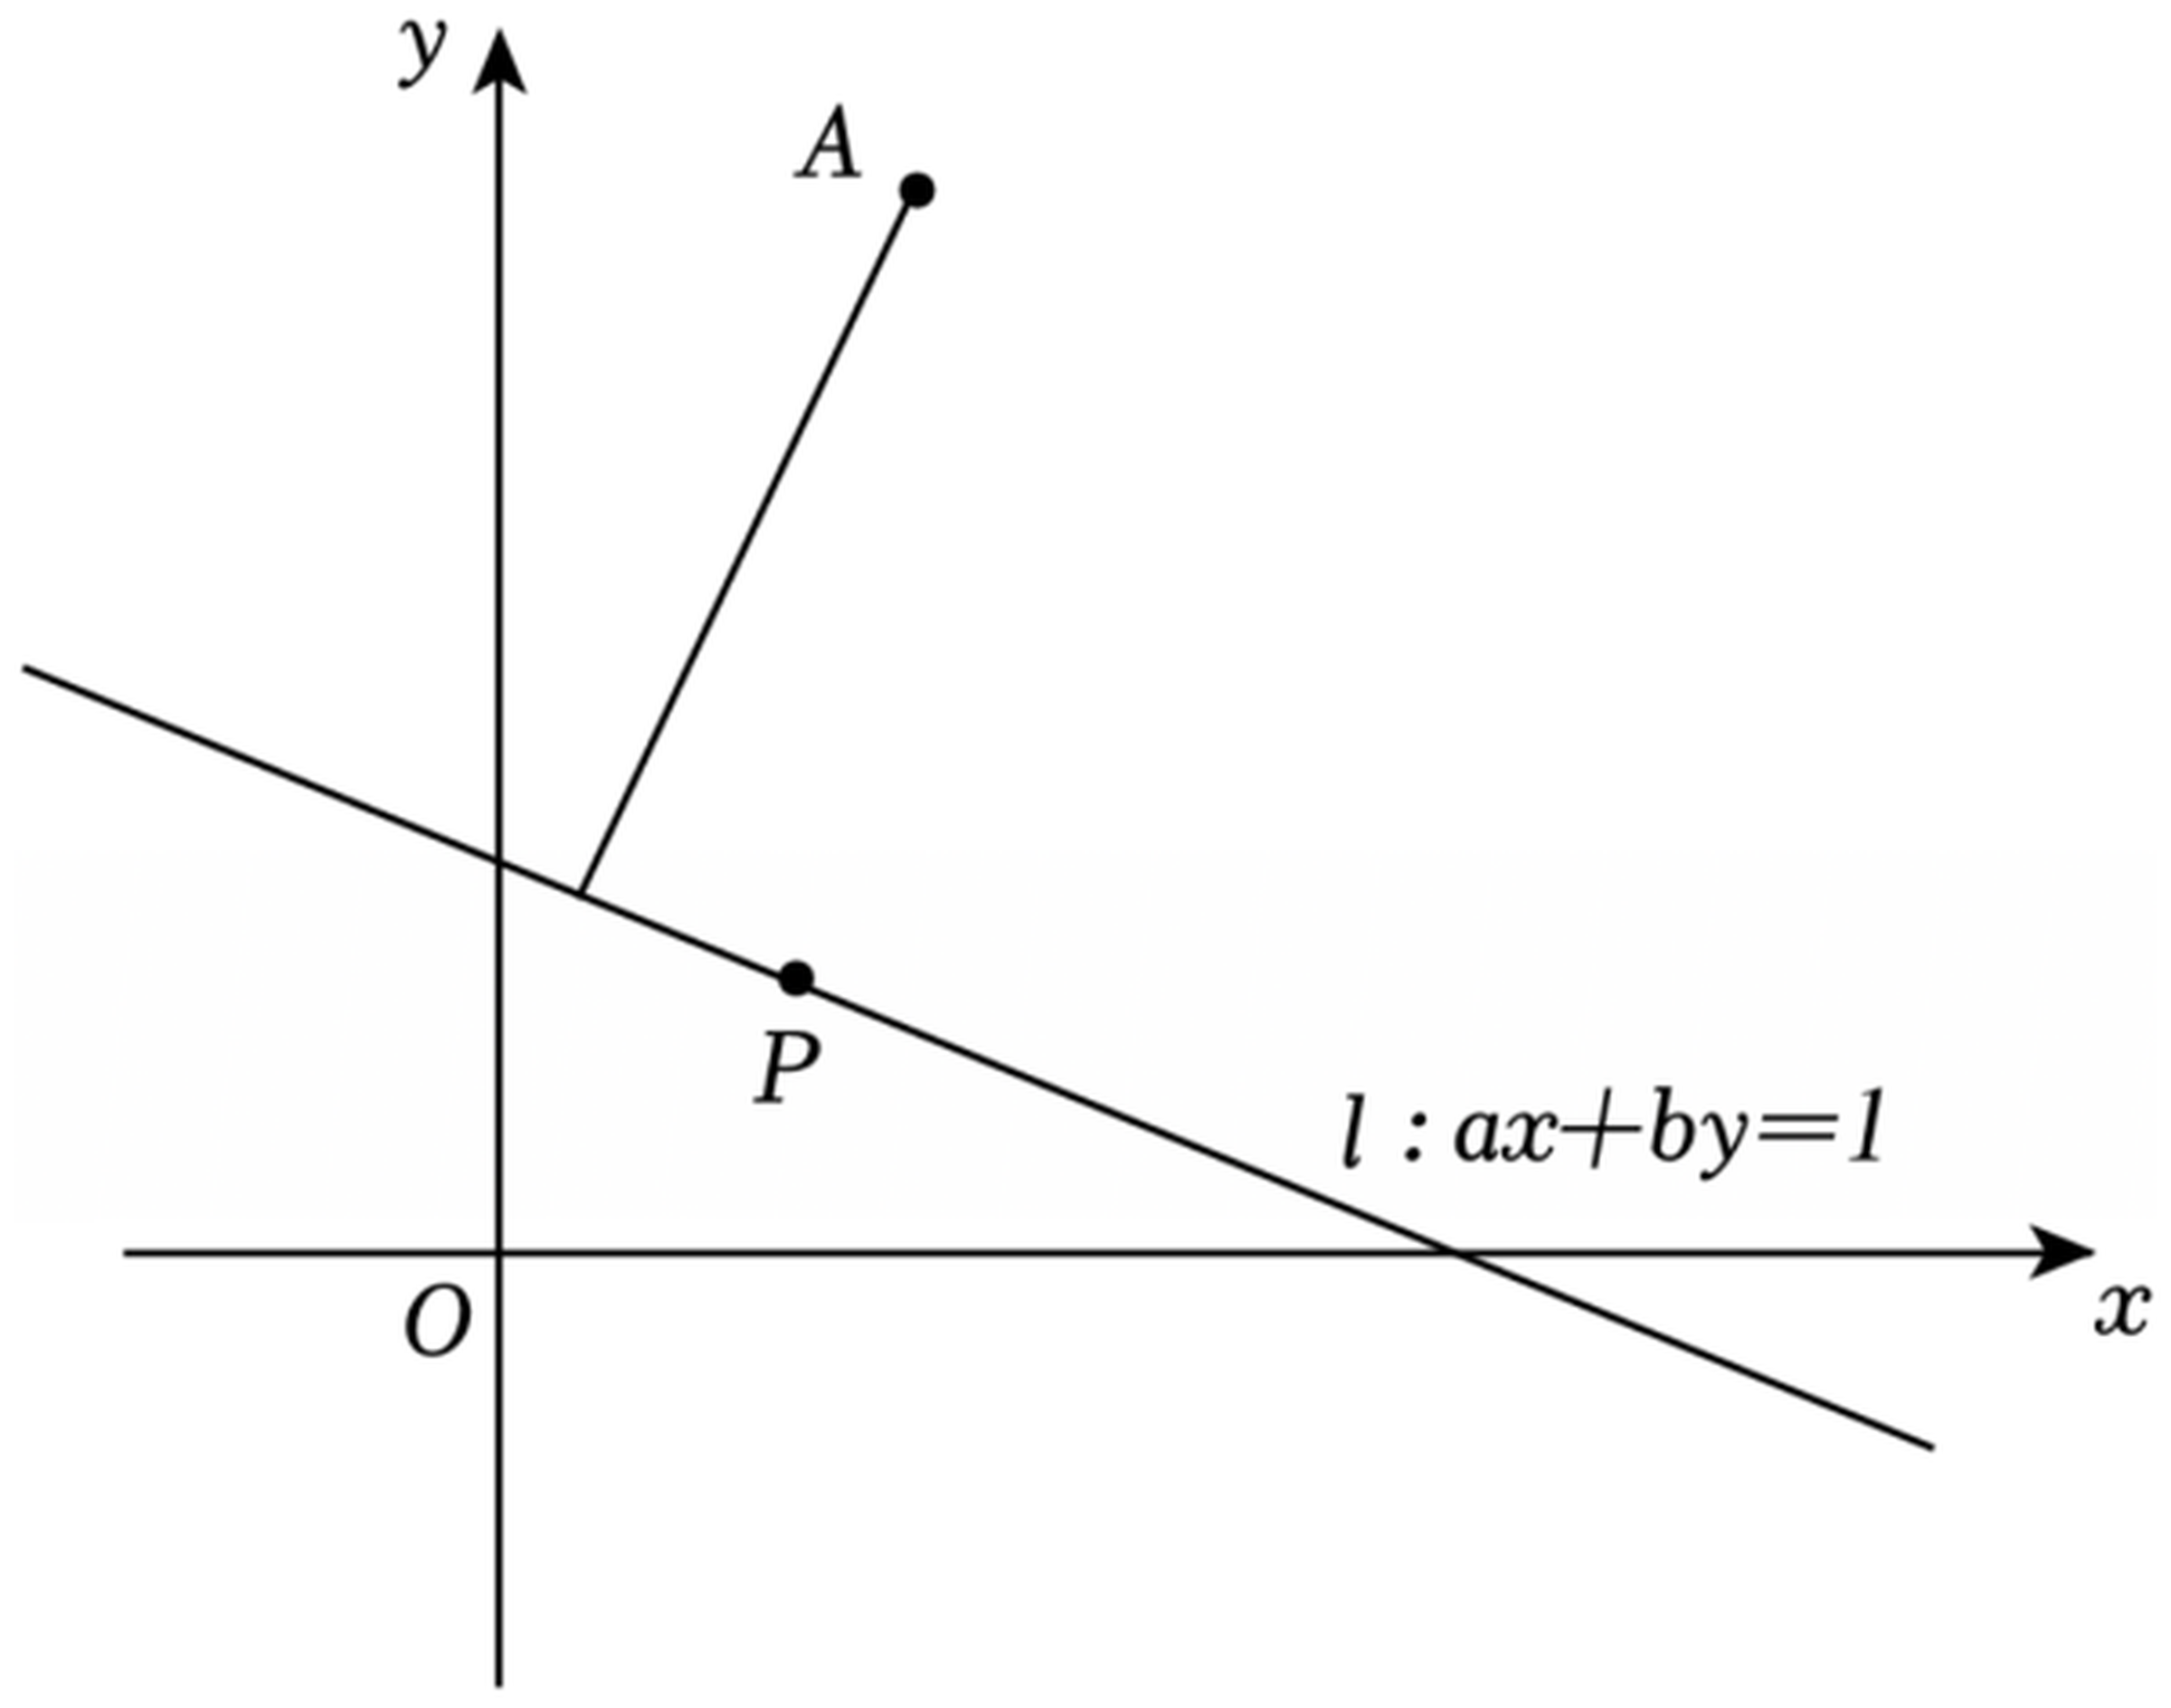
\includegraphics[width=0.56\textwidth]{figures/line_ax_plus_by_1.png}
\end{center}

\step{因为 $a+b=2$，所以直线 $l$ 恒过定点 $P\left(\dfrac12,\dfrac12\right)$，}
\step{再令 $A(1,2)$，则
$d_{A-l}=\dfrac{|a+2b-1|}{\sqrt{a^2+b^2}}\leqslant|AP|=\dfrac{\sqrt{10}}2$，}
\step{当且仅当 $l\perp AP$ 时等号成立，}
\step{又 $\dfrac{a+2b-1}{\sqrt{a^2+b^2}}\leqslant\dfrac{|a+2b-1|}{\sqrt{a^2+b^2}}$，
而当 $l\perp AP$，$a+2b-1>0$，等号也成立，}
\step{故 $\left(\dfrac{a+2b-1}{\sqrt{a^2+b^2}}\right)_{\max}=\dfrac{\sqrt{10}}2$.}
\solend

\fi

\ansspace[6]

\item （1）设 $a$、$b$、$c$ 都是正数，试证明不等式：
$\dfrac{b+c}a+\dfrac{c+a}b+\dfrac{a+b}c\geqslant6$；

（2）对一切正整数 $n$，不等式 $\dfrac{2x-1}x>\dfrac n{n+1}$ 恒成立，
则实数 $x$ 的取值范围构成的集合.

\ifanswer
\solbegin
\stepm{(1)}{因为 $a>0$，$b>0$，$c>0$，}
\step{所以 $\dfrac ba+\dfrac ab\geqslant2$，$\dfrac ca+\dfrac ac\geqslant2$，
$\dfrac cb+\dfrac bc\geqslant2$，}
\step{所以 $\left(\dfrac ba+\dfrac ab\right)+\left(\dfrac ca+\dfrac ac\right)
+\left(\dfrac cb+\dfrac bc\right)\geqslant6$，
即 $\dfrac{b+c}a+\dfrac{c+a}b+\dfrac{a+b}c\geqslant6$.}
% 注：下一行题干原卷作「……则实数 $x$ 的取值范围构成的集合.」，缺一个「求」字，
%     照抄未改，见文件头「原卷存疑」⑤。
\stepm{(2)}{考查 $y=\dfrac n{n+1}=1-\dfrac1{n+1}$，一切正整数 $n$ 函数为严格增函数，
所以 $y\geqslant\dfrac12$，}
\step{对一切正整数 $n$，不等式 $\dfrac{2x-1}x>\dfrac n{n+1}$ 恒成立，
所以 $\dfrac{2x-1}x\geqslant1$，}
\step{所以 $\dfrac{x-1}x\geqslant0$，所以 $x<0$ 或 $x\geqslant1$，}
\step{所以实数 $x$ 的取值范围是 $(-\infty,0)\cup[1,+\infty)$.}
\solend

\fi

\ansspace[6]

\end{enumerate}

\end{document}
"
%
% 原始材料是微信公众号图文（公众号「魔都数学加油站」连载「27学年高一 34」，2026-09-25 发布，
% 原文标题「27学年高一34——2026-2027年上海市交附闵行高一上查漏补缺卷」），
% 正文为 7 张 PNG 页（均 2560×3620），取 mmbiz.qpic.cn/<hash>/0 的原图档。
% 原文本身就是一份**讲评版**，但**全卷没有任何一处印「【答案】」**——每题下方直接印【解析】，
% 答案写在解析的末句。试题文字与解析均照原卷录入，未改内容。
% 卷面的粉色斜水印属水印，未录入。
%
% 卷首标题：原卷印作「2026-2027 年交附闵行高一上查漏补缺卷」（公众号标题里的「上海市」
% 三字卷面标题行没有，本稿照卷面），年份区间按全稿惯例排 en dash，前缀照原卷保留「年」。
%
% 与原卷的排版差异（均已在 README「说明」中交代）：
%   ① 原文自**第 3 题**起（第 1、2 题未在该文中发布），故本稿题号亦自 3 起；
%   ② 原卷只有「一、填空题」「二、解答题」两个节标题（本卷无选择题），本稿照原卷分节，
%      只把标题改排成全稿统一的「大节标题」样式；
%   ③ 原卷通篇只印【解析】（无【答案】行），本稿统一改为试卷版隐去、答案版以 \ifanswer{}
%      块给出，两版彻底分离；
%   ④ 数集记号原卷两套并用：第 4 题与第 11(2) 题作斜体的 $R$，第 7 题两处作粗体的
%      $\mathbf{R}^+$，本稿按全稿惯例统一写作 $\R$；
%   ⑤ 原卷填空的横线约两个字宽，本稿按全稿惯例统一排 \blankline[4.4em]（第 9 题的第一个空
%      原卷**没有**下划线、只留了一个空格，本稿仍补出横线，见文件头「原卷存疑」①）；
%   ⑥ 原卷未印副标题，本稿按全稿惯例补出副标题「集合与常用逻辑用语」（本卷实为基本不等式
%      专题，与 高一27／高一28 同样只标主章节，见文末「高一34 专记」）；
%   ⑦ 第 13 题的配图只出现在【解析】里（题干并未写「如图」），故放进 \ifanswer 块，
%      试卷版不排；图取原卷截图、4× LANCZOS 放大（figures/line_ax_plus_by_1.png）。
%
% 原卷存疑五处（均照抄原卷、未改，见源码中该处上方注释）：
%   ① 第 9 题「则 $ab$ 的最大值为 ，」——第一个空后面只有空格、没有下划线，第二个空才有；
%   ② 第 11(2) 题题干括号内写「$a$、$b\in R$」，但函数式 $f(x)=ax^2+(3a-4)x-12$ 里并没有 $b$；
%   ③ 第 10 题只限定 $a$ 是正实数，未提 $b$ 的取值范围；
%   ④ 第 13 题题干作「求 …… 的最大值为____.」（「求」与「为」混用），且**题干未写「如图」**，
%      是【解析】里才写「如图」；
%   ⑤ 第 14(2) 题题干作「……则实数 $x$ 的取值范围构成的集合.」——缺一个「求」字。
% 另有两处标点照录：第 9 题【解析】首句末是句号、第 11(1)① 解析末句是分号。

\documentclass[a4paper,11pt]{article}
\usepackage{common}

\begin{document}

\examtitlest[3]{2026--2027 年交附闵行高一上查漏补缺卷}{集合与常用逻辑用语}

\bigsec{一、填空题}

\begin{enumerate}
\setcounter{enumi}{2}

\item 已知正实数 $m$、$n$ 满足 $\dfrac1{m+2n}+\dfrac1{2m+n}=1$，则 $m+n$ 的最小值为
\blankline[4.4em].

\ifanswer
\solbegin
\step{因为 $m$、$n\in(0,+\infty)$，$\dfrac1{m+2n}+\dfrac1{2m+n}=1$，}
\step{所以 $m+n=\dfrac13[(m+2n)+(2m+n)]\left(\dfrac1{m+2n}+\dfrac1{2m+n}\right)$}
\step{$=\dfrac13\left[2+\dfrac{2m+n}{m+2n}+\dfrac{m+2n}{2m+n}\right]
\geqslant\dfrac13\left[2+2\sqrt{\dfrac{2m+n}{m+2n}\cdot\dfrac{m+2n}{2m+n}}\right]
=\dfrac43$，}
\step{当且仅当 $\dfrac{2m+n}{m+2n}=\dfrac{m+2n}{2m+n}$，即 $m=n=\dfrac23$ 时取等号，}
\step{所以 $m+n$ 的最小值为 $\dfrac43$.}
\solend

\fi

\item 若 $a$、$b\in\R$，且 $a^2+2ab-3b^2=1$，则 $a^2+b^2$ 的最小值为 \blankline[4.4em].

\ifanswer
\solbegin
\step{由 $a^2+2ab-3b^2=1$ 得 $(a+3b)(a-b)=1$，}
\step{令 $x=a+3b$，$y=a-b$，则 $xy=1$ 且 $a=\dfrac{x+3y}4$，$b=\dfrac{x-y}4$，}
\step{所以 $a^2+b^2=\left(\dfrac{x+3y}4\right)^2+\left(\dfrac{x-y}4\right)^2
=\dfrac{x^2+5y^2+2}8\geqslant\dfrac{2\sqrt{5x^2y^2}+2}8=\dfrac{\sqrt5+1}4$，}
\step{当且仅当 $x^2=\sqrt5$，$y^2=\dfrac{\sqrt5}5$ 时取等号，
故 $a^2+b^2$ 的最小值为 $\dfrac{\sqrt5+1}4$.}
\solend

\fi

\item 已知实数 $x$、$y$ 满足 $3x^2+3y^2-2xy=4$，则 $x+y$ 的最大值为 \blankline[4.4em].

\ifanswer
\solbegin
\step{由 $3x^2+3y^2-2xy=4$，则 $3[(x+y)^2-2xy]-2xy=4$，}
\step{设 $s=x+y$，则 $3s^2-8xy=4$，即 $xy=\dfrac{3s^2-4}8$，}
\step{对任意实数 $x$、$y$，有 $xy\leqslant\left(\dfrac{x+y}2\right)^2=\dfrac{s^2}4$，
即 $\dfrac{3s^2-4}8\leqslant\dfrac{s^2}4$，}
\step{得 $s^2\leqslant4$，即 $-2\leqslant s\leqslant2$，}
\step{当 $x=y=1$ 时，满足原等式，且 $x+y=2$ 成立，因此 $x+y$ 的最大值为 $2$.}
\solend

\fi

\item 若 $a$、$b$、$c$ 都是正实数，则 $\dfrac{a^2+2b^2+4c^2}{ab+2bc}$ 的最小值为
\blankline[4.4em].

\ifanswer
\solbegin
\step{因为 $a^2+2b^2+4c^2=a^2+b^2+b^2+4c^2=(a^2+b^2)+(b^2+4c^2)\geqslant2ab+4bc$，}
\step{所以 $\dfrac{a^2+2b^2+4c^2}{ab+2bc}\geqslant\dfrac{2ab+4bc}{ab+2bc}=2$，
当且仅当 $a=b=2c$ 时取等号，}
\step{即 $\dfrac{a^2+2b^2+4c^2}{ab+2bc}$ 的最小值是 $2$.}
\solend

\fi

\item 已知 $a$、$b\in\R^+$，且 $ab=2$，则 $\dfrac b{2+a^2}+\dfrac a{2+b^2}$ 的最小值是
\blankline[4.4em].

\ifanswer
\solbegin
\step{$\dfrac b{2+a^2}+\dfrac a{2+b^2}=\dfrac b{ab+a^2}+\dfrac a{ab+b^2}
=\dfrac b{a(a+b)}+\dfrac a{b(a+b)}$}
\step{$=\dfrac{(a+b)^2-4}{2(a+b)}=\dfrac{a+b}2-\dfrac2{a+b}$，}
\step{令 $t=a+b$，则原式可设为 $y=\dfrac t2-\dfrac2t$ 的函数，}
\step{当 $t>0$ 时，此函数为严格增函数，}
\step{因为 $a$、$b\in\R^+$ 且 $ab=2$，$t=a+b\geqslant2\sqrt{ab}=2\sqrt2$，}
\step{当且仅当 $a=b=\sqrt2$ 时，$t$ 的最小值为 $2\sqrt2$，}
\step{$y=\dfrac t2-\dfrac2t$ 在 $t\in[2\sqrt2,+\infty)$ 上严格增，}
\step{所以原式的最小值为 $\dfrac{2\sqrt2}2-\dfrac2{2\sqrt2}=\dfrac{\sqrt2}2$，
则 $\dfrac b{2+a^2}+\dfrac a{2+b^2}$ 的最小值是 $\dfrac{\sqrt2}2$.}
\solend

\fi

\item 设 $x$、$y$、$z$ 为正实数，满足 $x-2y+3z=0$，则 $\dfrac{y^2}{xz}$ 的最小值是
\blankline[4.4em].

\ifanswer
\solbegin
\step{因为 $x-2y+3z=0$，所以 $y=\dfrac{x+3z}2$，}
\step{所以 $\dfrac{y^2}{xz}=\dfrac{x^2+9z^2+6xz}{4xz}\geqslant\dfrac{6xz+6xz}{4xz}=3$，
当且仅当 $x=3z$ 时取等号，}
\step{故 $\dfrac{y^2}{xz}$ 的最小值是 $3$.}
\solend

\fi

% 注：下一题的第一个空原卷只留了一个空格、**没有**下划线（第二个空才有），本稿仍按全稿
%     惯例补出横线；另其【解析】首句末原卷作句号，照录。见文件头「原卷存疑」①。
\item 设 $a$、$b$ 为正实数，且 $a+b=3$，则 $ab$ 的最大值为 \blankline[4.4em]，
$\dfrac{a^2}{a+2}+\dfrac{b^2}{b+1}$ 的最小值为 \blankline[4.4em].

\ifanswer
\solbegin
\step{因为 $a>0$，$b>0$，所以 $a+b=3\geqslant2\sqrt{ab}$，}
\step{故 $ab$ 的最大值为 $\dfrac94$，当且仅当 $a=b=\dfrac32$ 时取等号.}
\step{令 $a+2=m$，$b+1=n$，则 $m+n=a+b+3=6$，}
\step{解得 $a=m-2$，$b=n-1$，}
\step{所以 $\dfrac{a^2}{a+2}+\dfrac{b^2}{b+1}=\dfrac{(m-2)^2}m+\dfrac{(n-1)^2}n
=m+\dfrac4m+n+\dfrac1n-6=\dfrac4m+\dfrac1n$}
\step{$=\dfrac16(m+n)\left(\dfrac4m+\dfrac1n\right)
=\dfrac16\left(\dfrac{4n}m+\dfrac mn+5\right)\geqslant\dfrac16(4+5)=\dfrac32$，}
\step{当且仅当 $\dfrac{4n}m=\dfrac mn$ 时，即 $m=2n$ 时
$\dfrac{a^2}{a+2}+\dfrac{b^2}{b+1}$ 取得最小值，}
\step{因此 $\dfrac{a^2}{a+2}+\dfrac{b^2}{b+1}$ 的最小值为 $\dfrac32$.}
\solend

\fi

\item 若 $a$ 是正实数，$2a^2+3b^2=10$，则 $a\sqrt{2+b^2}$ 的最大值是 \blankline[4.4em].

\ifanswer
\solbegin
\step{$a$ 是正实数，$2a^2+3b^2=10$，变形为 $2a^2+3(b^2+2)=16$，}
\step{所以 $16\geqslant2\sqrt{2a^2\times3(b^2+2)}=2\sqrt6\cdot a\sqrt{b^2+2}$，
得 $a\sqrt{2+b^2}\leqslant\dfrac{4\sqrt6}3$，}
\step{当且仅当 $2a^2=3(b^2+2)=8$，即 $a=2$，$b^2=\dfrac23$ 时取等号，}
\step{所以 $a\sqrt{2+b^2}$ 的最大值为 $\dfrac{4\sqrt6}3$.}
\solend

\fi

\end{enumerate}

\bigsec{二、解答题}

\begin{enumerate}
\setcounter{enumi}{10}

\item （1）已知 $x>0$，$y>0$，$2xy=x+4y$. ①求 $xy$ 的最小值；②求 $x+y$ 的最小值.

（2）已知函数 $f(x)=ax^2+(3a-4)x-12$（$a$、$b\in\R$），求不等式 $f(x)\geqslant0$ 的解集.

\ifanswer
\solbegin
\stepm{(1)}{①因为 $x>0$，$y>0$，由基本不等式得
$2xy=x+4y\geqslant2\sqrt{4xy}=4\sqrt{xy}$，}
\step{解得 $xy\geqslant4$，当且仅当 $x=4y=4$ 时取等号，故 $xy$ 的最小值为 $4$；}
\step{②因为 $x>0$，$y>0$，由已知条件得 $\dfrac{4y+x}{xy}=\dfrac4x+\dfrac1y=2$，}
\step{所以 $x+y=\dfrac12(x+y)\left(\dfrac4x+\dfrac1y\right)
=\dfrac12\left(5+\dfrac{4y}x+\dfrac xy\right)
\geqslant\dfrac12\left(5+2\sqrt{\dfrac{4y}x\cdot\dfrac xy}\right)=\dfrac92$，}
\step{当且仅当 $x=2y=3$ 时，等号成立，故 $x+y$ 的最小值为 $\dfrac92$；}
% 注：下一行题干括号内原卷写「$a$、$b\in R$」，但函数式里并没有 $b$，照抄未改，
%     见文件头「原卷存疑」②。
\stepm{(2)}{当 $a=0$ 时，则 $x+3\leqslant0$，解得 $x\leqslant-3$；}
\step{当 $a\neq0$ 时，$f(x)=ax^2+(3a-4)x-12=(x+3)(ax-4)
=a(x+3)\left(x-\dfrac4a\right)$，}
\step{当 $a>0$ 时，则 $(x+3)\left(x-\dfrac4a\right)\geqslant0$，
解得 $x\leqslant-3$ 或 $x\geqslant\dfrac4a$；}
\step{当 $a<0$ 时，则 $(x+3)\left(x-\dfrac4a\right)\leqslant0$，}
\step{当 $\dfrac4a>-3$ 时，即 $a<-\dfrac43$，解 $(x+3)\left(x-\dfrac4a\right)\leqslant0$，
得 $-3\leqslant x\leqslant\dfrac4a$；}
\step{当 $\dfrac4a=-3$ 时，即 $a=-\dfrac43$，解 $(x+3)\left(x-\dfrac4a\right)\leqslant0$，
得 $x=-3$；}
\step{当 $\dfrac4a<-3$ 时，即 $-\dfrac43<a<0$，解 $(x+3)\left(x-\dfrac4a\right)\leqslant0$，
得 $\dfrac4a\leqslant x\leqslant-3$；}
\step{综上所述，当 $a<-\dfrac43$ 时，不等式 $f(x)\geqslant0$ 的解集为
$\left[-3,\dfrac4a\right]$；}
\step{当 $a=-\dfrac43$ 时，不等式 $f(x)\geqslant0$ 的解集为 $\{-3\}$；}
\step{当 $-\dfrac43<a<0$ 时，不等式 $f(x)\geqslant0$ 的解集为
$\left[\dfrac4a,-3\right]$；}
\step{当 $a=0$ 时，不等式 $f(x)\geqslant0$ 的解集为 $(-\infty,-3]$；}
\step{当 $a>0$ 时，不等式 $f(x)\geqslant0$ 的解集为
$(-\infty,-3]\cup\left[\dfrac4a,+\infty\right)$.}
\solend

\fi

\ansspace[8]

\item 已知 $x$、$y$ 都是正数，且 $\dfrac2x+\dfrac1y=1$.

\begin{enumerate}[label=(\arabic*)]
\item 求 $2x+y$ 的最小值及此时 $x$、$y$ 的取值；
\item 不等式 $(2x+y)^2\geqslant m(x+2y)$ 恒成立，求实数 $m$ 的取值范围.
\end{enumerate}

\ifanswer
\solbegin
\stepm{(1)}{$2x+y=(2x+y)\left(\dfrac2x+\dfrac1y\right)
=4+\dfrac{2x}y+\dfrac{2y}x+1\geqslant5+2\sqrt{\dfrac{2x}y\cdot\dfrac{2y}x}=9$，}
\step{当且仅当 $x=y$ 且 $\dfrac2x+\dfrac1y=1$，即 $x=y=3$ 时取等号，}
\step{此时 $2x+y$ 的最小值为 $9$.}
\stepm{(2)}{由 $\dfrac2x+\dfrac1y=1$，得 $x+2y=xy>0$，}
\step{故 $(2x+y)^2\geqslant m(x+2y)\Leftrightarrow m\leqslant\dfrac{(2x+y)^2}{x+2y}
\Leftrightarrow m\leqslant\dfrac{(2x+y)^2}{xy}$，}
\step{又 $\dfrac{(2x+y)^2}{xy}=\dfrac{4x^2+y^2+4xy}{xy}
=\dfrac{4x}y+\dfrac yx+4\geqslant2\sqrt{\dfrac{4x}y\cdot\dfrac yx}+4=8$，}
\step{当且仅当 $\begin{cases}\dfrac{4x}y=\dfrac yx\\[2pt]
\dfrac2x+\dfrac1y=1\end{cases}$ 时取等号，$\dfrac{(2x+y)^2}{xy}$ 取得最小值 $8$，}
\step{故 $m$ 的取值范围为 $\{m\mid m\leqslant8\}$.}
\solend

\fi

\ansspace[6]

% 注：本小题题干作「求 …… 的最大值为____.」（「求」与「为」混用），且**题干未写「如图」**
%     ——是【解析】里才写「如图」，照抄未改，见文件头「原卷存疑」④。
\item 已知实数 $a$、$b$ 满足 $a+b=2$，求 $\dfrac{a+2b-1}{\sqrt{a^2+b^2}}$ 的最大值为
\blankline[4.4em].

\ifanswer
\solbegin
\step{如图，考虑直线 $l:ax+by=1$，}

\begin{center}
% 图取原卷截图、4× LANCZOS 放大。图只在【解析】里出现（题干并未写「如图」），
% 故放进 \ifanswer 块，试卷版不排，见文件头⑦。
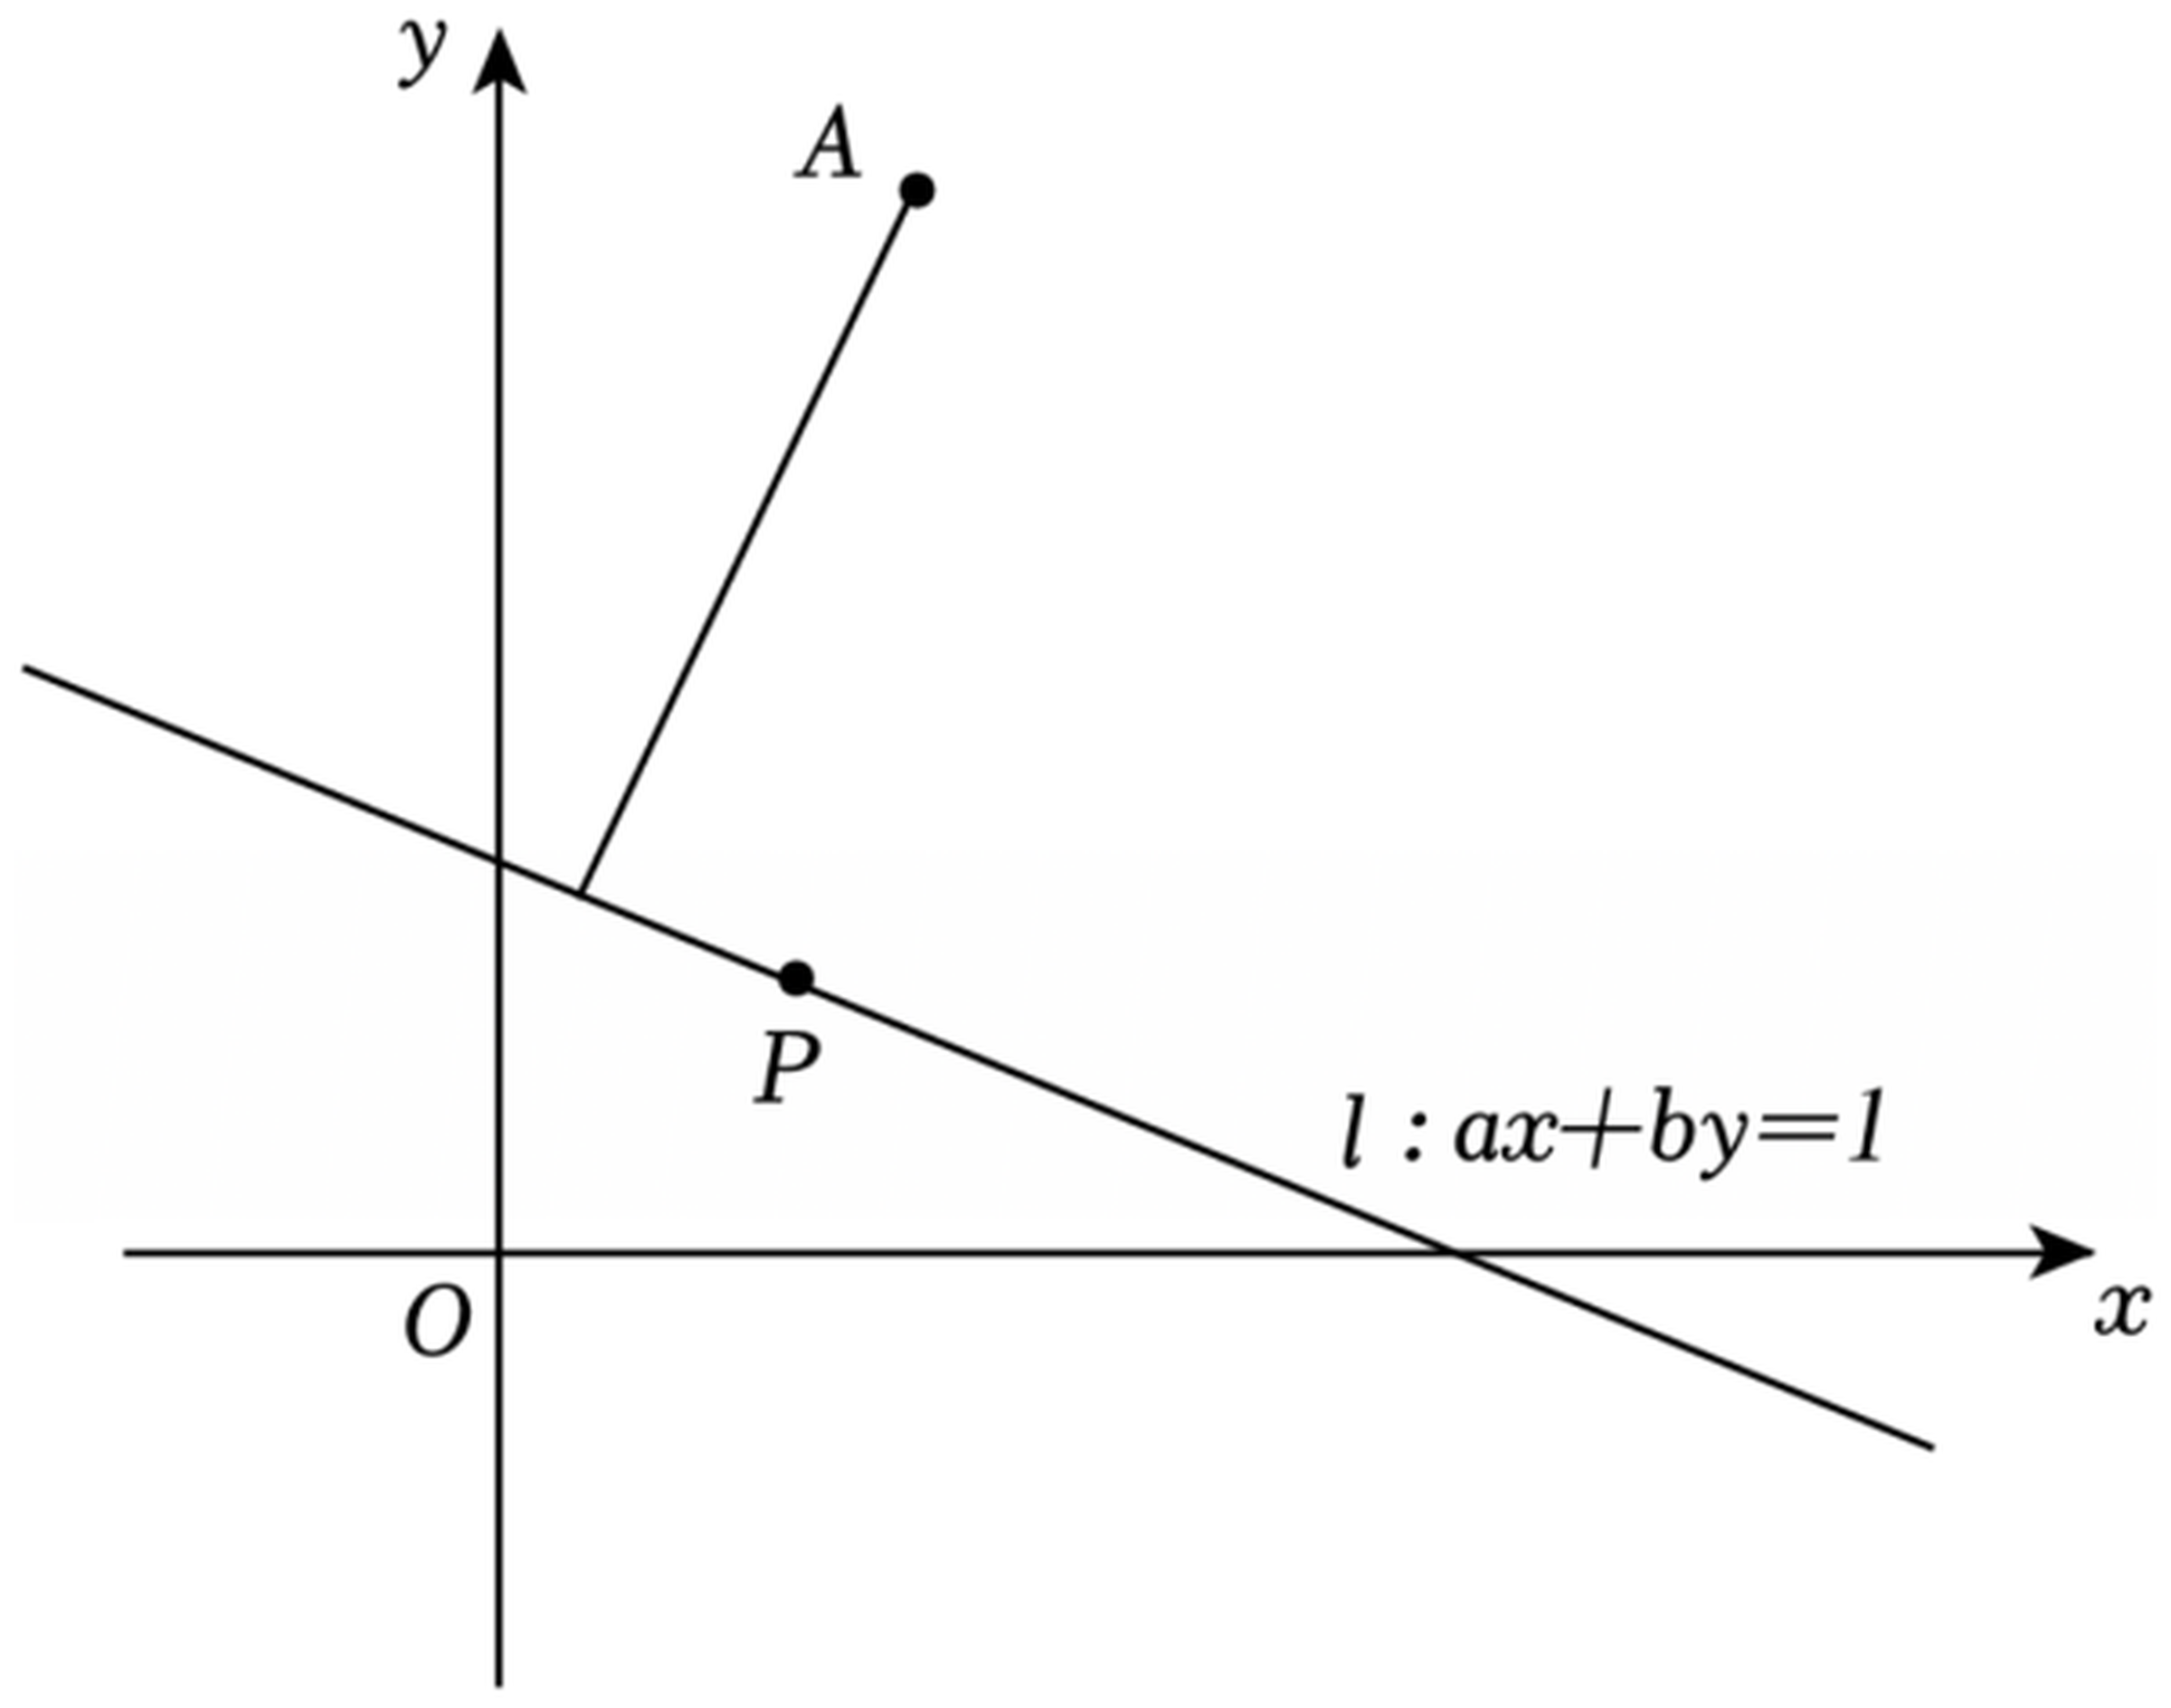
\includegraphics[width=0.56\textwidth]{figures/line_ax_plus_by_1.png}
\end{center}

\step{因为 $a+b=2$，所以直线 $l$ 恒过定点 $P\left(\dfrac12,\dfrac12\right)$，}
\step{再令 $A(1,2)$，则
$d_{A-l}=\dfrac{|a+2b-1|}{\sqrt{a^2+b^2}}\leqslant|AP|=\dfrac{\sqrt{10}}2$，}
\step{当且仅当 $l\perp AP$ 时等号成立，}
\step{又 $\dfrac{a+2b-1}{\sqrt{a^2+b^2}}\leqslant\dfrac{|a+2b-1|}{\sqrt{a^2+b^2}}$，
而当 $l\perp AP$，$a+2b-1>0$，等号也成立，}
\step{故 $\left(\dfrac{a+2b-1}{\sqrt{a^2+b^2}}\right)_{\max}=\dfrac{\sqrt{10}}2$.}
\solend

\fi

\ansspace[6]

\item （1）设 $a$、$b$、$c$ 都是正数，试证明不等式：
$\dfrac{b+c}a+\dfrac{c+a}b+\dfrac{a+b}c\geqslant6$；

（2）对一切正整数 $n$，不等式 $\dfrac{2x-1}x>\dfrac n{n+1}$ 恒成立，
则实数 $x$ 的取值范围构成的集合.

\ifanswer
\solbegin
\stepm{(1)}{因为 $a>0$，$b>0$，$c>0$，}
\step{所以 $\dfrac ba+\dfrac ab\geqslant2$，$\dfrac ca+\dfrac ac\geqslant2$，
$\dfrac cb+\dfrac bc\geqslant2$，}
\step{所以 $\left(\dfrac ba+\dfrac ab\right)+\left(\dfrac ca+\dfrac ac\right)
+\left(\dfrac cb+\dfrac bc\right)\geqslant6$，
即 $\dfrac{b+c}a+\dfrac{c+a}b+\dfrac{a+b}c\geqslant6$.}
% 注：下一行题干原卷作「……则实数 $x$ 的取值范围构成的集合.」，缺一个「求」字，
%     照抄未改，见文件头「原卷存疑」⑤。
\stepm{(2)}{考查 $y=\dfrac n{n+1}=1-\dfrac1{n+1}$，一切正整数 $n$ 函数为严格增函数，
所以 $y\geqslant\dfrac12$，}
\step{对一切正整数 $n$，不等式 $\dfrac{2x-1}x>\dfrac n{n+1}$ 恒成立，
所以 $\dfrac{2x-1}x\geqslant1$，}
\step{所以 $\dfrac{x-1}x\geqslant0$，所以 $x<0$ 或 $x\geqslant1$，}
\step{所以实数 $x$ 的取值范围是 $(-\infty,0)\cup[1,+\infty)$.}
\solend

\fi

\ansspace[6]

\end{enumerate}

\end{document}
"
% 紧凑版：xelatex "\def\iscompact{1}% 高一34_交附闵行_查漏补缺卷.tex
%   —— 高一上数学「2026-2027 年交附闵行高一上查漏补缺卷」（试卷版/答案版）
% 试卷版：xelatex 高一34_交附闵行_查漏补缺卷.tex
% 答案版：xelatex "\def\isanswer{1}% 高一34_交附闵行_查漏补缺卷.tex
%   —— 高一上数学「2026-2027 年交附闵行高一上查漏补缺卷」（试卷版/答案版）
% 试卷版：xelatex 高一34_交附闵行_查漏补缺卷.tex
% 答案版：xelatex "\def\isanswer{1}% 高一34_交附闵行_查漏补缺卷.tex
%   —— 高一上数学「2026-2027 年交附闵行高一上查漏补缺卷」（试卷版/答案版）
% 试卷版：xelatex 高一34_交附闵行_查漏补缺卷.tex
% 答案版：xelatex "\def\isanswer{1}\input{高一34_交附闵行_查漏补缺卷.tex}"
% 紧凑版：xelatex "\def\iscompact{1}\input{高一34_交附闵行_查漏补缺卷.tex}"
%
% 原始材料是微信公众号图文（公众号「魔都数学加油站」连载「27学年高一 34」，2026-09-25 发布，
% 原文标题「27学年高一34——2026-2027年上海市交附闵行高一上查漏补缺卷」），
% 正文为 7 张 PNG 页（均 2560×3620），取 mmbiz.qpic.cn/<hash>/0 的原图档。
% 原文本身就是一份**讲评版**，但**全卷没有任何一处印「【答案】」**——每题下方直接印【解析】，
% 答案写在解析的末句。试题文字与解析均照原卷录入，未改内容。
% 卷面的粉色斜水印属水印，未录入。
%
% 卷首标题：原卷印作「2026-2027 年交附闵行高一上查漏补缺卷」（公众号标题里的「上海市」
% 三字卷面标题行没有，本稿照卷面），年份区间按全稿惯例排 en dash，前缀照原卷保留「年」。
%
% 与原卷的排版差异（均已在 README「说明」中交代）：
%   ① 原文自**第 3 题**起（第 1、2 题未在该文中发布），故本稿题号亦自 3 起；
%   ② 原卷只有「一、填空题」「二、解答题」两个节标题（本卷无选择题），本稿照原卷分节，
%      只把标题改排成全稿统一的「大节标题」样式；
%   ③ 原卷通篇只印【解析】（无【答案】行），本稿统一改为试卷版隐去、答案版以 \ifanswer{}
%      块给出，两版彻底分离；
%   ④ 数集记号原卷两套并用：第 4 题与第 11(2) 题作斜体的 $R$，第 7 题两处作粗体的
%      $\mathbf{R}^+$，本稿按全稿惯例统一写作 $\R$；
%   ⑤ 原卷填空的横线约两个字宽，本稿按全稿惯例统一排 \blankline[4.4em]（第 9 题的第一个空
%      原卷**没有**下划线、只留了一个空格，本稿仍补出横线，见文件头「原卷存疑」①）；
%   ⑥ 原卷未印副标题，本稿按全稿惯例补出副标题「集合与常用逻辑用语」（本卷实为基本不等式
%      专题，与 高一27／高一28 同样只标主章节，见文末「高一34 专记」）；
%   ⑦ 第 13 题的配图只出现在【解析】里（题干并未写「如图」），故放进 \ifanswer 块，
%      试卷版不排；图取原卷截图、4× LANCZOS 放大（figures/line_ax_plus_by_1.png）。
%
% 原卷存疑五处（均照抄原卷、未改，见源码中该处上方注释）：
%   ① 第 9 题「则 $ab$ 的最大值为 ，」——第一个空后面只有空格、没有下划线，第二个空才有；
%   ② 第 11(2) 题题干括号内写「$a$、$b\in R$」，但函数式 $f(x)=ax^2+(3a-4)x-12$ 里并没有 $b$；
%   ③ 第 10 题只限定 $a$ 是正实数，未提 $b$ 的取值范围；
%   ④ 第 13 题题干作「求 …… 的最大值为____.」（「求」与「为」混用），且**题干未写「如图」**，
%      是【解析】里才写「如图」；
%   ⑤ 第 14(2) 题题干作「……则实数 $x$ 的取值范围构成的集合.」——缺一个「求」字。
% 另有两处标点照录：第 9 题【解析】首句末是句号、第 11(1)① 解析末句是分号。

\documentclass[a4paper,11pt]{article}
\usepackage{common}

\begin{document}

\examtitlest[3]{2026--2027 年交附闵行高一上查漏补缺卷}{集合与常用逻辑用语}

\bigsec{一、填空题}

\begin{enumerate}
\setcounter{enumi}{2}

\item 已知正实数 $m$、$n$ 满足 $\dfrac1{m+2n}+\dfrac1{2m+n}=1$，则 $m+n$ 的最小值为
\blankline[4.4em].

\ifanswer
\solbegin
\step{因为 $m$、$n\in(0,+\infty)$，$\dfrac1{m+2n}+\dfrac1{2m+n}=1$，}
\step{所以 $m+n=\dfrac13[(m+2n)+(2m+n)]\left(\dfrac1{m+2n}+\dfrac1{2m+n}\right)$}
\step{$=\dfrac13\left[2+\dfrac{2m+n}{m+2n}+\dfrac{m+2n}{2m+n}\right]
\geqslant\dfrac13\left[2+2\sqrt{\dfrac{2m+n}{m+2n}\cdot\dfrac{m+2n}{2m+n}}\right]
=\dfrac43$，}
\step{当且仅当 $\dfrac{2m+n}{m+2n}=\dfrac{m+2n}{2m+n}$，即 $m=n=\dfrac23$ 时取等号，}
\step{所以 $m+n$ 的最小值为 $\dfrac43$.}
\solend

\fi

\item 若 $a$、$b\in\R$，且 $a^2+2ab-3b^2=1$，则 $a^2+b^2$ 的最小值为 \blankline[4.4em].

\ifanswer
\solbegin
\step{由 $a^2+2ab-3b^2=1$ 得 $(a+3b)(a-b)=1$，}
\step{令 $x=a+3b$，$y=a-b$，则 $xy=1$ 且 $a=\dfrac{x+3y}4$，$b=\dfrac{x-y}4$，}
\step{所以 $a^2+b^2=\left(\dfrac{x+3y}4\right)^2+\left(\dfrac{x-y}4\right)^2
=\dfrac{x^2+5y^2+2}8\geqslant\dfrac{2\sqrt{5x^2y^2}+2}8=\dfrac{\sqrt5+1}4$，}
\step{当且仅当 $x^2=\sqrt5$，$y^2=\dfrac{\sqrt5}5$ 时取等号，
故 $a^2+b^2$ 的最小值为 $\dfrac{\sqrt5+1}4$.}
\solend

\fi

\item 已知实数 $x$、$y$ 满足 $3x^2+3y^2-2xy=4$，则 $x+y$ 的最大值为 \blankline[4.4em].

\ifanswer
\solbegin
\step{由 $3x^2+3y^2-2xy=4$，则 $3[(x+y)^2-2xy]-2xy=4$，}
\step{设 $s=x+y$，则 $3s^2-8xy=4$，即 $xy=\dfrac{3s^2-4}8$，}
\step{对任意实数 $x$、$y$，有 $xy\leqslant\left(\dfrac{x+y}2\right)^2=\dfrac{s^2}4$，
即 $\dfrac{3s^2-4}8\leqslant\dfrac{s^2}4$，}
\step{得 $s^2\leqslant4$，即 $-2\leqslant s\leqslant2$，}
\step{当 $x=y=1$ 时，满足原等式，且 $x+y=2$ 成立，因此 $x+y$ 的最大值为 $2$.}
\solend

\fi

\item 若 $a$、$b$、$c$ 都是正实数，则 $\dfrac{a^2+2b^2+4c^2}{ab+2bc}$ 的最小值为
\blankline[4.4em].

\ifanswer
\solbegin
\step{因为 $a^2+2b^2+4c^2=a^2+b^2+b^2+4c^2=(a^2+b^2)+(b^2+4c^2)\geqslant2ab+4bc$，}
\step{所以 $\dfrac{a^2+2b^2+4c^2}{ab+2bc}\geqslant\dfrac{2ab+4bc}{ab+2bc}=2$，
当且仅当 $a=b=2c$ 时取等号，}
\step{即 $\dfrac{a^2+2b^2+4c^2}{ab+2bc}$ 的最小值是 $2$.}
\solend

\fi

\item 已知 $a$、$b\in\R^+$，且 $ab=2$，则 $\dfrac b{2+a^2}+\dfrac a{2+b^2}$ 的最小值是
\blankline[4.4em].

\ifanswer
\solbegin
\step{$\dfrac b{2+a^2}+\dfrac a{2+b^2}=\dfrac b{ab+a^2}+\dfrac a{ab+b^2}
=\dfrac b{a(a+b)}+\dfrac a{b(a+b)}$}
\step{$=\dfrac{(a+b)^2-4}{2(a+b)}=\dfrac{a+b}2-\dfrac2{a+b}$，}
\step{令 $t=a+b$，则原式可设为 $y=\dfrac t2-\dfrac2t$ 的函数，}
\step{当 $t>0$ 时，此函数为严格增函数，}
\step{因为 $a$、$b\in\R^+$ 且 $ab=2$，$t=a+b\geqslant2\sqrt{ab}=2\sqrt2$，}
\step{当且仅当 $a=b=\sqrt2$ 时，$t$ 的最小值为 $2\sqrt2$，}
\step{$y=\dfrac t2-\dfrac2t$ 在 $t\in[2\sqrt2,+\infty)$ 上严格增，}
\step{所以原式的最小值为 $\dfrac{2\sqrt2}2-\dfrac2{2\sqrt2}=\dfrac{\sqrt2}2$，
则 $\dfrac b{2+a^2}+\dfrac a{2+b^2}$ 的最小值是 $\dfrac{\sqrt2}2$.}
\solend

\fi

\item 设 $x$、$y$、$z$ 为正实数，满足 $x-2y+3z=0$，则 $\dfrac{y^2}{xz}$ 的最小值是
\blankline[4.4em].

\ifanswer
\solbegin
\step{因为 $x-2y+3z=0$，所以 $y=\dfrac{x+3z}2$，}
\step{所以 $\dfrac{y^2}{xz}=\dfrac{x^2+9z^2+6xz}{4xz}\geqslant\dfrac{6xz+6xz}{4xz}=3$，
当且仅当 $x=3z$ 时取等号，}
\step{故 $\dfrac{y^2}{xz}$ 的最小值是 $3$.}
\solend

\fi

% 注：下一题的第一个空原卷只留了一个空格、**没有**下划线（第二个空才有），本稿仍按全稿
%     惯例补出横线；另其【解析】首句末原卷作句号，照录。见文件头「原卷存疑」①。
\item 设 $a$、$b$ 为正实数，且 $a+b=3$，则 $ab$ 的最大值为 \blankline[4.4em]，
$\dfrac{a^2}{a+2}+\dfrac{b^2}{b+1}$ 的最小值为 \blankline[4.4em].

\ifanswer
\solbegin
\step{因为 $a>0$，$b>0$，所以 $a+b=3\geqslant2\sqrt{ab}$，}
\step{故 $ab$ 的最大值为 $\dfrac94$，当且仅当 $a=b=\dfrac32$ 时取等号.}
\step{令 $a+2=m$，$b+1=n$，则 $m+n=a+b+3=6$，}
\step{解得 $a=m-2$，$b=n-1$，}
\step{所以 $\dfrac{a^2}{a+2}+\dfrac{b^2}{b+1}=\dfrac{(m-2)^2}m+\dfrac{(n-1)^2}n
=m+\dfrac4m+n+\dfrac1n-6=\dfrac4m+\dfrac1n$}
\step{$=\dfrac16(m+n)\left(\dfrac4m+\dfrac1n\right)
=\dfrac16\left(\dfrac{4n}m+\dfrac mn+5\right)\geqslant\dfrac16(4+5)=\dfrac32$，}
\step{当且仅当 $\dfrac{4n}m=\dfrac mn$ 时，即 $m=2n$ 时
$\dfrac{a^2}{a+2}+\dfrac{b^2}{b+1}$ 取得最小值，}
\step{因此 $\dfrac{a^2}{a+2}+\dfrac{b^2}{b+1}$ 的最小值为 $\dfrac32$.}
\solend

\fi

\item 若 $a$ 是正实数，$2a^2+3b^2=10$，则 $a\sqrt{2+b^2}$ 的最大值是 \blankline[4.4em].

\ifanswer
\solbegin
\step{$a$ 是正实数，$2a^2+3b^2=10$，变形为 $2a^2+3(b^2+2)=16$，}
\step{所以 $16\geqslant2\sqrt{2a^2\times3(b^2+2)}=2\sqrt6\cdot a\sqrt{b^2+2}$，
得 $a\sqrt{2+b^2}\leqslant\dfrac{4\sqrt6}3$，}
\step{当且仅当 $2a^2=3(b^2+2)=8$，即 $a=2$，$b^2=\dfrac23$ 时取等号，}
\step{所以 $a\sqrt{2+b^2}$ 的最大值为 $\dfrac{4\sqrt6}3$.}
\solend

\fi

\end{enumerate}

\bigsec{二、解答题}

\begin{enumerate}
\setcounter{enumi}{10}

\item （1）已知 $x>0$，$y>0$，$2xy=x+4y$. ①求 $xy$ 的最小值；②求 $x+y$ 的最小值.

（2）已知函数 $f(x)=ax^2+(3a-4)x-12$（$a$、$b\in\R$），求不等式 $f(x)\geqslant0$ 的解集.

\ifanswer
\solbegin
\stepm{(1)}{①因为 $x>0$，$y>0$，由基本不等式得
$2xy=x+4y\geqslant2\sqrt{4xy}=4\sqrt{xy}$，}
\step{解得 $xy\geqslant4$，当且仅当 $x=4y=4$ 时取等号，故 $xy$ 的最小值为 $4$；}
\step{②因为 $x>0$，$y>0$，由已知条件得 $\dfrac{4y+x}{xy}=\dfrac4x+\dfrac1y=2$，}
\step{所以 $x+y=\dfrac12(x+y)\left(\dfrac4x+\dfrac1y\right)
=\dfrac12\left(5+\dfrac{4y}x+\dfrac xy\right)
\geqslant\dfrac12\left(5+2\sqrt{\dfrac{4y}x\cdot\dfrac xy}\right)=\dfrac92$，}
\step{当且仅当 $x=2y=3$ 时，等号成立，故 $x+y$ 的最小值为 $\dfrac92$；}
% 注：下一行题干括号内原卷写「$a$、$b\in R$」，但函数式里并没有 $b$，照抄未改，
%     见文件头「原卷存疑」②。
\stepm{(2)}{当 $a=0$ 时，则 $x+3\leqslant0$，解得 $x\leqslant-3$；}
\step{当 $a\neq0$ 时，$f(x)=ax^2+(3a-4)x-12=(x+3)(ax-4)
=a(x+3)\left(x-\dfrac4a\right)$，}
\step{当 $a>0$ 时，则 $(x+3)\left(x-\dfrac4a\right)\geqslant0$，
解得 $x\leqslant-3$ 或 $x\geqslant\dfrac4a$；}
\step{当 $a<0$ 时，则 $(x+3)\left(x-\dfrac4a\right)\leqslant0$，}
\step{当 $\dfrac4a>-3$ 时，即 $a<-\dfrac43$，解 $(x+3)\left(x-\dfrac4a\right)\leqslant0$，
得 $-3\leqslant x\leqslant\dfrac4a$；}
\step{当 $\dfrac4a=-3$ 时，即 $a=-\dfrac43$，解 $(x+3)\left(x-\dfrac4a\right)\leqslant0$，
得 $x=-3$；}
\step{当 $\dfrac4a<-3$ 时，即 $-\dfrac43<a<0$，解 $(x+3)\left(x-\dfrac4a\right)\leqslant0$，
得 $\dfrac4a\leqslant x\leqslant-3$；}
\step{综上所述，当 $a<-\dfrac43$ 时，不等式 $f(x)\geqslant0$ 的解集为
$\left[-3,\dfrac4a\right]$；}
\step{当 $a=-\dfrac43$ 时，不等式 $f(x)\geqslant0$ 的解集为 $\{-3\}$；}
\step{当 $-\dfrac43<a<0$ 时，不等式 $f(x)\geqslant0$ 的解集为
$\left[\dfrac4a,-3\right]$；}
\step{当 $a=0$ 时，不等式 $f(x)\geqslant0$ 的解集为 $(-\infty,-3]$；}
\step{当 $a>0$ 时，不等式 $f(x)\geqslant0$ 的解集为
$(-\infty,-3]\cup\left[\dfrac4a,+\infty\right)$.}
\solend

\fi

\ansspace[8]

\item 已知 $x$、$y$ 都是正数，且 $\dfrac2x+\dfrac1y=1$.

\begin{enumerate}[label=(\arabic*)]
\item 求 $2x+y$ 的最小值及此时 $x$、$y$ 的取值；
\item 不等式 $(2x+y)^2\geqslant m(x+2y)$ 恒成立，求实数 $m$ 的取值范围.
\end{enumerate}

\ifanswer
\solbegin
\stepm{(1)}{$2x+y=(2x+y)\left(\dfrac2x+\dfrac1y\right)
=4+\dfrac{2x}y+\dfrac{2y}x+1\geqslant5+2\sqrt{\dfrac{2x}y\cdot\dfrac{2y}x}=9$，}
\step{当且仅当 $x=y$ 且 $\dfrac2x+\dfrac1y=1$，即 $x=y=3$ 时取等号，}
\step{此时 $2x+y$ 的最小值为 $9$.}
\stepm{(2)}{由 $\dfrac2x+\dfrac1y=1$，得 $x+2y=xy>0$，}
\step{故 $(2x+y)^2\geqslant m(x+2y)\Leftrightarrow m\leqslant\dfrac{(2x+y)^2}{x+2y}
\Leftrightarrow m\leqslant\dfrac{(2x+y)^2}{xy}$，}
\step{又 $\dfrac{(2x+y)^2}{xy}=\dfrac{4x^2+y^2+4xy}{xy}
=\dfrac{4x}y+\dfrac yx+4\geqslant2\sqrt{\dfrac{4x}y\cdot\dfrac yx}+4=8$，}
\step{当且仅当 $\begin{cases}\dfrac{4x}y=\dfrac yx\\[2pt]
\dfrac2x+\dfrac1y=1\end{cases}$ 时取等号，$\dfrac{(2x+y)^2}{xy}$ 取得最小值 $8$，}
\step{故 $m$ 的取值范围为 $\{m\mid m\leqslant8\}$.}
\solend

\fi

\ansspace[6]

% 注：本小题题干作「求 …… 的最大值为____.」（「求」与「为」混用），且**题干未写「如图」**
%     ——是【解析】里才写「如图」，照抄未改，见文件头「原卷存疑」④。
\item 已知实数 $a$、$b$ 满足 $a+b=2$，求 $\dfrac{a+2b-1}{\sqrt{a^2+b^2}}$ 的最大值为
\blankline[4.4em].

\ifanswer
\solbegin
\step{如图，考虑直线 $l:ax+by=1$，}

\begin{center}
% 图取原卷截图、4× LANCZOS 放大。图只在【解析】里出现（题干并未写「如图」），
% 故放进 \ifanswer 块，试卷版不排，见文件头⑦。
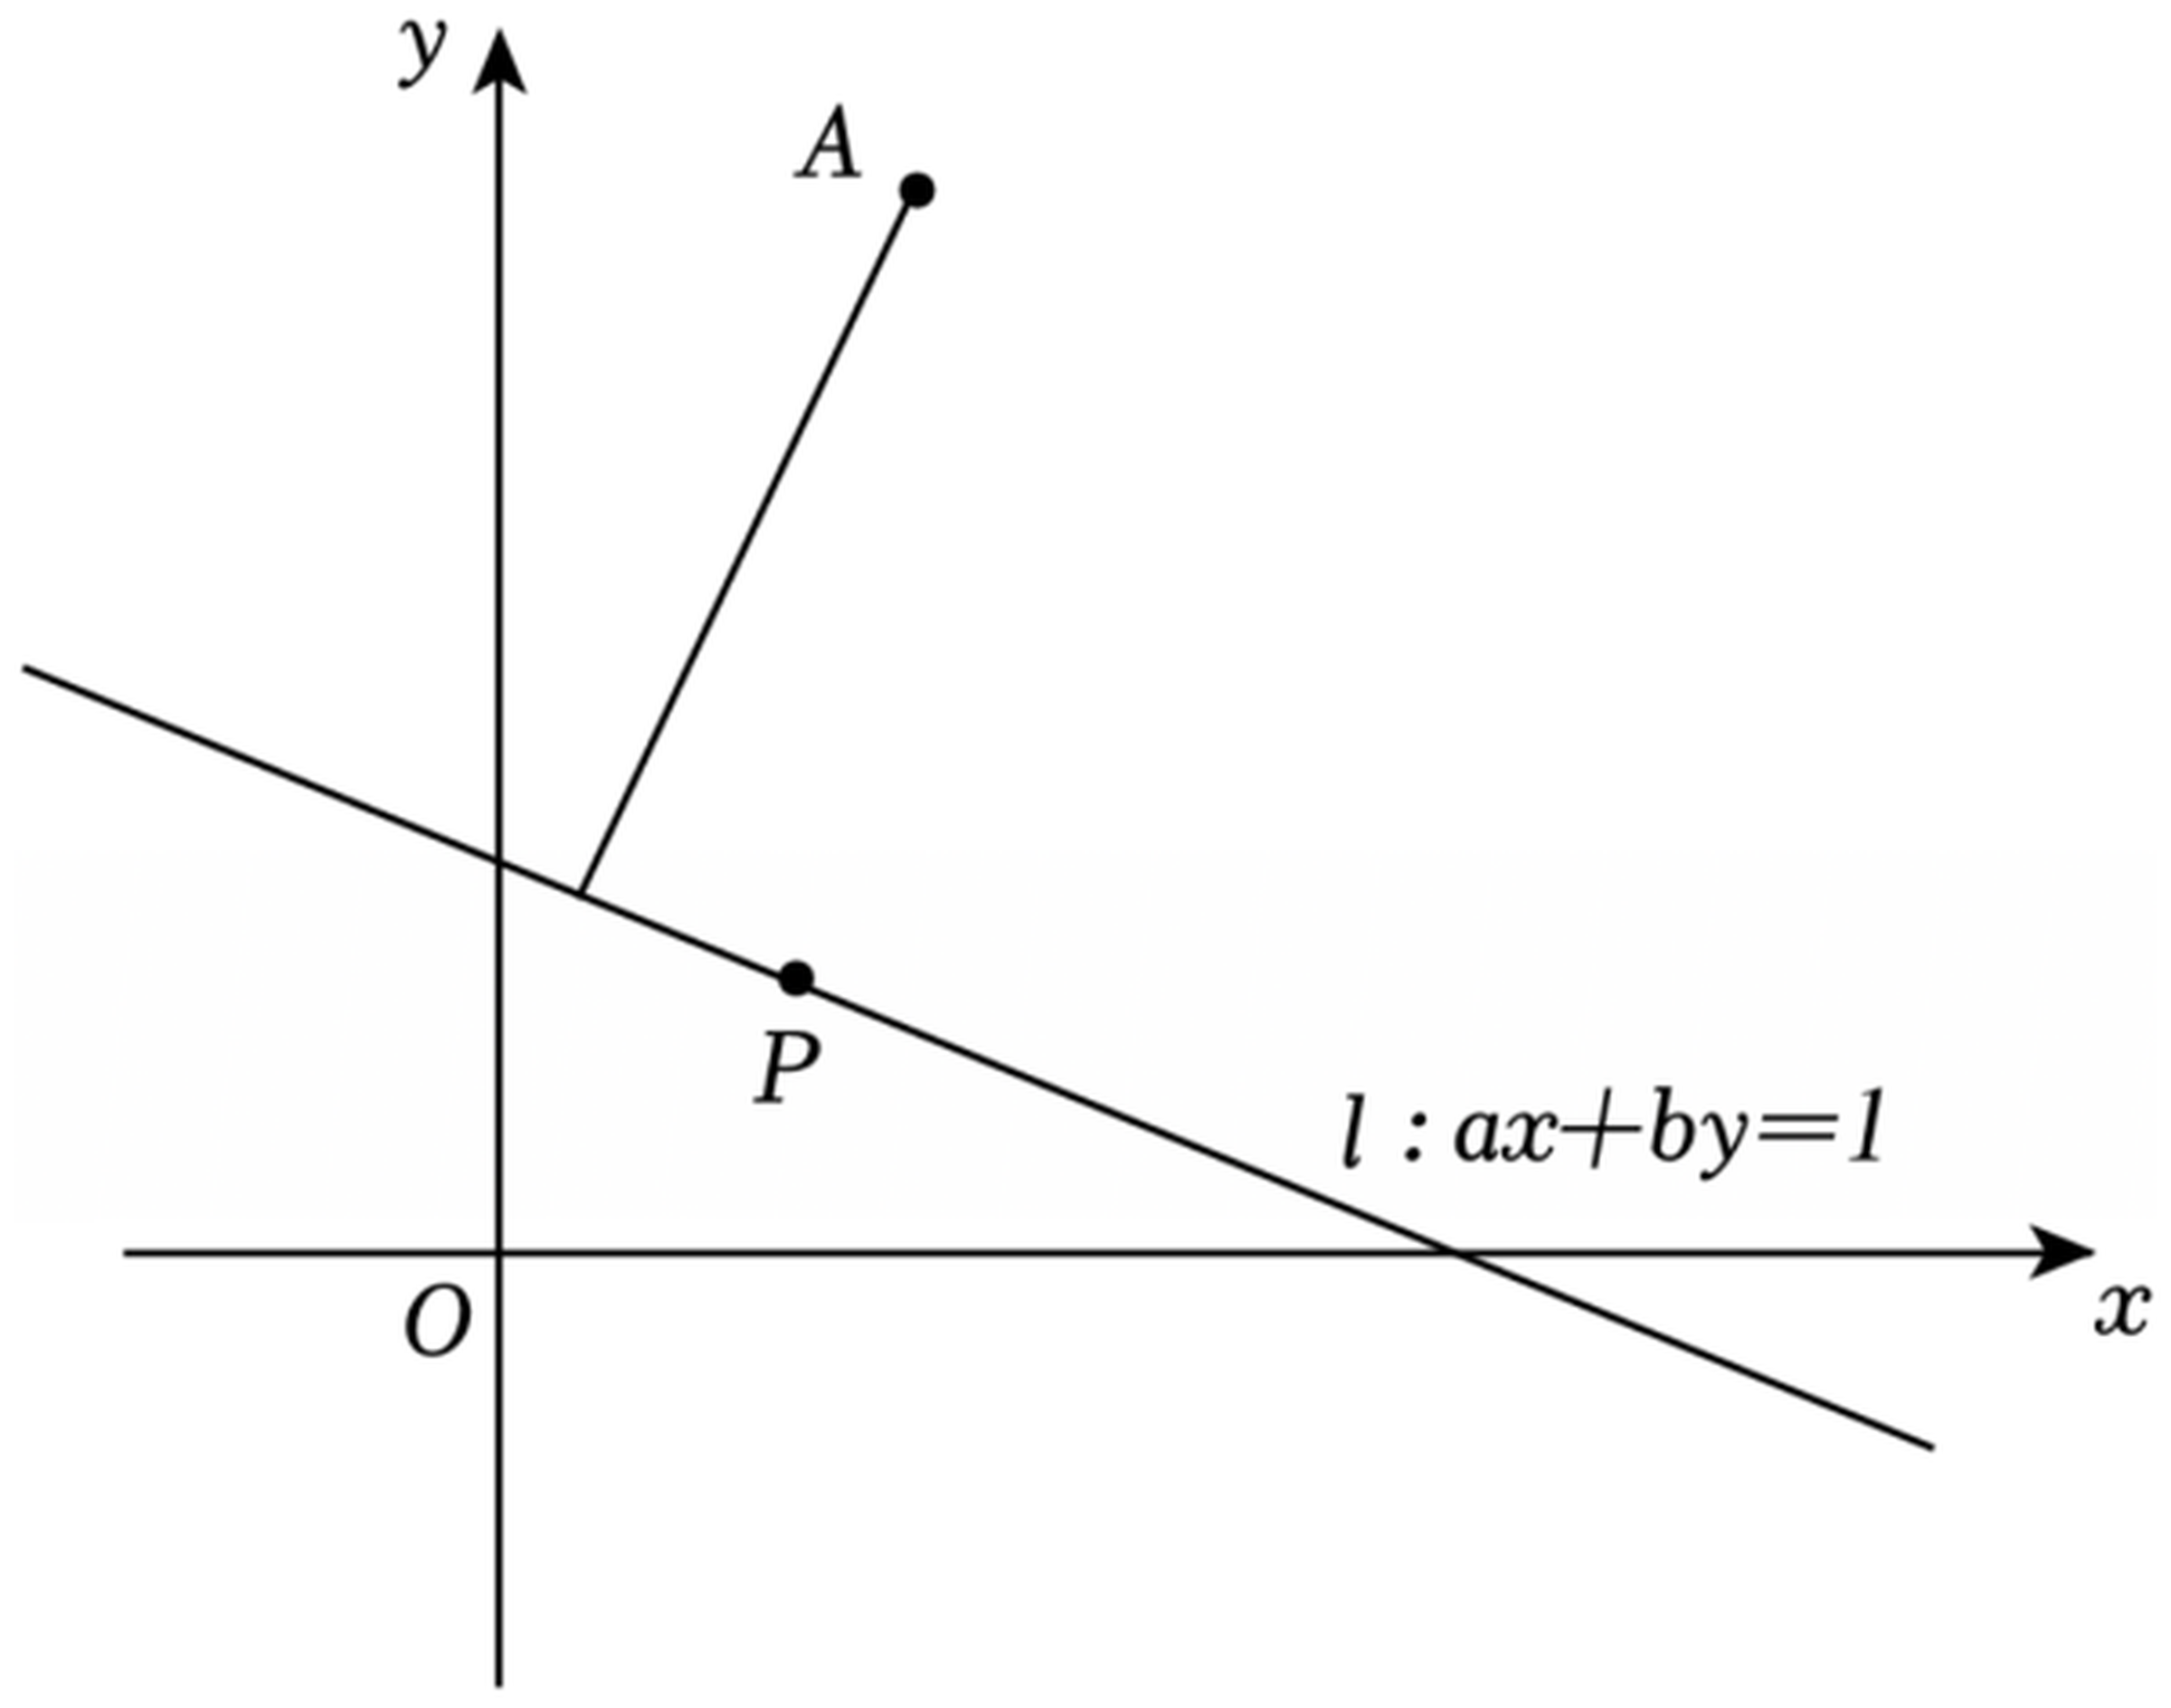
\includegraphics[width=0.56\textwidth]{figures/line_ax_plus_by_1.png}
\end{center}

\step{因为 $a+b=2$，所以直线 $l$ 恒过定点 $P\left(\dfrac12,\dfrac12\right)$，}
\step{再令 $A(1,2)$，则
$d_{A-l}=\dfrac{|a+2b-1|}{\sqrt{a^2+b^2}}\leqslant|AP|=\dfrac{\sqrt{10}}2$，}
\step{当且仅当 $l\perp AP$ 时等号成立，}
\step{又 $\dfrac{a+2b-1}{\sqrt{a^2+b^2}}\leqslant\dfrac{|a+2b-1|}{\sqrt{a^2+b^2}}$，
而当 $l\perp AP$，$a+2b-1>0$，等号也成立，}
\step{故 $\left(\dfrac{a+2b-1}{\sqrt{a^2+b^2}}\right)_{\max}=\dfrac{\sqrt{10}}2$.}
\solend

\fi

\ansspace[6]

\item （1）设 $a$、$b$、$c$ 都是正数，试证明不等式：
$\dfrac{b+c}a+\dfrac{c+a}b+\dfrac{a+b}c\geqslant6$；

（2）对一切正整数 $n$，不等式 $\dfrac{2x-1}x>\dfrac n{n+1}$ 恒成立，
则实数 $x$ 的取值范围构成的集合.

\ifanswer
\solbegin
\stepm{(1)}{因为 $a>0$，$b>0$，$c>0$，}
\step{所以 $\dfrac ba+\dfrac ab\geqslant2$，$\dfrac ca+\dfrac ac\geqslant2$，
$\dfrac cb+\dfrac bc\geqslant2$，}
\step{所以 $\left(\dfrac ba+\dfrac ab\right)+\left(\dfrac ca+\dfrac ac\right)
+\left(\dfrac cb+\dfrac bc\right)\geqslant6$，
即 $\dfrac{b+c}a+\dfrac{c+a}b+\dfrac{a+b}c\geqslant6$.}
% 注：下一行题干原卷作「……则实数 $x$ 的取值范围构成的集合.」，缺一个「求」字，
%     照抄未改，见文件头「原卷存疑」⑤。
\stepm{(2)}{考查 $y=\dfrac n{n+1}=1-\dfrac1{n+1}$，一切正整数 $n$ 函数为严格增函数，
所以 $y\geqslant\dfrac12$，}
\step{对一切正整数 $n$，不等式 $\dfrac{2x-1}x>\dfrac n{n+1}$ 恒成立，
所以 $\dfrac{2x-1}x\geqslant1$，}
\step{所以 $\dfrac{x-1}x\geqslant0$，所以 $x<0$ 或 $x\geqslant1$，}
\step{所以实数 $x$ 的取值范围是 $(-\infty,0)\cup[1,+\infty)$.}
\solend

\fi

\ansspace[6]

\end{enumerate}

\end{document}
"
% 紧凑版：xelatex "\def\iscompact{1}% 高一34_交附闵行_查漏补缺卷.tex
%   —— 高一上数学「2026-2027 年交附闵行高一上查漏补缺卷」（试卷版/答案版）
% 试卷版：xelatex 高一34_交附闵行_查漏补缺卷.tex
% 答案版：xelatex "\def\isanswer{1}\input{高一34_交附闵行_查漏补缺卷.tex}"
% 紧凑版：xelatex "\def\iscompact{1}\input{高一34_交附闵行_查漏补缺卷.tex}"
%
% 原始材料是微信公众号图文（公众号「魔都数学加油站」连载「27学年高一 34」，2026-09-25 发布，
% 原文标题「27学年高一34——2026-2027年上海市交附闵行高一上查漏补缺卷」），
% 正文为 7 张 PNG 页（均 2560×3620），取 mmbiz.qpic.cn/<hash>/0 的原图档。
% 原文本身就是一份**讲评版**，但**全卷没有任何一处印「【答案】」**——每题下方直接印【解析】，
% 答案写在解析的末句。试题文字与解析均照原卷录入，未改内容。
% 卷面的粉色斜水印属水印，未录入。
%
% 卷首标题：原卷印作「2026-2027 年交附闵行高一上查漏补缺卷」（公众号标题里的「上海市」
% 三字卷面标题行没有，本稿照卷面），年份区间按全稿惯例排 en dash，前缀照原卷保留「年」。
%
% 与原卷的排版差异（均已在 README「说明」中交代）：
%   ① 原文自**第 3 题**起（第 1、2 题未在该文中发布），故本稿题号亦自 3 起；
%   ② 原卷只有「一、填空题」「二、解答题」两个节标题（本卷无选择题），本稿照原卷分节，
%      只把标题改排成全稿统一的「大节标题」样式；
%   ③ 原卷通篇只印【解析】（无【答案】行），本稿统一改为试卷版隐去、答案版以 \ifanswer{}
%      块给出，两版彻底分离；
%   ④ 数集记号原卷两套并用：第 4 题与第 11(2) 题作斜体的 $R$，第 7 题两处作粗体的
%      $\mathbf{R}^+$，本稿按全稿惯例统一写作 $\R$；
%   ⑤ 原卷填空的横线约两个字宽，本稿按全稿惯例统一排 \blankline[4.4em]（第 9 题的第一个空
%      原卷**没有**下划线、只留了一个空格，本稿仍补出横线，见文件头「原卷存疑」①）；
%   ⑥ 原卷未印副标题，本稿按全稿惯例补出副标题「集合与常用逻辑用语」（本卷实为基本不等式
%      专题，与 高一27／高一28 同样只标主章节，见文末「高一34 专记」）；
%   ⑦ 第 13 题的配图只出现在【解析】里（题干并未写「如图」），故放进 \ifanswer 块，
%      试卷版不排；图取原卷截图、4× LANCZOS 放大（figures/line_ax_plus_by_1.png）。
%
% 原卷存疑五处（均照抄原卷、未改，见源码中该处上方注释）：
%   ① 第 9 题「则 $ab$ 的最大值为 ，」——第一个空后面只有空格、没有下划线，第二个空才有；
%   ② 第 11(2) 题题干括号内写「$a$、$b\in R$」，但函数式 $f(x)=ax^2+(3a-4)x-12$ 里并没有 $b$；
%   ③ 第 10 题只限定 $a$ 是正实数，未提 $b$ 的取值范围；
%   ④ 第 13 题题干作「求 …… 的最大值为____.」（「求」与「为」混用），且**题干未写「如图」**，
%      是【解析】里才写「如图」；
%   ⑤ 第 14(2) 题题干作「……则实数 $x$ 的取值范围构成的集合.」——缺一个「求」字。
% 另有两处标点照录：第 9 题【解析】首句末是句号、第 11(1)① 解析末句是分号。

\documentclass[a4paper,11pt]{article}
\usepackage{common}

\begin{document}

\examtitlest[3]{2026--2027 年交附闵行高一上查漏补缺卷}{集合与常用逻辑用语}

\bigsec{一、填空题}

\begin{enumerate}
\setcounter{enumi}{2}

\item 已知正实数 $m$、$n$ 满足 $\dfrac1{m+2n}+\dfrac1{2m+n}=1$，则 $m+n$ 的最小值为
\blankline[4.4em].

\ifanswer
\solbegin
\step{因为 $m$、$n\in(0,+\infty)$，$\dfrac1{m+2n}+\dfrac1{2m+n}=1$，}
\step{所以 $m+n=\dfrac13[(m+2n)+(2m+n)]\left(\dfrac1{m+2n}+\dfrac1{2m+n}\right)$}
\step{$=\dfrac13\left[2+\dfrac{2m+n}{m+2n}+\dfrac{m+2n}{2m+n}\right]
\geqslant\dfrac13\left[2+2\sqrt{\dfrac{2m+n}{m+2n}\cdot\dfrac{m+2n}{2m+n}}\right]
=\dfrac43$，}
\step{当且仅当 $\dfrac{2m+n}{m+2n}=\dfrac{m+2n}{2m+n}$，即 $m=n=\dfrac23$ 时取等号，}
\step{所以 $m+n$ 的最小值为 $\dfrac43$.}
\solend

\fi

\item 若 $a$、$b\in\R$，且 $a^2+2ab-3b^2=1$，则 $a^2+b^2$ 的最小值为 \blankline[4.4em].

\ifanswer
\solbegin
\step{由 $a^2+2ab-3b^2=1$ 得 $(a+3b)(a-b)=1$，}
\step{令 $x=a+3b$，$y=a-b$，则 $xy=1$ 且 $a=\dfrac{x+3y}4$，$b=\dfrac{x-y}4$，}
\step{所以 $a^2+b^2=\left(\dfrac{x+3y}4\right)^2+\left(\dfrac{x-y}4\right)^2
=\dfrac{x^2+5y^2+2}8\geqslant\dfrac{2\sqrt{5x^2y^2}+2}8=\dfrac{\sqrt5+1}4$，}
\step{当且仅当 $x^2=\sqrt5$，$y^2=\dfrac{\sqrt5}5$ 时取等号，
故 $a^2+b^2$ 的最小值为 $\dfrac{\sqrt5+1}4$.}
\solend

\fi

\item 已知实数 $x$、$y$ 满足 $3x^2+3y^2-2xy=4$，则 $x+y$ 的最大值为 \blankline[4.4em].

\ifanswer
\solbegin
\step{由 $3x^2+3y^2-2xy=4$，则 $3[(x+y)^2-2xy]-2xy=4$，}
\step{设 $s=x+y$，则 $3s^2-8xy=4$，即 $xy=\dfrac{3s^2-4}8$，}
\step{对任意实数 $x$、$y$，有 $xy\leqslant\left(\dfrac{x+y}2\right)^2=\dfrac{s^2}4$，
即 $\dfrac{3s^2-4}8\leqslant\dfrac{s^2}4$，}
\step{得 $s^2\leqslant4$，即 $-2\leqslant s\leqslant2$，}
\step{当 $x=y=1$ 时，满足原等式，且 $x+y=2$ 成立，因此 $x+y$ 的最大值为 $2$.}
\solend

\fi

\item 若 $a$、$b$、$c$ 都是正实数，则 $\dfrac{a^2+2b^2+4c^2}{ab+2bc}$ 的最小值为
\blankline[4.4em].

\ifanswer
\solbegin
\step{因为 $a^2+2b^2+4c^2=a^2+b^2+b^2+4c^2=(a^2+b^2)+(b^2+4c^2)\geqslant2ab+4bc$，}
\step{所以 $\dfrac{a^2+2b^2+4c^2}{ab+2bc}\geqslant\dfrac{2ab+4bc}{ab+2bc}=2$，
当且仅当 $a=b=2c$ 时取等号，}
\step{即 $\dfrac{a^2+2b^2+4c^2}{ab+2bc}$ 的最小值是 $2$.}
\solend

\fi

\item 已知 $a$、$b\in\R^+$，且 $ab=2$，则 $\dfrac b{2+a^2}+\dfrac a{2+b^2}$ 的最小值是
\blankline[4.4em].

\ifanswer
\solbegin
\step{$\dfrac b{2+a^2}+\dfrac a{2+b^2}=\dfrac b{ab+a^2}+\dfrac a{ab+b^2}
=\dfrac b{a(a+b)}+\dfrac a{b(a+b)}$}
\step{$=\dfrac{(a+b)^2-4}{2(a+b)}=\dfrac{a+b}2-\dfrac2{a+b}$，}
\step{令 $t=a+b$，则原式可设为 $y=\dfrac t2-\dfrac2t$ 的函数，}
\step{当 $t>0$ 时，此函数为严格增函数，}
\step{因为 $a$、$b\in\R^+$ 且 $ab=2$，$t=a+b\geqslant2\sqrt{ab}=2\sqrt2$，}
\step{当且仅当 $a=b=\sqrt2$ 时，$t$ 的最小值为 $2\sqrt2$，}
\step{$y=\dfrac t2-\dfrac2t$ 在 $t\in[2\sqrt2,+\infty)$ 上严格增，}
\step{所以原式的最小值为 $\dfrac{2\sqrt2}2-\dfrac2{2\sqrt2}=\dfrac{\sqrt2}2$，
则 $\dfrac b{2+a^2}+\dfrac a{2+b^2}$ 的最小值是 $\dfrac{\sqrt2}2$.}
\solend

\fi

\item 设 $x$、$y$、$z$ 为正实数，满足 $x-2y+3z=0$，则 $\dfrac{y^2}{xz}$ 的最小值是
\blankline[4.4em].

\ifanswer
\solbegin
\step{因为 $x-2y+3z=0$，所以 $y=\dfrac{x+3z}2$，}
\step{所以 $\dfrac{y^2}{xz}=\dfrac{x^2+9z^2+6xz}{4xz}\geqslant\dfrac{6xz+6xz}{4xz}=3$，
当且仅当 $x=3z$ 时取等号，}
\step{故 $\dfrac{y^2}{xz}$ 的最小值是 $3$.}
\solend

\fi

% 注：下一题的第一个空原卷只留了一个空格、**没有**下划线（第二个空才有），本稿仍按全稿
%     惯例补出横线；另其【解析】首句末原卷作句号，照录。见文件头「原卷存疑」①。
\item 设 $a$、$b$ 为正实数，且 $a+b=3$，则 $ab$ 的最大值为 \blankline[4.4em]，
$\dfrac{a^2}{a+2}+\dfrac{b^2}{b+1}$ 的最小值为 \blankline[4.4em].

\ifanswer
\solbegin
\step{因为 $a>0$，$b>0$，所以 $a+b=3\geqslant2\sqrt{ab}$，}
\step{故 $ab$ 的最大值为 $\dfrac94$，当且仅当 $a=b=\dfrac32$ 时取等号.}
\step{令 $a+2=m$，$b+1=n$，则 $m+n=a+b+3=6$，}
\step{解得 $a=m-2$，$b=n-1$，}
\step{所以 $\dfrac{a^2}{a+2}+\dfrac{b^2}{b+1}=\dfrac{(m-2)^2}m+\dfrac{(n-1)^2}n
=m+\dfrac4m+n+\dfrac1n-6=\dfrac4m+\dfrac1n$}
\step{$=\dfrac16(m+n)\left(\dfrac4m+\dfrac1n\right)
=\dfrac16\left(\dfrac{4n}m+\dfrac mn+5\right)\geqslant\dfrac16(4+5)=\dfrac32$，}
\step{当且仅当 $\dfrac{4n}m=\dfrac mn$ 时，即 $m=2n$ 时
$\dfrac{a^2}{a+2}+\dfrac{b^2}{b+1}$ 取得最小值，}
\step{因此 $\dfrac{a^2}{a+2}+\dfrac{b^2}{b+1}$ 的最小值为 $\dfrac32$.}
\solend

\fi

\item 若 $a$ 是正实数，$2a^2+3b^2=10$，则 $a\sqrt{2+b^2}$ 的最大值是 \blankline[4.4em].

\ifanswer
\solbegin
\step{$a$ 是正实数，$2a^2+3b^2=10$，变形为 $2a^2+3(b^2+2)=16$，}
\step{所以 $16\geqslant2\sqrt{2a^2\times3(b^2+2)}=2\sqrt6\cdot a\sqrt{b^2+2}$，
得 $a\sqrt{2+b^2}\leqslant\dfrac{4\sqrt6}3$，}
\step{当且仅当 $2a^2=3(b^2+2)=8$，即 $a=2$，$b^2=\dfrac23$ 时取等号，}
\step{所以 $a\sqrt{2+b^2}$ 的最大值为 $\dfrac{4\sqrt6}3$.}
\solend

\fi

\end{enumerate}

\bigsec{二、解答题}

\begin{enumerate}
\setcounter{enumi}{10}

\item （1）已知 $x>0$，$y>0$，$2xy=x+4y$. ①求 $xy$ 的最小值；②求 $x+y$ 的最小值.

（2）已知函数 $f(x)=ax^2+(3a-4)x-12$（$a$、$b\in\R$），求不等式 $f(x)\geqslant0$ 的解集.

\ifanswer
\solbegin
\stepm{(1)}{①因为 $x>0$，$y>0$，由基本不等式得
$2xy=x+4y\geqslant2\sqrt{4xy}=4\sqrt{xy}$，}
\step{解得 $xy\geqslant4$，当且仅当 $x=4y=4$ 时取等号，故 $xy$ 的最小值为 $4$；}
\step{②因为 $x>0$，$y>0$，由已知条件得 $\dfrac{4y+x}{xy}=\dfrac4x+\dfrac1y=2$，}
\step{所以 $x+y=\dfrac12(x+y)\left(\dfrac4x+\dfrac1y\right)
=\dfrac12\left(5+\dfrac{4y}x+\dfrac xy\right)
\geqslant\dfrac12\left(5+2\sqrt{\dfrac{4y}x\cdot\dfrac xy}\right)=\dfrac92$，}
\step{当且仅当 $x=2y=3$ 时，等号成立，故 $x+y$ 的最小值为 $\dfrac92$；}
% 注：下一行题干括号内原卷写「$a$、$b\in R$」，但函数式里并没有 $b$，照抄未改，
%     见文件头「原卷存疑」②。
\stepm{(2)}{当 $a=0$ 时，则 $x+3\leqslant0$，解得 $x\leqslant-3$；}
\step{当 $a\neq0$ 时，$f(x)=ax^2+(3a-4)x-12=(x+3)(ax-4)
=a(x+3)\left(x-\dfrac4a\right)$，}
\step{当 $a>0$ 时，则 $(x+3)\left(x-\dfrac4a\right)\geqslant0$，
解得 $x\leqslant-3$ 或 $x\geqslant\dfrac4a$；}
\step{当 $a<0$ 时，则 $(x+3)\left(x-\dfrac4a\right)\leqslant0$，}
\step{当 $\dfrac4a>-3$ 时，即 $a<-\dfrac43$，解 $(x+3)\left(x-\dfrac4a\right)\leqslant0$，
得 $-3\leqslant x\leqslant\dfrac4a$；}
\step{当 $\dfrac4a=-3$ 时，即 $a=-\dfrac43$，解 $(x+3)\left(x-\dfrac4a\right)\leqslant0$，
得 $x=-3$；}
\step{当 $\dfrac4a<-3$ 时，即 $-\dfrac43<a<0$，解 $(x+3)\left(x-\dfrac4a\right)\leqslant0$，
得 $\dfrac4a\leqslant x\leqslant-3$；}
\step{综上所述，当 $a<-\dfrac43$ 时，不等式 $f(x)\geqslant0$ 的解集为
$\left[-3,\dfrac4a\right]$；}
\step{当 $a=-\dfrac43$ 时，不等式 $f(x)\geqslant0$ 的解集为 $\{-3\}$；}
\step{当 $-\dfrac43<a<0$ 时，不等式 $f(x)\geqslant0$ 的解集为
$\left[\dfrac4a,-3\right]$；}
\step{当 $a=0$ 时，不等式 $f(x)\geqslant0$ 的解集为 $(-\infty,-3]$；}
\step{当 $a>0$ 时，不等式 $f(x)\geqslant0$ 的解集为
$(-\infty,-3]\cup\left[\dfrac4a,+\infty\right)$.}
\solend

\fi

\ansspace[8]

\item 已知 $x$、$y$ 都是正数，且 $\dfrac2x+\dfrac1y=1$.

\begin{enumerate}[label=(\arabic*)]
\item 求 $2x+y$ 的最小值及此时 $x$、$y$ 的取值；
\item 不等式 $(2x+y)^2\geqslant m(x+2y)$ 恒成立，求实数 $m$ 的取值范围.
\end{enumerate}

\ifanswer
\solbegin
\stepm{(1)}{$2x+y=(2x+y)\left(\dfrac2x+\dfrac1y\right)
=4+\dfrac{2x}y+\dfrac{2y}x+1\geqslant5+2\sqrt{\dfrac{2x}y\cdot\dfrac{2y}x}=9$，}
\step{当且仅当 $x=y$ 且 $\dfrac2x+\dfrac1y=1$，即 $x=y=3$ 时取等号，}
\step{此时 $2x+y$ 的最小值为 $9$.}
\stepm{(2)}{由 $\dfrac2x+\dfrac1y=1$，得 $x+2y=xy>0$，}
\step{故 $(2x+y)^2\geqslant m(x+2y)\Leftrightarrow m\leqslant\dfrac{(2x+y)^2}{x+2y}
\Leftrightarrow m\leqslant\dfrac{(2x+y)^2}{xy}$，}
\step{又 $\dfrac{(2x+y)^2}{xy}=\dfrac{4x^2+y^2+4xy}{xy}
=\dfrac{4x}y+\dfrac yx+4\geqslant2\sqrt{\dfrac{4x}y\cdot\dfrac yx}+4=8$，}
\step{当且仅当 $\begin{cases}\dfrac{4x}y=\dfrac yx\\[2pt]
\dfrac2x+\dfrac1y=1\end{cases}$ 时取等号，$\dfrac{(2x+y)^2}{xy}$ 取得最小值 $8$，}
\step{故 $m$ 的取值范围为 $\{m\mid m\leqslant8\}$.}
\solend

\fi

\ansspace[6]

% 注：本小题题干作「求 …… 的最大值为____.」（「求」与「为」混用），且**题干未写「如图」**
%     ——是【解析】里才写「如图」，照抄未改，见文件头「原卷存疑」④。
\item 已知实数 $a$、$b$ 满足 $a+b=2$，求 $\dfrac{a+2b-1}{\sqrt{a^2+b^2}}$ 的最大值为
\blankline[4.4em].

\ifanswer
\solbegin
\step{如图，考虑直线 $l:ax+by=1$，}

\begin{center}
% 图取原卷截图、4× LANCZOS 放大。图只在【解析】里出现（题干并未写「如图」），
% 故放进 \ifanswer 块，试卷版不排，见文件头⑦。
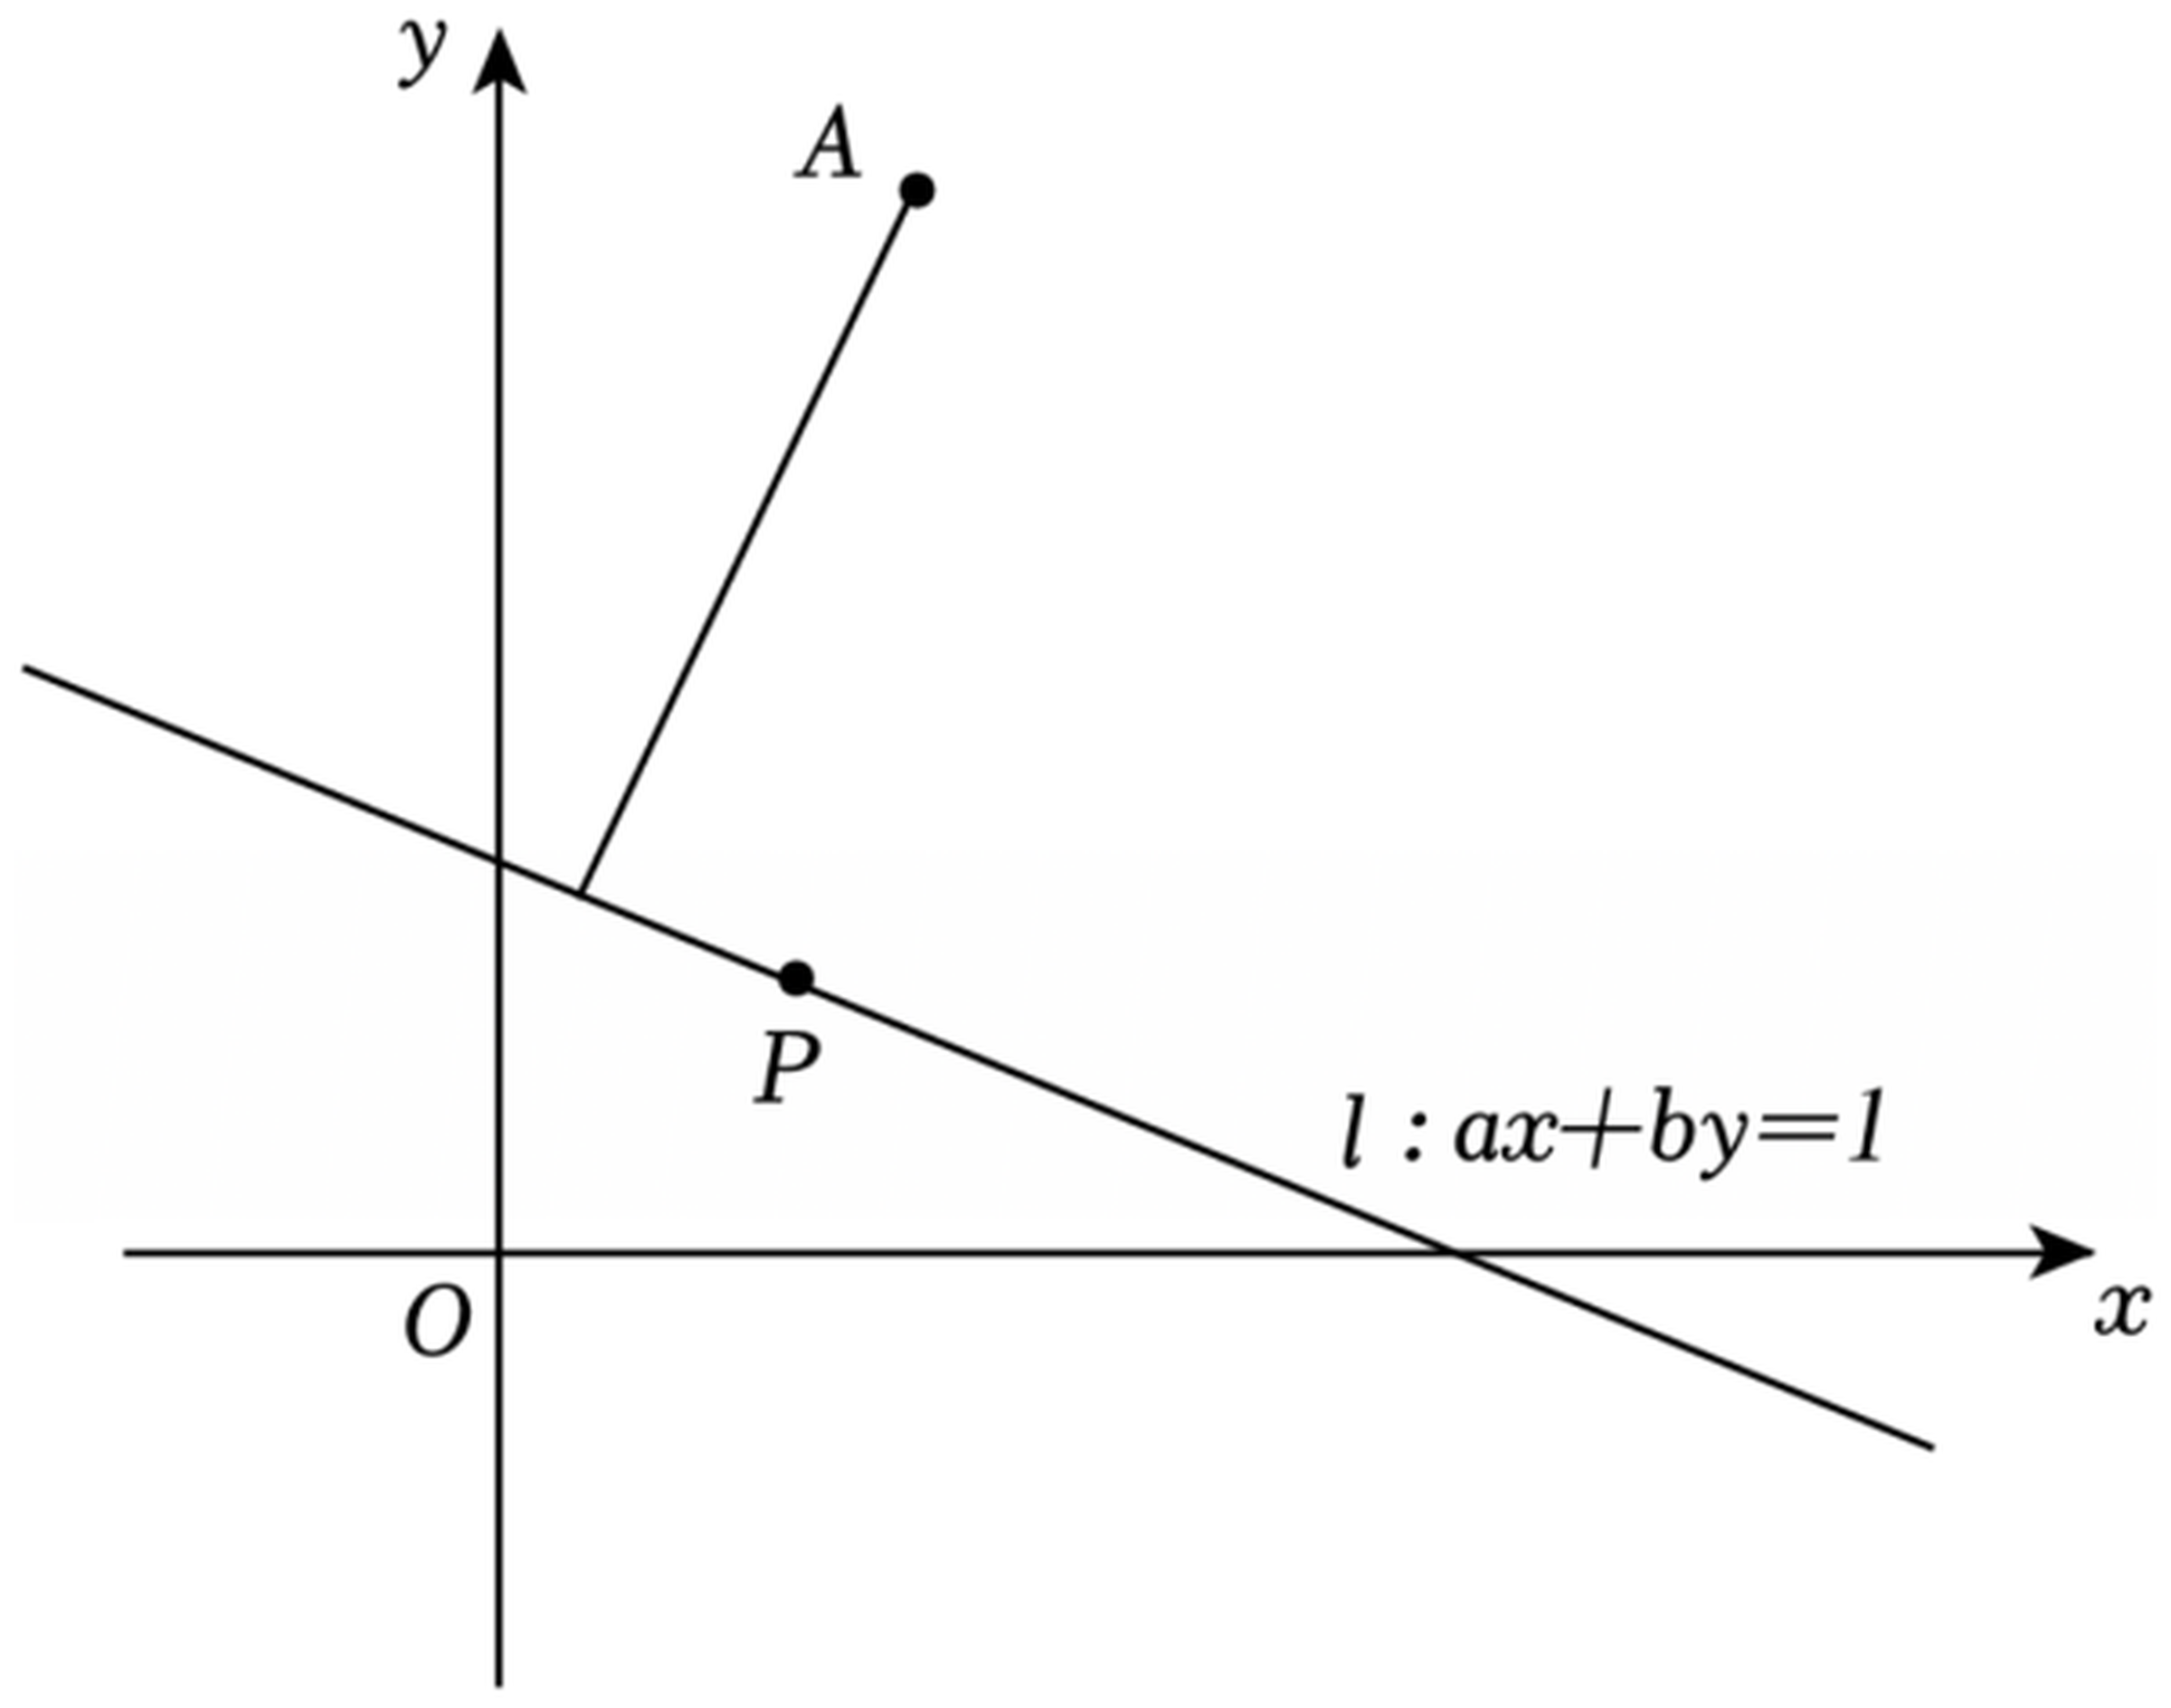
\includegraphics[width=0.56\textwidth]{figures/line_ax_plus_by_1.png}
\end{center}

\step{因为 $a+b=2$，所以直线 $l$ 恒过定点 $P\left(\dfrac12,\dfrac12\right)$，}
\step{再令 $A(1,2)$，则
$d_{A-l}=\dfrac{|a+2b-1|}{\sqrt{a^2+b^2}}\leqslant|AP|=\dfrac{\sqrt{10}}2$，}
\step{当且仅当 $l\perp AP$ 时等号成立，}
\step{又 $\dfrac{a+2b-1}{\sqrt{a^2+b^2}}\leqslant\dfrac{|a+2b-1|}{\sqrt{a^2+b^2}}$，
而当 $l\perp AP$，$a+2b-1>0$，等号也成立，}
\step{故 $\left(\dfrac{a+2b-1}{\sqrt{a^2+b^2}}\right)_{\max}=\dfrac{\sqrt{10}}2$.}
\solend

\fi

\ansspace[6]

\item （1）设 $a$、$b$、$c$ 都是正数，试证明不等式：
$\dfrac{b+c}a+\dfrac{c+a}b+\dfrac{a+b}c\geqslant6$；

（2）对一切正整数 $n$，不等式 $\dfrac{2x-1}x>\dfrac n{n+1}$ 恒成立，
则实数 $x$ 的取值范围构成的集合.

\ifanswer
\solbegin
\stepm{(1)}{因为 $a>0$，$b>0$，$c>0$，}
\step{所以 $\dfrac ba+\dfrac ab\geqslant2$，$\dfrac ca+\dfrac ac\geqslant2$，
$\dfrac cb+\dfrac bc\geqslant2$，}
\step{所以 $\left(\dfrac ba+\dfrac ab\right)+\left(\dfrac ca+\dfrac ac\right)
+\left(\dfrac cb+\dfrac bc\right)\geqslant6$，
即 $\dfrac{b+c}a+\dfrac{c+a}b+\dfrac{a+b}c\geqslant6$.}
% 注：下一行题干原卷作「……则实数 $x$ 的取值范围构成的集合.」，缺一个「求」字，
%     照抄未改，见文件头「原卷存疑」⑤。
\stepm{(2)}{考查 $y=\dfrac n{n+1}=1-\dfrac1{n+1}$，一切正整数 $n$ 函数为严格增函数，
所以 $y\geqslant\dfrac12$，}
\step{对一切正整数 $n$，不等式 $\dfrac{2x-1}x>\dfrac n{n+1}$ 恒成立，
所以 $\dfrac{2x-1}x\geqslant1$，}
\step{所以 $\dfrac{x-1}x\geqslant0$，所以 $x<0$ 或 $x\geqslant1$，}
\step{所以实数 $x$ 的取值范围是 $(-\infty,0)\cup[1,+\infty)$.}
\solend

\fi

\ansspace[6]

\end{enumerate}

\end{document}
"
%
% 原始材料是微信公众号图文（公众号「魔都数学加油站」连载「27学年高一 34」，2026-09-25 发布，
% 原文标题「27学年高一34——2026-2027年上海市交附闵行高一上查漏补缺卷」），
% 正文为 7 张 PNG 页（均 2560×3620），取 mmbiz.qpic.cn/<hash>/0 的原图档。
% 原文本身就是一份**讲评版**，但**全卷没有任何一处印「【答案】」**——每题下方直接印【解析】，
% 答案写在解析的末句。试题文字与解析均照原卷录入，未改内容。
% 卷面的粉色斜水印属水印，未录入。
%
% 卷首标题：原卷印作「2026-2027 年交附闵行高一上查漏补缺卷」（公众号标题里的「上海市」
% 三字卷面标题行没有，本稿照卷面），年份区间按全稿惯例排 en dash，前缀照原卷保留「年」。
%
% 与原卷的排版差异（均已在 README「说明」中交代）：
%   ① 原文自**第 3 题**起（第 1、2 题未在该文中发布），故本稿题号亦自 3 起；
%   ② 原卷只有「一、填空题」「二、解答题」两个节标题（本卷无选择题），本稿照原卷分节，
%      只把标题改排成全稿统一的「大节标题」样式；
%   ③ 原卷通篇只印【解析】（无【答案】行），本稿统一改为试卷版隐去、答案版以 \ifanswer{}
%      块给出，两版彻底分离；
%   ④ 数集记号原卷两套并用：第 4 题与第 11(2) 题作斜体的 $R$，第 7 题两处作粗体的
%      $\mathbf{R}^+$，本稿按全稿惯例统一写作 $\R$；
%   ⑤ 原卷填空的横线约两个字宽，本稿按全稿惯例统一排 \blankline[4.4em]（第 9 题的第一个空
%      原卷**没有**下划线、只留了一个空格，本稿仍补出横线，见文件头「原卷存疑」①）；
%   ⑥ 原卷未印副标题，本稿按全稿惯例补出副标题「集合与常用逻辑用语」（本卷实为基本不等式
%      专题，与 高一27／高一28 同样只标主章节，见文末「高一34 专记」）；
%   ⑦ 第 13 题的配图只出现在【解析】里（题干并未写「如图」），故放进 \ifanswer 块，
%      试卷版不排；图取原卷截图、4× LANCZOS 放大（figures/line_ax_plus_by_1.png）。
%
% 原卷存疑五处（均照抄原卷、未改，见源码中该处上方注释）：
%   ① 第 9 题「则 $ab$ 的最大值为 ，」——第一个空后面只有空格、没有下划线，第二个空才有；
%   ② 第 11(2) 题题干括号内写「$a$、$b\in R$」，但函数式 $f(x)=ax^2+(3a-4)x-12$ 里并没有 $b$；
%   ③ 第 10 题只限定 $a$ 是正实数，未提 $b$ 的取值范围；
%   ④ 第 13 题题干作「求 …… 的最大值为____.」（「求」与「为」混用），且**题干未写「如图」**，
%      是【解析】里才写「如图」；
%   ⑤ 第 14(2) 题题干作「……则实数 $x$ 的取值范围构成的集合.」——缺一个「求」字。
% 另有两处标点照录：第 9 题【解析】首句末是句号、第 11(1)① 解析末句是分号。

\documentclass[a4paper,11pt]{article}
\usepackage{common}

\begin{document}

\examtitlest[3]{2026--2027 年交附闵行高一上查漏补缺卷}{集合与常用逻辑用语}

\bigsec{一、填空题}

\begin{enumerate}
\setcounter{enumi}{2}

\item 已知正实数 $m$、$n$ 满足 $\dfrac1{m+2n}+\dfrac1{2m+n}=1$，则 $m+n$ 的最小值为
\blankline[4.4em].

\ifanswer
\solbegin
\step{因为 $m$、$n\in(0,+\infty)$，$\dfrac1{m+2n}+\dfrac1{2m+n}=1$，}
\step{所以 $m+n=\dfrac13[(m+2n)+(2m+n)]\left(\dfrac1{m+2n}+\dfrac1{2m+n}\right)$}
\step{$=\dfrac13\left[2+\dfrac{2m+n}{m+2n}+\dfrac{m+2n}{2m+n}\right]
\geqslant\dfrac13\left[2+2\sqrt{\dfrac{2m+n}{m+2n}\cdot\dfrac{m+2n}{2m+n}}\right]
=\dfrac43$，}
\step{当且仅当 $\dfrac{2m+n}{m+2n}=\dfrac{m+2n}{2m+n}$，即 $m=n=\dfrac23$ 时取等号，}
\step{所以 $m+n$ 的最小值为 $\dfrac43$.}
\solend

\fi

\item 若 $a$、$b\in\R$，且 $a^2+2ab-3b^2=1$，则 $a^2+b^2$ 的最小值为 \blankline[4.4em].

\ifanswer
\solbegin
\step{由 $a^2+2ab-3b^2=1$ 得 $(a+3b)(a-b)=1$，}
\step{令 $x=a+3b$，$y=a-b$，则 $xy=1$ 且 $a=\dfrac{x+3y}4$，$b=\dfrac{x-y}4$，}
\step{所以 $a^2+b^2=\left(\dfrac{x+3y}4\right)^2+\left(\dfrac{x-y}4\right)^2
=\dfrac{x^2+5y^2+2}8\geqslant\dfrac{2\sqrt{5x^2y^2}+2}8=\dfrac{\sqrt5+1}4$，}
\step{当且仅当 $x^2=\sqrt5$，$y^2=\dfrac{\sqrt5}5$ 时取等号，
故 $a^2+b^2$ 的最小值为 $\dfrac{\sqrt5+1}4$.}
\solend

\fi

\item 已知实数 $x$、$y$ 满足 $3x^2+3y^2-2xy=4$，则 $x+y$ 的最大值为 \blankline[4.4em].

\ifanswer
\solbegin
\step{由 $3x^2+3y^2-2xy=4$，则 $3[(x+y)^2-2xy]-2xy=4$，}
\step{设 $s=x+y$，则 $3s^2-8xy=4$，即 $xy=\dfrac{3s^2-4}8$，}
\step{对任意实数 $x$、$y$，有 $xy\leqslant\left(\dfrac{x+y}2\right)^2=\dfrac{s^2}4$，
即 $\dfrac{3s^2-4}8\leqslant\dfrac{s^2}4$，}
\step{得 $s^2\leqslant4$，即 $-2\leqslant s\leqslant2$，}
\step{当 $x=y=1$ 时，满足原等式，且 $x+y=2$ 成立，因此 $x+y$ 的最大值为 $2$.}
\solend

\fi

\item 若 $a$、$b$、$c$ 都是正实数，则 $\dfrac{a^2+2b^2+4c^2}{ab+2bc}$ 的最小值为
\blankline[4.4em].

\ifanswer
\solbegin
\step{因为 $a^2+2b^2+4c^2=a^2+b^2+b^2+4c^2=(a^2+b^2)+(b^2+4c^2)\geqslant2ab+4bc$，}
\step{所以 $\dfrac{a^2+2b^2+4c^2}{ab+2bc}\geqslant\dfrac{2ab+4bc}{ab+2bc}=2$，
当且仅当 $a=b=2c$ 时取等号，}
\step{即 $\dfrac{a^2+2b^2+4c^2}{ab+2bc}$ 的最小值是 $2$.}
\solend

\fi

\item 已知 $a$、$b\in\R^+$，且 $ab=2$，则 $\dfrac b{2+a^2}+\dfrac a{2+b^2}$ 的最小值是
\blankline[4.4em].

\ifanswer
\solbegin
\step{$\dfrac b{2+a^2}+\dfrac a{2+b^2}=\dfrac b{ab+a^2}+\dfrac a{ab+b^2}
=\dfrac b{a(a+b)}+\dfrac a{b(a+b)}$}
\step{$=\dfrac{(a+b)^2-4}{2(a+b)}=\dfrac{a+b}2-\dfrac2{a+b}$，}
\step{令 $t=a+b$，则原式可设为 $y=\dfrac t2-\dfrac2t$ 的函数，}
\step{当 $t>0$ 时，此函数为严格增函数，}
\step{因为 $a$、$b\in\R^+$ 且 $ab=2$，$t=a+b\geqslant2\sqrt{ab}=2\sqrt2$，}
\step{当且仅当 $a=b=\sqrt2$ 时，$t$ 的最小值为 $2\sqrt2$，}
\step{$y=\dfrac t2-\dfrac2t$ 在 $t\in[2\sqrt2,+\infty)$ 上严格增，}
\step{所以原式的最小值为 $\dfrac{2\sqrt2}2-\dfrac2{2\sqrt2}=\dfrac{\sqrt2}2$，
则 $\dfrac b{2+a^2}+\dfrac a{2+b^2}$ 的最小值是 $\dfrac{\sqrt2}2$.}
\solend

\fi

\item 设 $x$、$y$、$z$ 为正实数，满足 $x-2y+3z=0$，则 $\dfrac{y^2}{xz}$ 的最小值是
\blankline[4.4em].

\ifanswer
\solbegin
\step{因为 $x-2y+3z=0$，所以 $y=\dfrac{x+3z}2$，}
\step{所以 $\dfrac{y^2}{xz}=\dfrac{x^2+9z^2+6xz}{4xz}\geqslant\dfrac{6xz+6xz}{4xz}=3$，
当且仅当 $x=3z$ 时取等号，}
\step{故 $\dfrac{y^2}{xz}$ 的最小值是 $3$.}
\solend

\fi

% 注：下一题的第一个空原卷只留了一个空格、**没有**下划线（第二个空才有），本稿仍按全稿
%     惯例补出横线；另其【解析】首句末原卷作句号，照录。见文件头「原卷存疑」①。
\item 设 $a$、$b$ 为正实数，且 $a+b=3$，则 $ab$ 的最大值为 \blankline[4.4em]，
$\dfrac{a^2}{a+2}+\dfrac{b^2}{b+1}$ 的最小值为 \blankline[4.4em].

\ifanswer
\solbegin
\step{因为 $a>0$，$b>0$，所以 $a+b=3\geqslant2\sqrt{ab}$，}
\step{故 $ab$ 的最大值为 $\dfrac94$，当且仅当 $a=b=\dfrac32$ 时取等号.}
\step{令 $a+2=m$，$b+1=n$，则 $m+n=a+b+3=6$，}
\step{解得 $a=m-2$，$b=n-1$，}
\step{所以 $\dfrac{a^2}{a+2}+\dfrac{b^2}{b+1}=\dfrac{(m-2)^2}m+\dfrac{(n-1)^2}n
=m+\dfrac4m+n+\dfrac1n-6=\dfrac4m+\dfrac1n$}
\step{$=\dfrac16(m+n)\left(\dfrac4m+\dfrac1n\right)
=\dfrac16\left(\dfrac{4n}m+\dfrac mn+5\right)\geqslant\dfrac16(4+5)=\dfrac32$，}
\step{当且仅当 $\dfrac{4n}m=\dfrac mn$ 时，即 $m=2n$ 时
$\dfrac{a^2}{a+2}+\dfrac{b^2}{b+1}$ 取得最小值，}
\step{因此 $\dfrac{a^2}{a+2}+\dfrac{b^2}{b+1}$ 的最小值为 $\dfrac32$.}
\solend

\fi

\item 若 $a$ 是正实数，$2a^2+3b^2=10$，则 $a\sqrt{2+b^2}$ 的最大值是 \blankline[4.4em].

\ifanswer
\solbegin
\step{$a$ 是正实数，$2a^2+3b^2=10$，变形为 $2a^2+3(b^2+2)=16$，}
\step{所以 $16\geqslant2\sqrt{2a^2\times3(b^2+2)}=2\sqrt6\cdot a\sqrt{b^2+2}$，
得 $a\sqrt{2+b^2}\leqslant\dfrac{4\sqrt6}3$，}
\step{当且仅当 $2a^2=3(b^2+2)=8$，即 $a=2$，$b^2=\dfrac23$ 时取等号，}
\step{所以 $a\sqrt{2+b^2}$ 的最大值为 $\dfrac{4\sqrt6}3$.}
\solend

\fi

\end{enumerate}

\bigsec{二、解答题}

\begin{enumerate}
\setcounter{enumi}{10}

\item （1）已知 $x>0$，$y>0$，$2xy=x+4y$. ①求 $xy$ 的最小值；②求 $x+y$ 的最小值.

（2）已知函数 $f(x)=ax^2+(3a-4)x-12$（$a$、$b\in\R$），求不等式 $f(x)\geqslant0$ 的解集.

\ifanswer
\solbegin
\stepm{(1)}{①因为 $x>0$，$y>0$，由基本不等式得
$2xy=x+4y\geqslant2\sqrt{4xy}=4\sqrt{xy}$，}
\step{解得 $xy\geqslant4$，当且仅当 $x=4y=4$ 时取等号，故 $xy$ 的最小值为 $4$；}
\step{②因为 $x>0$，$y>0$，由已知条件得 $\dfrac{4y+x}{xy}=\dfrac4x+\dfrac1y=2$，}
\step{所以 $x+y=\dfrac12(x+y)\left(\dfrac4x+\dfrac1y\right)
=\dfrac12\left(5+\dfrac{4y}x+\dfrac xy\right)
\geqslant\dfrac12\left(5+2\sqrt{\dfrac{4y}x\cdot\dfrac xy}\right)=\dfrac92$，}
\step{当且仅当 $x=2y=3$ 时，等号成立，故 $x+y$ 的最小值为 $\dfrac92$；}
% 注：下一行题干括号内原卷写「$a$、$b\in R$」，但函数式里并没有 $b$，照抄未改，
%     见文件头「原卷存疑」②。
\stepm{(2)}{当 $a=0$ 时，则 $x+3\leqslant0$，解得 $x\leqslant-3$；}
\step{当 $a\neq0$ 时，$f(x)=ax^2+(3a-4)x-12=(x+3)(ax-4)
=a(x+3)\left(x-\dfrac4a\right)$，}
\step{当 $a>0$ 时，则 $(x+3)\left(x-\dfrac4a\right)\geqslant0$，
解得 $x\leqslant-3$ 或 $x\geqslant\dfrac4a$；}
\step{当 $a<0$ 时，则 $(x+3)\left(x-\dfrac4a\right)\leqslant0$，}
\step{当 $\dfrac4a>-3$ 时，即 $a<-\dfrac43$，解 $(x+3)\left(x-\dfrac4a\right)\leqslant0$，
得 $-3\leqslant x\leqslant\dfrac4a$；}
\step{当 $\dfrac4a=-3$ 时，即 $a=-\dfrac43$，解 $(x+3)\left(x-\dfrac4a\right)\leqslant0$，
得 $x=-3$；}
\step{当 $\dfrac4a<-3$ 时，即 $-\dfrac43<a<0$，解 $(x+3)\left(x-\dfrac4a\right)\leqslant0$，
得 $\dfrac4a\leqslant x\leqslant-3$；}
\step{综上所述，当 $a<-\dfrac43$ 时，不等式 $f(x)\geqslant0$ 的解集为
$\left[-3,\dfrac4a\right]$；}
\step{当 $a=-\dfrac43$ 时，不等式 $f(x)\geqslant0$ 的解集为 $\{-3\}$；}
\step{当 $-\dfrac43<a<0$ 时，不等式 $f(x)\geqslant0$ 的解集为
$\left[\dfrac4a,-3\right]$；}
\step{当 $a=0$ 时，不等式 $f(x)\geqslant0$ 的解集为 $(-\infty,-3]$；}
\step{当 $a>0$ 时，不等式 $f(x)\geqslant0$ 的解集为
$(-\infty,-3]\cup\left[\dfrac4a,+\infty\right)$.}
\solend

\fi

\ansspace[8]

\item 已知 $x$、$y$ 都是正数，且 $\dfrac2x+\dfrac1y=1$.

\begin{enumerate}[label=(\arabic*)]
\item 求 $2x+y$ 的最小值及此时 $x$、$y$ 的取值；
\item 不等式 $(2x+y)^2\geqslant m(x+2y)$ 恒成立，求实数 $m$ 的取值范围.
\end{enumerate}

\ifanswer
\solbegin
\stepm{(1)}{$2x+y=(2x+y)\left(\dfrac2x+\dfrac1y\right)
=4+\dfrac{2x}y+\dfrac{2y}x+1\geqslant5+2\sqrt{\dfrac{2x}y\cdot\dfrac{2y}x}=9$，}
\step{当且仅当 $x=y$ 且 $\dfrac2x+\dfrac1y=1$，即 $x=y=3$ 时取等号，}
\step{此时 $2x+y$ 的最小值为 $9$.}
\stepm{(2)}{由 $\dfrac2x+\dfrac1y=1$，得 $x+2y=xy>0$，}
\step{故 $(2x+y)^2\geqslant m(x+2y)\Leftrightarrow m\leqslant\dfrac{(2x+y)^2}{x+2y}
\Leftrightarrow m\leqslant\dfrac{(2x+y)^2}{xy}$，}
\step{又 $\dfrac{(2x+y)^2}{xy}=\dfrac{4x^2+y^2+4xy}{xy}
=\dfrac{4x}y+\dfrac yx+4\geqslant2\sqrt{\dfrac{4x}y\cdot\dfrac yx}+4=8$，}
\step{当且仅当 $\begin{cases}\dfrac{4x}y=\dfrac yx\\[2pt]
\dfrac2x+\dfrac1y=1\end{cases}$ 时取等号，$\dfrac{(2x+y)^2}{xy}$ 取得最小值 $8$，}
\step{故 $m$ 的取值范围为 $\{m\mid m\leqslant8\}$.}
\solend

\fi

\ansspace[6]

% 注：本小题题干作「求 …… 的最大值为____.」（「求」与「为」混用），且**题干未写「如图」**
%     ——是【解析】里才写「如图」，照抄未改，见文件头「原卷存疑」④。
\item 已知实数 $a$、$b$ 满足 $a+b=2$，求 $\dfrac{a+2b-1}{\sqrt{a^2+b^2}}$ 的最大值为
\blankline[4.4em].

\ifanswer
\solbegin
\step{如图，考虑直线 $l:ax+by=1$，}

\begin{center}
% 图取原卷截图、4× LANCZOS 放大。图只在【解析】里出现（题干并未写「如图」），
% 故放进 \ifanswer 块，试卷版不排，见文件头⑦。
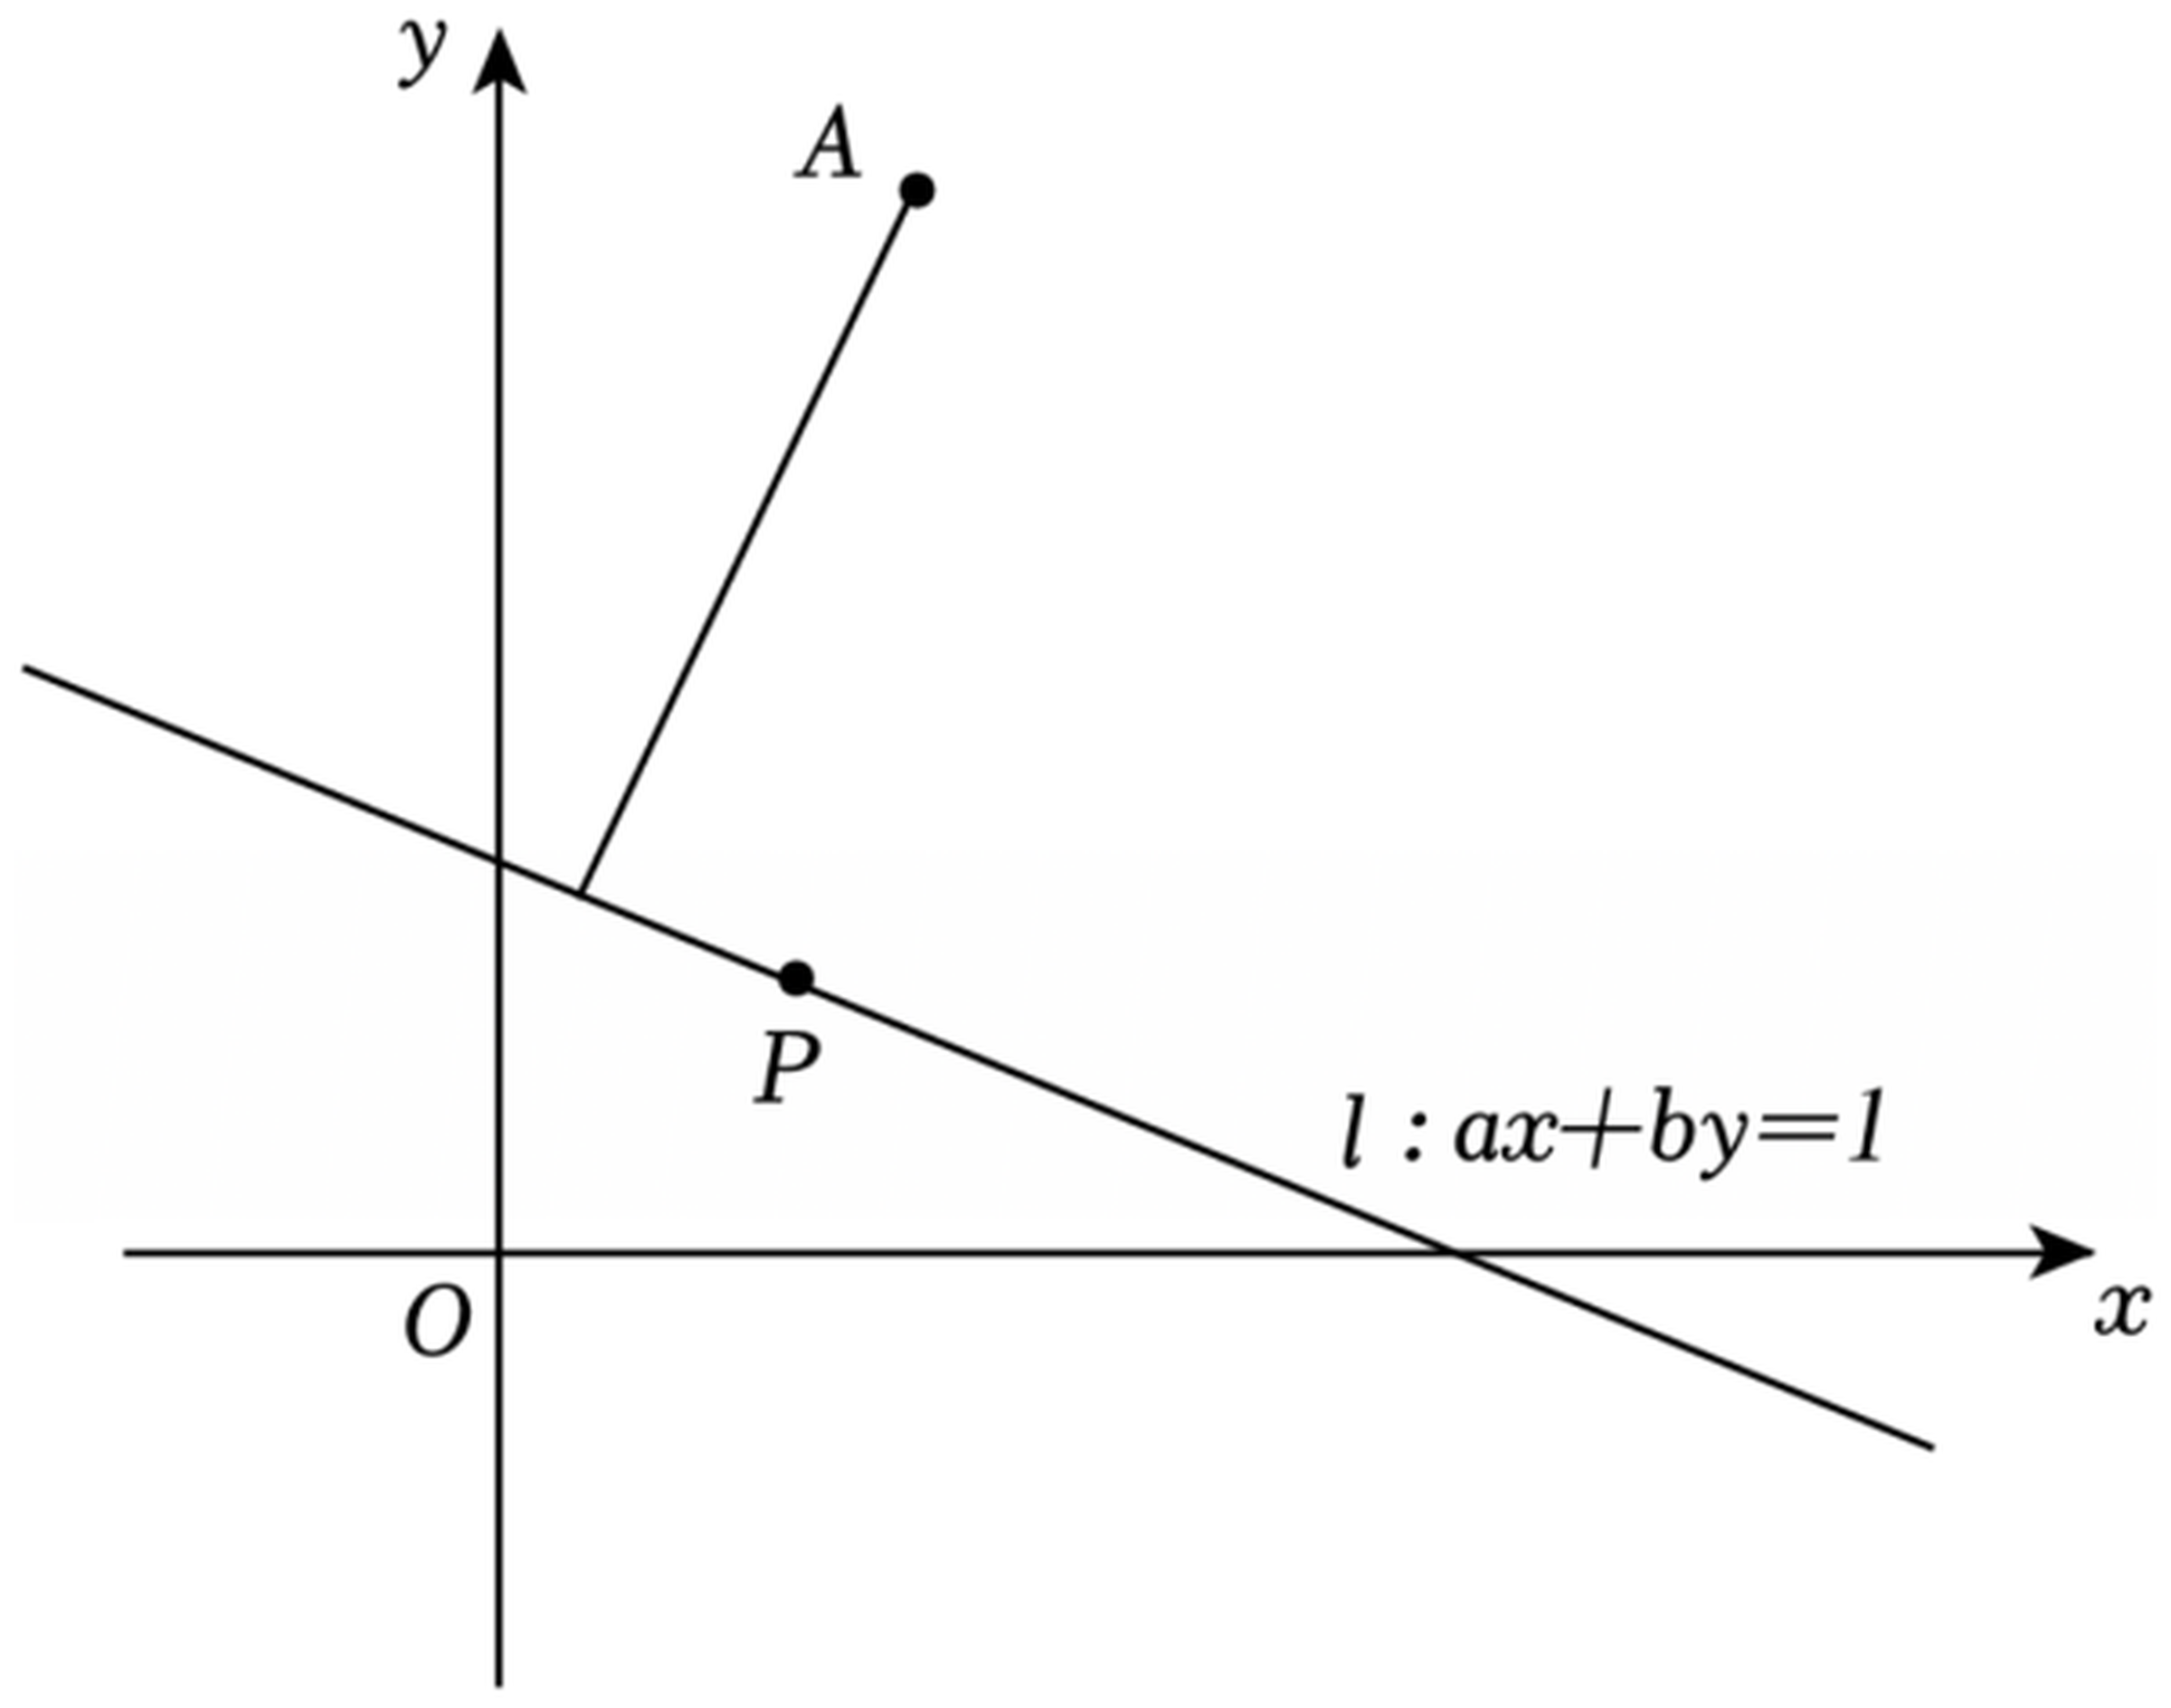
\includegraphics[width=0.56\textwidth]{figures/line_ax_plus_by_1.png}
\end{center}

\step{因为 $a+b=2$，所以直线 $l$ 恒过定点 $P\left(\dfrac12,\dfrac12\right)$，}
\step{再令 $A(1,2)$，则
$d_{A-l}=\dfrac{|a+2b-1|}{\sqrt{a^2+b^2}}\leqslant|AP|=\dfrac{\sqrt{10}}2$，}
\step{当且仅当 $l\perp AP$ 时等号成立，}
\step{又 $\dfrac{a+2b-1}{\sqrt{a^2+b^2}}\leqslant\dfrac{|a+2b-1|}{\sqrt{a^2+b^2}}$，
而当 $l\perp AP$，$a+2b-1>0$，等号也成立，}
\step{故 $\left(\dfrac{a+2b-1}{\sqrt{a^2+b^2}}\right)_{\max}=\dfrac{\sqrt{10}}2$.}
\solend

\fi

\ansspace[6]

\item （1）设 $a$、$b$、$c$ 都是正数，试证明不等式：
$\dfrac{b+c}a+\dfrac{c+a}b+\dfrac{a+b}c\geqslant6$；

（2）对一切正整数 $n$，不等式 $\dfrac{2x-1}x>\dfrac n{n+1}$ 恒成立，
则实数 $x$ 的取值范围构成的集合.

\ifanswer
\solbegin
\stepm{(1)}{因为 $a>0$，$b>0$，$c>0$，}
\step{所以 $\dfrac ba+\dfrac ab\geqslant2$，$\dfrac ca+\dfrac ac\geqslant2$，
$\dfrac cb+\dfrac bc\geqslant2$，}
\step{所以 $\left(\dfrac ba+\dfrac ab\right)+\left(\dfrac ca+\dfrac ac\right)
+\left(\dfrac cb+\dfrac bc\right)\geqslant6$，
即 $\dfrac{b+c}a+\dfrac{c+a}b+\dfrac{a+b}c\geqslant6$.}
% 注：下一行题干原卷作「……则实数 $x$ 的取值范围构成的集合.」，缺一个「求」字，
%     照抄未改，见文件头「原卷存疑」⑤。
\stepm{(2)}{考查 $y=\dfrac n{n+1}=1-\dfrac1{n+1}$，一切正整数 $n$ 函数为严格增函数，
所以 $y\geqslant\dfrac12$，}
\step{对一切正整数 $n$，不等式 $\dfrac{2x-1}x>\dfrac n{n+1}$ 恒成立，
所以 $\dfrac{2x-1}x\geqslant1$，}
\step{所以 $\dfrac{x-1}x\geqslant0$，所以 $x<0$ 或 $x\geqslant1$，}
\step{所以实数 $x$ 的取值范围是 $(-\infty,0)\cup[1,+\infty)$.}
\solend

\fi

\ansspace[6]

\end{enumerate}

\end{document}
"
% 紧凑版：xelatex "\def\iscompact{1}% 高一34_交附闵行_查漏补缺卷.tex
%   —— 高一上数学「2026-2027 年交附闵行高一上查漏补缺卷」（试卷版/答案版）
% 试卷版：xelatex 高一34_交附闵行_查漏补缺卷.tex
% 答案版：xelatex "\def\isanswer{1}% 高一34_交附闵行_查漏补缺卷.tex
%   —— 高一上数学「2026-2027 年交附闵行高一上查漏补缺卷」（试卷版/答案版）
% 试卷版：xelatex 高一34_交附闵行_查漏补缺卷.tex
% 答案版：xelatex "\def\isanswer{1}\input{高一34_交附闵行_查漏补缺卷.tex}"
% 紧凑版：xelatex "\def\iscompact{1}\input{高一34_交附闵行_查漏补缺卷.tex}"
%
% 原始材料是微信公众号图文（公众号「魔都数学加油站」连载「27学年高一 34」，2026-09-25 发布，
% 原文标题「27学年高一34——2026-2027年上海市交附闵行高一上查漏补缺卷」），
% 正文为 7 张 PNG 页（均 2560×3620），取 mmbiz.qpic.cn/<hash>/0 的原图档。
% 原文本身就是一份**讲评版**，但**全卷没有任何一处印「【答案】」**——每题下方直接印【解析】，
% 答案写在解析的末句。试题文字与解析均照原卷录入，未改内容。
% 卷面的粉色斜水印属水印，未录入。
%
% 卷首标题：原卷印作「2026-2027 年交附闵行高一上查漏补缺卷」（公众号标题里的「上海市」
% 三字卷面标题行没有，本稿照卷面），年份区间按全稿惯例排 en dash，前缀照原卷保留「年」。
%
% 与原卷的排版差异（均已在 README「说明」中交代）：
%   ① 原文自**第 3 题**起（第 1、2 题未在该文中发布），故本稿题号亦自 3 起；
%   ② 原卷只有「一、填空题」「二、解答题」两个节标题（本卷无选择题），本稿照原卷分节，
%      只把标题改排成全稿统一的「大节标题」样式；
%   ③ 原卷通篇只印【解析】（无【答案】行），本稿统一改为试卷版隐去、答案版以 \ifanswer{}
%      块给出，两版彻底分离；
%   ④ 数集记号原卷两套并用：第 4 题与第 11(2) 题作斜体的 $R$，第 7 题两处作粗体的
%      $\mathbf{R}^+$，本稿按全稿惯例统一写作 $\R$；
%   ⑤ 原卷填空的横线约两个字宽，本稿按全稿惯例统一排 \blankline[4.4em]（第 9 题的第一个空
%      原卷**没有**下划线、只留了一个空格，本稿仍补出横线，见文件头「原卷存疑」①）；
%   ⑥ 原卷未印副标题，本稿按全稿惯例补出副标题「集合与常用逻辑用语」（本卷实为基本不等式
%      专题，与 高一27／高一28 同样只标主章节，见文末「高一34 专记」）；
%   ⑦ 第 13 题的配图只出现在【解析】里（题干并未写「如图」），故放进 \ifanswer 块，
%      试卷版不排；图取原卷截图、4× LANCZOS 放大（figures/line_ax_plus_by_1.png）。
%
% 原卷存疑五处（均照抄原卷、未改，见源码中该处上方注释）：
%   ① 第 9 题「则 $ab$ 的最大值为 ，」——第一个空后面只有空格、没有下划线，第二个空才有；
%   ② 第 11(2) 题题干括号内写「$a$、$b\in R$」，但函数式 $f(x)=ax^2+(3a-4)x-12$ 里并没有 $b$；
%   ③ 第 10 题只限定 $a$ 是正实数，未提 $b$ 的取值范围；
%   ④ 第 13 题题干作「求 …… 的最大值为____.」（「求」与「为」混用），且**题干未写「如图」**，
%      是【解析】里才写「如图」；
%   ⑤ 第 14(2) 题题干作「……则实数 $x$ 的取值范围构成的集合.」——缺一个「求」字。
% 另有两处标点照录：第 9 题【解析】首句末是句号、第 11(1)① 解析末句是分号。

\documentclass[a4paper,11pt]{article}
\usepackage{common}

\begin{document}

\examtitlest[3]{2026--2027 年交附闵行高一上查漏补缺卷}{集合与常用逻辑用语}

\bigsec{一、填空题}

\begin{enumerate}
\setcounter{enumi}{2}

\item 已知正实数 $m$、$n$ 满足 $\dfrac1{m+2n}+\dfrac1{2m+n}=1$，则 $m+n$ 的最小值为
\blankline[4.4em].

\ifanswer
\solbegin
\step{因为 $m$、$n\in(0,+\infty)$，$\dfrac1{m+2n}+\dfrac1{2m+n}=1$，}
\step{所以 $m+n=\dfrac13[(m+2n)+(2m+n)]\left(\dfrac1{m+2n}+\dfrac1{2m+n}\right)$}
\step{$=\dfrac13\left[2+\dfrac{2m+n}{m+2n}+\dfrac{m+2n}{2m+n}\right]
\geqslant\dfrac13\left[2+2\sqrt{\dfrac{2m+n}{m+2n}\cdot\dfrac{m+2n}{2m+n}}\right]
=\dfrac43$，}
\step{当且仅当 $\dfrac{2m+n}{m+2n}=\dfrac{m+2n}{2m+n}$，即 $m=n=\dfrac23$ 时取等号，}
\step{所以 $m+n$ 的最小值为 $\dfrac43$.}
\solend

\fi

\item 若 $a$、$b\in\R$，且 $a^2+2ab-3b^2=1$，则 $a^2+b^2$ 的最小值为 \blankline[4.4em].

\ifanswer
\solbegin
\step{由 $a^2+2ab-3b^2=1$ 得 $(a+3b)(a-b)=1$，}
\step{令 $x=a+3b$，$y=a-b$，则 $xy=1$ 且 $a=\dfrac{x+3y}4$，$b=\dfrac{x-y}4$，}
\step{所以 $a^2+b^2=\left(\dfrac{x+3y}4\right)^2+\left(\dfrac{x-y}4\right)^2
=\dfrac{x^2+5y^2+2}8\geqslant\dfrac{2\sqrt{5x^2y^2}+2}8=\dfrac{\sqrt5+1}4$，}
\step{当且仅当 $x^2=\sqrt5$，$y^2=\dfrac{\sqrt5}5$ 时取等号，
故 $a^2+b^2$ 的最小值为 $\dfrac{\sqrt5+1}4$.}
\solend

\fi

\item 已知实数 $x$、$y$ 满足 $3x^2+3y^2-2xy=4$，则 $x+y$ 的最大值为 \blankline[4.4em].

\ifanswer
\solbegin
\step{由 $3x^2+3y^2-2xy=4$，则 $3[(x+y)^2-2xy]-2xy=4$，}
\step{设 $s=x+y$，则 $3s^2-8xy=4$，即 $xy=\dfrac{3s^2-4}8$，}
\step{对任意实数 $x$、$y$，有 $xy\leqslant\left(\dfrac{x+y}2\right)^2=\dfrac{s^2}4$，
即 $\dfrac{3s^2-4}8\leqslant\dfrac{s^2}4$，}
\step{得 $s^2\leqslant4$，即 $-2\leqslant s\leqslant2$，}
\step{当 $x=y=1$ 时，满足原等式，且 $x+y=2$ 成立，因此 $x+y$ 的最大值为 $2$.}
\solend

\fi

\item 若 $a$、$b$、$c$ 都是正实数，则 $\dfrac{a^2+2b^2+4c^2}{ab+2bc}$ 的最小值为
\blankline[4.4em].

\ifanswer
\solbegin
\step{因为 $a^2+2b^2+4c^2=a^2+b^2+b^2+4c^2=(a^2+b^2)+(b^2+4c^2)\geqslant2ab+4bc$，}
\step{所以 $\dfrac{a^2+2b^2+4c^2}{ab+2bc}\geqslant\dfrac{2ab+4bc}{ab+2bc}=2$，
当且仅当 $a=b=2c$ 时取等号，}
\step{即 $\dfrac{a^2+2b^2+4c^2}{ab+2bc}$ 的最小值是 $2$.}
\solend

\fi

\item 已知 $a$、$b\in\R^+$，且 $ab=2$，则 $\dfrac b{2+a^2}+\dfrac a{2+b^2}$ 的最小值是
\blankline[4.4em].

\ifanswer
\solbegin
\step{$\dfrac b{2+a^2}+\dfrac a{2+b^2}=\dfrac b{ab+a^2}+\dfrac a{ab+b^2}
=\dfrac b{a(a+b)}+\dfrac a{b(a+b)}$}
\step{$=\dfrac{(a+b)^2-4}{2(a+b)}=\dfrac{a+b}2-\dfrac2{a+b}$，}
\step{令 $t=a+b$，则原式可设为 $y=\dfrac t2-\dfrac2t$ 的函数，}
\step{当 $t>0$ 时，此函数为严格增函数，}
\step{因为 $a$、$b\in\R^+$ 且 $ab=2$，$t=a+b\geqslant2\sqrt{ab}=2\sqrt2$，}
\step{当且仅当 $a=b=\sqrt2$ 时，$t$ 的最小值为 $2\sqrt2$，}
\step{$y=\dfrac t2-\dfrac2t$ 在 $t\in[2\sqrt2,+\infty)$ 上严格增，}
\step{所以原式的最小值为 $\dfrac{2\sqrt2}2-\dfrac2{2\sqrt2}=\dfrac{\sqrt2}2$，
则 $\dfrac b{2+a^2}+\dfrac a{2+b^2}$ 的最小值是 $\dfrac{\sqrt2}2$.}
\solend

\fi

\item 设 $x$、$y$、$z$ 为正实数，满足 $x-2y+3z=0$，则 $\dfrac{y^2}{xz}$ 的最小值是
\blankline[4.4em].

\ifanswer
\solbegin
\step{因为 $x-2y+3z=0$，所以 $y=\dfrac{x+3z}2$，}
\step{所以 $\dfrac{y^2}{xz}=\dfrac{x^2+9z^2+6xz}{4xz}\geqslant\dfrac{6xz+6xz}{4xz}=3$，
当且仅当 $x=3z$ 时取等号，}
\step{故 $\dfrac{y^2}{xz}$ 的最小值是 $3$.}
\solend

\fi

% 注：下一题的第一个空原卷只留了一个空格、**没有**下划线（第二个空才有），本稿仍按全稿
%     惯例补出横线；另其【解析】首句末原卷作句号，照录。见文件头「原卷存疑」①。
\item 设 $a$、$b$ 为正实数，且 $a+b=3$，则 $ab$ 的最大值为 \blankline[4.4em]，
$\dfrac{a^2}{a+2}+\dfrac{b^2}{b+1}$ 的最小值为 \blankline[4.4em].

\ifanswer
\solbegin
\step{因为 $a>0$，$b>0$，所以 $a+b=3\geqslant2\sqrt{ab}$，}
\step{故 $ab$ 的最大值为 $\dfrac94$，当且仅当 $a=b=\dfrac32$ 时取等号.}
\step{令 $a+2=m$，$b+1=n$，则 $m+n=a+b+3=6$，}
\step{解得 $a=m-2$，$b=n-1$，}
\step{所以 $\dfrac{a^2}{a+2}+\dfrac{b^2}{b+1}=\dfrac{(m-2)^2}m+\dfrac{(n-1)^2}n
=m+\dfrac4m+n+\dfrac1n-6=\dfrac4m+\dfrac1n$}
\step{$=\dfrac16(m+n)\left(\dfrac4m+\dfrac1n\right)
=\dfrac16\left(\dfrac{4n}m+\dfrac mn+5\right)\geqslant\dfrac16(4+5)=\dfrac32$，}
\step{当且仅当 $\dfrac{4n}m=\dfrac mn$ 时，即 $m=2n$ 时
$\dfrac{a^2}{a+2}+\dfrac{b^2}{b+1}$ 取得最小值，}
\step{因此 $\dfrac{a^2}{a+2}+\dfrac{b^2}{b+1}$ 的最小值为 $\dfrac32$.}
\solend

\fi

\item 若 $a$ 是正实数，$2a^2+3b^2=10$，则 $a\sqrt{2+b^2}$ 的最大值是 \blankline[4.4em].

\ifanswer
\solbegin
\step{$a$ 是正实数，$2a^2+3b^2=10$，变形为 $2a^2+3(b^2+2)=16$，}
\step{所以 $16\geqslant2\sqrt{2a^2\times3(b^2+2)}=2\sqrt6\cdot a\sqrt{b^2+2}$，
得 $a\sqrt{2+b^2}\leqslant\dfrac{4\sqrt6}3$，}
\step{当且仅当 $2a^2=3(b^2+2)=8$，即 $a=2$，$b^2=\dfrac23$ 时取等号，}
\step{所以 $a\sqrt{2+b^2}$ 的最大值为 $\dfrac{4\sqrt6}3$.}
\solend

\fi

\end{enumerate}

\bigsec{二、解答题}

\begin{enumerate}
\setcounter{enumi}{10}

\item （1）已知 $x>0$，$y>0$，$2xy=x+4y$. ①求 $xy$ 的最小值；②求 $x+y$ 的最小值.

（2）已知函数 $f(x)=ax^2+(3a-4)x-12$（$a$、$b\in\R$），求不等式 $f(x)\geqslant0$ 的解集.

\ifanswer
\solbegin
\stepm{(1)}{①因为 $x>0$，$y>0$，由基本不等式得
$2xy=x+4y\geqslant2\sqrt{4xy}=4\sqrt{xy}$，}
\step{解得 $xy\geqslant4$，当且仅当 $x=4y=4$ 时取等号，故 $xy$ 的最小值为 $4$；}
\step{②因为 $x>0$，$y>0$，由已知条件得 $\dfrac{4y+x}{xy}=\dfrac4x+\dfrac1y=2$，}
\step{所以 $x+y=\dfrac12(x+y)\left(\dfrac4x+\dfrac1y\right)
=\dfrac12\left(5+\dfrac{4y}x+\dfrac xy\right)
\geqslant\dfrac12\left(5+2\sqrt{\dfrac{4y}x\cdot\dfrac xy}\right)=\dfrac92$，}
\step{当且仅当 $x=2y=3$ 时，等号成立，故 $x+y$ 的最小值为 $\dfrac92$；}
% 注：下一行题干括号内原卷写「$a$、$b\in R$」，但函数式里并没有 $b$，照抄未改，
%     见文件头「原卷存疑」②。
\stepm{(2)}{当 $a=0$ 时，则 $x+3\leqslant0$，解得 $x\leqslant-3$；}
\step{当 $a\neq0$ 时，$f(x)=ax^2+(3a-4)x-12=(x+3)(ax-4)
=a(x+3)\left(x-\dfrac4a\right)$，}
\step{当 $a>0$ 时，则 $(x+3)\left(x-\dfrac4a\right)\geqslant0$，
解得 $x\leqslant-3$ 或 $x\geqslant\dfrac4a$；}
\step{当 $a<0$ 时，则 $(x+3)\left(x-\dfrac4a\right)\leqslant0$，}
\step{当 $\dfrac4a>-3$ 时，即 $a<-\dfrac43$，解 $(x+3)\left(x-\dfrac4a\right)\leqslant0$，
得 $-3\leqslant x\leqslant\dfrac4a$；}
\step{当 $\dfrac4a=-3$ 时，即 $a=-\dfrac43$，解 $(x+3)\left(x-\dfrac4a\right)\leqslant0$，
得 $x=-3$；}
\step{当 $\dfrac4a<-3$ 时，即 $-\dfrac43<a<0$，解 $(x+3)\left(x-\dfrac4a\right)\leqslant0$，
得 $\dfrac4a\leqslant x\leqslant-3$；}
\step{综上所述，当 $a<-\dfrac43$ 时，不等式 $f(x)\geqslant0$ 的解集为
$\left[-3,\dfrac4a\right]$；}
\step{当 $a=-\dfrac43$ 时，不等式 $f(x)\geqslant0$ 的解集为 $\{-3\}$；}
\step{当 $-\dfrac43<a<0$ 时，不等式 $f(x)\geqslant0$ 的解集为
$\left[\dfrac4a,-3\right]$；}
\step{当 $a=0$ 时，不等式 $f(x)\geqslant0$ 的解集为 $(-\infty,-3]$；}
\step{当 $a>0$ 时，不等式 $f(x)\geqslant0$ 的解集为
$(-\infty,-3]\cup\left[\dfrac4a,+\infty\right)$.}
\solend

\fi

\ansspace[8]

\item 已知 $x$、$y$ 都是正数，且 $\dfrac2x+\dfrac1y=1$.

\begin{enumerate}[label=(\arabic*)]
\item 求 $2x+y$ 的最小值及此时 $x$、$y$ 的取值；
\item 不等式 $(2x+y)^2\geqslant m(x+2y)$ 恒成立，求实数 $m$ 的取值范围.
\end{enumerate}

\ifanswer
\solbegin
\stepm{(1)}{$2x+y=(2x+y)\left(\dfrac2x+\dfrac1y\right)
=4+\dfrac{2x}y+\dfrac{2y}x+1\geqslant5+2\sqrt{\dfrac{2x}y\cdot\dfrac{2y}x}=9$，}
\step{当且仅当 $x=y$ 且 $\dfrac2x+\dfrac1y=1$，即 $x=y=3$ 时取等号，}
\step{此时 $2x+y$ 的最小值为 $9$.}
\stepm{(2)}{由 $\dfrac2x+\dfrac1y=1$，得 $x+2y=xy>0$，}
\step{故 $(2x+y)^2\geqslant m(x+2y)\Leftrightarrow m\leqslant\dfrac{(2x+y)^2}{x+2y}
\Leftrightarrow m\leqslant\dfrac{(2x+y)^2}{xy}$，}
\step{又 $\dfrac{(2x+y)^2}{xy}=\dfrac{4x^2+y^2+4xy}{xy}
=\dfrac{4x}y+\dfrac yx+4\geqslant2\sqrt{\dfrac{4x}y\cdot\dfrac yx}+4=8$，}
\step{当且仅当 $\begin{cases}\dfrac{4x}y=\dfrac yx\\[2pt]
\dfrac2x+\dfrac1y=1\end{cases}$ 时取等号，$\dfrac{(2x+y)^2}{xy}$ 取得最小值 $8$，}
\step{故 $m$ 的取值范围为 $\{m\mid m\leqslant8\}$.}
\solend

\fi

\ansspace[6]

% 注：本小题题干作「求 …… 的最大值为____.」（「求」与「为」混用），且**题干未写「如图」**
%     ——是【解析】里才写「如图」，照抄未改，见文件头「原卷存疑」④。
\item 已知实数 $a$、$b$ 满足 $a+b=2$，求 $\dfrac{a+2b-1}{\sqrt{a^2+b^2}}$ 的最大值为
\blankline[4.4em].

\ifanswer
\solbegin
\step{如图，考虑直线 $l:ax+by=1$，}

\begin{center}
% 图取原卷截图、4× LANCZOS 放大。图只在【解析】里出现（题干并未写「如图」），
% 故放进 \ifanswer 块，试卷版不排，见文件头⑦。
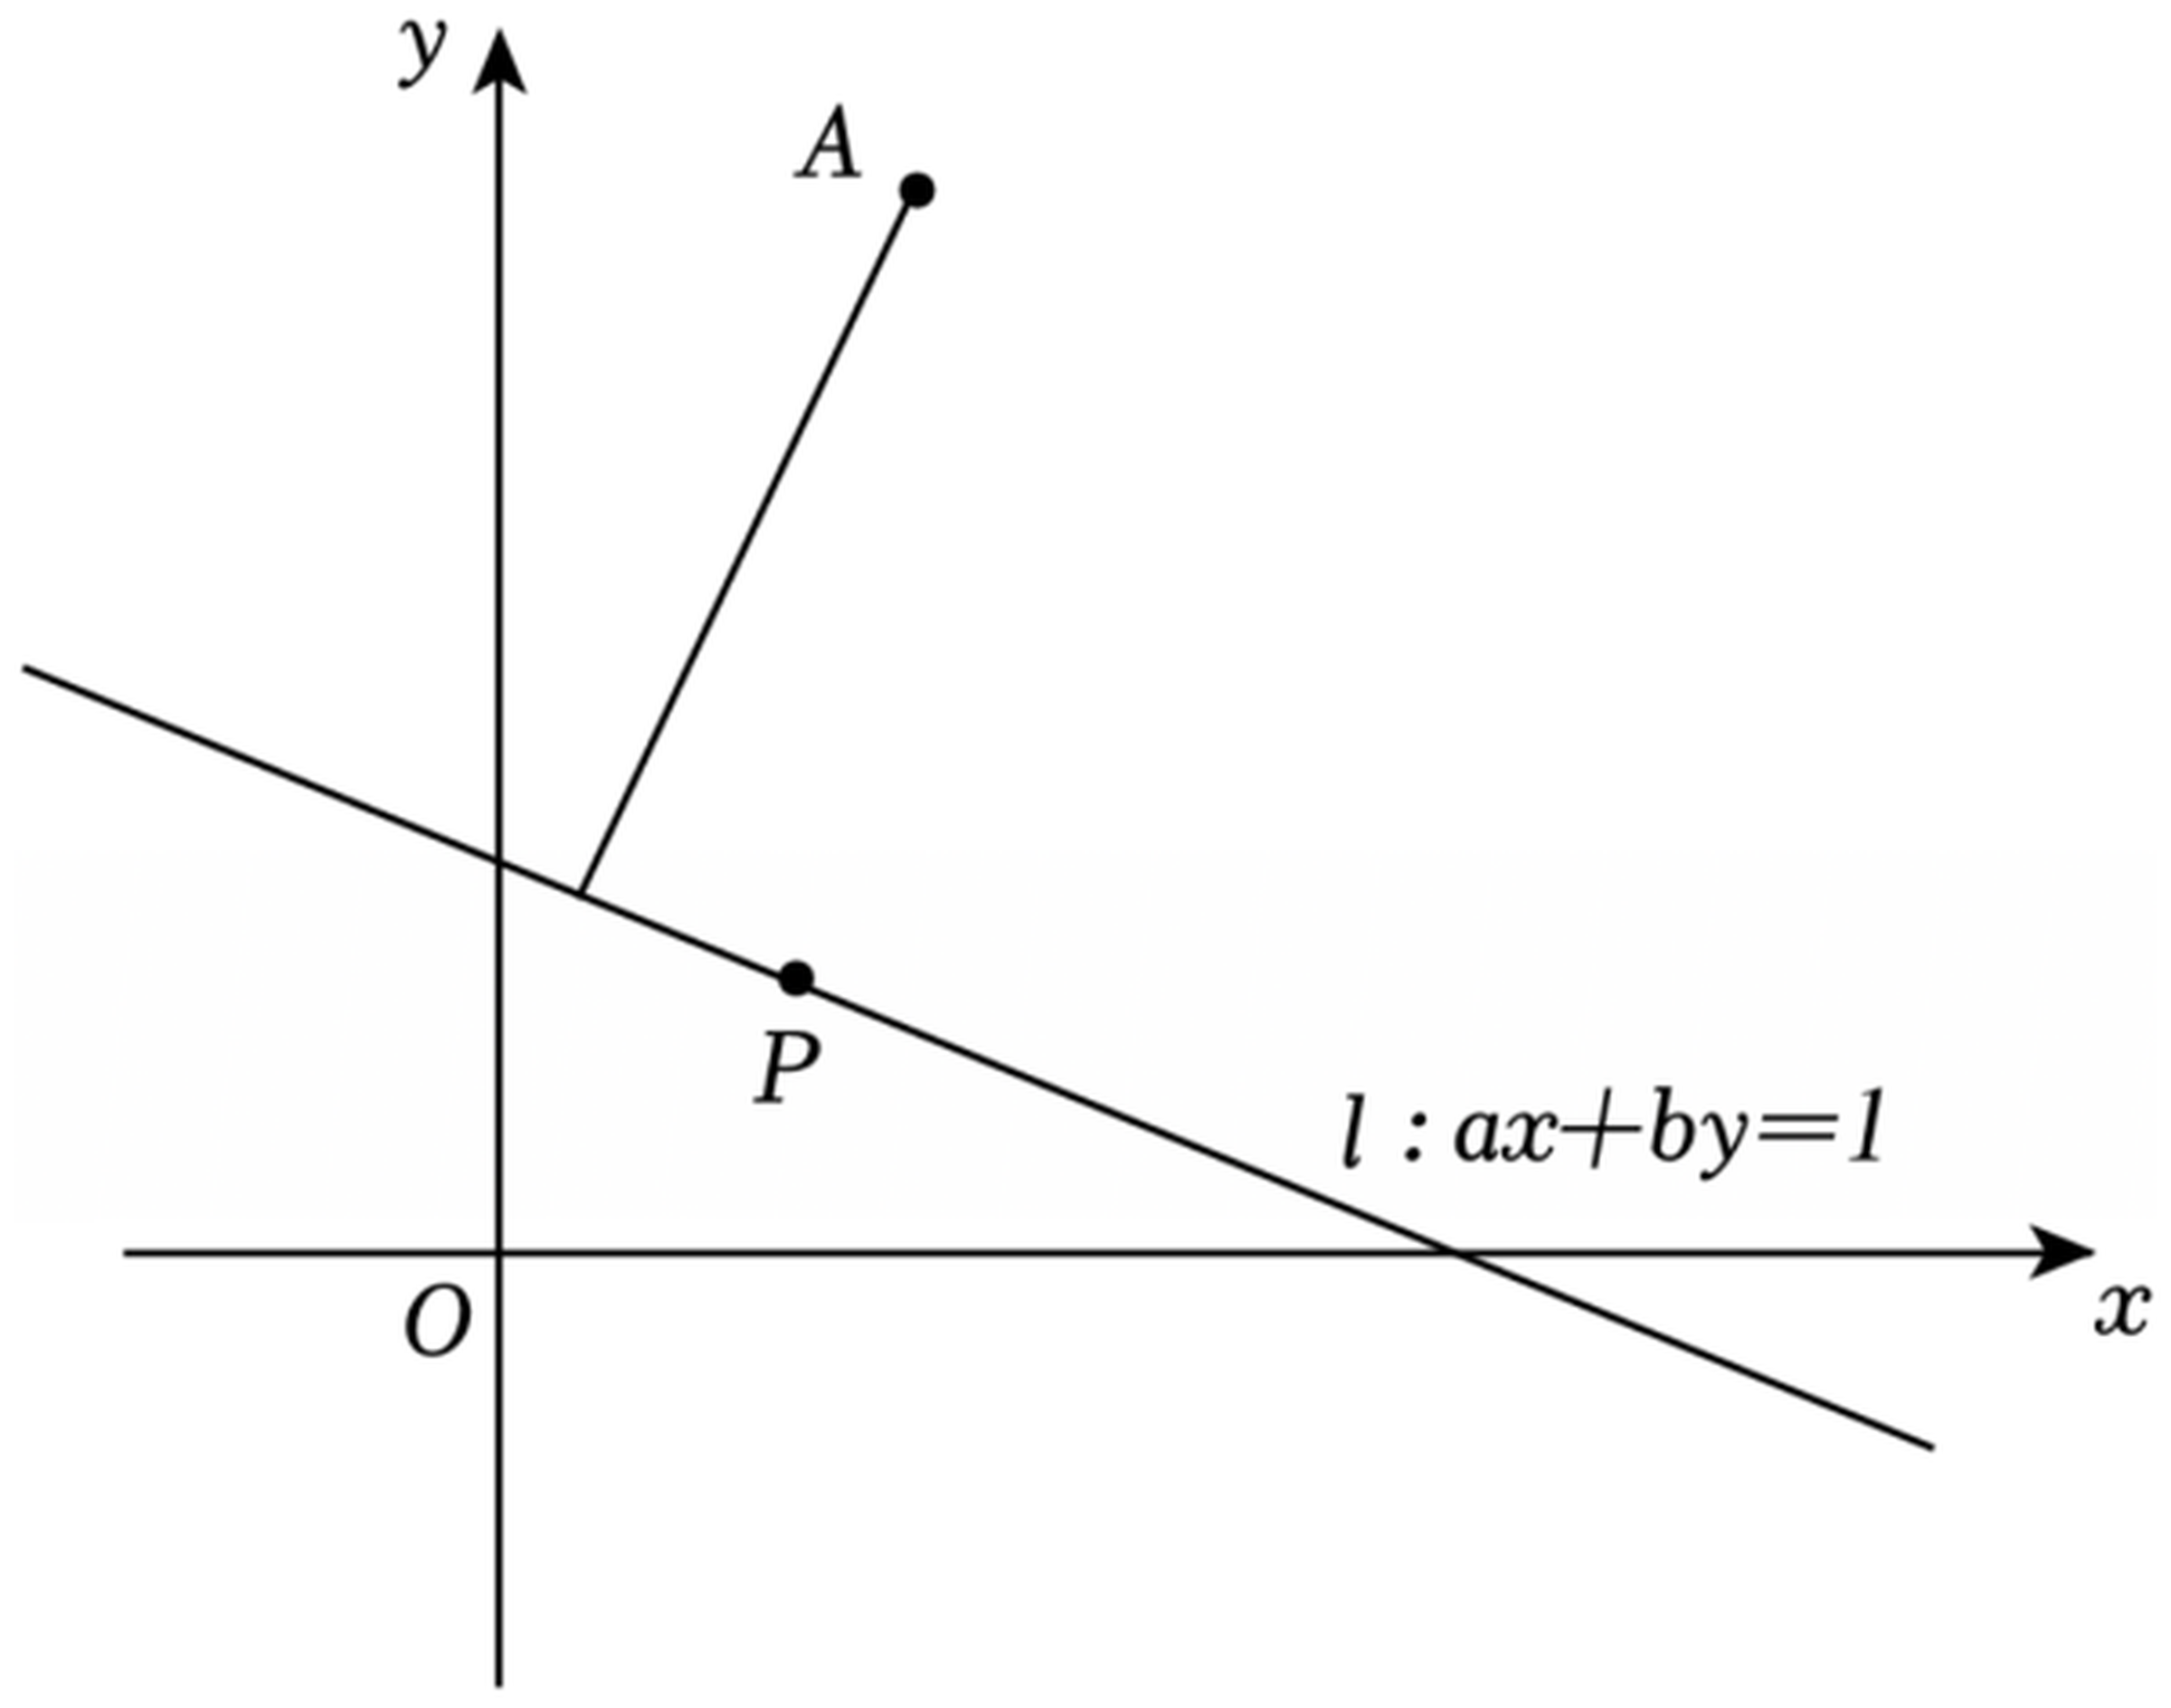
\includegraphics[width=0.56\textwidth]{figures/line_ax_plus_by_1.png}
\end{center}

\step{因为 $a+b=2$，所以直线 $l$ 恒过定点 $P\left(\dfrac12,\dfrac12\right)$，}
\step{再令 $A(1,2)$，则
$d_{A-l}=\dfrac{|a+2b-1|}{\sqrt{a^2+b^2}}\leqslant|AP|=\dfrac{\sqrt{10}}2$，}
\step{当且仅当 $l\perp AP$ 时等号成立，}
\step{又 $\dfrac{a+2b-1}{\sqrt{a^2+b^2}}\leqslant\dfrac{|a+2b-1|}{\sqrt{a^2+b^2}}$，
而当 $l\perp AP$，$a+2b-1>0$，等号也成立，}
\step{故 $\left(\dfrac{a+2b-1}{\sqrt{a^2+b^2}}\right)_{\max}=\dfrac{\sqrt{10}}2$.}
\solend

\fi

\ansspace[6]

\item （1）设 $a$、$b$、$c$ 都是正数，试证明不等式：
$\dfrac{b+c}a+\dfrac{c+a}b+\dfrac{a+b}c\geqslant6$；

（2）对一切正整数 $n$，不等式 $\dfrac{2x-1}x>\dfrac n{n+1}$ 恒成立，
则实数 $x$ 的取值范围构成的集合.

\ifanswer
\solbegin
\stepm{(1)}{因为 $a>0$，$b>0$，$c>0$，}
\step{所以 $\dfrac ba+\dfrac ab\geqslant2$，$\dfrac ca+\dfrac ac\geqslant2$，
$\dfrac cb+\dfrac bc\geqslant2$，}
\step{所以 $\left(\dfrac ba+\dfrac ab\right)+\left(\dfrac ca+\dfrac ac\right)
+\left(\dfrac cb+\dfrac bc\right)\geqslant6$，
即 $\dfrac{b+c}a+\dfrac{c+a}b+\dfrac{a+b}c\geqslant6$.}
% 注：下一行题干原卷作「……则实数 $x$ 的取值范围构成的集合.」，缺一个「求」字，
%     照抄未改，见文件头「原卷存疑」⑤。
\stepm{(2)}{考查 $y=\dfrac n{n+1}=1-\dfrac1{n+1}$，一切正整数 $n$ 函数为严格增函数，
所以 $y\geqslant\dfrac12$，}
\step{对一切正整数 $n$，不等式 $\dfrac{2x-1}x>\dfrac n{n+1}$ 恒成立，
所以 $\dfrac{2x-1}x\geqslant1$，}
\step{所以 $\dfrac{x-1}x\geqslant0$，所以 $x<0$ 或 $x\geqslant1$，}
\step{所以实数 $x$ 的取值范围是 $(-\infty,0)\cup[1,+\infty)$.}
\solend

\fi

\ansspace[6]

\end{enumerate}

\end{document}
"
% 紧凑版：xelatex "\def\iscompact{1}% 高一34_交附闵行_查漏补缺卷.tex
%   —— 高一上数学「2026-2027 年交附闵行高一上查漏补缺卷」（试卷版/答案版）
% 试卷版：xelatex 高一34_交附闵行_查漏补缺卷.tex
% 答案版：xelatex "\def\isanswer{1}\input{高一34_交附闵行_查漏补缺卷.tex}"
% 紧凑版：xelatex "\def\iscompact{1}\input{高一34_交附闵行_查漏补缺卷.tex}"
%
% 原始材料是微信公众号图文（公众号「魔都数学加油站」连载「27学年高一 34」，2026-09-25 发布，
% 原文标题「27学年高一34——2026-2027年上海市交附闵行高一上查漏补缺卷」），
% 正文为 7 张 PNG 页（均 2560×3620），取 mmbiz.qpic.cn/<hash>/0 的原图档。
% 原文本身就是一份**讲评版**，但**全卷没有任何一处印「【答案】」**——每题下方直接印【解析】，
% 答案写在解析的末句。试题文字与解析均照原卷录入，未改内容。
% 卷面的粉色斜水印属水印，未录入。
%
% 卷首标题：原卷印作「2026-2027 年交附闵行高一上查漏补缺卷」（公众号标题里的「上海市」
% 三字卷面标题行没有，本稿照卷面），年份区间按全稿惯例排 en dash，前缀照原卷保留「年」。
%
% 与原卷的排版差异（均已在 README「说明」中交代）：
%   ① 原文自**第 3 题**起（第 1、2 题未在该文中发布），故本稿题号亦自 3 起；
%   ② 原卷只有「一、填空题」「二、解答题」两个节标题（本卷无选择题），本稿照原卷分节，
%      只把标题改排成全稿统一的「大节标题」样式；
%   ③ 原卷通篇只印【解析】（无【答案】行），本稿统一改为试卷版隐去、答案版以 \ifanswer{}
%      块给出，两版彻底分离；
%   ④ 数集记号原卷两套并用：第 4 题与第 11(2) 题作斜体的 $R$，第 7 题两处作粗体的
%      $\mathbf{R}^+$，本稿按全稿惯例统一写作 $\R$；
%   ⑤ 原卷填空的横线约两个字宽，本稿按全稿惯例统一排 \blankline[4.4em]（第 9 题的第一个空
%      原卷**没有**下划线、只留了一个空格，本稿仍补出横线，见文件头「原卷存疑」①）；
%   ⑥ 原卷未印副标题，本稿按全稿惯例补出副标题「集合与常用逻辑用语」（本卷实为基本不等式
%      专题，与 高一27／高一28 同样只标主章节，见文末「高一34 专记」）；
%   ⑦ 第 13 题的配图只出现在【解析】里（题干并未写「如图」），故放进 \ifanswer 块，
%      试卷版不排；图取原卷截图、4× LANCZOS 放大（figures/line_ax_plus_by_1.png）。
%
% 原卷存疑五处（均照抄原卷、未改，见源码中该处上方注释）：
%   ① 第 9 题「则 $ab$ 的最大值为 ，」——第一个空后面只有空格、没有下划线，第二个空才有；
%   ② 第 11(2) 题题干括号内写「$a$、$b\in R$」，但函数式 $f(x)=ax^2+(3a-4)x-12$ 里并没有 $b$；
%   ③ 第 10 题只限定 $a$ 是正实数，未提 $b$ 的取值范围；
%   ④ 第 13 题题干作「求 …… 的最大值为____.」（「求」与「为」混用），且**题干未写「如图」**，
%      是【解析】里才写「如图」；
%   ⑤ 第 14(2) 题题干作「……则实数 $x$ 的取值范围构成的集合.」——缺一个「求」字。
% 另有两处标点照录：第 9 题【解析】首句末是句号、第 11(1)① 解析末句是分号。

\documentclass[a4paper,11pt]{article}
\usepackage{common}

\begin{document}

\examtitlest[3]{2026--2027 年交附闵行高一上查漏补缺卷}{集合与常用逻辑用语}

\bigsec{一、填空题}

\begin{enumerate}
\setcounter{enumi}{2}

\item 已知正实数 $m$、$n$ 满足 $\dfrac1{m+2n}+\dfrac1{2m+n}=1$，则 $m+n$ 的最小值为
\blankline[4.4em].

\ifanswer
\solbegin
\step{因为 $m$、$n\in(0,+\infty)$，$\dfrac1{m+2n}+\dfrac1{2m+n}=1$，}
\step{所以 $m+n=\dfrac13[(m+2n)+(2m+n)]\left(\dfrac1{m+2n}+\dfrac1{2m+n}\right)$}
\step{$=\dfrac13\left[2+\dfrac{2m+n}{m+2n}+\dfrac{m+2n}{2m+n}\right]
\geqslant\dfrac13\left[2+2\sqrt{\dfrac{2m+n}{m+2n}\cdot\dfrac{m+2n}{2m+n}}\right]
=\dfrac43$，}
\step{当且仅当 $\dfrac{2m+n}{m+2n}=\dfrac{m+2n}{2m+n}$，即 $m=n=\dfrac23$ 时取等号，}
\step{所以 $m+n$ 的最小值为 $\dfrac43$.}
\solend

\fi

\item 若 $a$、$b\in\R$，且 $a^2+2ab-3b^2=1$，则 $a^2+b^2$ 的最小值为 \blankline[4.4em].

\ifanswer
\solbegin
\step{由 $a^2+2ab-3b^2=1$ 得 $(a+3b)(a-b)=1$，}
\step{令 $x=a+3b$，$y=a-b$，则 $xy=1$ 且 $a=\dfrac{x+3y}4$，$b=\dfrac{x-y}4$，}
\step{所以 $a^2+b^2=\left(\dfrac{x+3y}4\right)^2+\left(\dfrac{x-y}4\right)^2
=\dfrac{x^2+5y^2+2}8\geqslant\dfrac{2\sqrt{5x^2y^2}+2}8=\dfrac{\sqrt5+1}4$，}
\step{当且仅当 $x^2=\sqrt5$，$y^2=\dfrac{\sqrt5}5$ 时取等号，
故 $a^2+b^2$ 的最小值为 $\dfrac{\sqrt5+1}4$.}
\solend

\fi

\item 已知实数 $x$、$y$ 满足 $3x^2+3y^2-2xy=4$，则 $x+y$ 的最大值为 \blankline[4.4em].

\ifanswer
\solbegin
\step{由 $3x^2+3y^2-2xy=4$，则 $3[(x+y)^2-2xy]-2xy=4$，}
\step{设 $s=x+y$，则 $3s^2-8xy=4$，即 $xy=\dfrac{3s^2-4}8$，}
\step{对任意实数 $x$、$y$，有 $xy\leqslant\left(\dfrac{x+y}2\right)^2=\dfrac{s^2}4$，
即 $\dfrac{3s^2-4}8\leqslant\dfrac{s^2}4$，}
\step{得 $s^2\leqslant4$，即 $-2\leqslant s\leqslant2$，}
\step{当 $x=y=1$ 时，满足原等式，且 $x+y=2$ 成立，因此 $x+y$ 的最大值为 $2$.}
\solend

\fi

\item 若 $a$、$b$、$c$ 都是正实数，则 $\dfrac{a^2+2b^2+4c^2}{ab+2bc}$ 的最小值为
\blankline[4.4em].

\ifanswer
\solbegin
\step{因为 $a^2+2b^2+4c^2=a^2+b^2+b^2+4c^2=(a^2+b^2)+(b^2+4c^2)\geqslant2ab+4bc$，}
\step{所以 $\dfrac{a^2+2b^2+4c^2}{ab+2bc}\geqslant\dfrac{2ab+4bc}{ab+2bc}=2$，
当且仅当 $a=b=2c$ 时取等号，}
\step{即 $\dfrac{a^2+2b^2+4c^2}{ab+2bc}$ 的最小值是 $2$.}
\solend

\fi

\item 已知 $a$、$b\in\R^+$，且 $ab=2$，则 $\dfrac b{2+a^2}+\dfrac a{2+b^2}$ 的最小值是
\blankline[4.4em].

\ifanswer
\solbegin
\step{$\dfrac b{2+a^2}+\dfrac a{2+b^2}=\dfrac b{ab+a^2}+\dfrac a{ab+b^2}
=\dfrac b{a(a+b)}+\dfrac a{b(a+b)}$}
\step{$=\dfrac{(a+b)^2-4}{2(a+b)}=\dfrac{a+b}2-\dfrac2{a+b}$，}
\step{令 $t=a+b$，则原式可设为 $y=\dfrac t2-\dfrac2t$ 的函数，}
\step{当 $t>0$ 时，此函数为严格增函数，}
\step{因为 $a$、$b\in\R^+$ 且 $ab=2$，$t=a+b\geqslant2\sqrt{ab}=2\sqrt2$，}
\step{当且仅当 $a=b=\sqrt2$ 时，$t$ 的最小值为 $2\sqrt2$，}
\step{$y=\dfrac t2-\dfrac2t$ 在 $t\in[2\sqrt2,+\infty)$ 上严格增，}
\step{所以原式的最小值为 $\dfrac{2\sqrt2}2-\dfrac2{2\sqrt2}=\dfrac{\sqrt2}2$，
则 $\dfrac b{2+a^2}+\dfrac a{2+b^2}$ 的最小值是 $\dfrac{\sqrt2}2$.}
\solend

\fi

\item 设 $x$、$y$、$z$ 为正实数，满足 $x-2y+3z=0$，则 $\dfrac{y^2}{xz}$ 的最小值是
\blankline[4.4em].

\ifanswer
\solbegin
\step{因为 $x-2y+3z=0$，所以 $y=\dfrac{x+3z}2$，}
\step{所以 $\dfrac{y^2}{xz}=\dfrac{x^2+9z^2+6xz}{4xz}\geqslant\dfrac{6xz+6xz}{4xz}=3$，
当且仅当 $x=3z$ 时取等号，}
\step{故 $\dfrac{y^2}{xz}$ 的最小值是 $3$.}
\solend

\fi

% 注：下一题的第一个空原卷只留了一个空格、**没有**下划线（第二个空才有），本稿仍按全稿
%     惯例补出横线；另其【解析】首句末原卷作句号，照录。见文件头「原卷存疑」①。
\item 设 $a$、$b$ 为正实数，且 $a+b=3$，则 $ab$ 的最大值为 \blankline[4.4em]，
$\dfrac{a^2}{a+2}+\dfrac{b^2}{b+1}$ 的最小值为 \blankline[4.4em].

\ifanswer
\solbegin
\step{因为 $a>0$，$b>0$，所以 $a+b=3\geqslant2\sqrt{ab}$，}
\step{故 $ab$ 的最大值为 $\dfrac94$，当且仅当 $a=b=\dfrac32$ 时取等号.}
\step{令 $a+2=m$，$b+1=n$，则 $m+n=a+b+3=6$，}
\step{解得 $a=m-2$，$b=n-1$，}
\step{所以 $\dfrac{a^2}{a+2}+\dfrac{b^2}{b+1}=\dfrac{(m-2)^2}m+\dfrac{(n-1)^2}n
=m+\dfrac4m+n+\dfrac1n-6=\dfrac4m+\dfrac1n$}
\step{$=\dfrac16(m+n)\left(\dfrac4m+\dfrac1n\right)
=\dfrac16\left(\dfrac{4n}m+\dfrac mn+5\right)\geqslant\dfrac16(4+5)=\dfrac32$，}
\step{当且仅当 $\dfrac{4n}m=\dfrac mn$ 时，即 $m=2n$ 时
$\dfrac{a^2}{a+2}+\dfrac{b^2}{b+1}$ 取得最小值，}
\step{因此 $\dfrac{a^2}{a+2}+\dfrac{b^2}{b+1}$ 的最小值为 $\dfrac32$.}
\solend

\fi

\item 若 $a$ 是正实数，$2a^2+3b^2=10$，则 $a\sqrt{2+b^2}$ 的最大值是 \blankline[4.4em].

\ifanswer
\solbegin
\step{$a$ 是正实数，$2a^2+3b^2=10$，变形为 $2a^2+3(b^2+2)=16$，}
\step{所以 $16\geqslant2\sqrt{2a^2\times3(b^2+2)}=2\sqrt6\cdot a\sqrt{b^2+2}$，
得 $a\sqrt{2+b^2}\leqslant\dfrac{4\sqrt6}3$，}
\step{当且仅当 $2a^2=3(b^2+2)=8$，即 $a=2$，$b^2=\dfrac23$ 时取等号，}
\step{所以 $a\sqrt{2+b^2}$ 的最大值为 $\dfrac{4\sqrt6}3$.}
\solend

\fi

\end{enumerate}

\bigsec{二、解答题}

\begin{enumerate}
\setcounter{enumi}{10}

\item （1）已知 $x>0$，$y>0$，$2xy=x+4y$. ①求 $xy$ 的最小值；②求 $x+y$ 的最小值.

（2）已知函数 $f(x)=ax^2+(3a-4)x-12$（$a$、$b\in\R$），求不等式 $f(x)\geqslant0$ 的解集.

\ifanswer
\solbegin
\stepm{(1)}{①因为 $x>0$，$y>0$，由基本不等式得
$2xy=x+4y\geqslant2\sqrt{4xy}=4\sqrt{xy}$，}
\step{解得 $xy\geqslant4$，当且仅当 $x=4y=4$ 时取等号，故 $xy$ 的最小值为 $4$；}
\step{②因为 $x>0$，$y>0$，由已知条件得 $\dfrac{4y+x}{xy}=\dfrac4x+\dfrac1y=2$，}
\step{所以 $x+y=\dfrac12(x+y)\left(\dfrac4x+\dfrac1y\right)
=\dfrac12\left(5+\dfrac{4y}x+\dfrac xy\right)
\geqslant\dfrac12\left(5+2\sqrt{\dfrac{4y}x\cdot\dfrac xy}\right)=\dfrac92$，}
\step{当且仅当 $x=2y=3$ 时，等号成立，故 $x+y$ 的最小值为 $\dfrac92$；}
% 注：下一行题干括号内原卷写「$a$、$b\in R$」，但函数式里并没有 $b$，照抄未改，
%     见文件头「原卷存疑」②。
\stepm{(2)}{当 $a=0$ 时，则 $x+3\leqslant0$，解得 $x\leqslant-3$；}
\step{当 $a\neq0$ 时，$f(x)=ax^2+(3a-4)x-12=(x+3)(ax-4)
=a(x+3)\left(x-\dfrac4a\right)$，}
\step{当 $a>0$ 时，则 $(x+3)\left(x-\dfrac4a\right)\geqslant0$，
解得 $x\leqslant-3$ 或 $x\geqslant\dfrac4a$；}
\step{当 $a<0$ 时，则 $(x+3)\left(x-\dfrac4a\right)\leqslant0$，}
\step{当 $\dfrac4a>-3$ 时，即 $a<-\dfrac43$，解 $(x+3)\left(x-\dfrac4a\right)\leqslant0$，
得 $-3\leqslant x\leqslant\dfrac4a$；}
\step{当 $\dfrac4a=-3$ 时，即 $a=-\dfrac43$，解 $(x+3)\left(x-\dfrac4a\right)\leqslant0$，
得 $x=-3$；}
\step{当 $\dfrac4a<-3$ 时，即 $-\dfrac43<a<0$，解 $(x+3)\left(x-\dfrac4a\right)\leqslant0$，
得 $\dfrac4a\leqslant x\leqslant-3$；}
\step{综上所述，当 $a<-\dfrac43$ 时，不等式 $f(x)\geqslant0$ 的解集为
$\left[-3,\dfrac4a\right]$；}
\step{当 $a=-\dfrac43$ 时，不等式 $f(x)\geqslant0$ 的解集为 $\{-3\}$；}
\step{当 $-\dfrac43<a<0$ 时，不等式 $f(x)\geqslant0$ 的解集为
$\left[\dfrac4a,-3\right]$；}
\step{当 $a=0$ 时，不等式 $f(x)\geqslant0$ 的解集为 $(-\infty,-3]$；}
\step{当 $a>0$ 时，不等式 $f(x)\geqslant0$ 的解集为
$(-\infty,-3]\cup\left[\dfrac4a,+\infty\right)$.}
\solend

\fi

\ansspace[8]

\item 已知 $x$、$y$ 都是正数，且 $\dfrac2x+\dfrac1y=1$.

\begin{enumerate}[label=(\arabic*)]
\item 求 $2x+y$ 的最小值及此时 $x$、$y$ 的取值；
\item 不等式 $(2x+y)^2\geqslant m(x+2y)$ 恒成立，求实数 $m$ 的取值范围.
\end{enumerate}

\ifanswer
\solbegin
\stepm{(1)}{$2x+y=(2x+y)\left(\dfrac2x+\dfrac1y\right)
=4+\dfrac{2x}y+\dfrac{2y}x+1\geqslant5+2\sqrt{\dfrac{2x}y\cdot\dfrac{2y}x}=9$，}
\step{当且仅当 $x=y$ 且 $\dfrac2x+\dfrac1y=1$，即 $x=y=3$ 时取等号，}
\step{此时 $2x+y$ 的最小值为 $9$.}
\stepm{(2)}{由 $\dfrac2x+\dfrac1y=1$，得 $x+2y=xy>0$，}
\step{故 $(2x+y)^2\geqslant m(x+2y)\Leftrightarrow m\leqslant\dfrac{(2x+y)^2}{x+2y}
\Leftrightarrow m\leqslant\dfrac{(2x+y)^2}{xy}$，}
\step{又 $\dfrac{(2x+y)^2}{xy}=\dfrac{4x^2+y^2+4xy}{xy}
=\dfrac{4x}y+\dfrac yx+4\geqslant2\sqrt{\dfrac{4x}y\cdot\dfrac yx}+4=8$，}
\step{当且仅当 $\begin{cases}\dfrac{4x}y=\dfrac yx\\[2pt]
\dfrac2x+\dfrac1y=1\end{cases}$ 时取等号，$\dfrac{(2x+y)^2}{xy}$ 取得最小值 $8$，}
\step{故 $m$ 的取值范围为 $\{m\mid m\leqslant8\}$.}
\solend

\fi

\ansspace[6]

% 注：本小题题干作「求 …… 的最大值为____.」（「求」与「为」混用），且**题干未写「如图」**
%     ——是【解析】里才写「如图」，照抄未改，见文件头「原卷存疑」④。
\item 已知实数 $a$、$b$ 满足 $a+b=2$，求 $\dfrac{a+2b-1}{\sqrt{a^2+b^2}}$ 的最大值为
\blankline[4.4em].

\ifanswer
\solbegin
\step{如图，考虑直线 $l:ax+by=1$，}

\begin{center}
% 图取原卷截图、4× LANCZOS 放大。图只在【解析】里出现（题干并未写「如图」），
% 故放进 \ifanswer 块，试卷版不排，见文件头⑦。
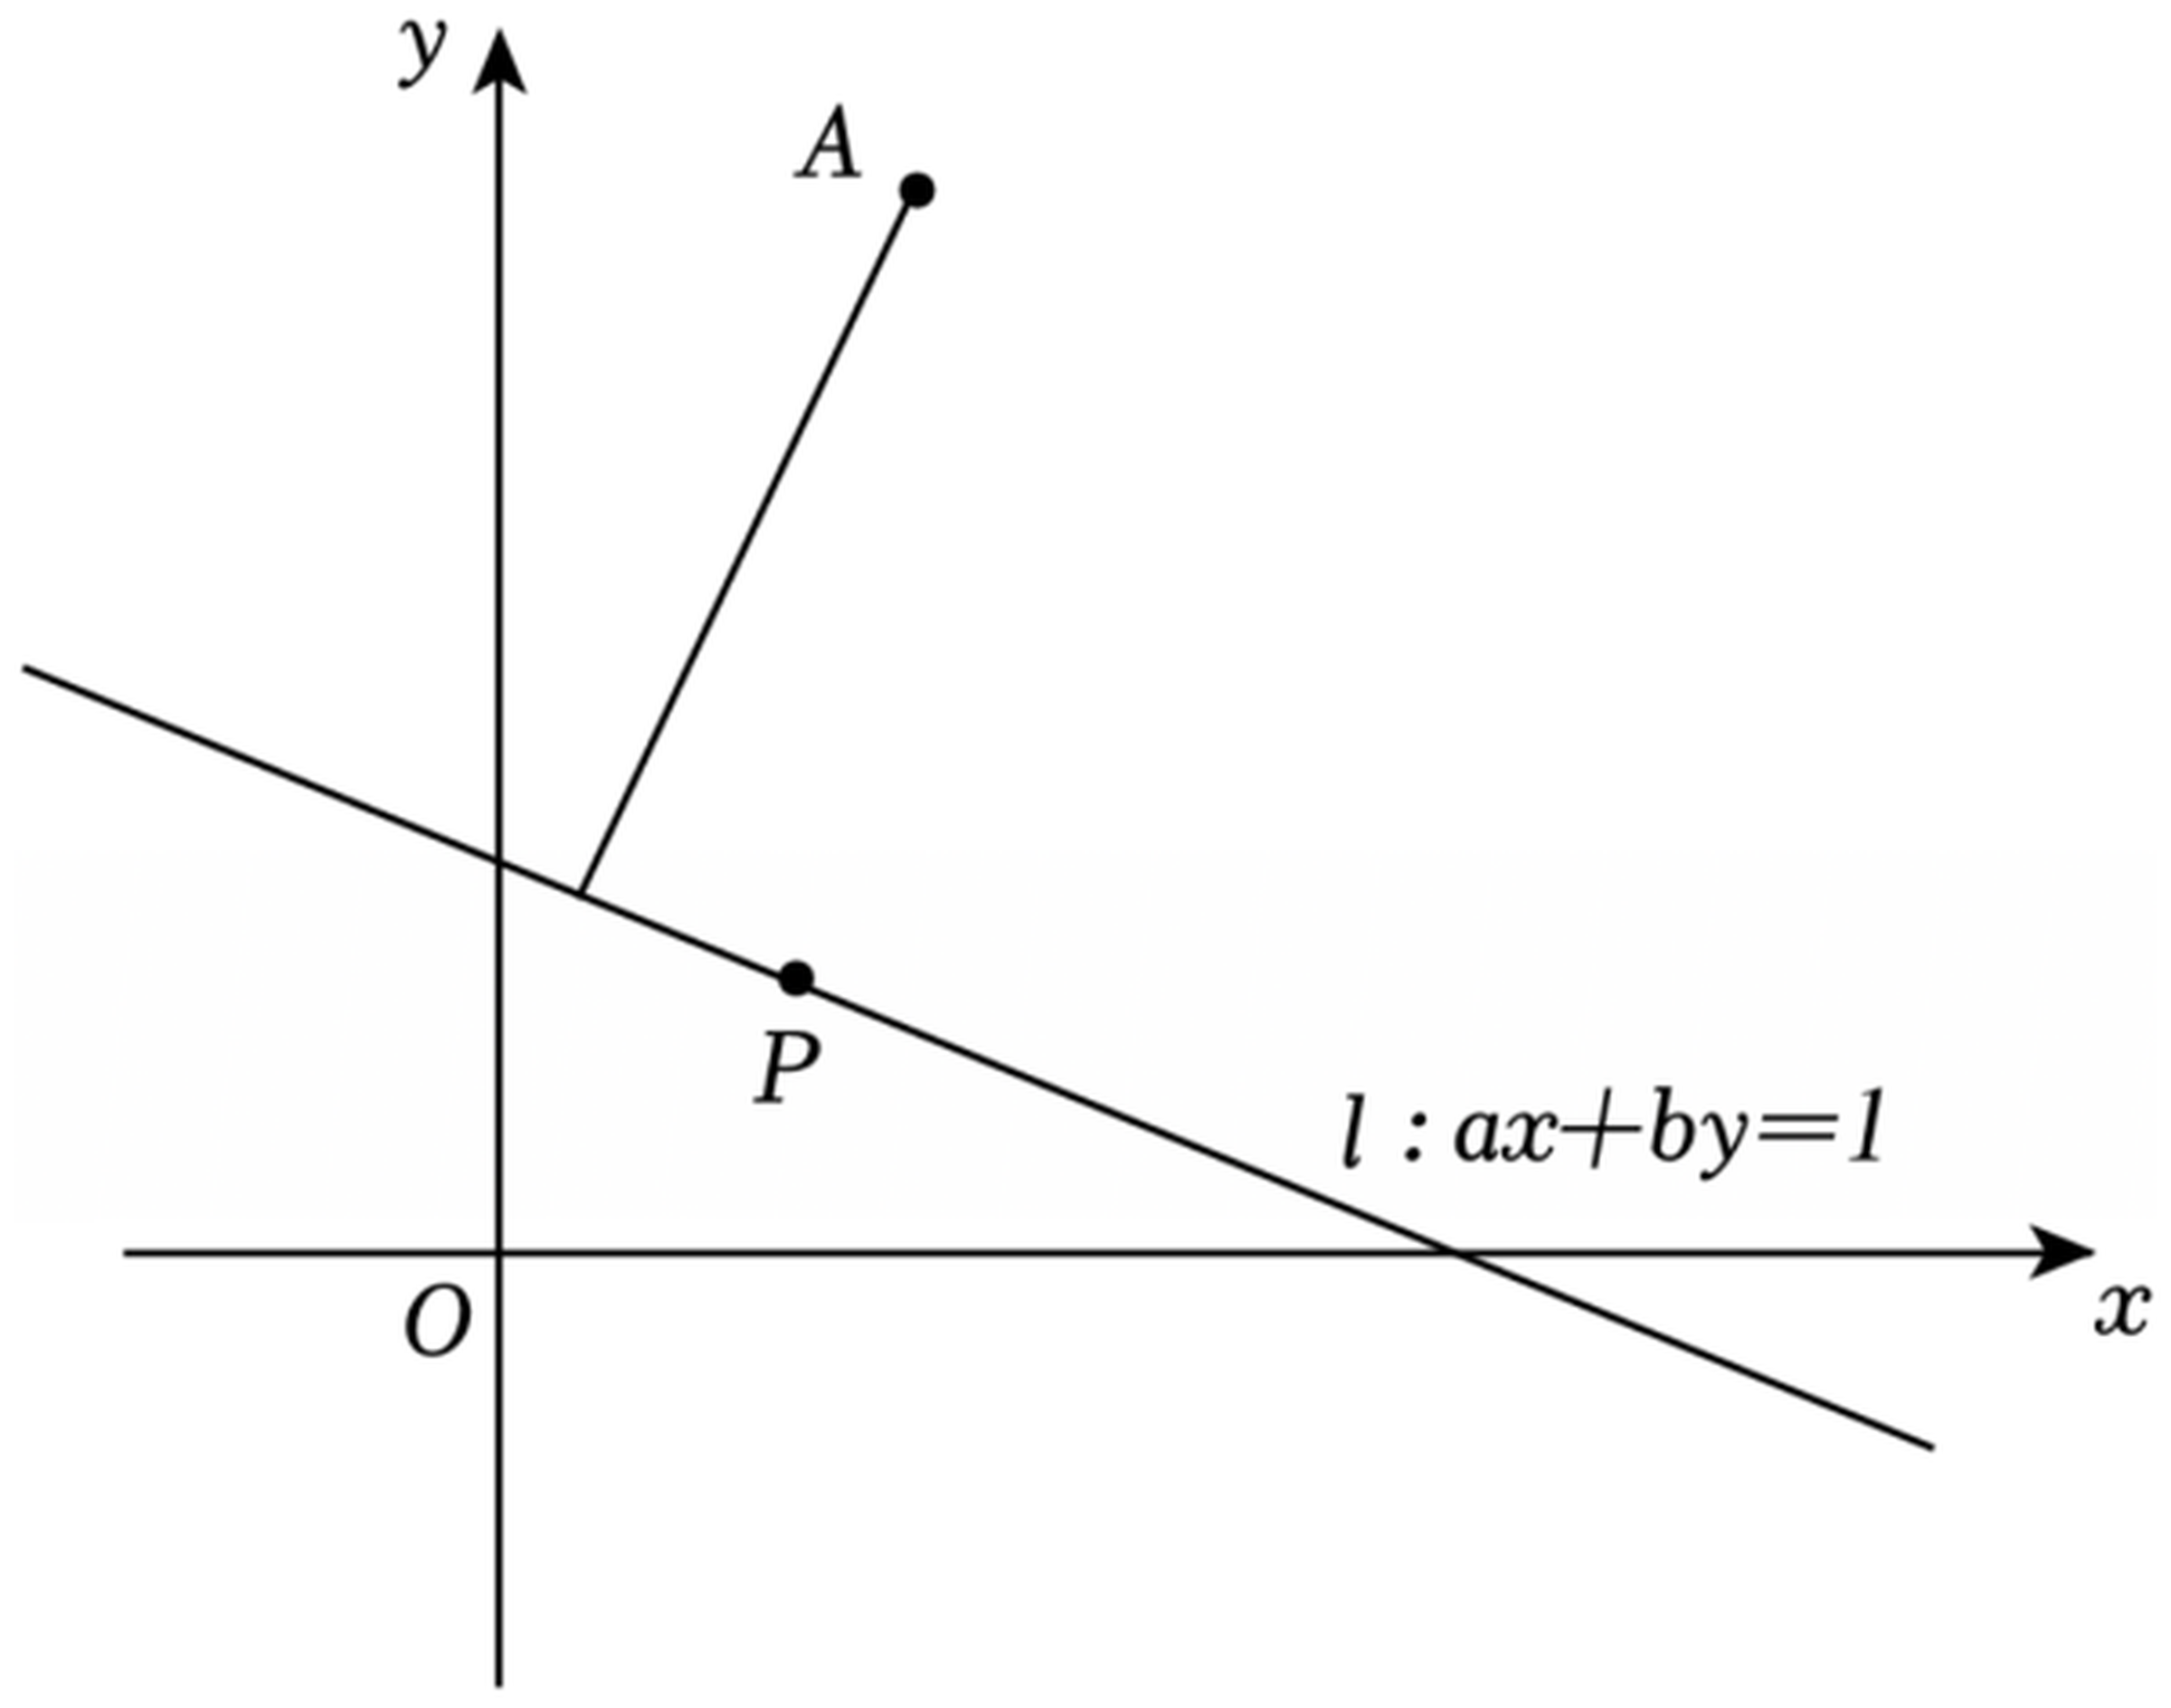
\includegraphics[width=0.56\textwidth]{figures/line_ax_plus_by_1.png}
\end{center}

\step{因为 $a+b=2$，所以直线 $l$ 恒过定点 $P\left(\dfrac12,\dfrac12\right)$，}
\step{再令 $A(1,2)$，则
$d_{A-l}=\dfrac{|a+2b-1|}{\sqrt{a^2+b^2}}\leqslant|AP|=\dfrac{\sqrt{10}}2$，}
\step{当且仅当 $l\perp AP$ 时等号成立，}
\step{又 $\dfrac{a+2b-1}{\sqrt{a^2+b^2}}\leqslant\dfrac{|a+2b-1|}{\sqrt{a^2+b^2}}$，
而当 $l\perp AP$，$a+2b-1>0$，等号也成立，}
\step{故 $\left(\dfrac{a+2b-1}{\sqrt{a^2+b^2}}\right)_{\max}=\dfrac{\sqrt{10}}2$.}
\solend

\fi

\ansspace[6]

\item （1）设 $a$、$b$、$c$ 都是正数，试证明不等式：
$\dfrac{b+c}a+\dfrac{c+a}b+\dfrac{a+b}c\geqslant6$；

（2）对一切正整数 $n$，不等式 $\dfrac{2x-1}x>\dfrac n{n+1}$ 恒成立，
则实数 $x$ 的取值范围构成的集合.

\ifanswer
\solbegin
\stepm{(1)}{因为 $a>0$，$b>0$，$c>0$，}
\step{所以 $\dfrac ba+\dfrac ab\geqslant2$，$\dfrac ca+\dfrac ac\geqslant2$，
$\dfrac cb+\dfrac bc\geqslant2$，}
\step{所以 $\left(\dfrac ba+\dfrac ab\right)+\left(\dfrac ca+\dfrac ac\right)
+\left(\dfrac cb+\dfrac bc\right)\geqslant6$，
即 $\dfrac{b+c}a+\dfrac{c+a}b+\dfrac{a+b}c\geqslant6$.}
% 注：下一行题干原卷作「……则实数 $x$ 的取值范围构成的集合.」，缺一个「求」字，
%     照抄未改，见文件头「原卷存疑」⑤。
\stepm{(2)}{考查 $y=\dfrac n{n+1}=1-\dfrac1{n+1}$，一切正整数 $n$ 函数为严格增函数，
所以 $y\geqslant\dfrac12$，}
\step{对一切正整数 $n$，不等式 $\dfrac{2x-1}x>\dfrac n{n+1}$ 恒成立，
所以 $\dfrac{2x-1}x\geqslant1$，}
\step{所以 $\dfrac{x-1}x\geqslant0$，所以 $x<0$ 或 $x\geqslant1$，}
\step{所以实数 $x$ 的取值范围是 $(-\infty,0)\cup[1,+\infty)$.}
\solend

\fi

\ansspace[6]

\end{enumerate}

\end{document}
"
%
% 原始材料是微信公众号图文（公众号「魔都数学加油站」连载「27学年高一 34」，2026-09-25 发布，
% 原文标题「27学年高一34——2026-2027年上海市交附闵行高一上查漏补缺卷」），
% 正文为 7 张 PNG 页（均 2560×3620），取 mmbiz.qpic.cn/<hash>/0 的原图档。
% 原文本身就是一份**讲评版**，但**全卷没有任何一处印「【答案】」**——每题下方直接印【解析】，
% 答案写在解析的末句。试题文字与解析均照原卷录入，未改内容。
% 卷面的粉色斜水印属水印，未录入。
%
% 卷首标题：原卷印作「2026-2027 年交附闵行高一上查漏补缺卷」（公众号标题里的「上海市」
% 三字卷面标题行没有，本稿照卷面），年份区间按全稿惯例排 en dash，前缀照原卷保留「年」。
%
% 与原卷的排版差异（均已在 README「说明」中交代）：
%   ① 原文自**第 3 题**起（第 1、2 题未在该文中发布），故本稿题号亦自 3 起；
%   ② 原卷只有「一、填空题」「二、解答题」两个节标题（本卷无选择题），本稿照原卷分节，
%      只把标题改排成全稿统一的「大节标题」样式；
%   ③ 原卷通篇只印【解析】（无【答案】行），本稿统一改为试卷版隐去、答案版以 \ifanswer{}
%      块给出，两版彻底分离；
%   ④ 数集记号原卷两套并用：第 4 题与第 11(2) 题作斜体的 $R$，第 7 题两处作粗体的
%      $\mathbf{R}^+$，本稿按全稿惯例统一写作 $\R$；
%   ⑤ 原卷填空的横线约两个字宽，本稿按全稿惯例统一排 \blankline[4.4em]（第 9 题的第一个空
%      原卷**没有**下划线、只留了一个空格，本稿仍补出横线，见文件头「原卷存疑」①）；
%   ⑥ 原卷未印副标题，本稿按全稿惯例补出副标题「集合与常用逻辑用语」（本卷实为基本不等式
%      专题，与 高一27／高一28 同样只标主章节，见文末「高一34 专记」）；
%   ⑦ 第 13 题的配图只出现在【解析】里（题干并未写「如图」），故放进 \ifanswer 块，
%      试卷版不排；图取原卷截图、4× LANCZOS 放大（figures/line_ax_plus_by_1.png）。
%
% 原卷存疑五处（均照抄原卷、未改，见源码中该处上方注释）：
%   ① 第 9 题「则 $ab$ 的最大值为 ，」——第一个空后面只有空格、没有下划线，第二个空才有；
%   ② 第 11(2) 题题干括号内写「$a$、$b\in R$」，但函数式 $f(x)=ax^2+(3a-4)x-12$ 里并没有 $b$；
%   ③ 第 10 题只限定 $a$ 是正实数，未提 $b$ 的取值范围；
%   ④ 第 13 题题干作「求 …… 的最大值为____.」（「求」与「为」混用），且**题干未写「如图」**，
%      是【解析】里才写「如图」；
%   ⑤ 第 14(2) 题题干作「……则实数 $x$ 的取值范围构成的集合.」——缺一个「求」字。
% 另有两处标点照录：第 9 题【解析】首句末是句号、第 11(1)① 解析末句是分号。

\documentclass[a4paper,11pt]{article}
\usepackage{common}

\begin{document}

\examtitlest[3]{2026--2027 年交附闵行高一上查漏补缺卷}{集合与常用逻辑用语}

\bigsec{一、填空题}

\begin{enumerate}
\setcounter{enumi}{2}

\item 已知正实数 $m$、$n$ 满足 $\dfrac1{m+2n}+\dfrac1{2m+n}=1$，则 $m+n$ 的最小值为
\blankline[4.4em].

\ifanswer
\solbegin
\step{因为 $m$、$n\in(0,+\infty)$，$\dfrac1{m+2n}+\dfrac1{2m+n}=1$，}
\step{所以 $m+n=\dfrac13[(m+2n)+(2m+n)]\left(\dfrac1{m+2n}+\dfrac1{2m+n}\right)$}
\step{$=\dfrac13\left[2+\dfrac{2m+n}{m+2n}+\dfrac{m+2n}{2m+n}\right]
\geqslant\dfrac13\left[2+2\sqrt{\dfrac{2m+n}{m+2n}\cdot\dfrac{m+2n}{2m+n}}\right]
=\dfrac43$，}
\step{当且仅当 $\dfrac{2m+n}{m+2n}=\dfrac{m+2n}{2m+n}$，即 $m=n=\dfrac23$ 时取等号，}
\step{所以 $m+n$ 的最小值为 $\dfrac43$.}
\solend

\fi

\item 若 $a$、$b\in\R$，且 $a^2+2ab-3b^2=1$，则 $a^2+b^2$ 的最小值为 \blankline[4.4em].

\ifanswer
\solbegin
\step{由 $a^2+2ab-3b^2=1$ 得 $(a+3b)(a-b)=1$，}
\step{令 $x=a+3b$，$y=a-b$，则 $xy=1$ 且 $a=\dfrac{x+3y}4$，$b=\dfrac{x-y}4$，}
\step{所以 $a^2+b^2=\left(\dfrac{x+3y}4\right)^2+\left(\dfrac{x-y}4\right)^2
=\dfrac{x^2+5y^2+2}8\geqslant\dfrac{2\sqrt{5x^2y^2}+2}8=\dfrac{\sqrt5+1}4$，}
\step{当且仅当 $x^2=\sqrt5$，$y^2=\dfrac{\sqrt5}5$ 时取等号，
故 $a^2+b^2$ 的最小值为 $\dfrac{\sqrt5+1}4$.}
\solend

\fi

\item 已知实数 $x$、$y$ 满足 $3x^2+3y^2-2xy=4$，则 $x+y$ 的最大值为 \blankline[4.4em].

\ifanswer
\solbegin
\step{由 $3x^2+3y^2-2xy=4$，则 $3[(x+y)^2-2xy]-2xy=4$，}
\step{设 $s=x+y$，则 $3s^2-8xy=4$，即 $xy=\dfrac{3s^2-4}8$，}
\step{对任意实数 $x$、$y$，有 $xy\leqslant\left(\dfrac{x+y}2\right)^2=\dfrac{s^2}4$，
即 $\dfrac{3s^2-4}8\leqslant\dfrac{s^2}4$，}
\step{得 $s^2\leqslant4$，即 $-2\leqslant s\leqslant2$，}
\step{当 $x=y=1$ 时，满足原等式，且 $x+y=2$ 成立，因此 $x+y$ 的最大值为 $2$.}
\solend

\fi

\item 若 $a$、$b$、$c$ 都是正实数，则 $\dfrac{a^2+2b^2+4c^2}{ab+2bc}$ 的最小值为
\blankline[4.4em].

\ifanswer
\solbegin
\step{因为 $a^2+2b^2+4c^2=a^2+b^2+b^2+4c^2=(a^2+b^2)+(b^2+4c^2)\geqslant2ab+4bc$，}
\step{所以 $\dfrac{a^2+2b^2+4c^2}{ab+2bc}\geqslant\dfrac{2ab+4bc}{ab+2bc}=2$，
当且仅当 $a=b=2c$ 时取等号，}
\step{即 $\dfrac{a^2+2b^2+4c^2}{ab+2bc}$ 的最小值是 $2$.}
\solend

\fi

\item 已知 $a$、$b\in\R^+$，且 $ab=2$，则 $\dfrac b{2+a^2}+\dfrac a{2+b^2}$ 的最小值是
\blankline[4.4em].

\ifanswer
\solbegin
\step{$\dfrac b{2+a^2}+\dfrac a{2+b^2}=\dfrac b{ab+a^2}+\dfrac a{ab+b^2}
=\dfrac b{a(a+b)}+\dfrac a{b(a+b)}$}
\step{$=\dfrac{(a+b)^2-4}{2(a+b)}=\dfrac{a+b}2-\dfrac2{a+b}$，}
\step{令 $t=a+b$，则原式可设为 $y=\dfrac t2-\dfrac2t$ 的函数，}
\step{当 $t>0$ 时，此函数为严格增函数，}
\step{因为 $a$、$b\in\R^+$ 且 $ab=2$，$t=a+b\geqslant2\sqrt{ab}=2\sqrt2$，}
\step{当且仅当 $a=b=\sqrt2$ 时，$t$ 的最小值为 $2\sqrt2$，}
\step{$y=\dfrac t2-\dfrac2t$ 在 $t\in[2\sqrt2,+\infty)$ 上严格增，}
\step{所以原式的最小值为 $\dfrac{2\sqrt2}2-\dfrac2{2\sqrt2}=\dfrac{\sqrt2}2$，
则 $\dfrac b{2+a^2}+\dfrac a{2+b^2}$ 的最小值是 $\dfrac{\sqrt2}2$.}
\solend

\fi

\item 设 $x$、$y$、$z$ 为正实数，满足 $x-2y+3z=0$，则 $\dfrac{y^2}{xz}$ 的最小值是
\blankline[4.4em].

\ifanswer
\solbegin
\step{因为 $x-2y+3z=0$，所以 $y=\dfrac{x+3z}2$，}
\step{所以 $\dfrac{y^2}{xz}=\dfrac{x^2+9z^2+6xz}{4xz}\geqslant\dfrac{6xz+6xz}{4xz}=3$，
当且仅当 $x=3z$ 时取等号，}
\step{故 $\dfrac{y^2}{xz}$ 的最小值是 $3$.}
\solend

\fi

% 注：下一题的第一个空原卷只留了一个空格、**没有**下划线（第二个空才有），本稿仍按全稿
%     惯例补出横线；另其【解析】首句末原卷作句号，照录。见文件头「原卷存疑」①。
\item 设 $a$、$b$ 为正实数，且 $a+b=3$，则 $ab$ 的最大值为 \blankline[4.4em]，
$\dfrac{a^2}{a+2}+\dfrac{b^2}{b+1}$ 的最小值为 \blankline[4.4em].

\ifanswer
\solbegin
\step{因为 $a>0$，$b>0$，所以 $a+b=3\geqslant2\sqrt{ab}$，}
\step{故 $ab$ 的最大值为 $\dfrac94$，当且仅当 $a=b=\dfrac32$ 时取等号.}
\step{令 $a+2=m$，$b+1=n$，则 $m+n=a+b+3=6$，}
\step{解得 $a=m-2$，$b=n-1$，}
\step{所以 $\dfrac{a^2}{a+2}+\dfrac{b^2}{b+1}=\dfrac{(m-2)^2}m+\dfrac{(n-1)^2}n
=m+\dfrac4m+n+\dfrac1n-6=\dfrac4m+\dfrac1n$}
\step{$=\dfrac16(m+n)\left(\dfrac4m+\dfrac1n\right)
=\dfrac16\left(\dfrac{4n}m+\dfrac mn+5\right)\geqslant\dfrac16(4+5)=\dfrac32$，}
\step{当且仅当 $\dfrac{4n}m=\dfrac mn$ 时，即 $m=2n$ 时
$\dfrac{a^2}{a+2}+\dfrac{b^2}{b+1}$ 取得最小值，}
\step{因此 $\dfrac{a^2}{a+2}+\dfrac{b^2}{b+1}$ 的最小值为 $\dfrac32$.}
\solend

\fi

\item 若 $a$ 是正实数，$2a^2+3b^2=10$，则 $a\sqrt{2+b^2}$ 的最大值是 \blankline[4.4em].

\ifanswer
\solbegin
\step{$a$ 是正实数，$2a^2+3b^2=10$，变形为 $2a^2+3(b^2+2)=16$，}
\step{所以 $16\geqslant2\sqrt{2a^2\times3(b^2+2)}=2\sqrt6\cdot a\sqrt{b^2+2}$，
得 $a\sqrt{2+b^2}\leqslant\dfrac{4\sqrt6}3$，}
\step{当且仅当 $2a^2=3(b^2+2)=8$，即 $a=2$，$b^2=\dfrac23$ 时取等号，}
\step{所以 $a\sqrt{2+b^2}$ 的最大值为 $\dfrac{4\sqrt6}3$.}
\solend

\fi

\end{enumerate}

\bigsec{二、解答题}

\begin{enumerate}
\setcounter{enumi}{10}

\item （1）已知 $x>0$，$y>0$，$2xy=x+4y$. ①求 $xy$ 的最小值；②求 $x+y$ 的最小值.

（2）已知函数 $f(x)=ax^2+(3a-4)x-12$（$a$、$b\in\R$），求不等式 $f(x)\geqslant0$ 的解集.

\ifanswer
\solbegin
\stepm{(1)}{①因为 $x>0$，$y>0$，由基本不等式得
$2xy=x+4y\geqslant2\sqrt{4xy}=4\sqrt{xy}$，}
\step{解得 $xy\geqslant4$，当且仅当 $x=4y=4$ 时取等号，故 $xy$ 的最小值为 $4$；}
\step{②因为 $x>0$，$y>0$，由已知条件得 $\dfrac{4y+x}{xy}=\dfrac4x+\dfrac1y=2$，}
\step{所以 $x+y=\dfrac12(x+y)\left(\dfrac4x+\dfrac1y\right)
=\dfrac12\left(5+\dfrac{4y}x+\dfrac xy\right)
\geqslant\dfrac12\left(5+2\sqrt{\dfrac{4y}x\cdot\dfrac xy}\right)=\dfrac92$，}
\step{当且仅当 $x=2y=3$ 时，等号成立，故 $x+y$ 的最小值为 $\dfrac92$；}
% 注：下一行题干括号内原卷写「$a$、$b\in R$」，但函数式里并没有 $b$，照抄未改，
%     见文件头「原卷存疑」②。
\stepm{(2)}{当 $a=0$ 时，则 $x+3\leqslant0$，解得 $x\leqslant-3$；}
\step{当 $a\neq0$ 时，$f(x)=ax^2+(3a-4)x-12=(x+3)(ax-4)
=a(x+3)\left(x-\dfrac4a\right)$，}
\step{当 $a>0$ 时，则 $(x+3)\left(x-\dfrac4a\right)\geqslant0$，
解得 $x\leqslant-3$ 或 $x\geqslant\dfrac4a$；}
\step{当 $a<0$ 时，则 $(x+3)\left(x-\dfrac4a\right)\leqslant0$，}
\step{当 $\dfrac4a>-3$ 时，即 $a<-\dfrac43$，解 $(x+3)\left(x-\dfrac4a\right)\leqslant0$，
得 $-3\leqslant x\leqslant\dfrac4a$；}
\step{当 $\dfrac4a=-3$ 时，即 $a=-\dfrac43$，解 $(x+3)\left(x-\dfrac4a\right)\leqslant0$，
得 $x=-3$；}
\step{当 $\dfrac4a<-3$ 时，即 $-\dfrac43<a<0$，解 $(x+3)\left(x-\dfrac4a\right)\leqslant0$，
得 $\dfrac4a\leqslant x\leqslant-3$；}
\step{综上所述，当 $a<-\dfrac43$ 时，不等式 $f(x)\geqslant0$ 的解集为
$\left[-3,\dfrac4a\right]$；}
\step{当 $a=-\dfrac43$ 时，不等式 $f(x)\geqslant0$ 的解集为 $\{-3\}$；}
\step{当 $-\dfrac43<a<0$ 时，不等式 $f(x)\geqslant0$ 的解集为
$\left[\dfrac4a,-3\right]$；}
\step{当 $a=0$ 时，不等式 $f(x)\geqslant0$ 的解集为 $(-\infty,-3]$；}
\step{当 $a>0$ 时，不等式 $f(x)\geqslant0$ 的解集为
$(-\infty,-3]\cup\left[\dfrac4a,+\infty\right)$.}
\solend

\fi

\ansspace[8]

\item 已知 $x$、$y$ 都是正数，且 $\dfrac2x+\dfrac1y=1$.

\begin{enumerate}[label=(\arabic*)]
\item 求 $2x+y$ 的最小值及此时 $x$、$y$ 的取值；
\item 不等式 $(2x+y)^2\geqslant m(x+2y)$ 恒成立，求实数 $m$ 的取值范围.
\end{enumerate}

\ifanswer
\solbegin
\stepm{(1)}{$2x+y=(2x+y)\left(\dfrac2x+\dfrac1y\right)
=4+\dfrac{2x}y+\dfrac{2y}x+1\geqslant5+2\sqrt{\dfrac{2x}y\cdot\dfrac{2y}x}=9$，}
\step{当且仅当 $x=y$ 且 $\dfrac2x+\dfrac1y=1$，即 $x=y=3$ 时取等号，}
\step{此时 $2x+y$ 的最小值为 $9$.}
\stepm{(2)}{由 $\dfrac2x+\dfrac1y=1$，得 $x+2y=xy>0$，}
\step{故 $(2x+y)^2\geqslant m(x+2y)\Leftrightarrow m\leqslant\dfrac{(2x+y)^2}{x+2y}
\Leftrightarrow m\leqslant\dfrac{(2x+y)^2}{xy}$，}
\step{又 $\dfrac{(2x+y)^2}{xy}=\dfrac{4x^2+y^2+4xy}{xy}
=\dfrac{4x}y+\dfrac yx+4\geqslant2\sqrt{\dfrac{4x}y\cdot\dfrac yx}+4=8$，}
\step{当且仅当 $\begin{cases}\dfrac{4x}y=\dfrac yx\\[2pt]
\dfrac2x+\dfrac1y=1\end{cases}$ 时取等号，$\dfrac{(2x+y)^2}{xy}$ 取得最小值 $8$，}
\step{故 $m$ 的取值范围为 $\{m\mid m\leqslant8\}$.}
\solend

\fi

\ansspace[6]

% 注：本小题题干作「求 …… 的最大值为____.」（「求」与「为」混用），且**题干未写「如图」**
%     ——是【解析】里才写「如图」，照抄未改，见文件头「原卷存疑」④。
\item 已知实数 $a$、$b$ 满足 $a+b=2$，求 $\dfrac{a+2b-1}{\sqrt{a^2+b^2}}$ 的最大值为
\blankline[4.4em].

\ifanswer
\solbegin
\step{如图，考虑直线 $l:ax+by=1$，}

\begin{center}
% 图取原卷截图、4× LANCZOS 放大。图只在【解析】里出现（题干并未写「如图」），
% 故放进 \ifanswer 块，试卷版不排，见文件头⑦。
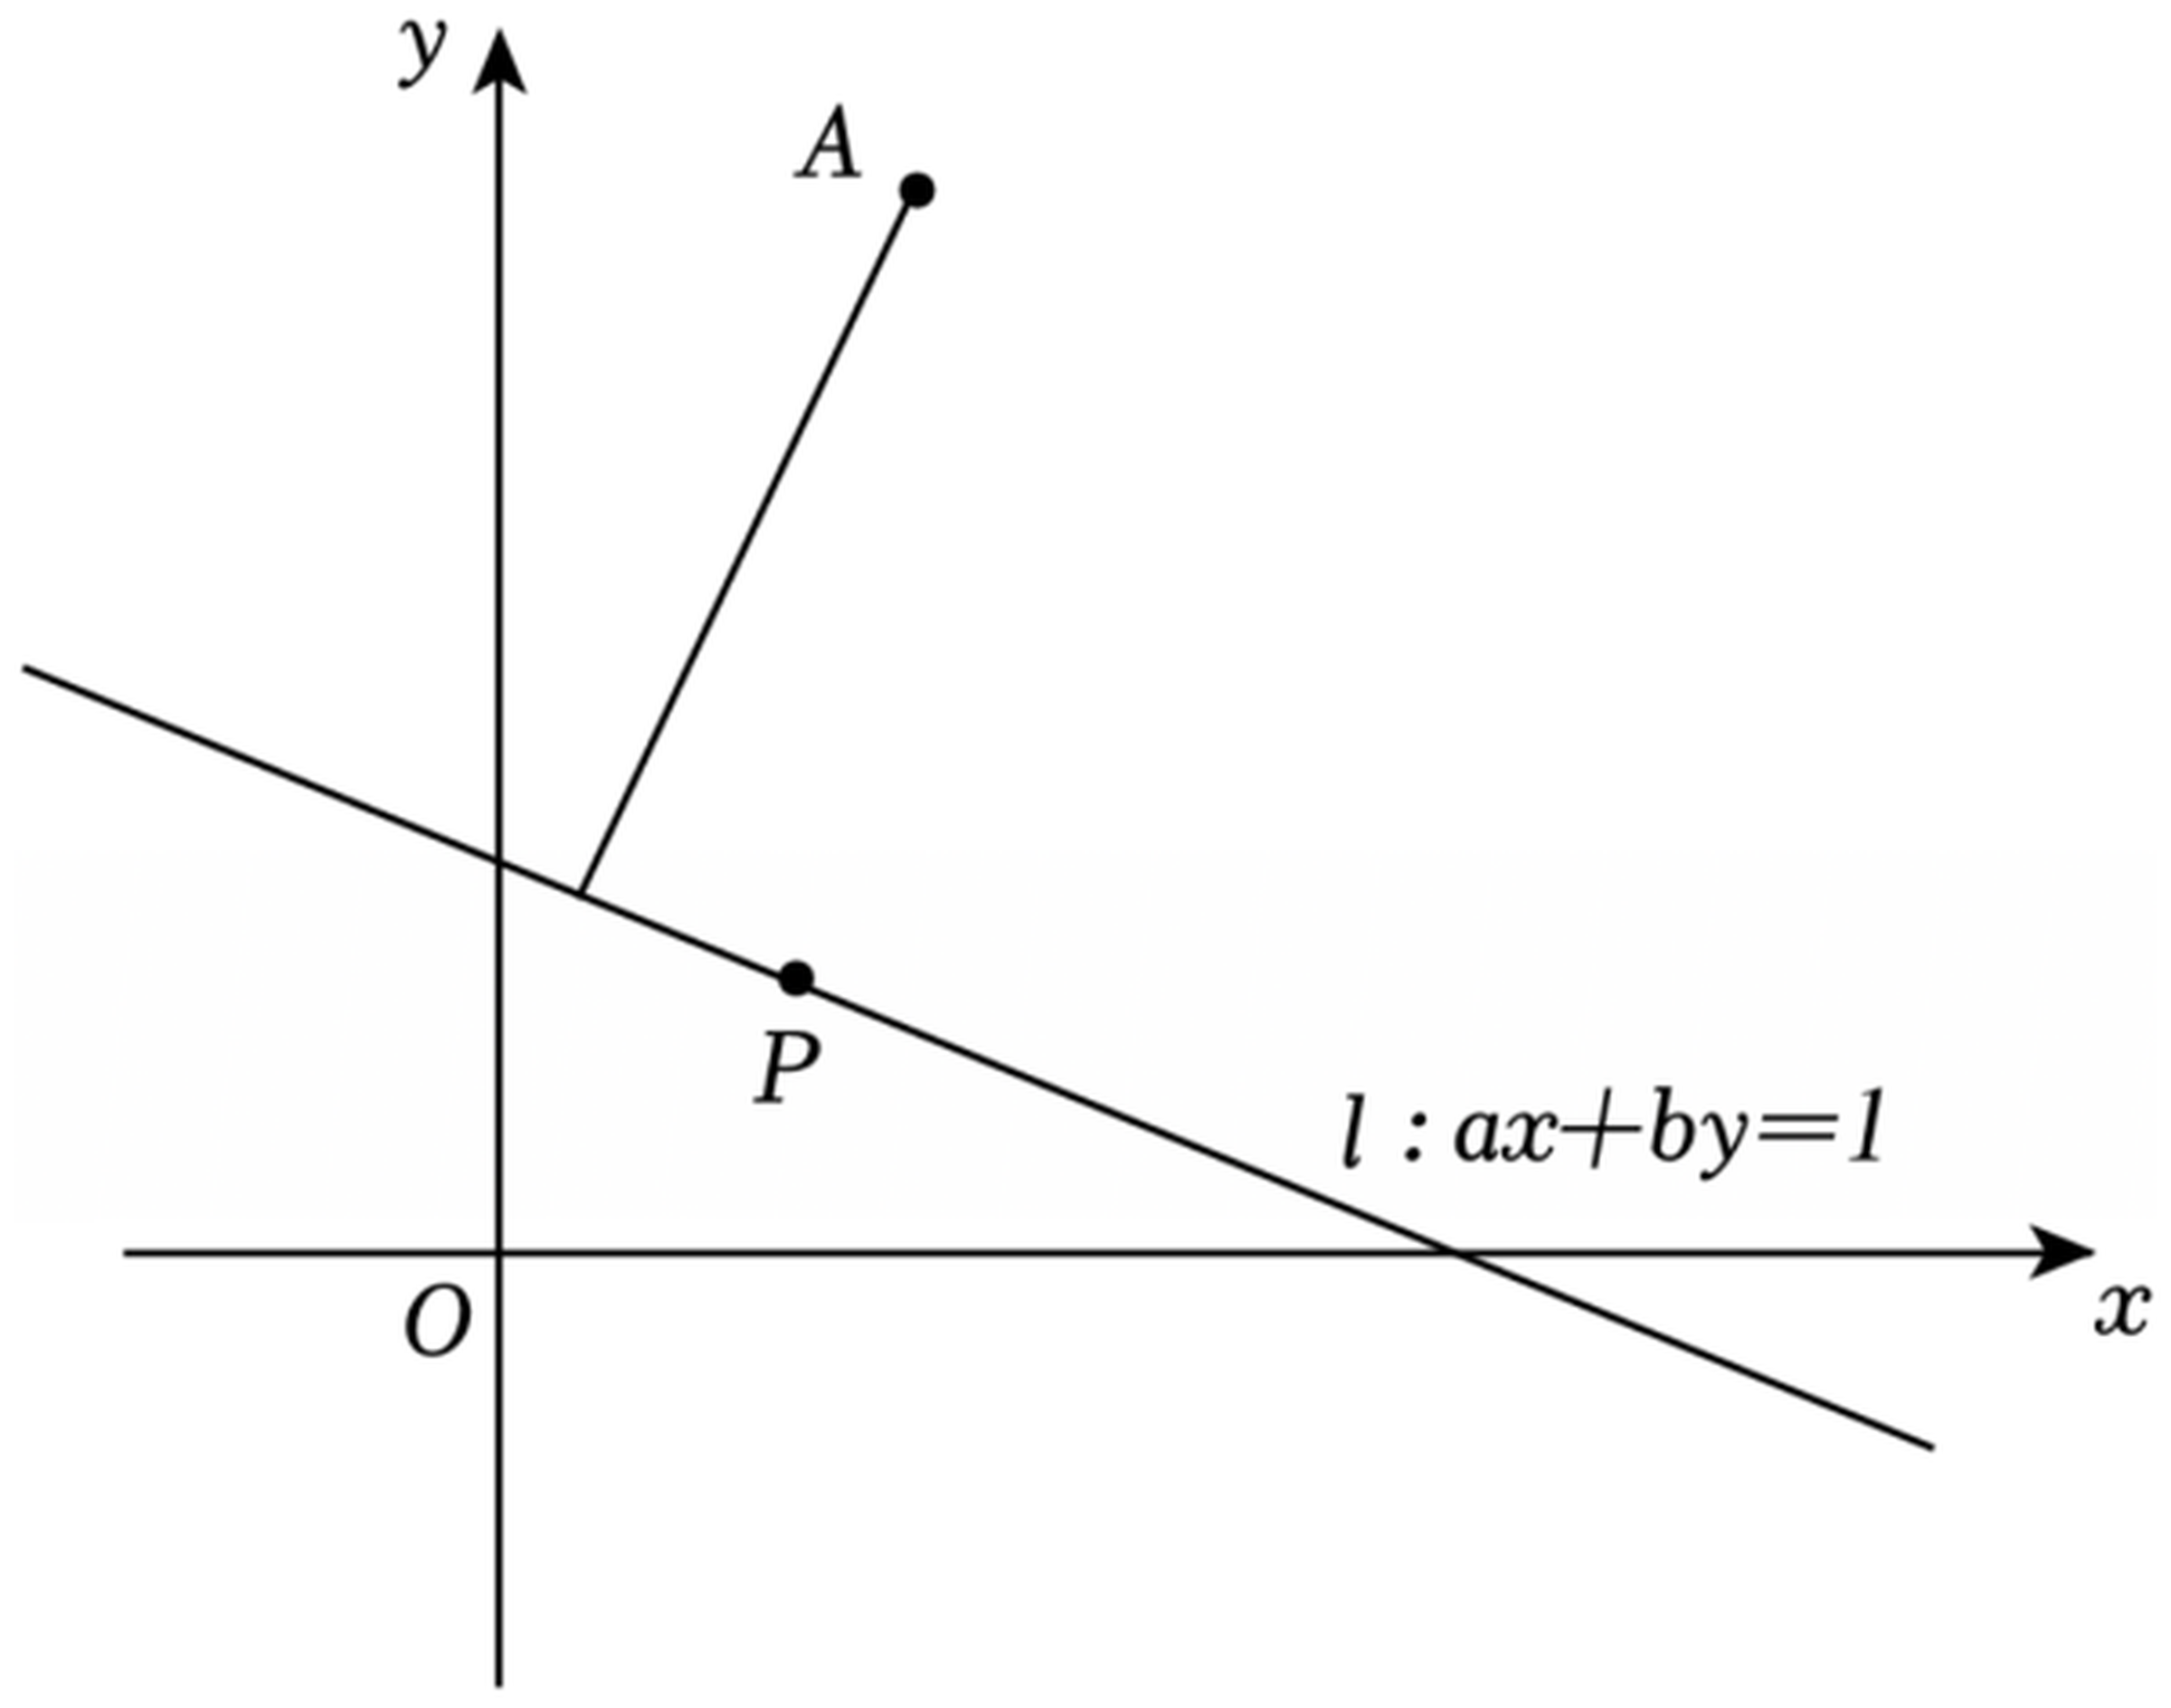
\includegraphics[width=0.56\textwidth]{figures/line_ax_plus_by_1.png}
\end{center}

\step{因为 $a+b=2$，所以直线 $l$ 恒过定点 $P\left(\dfrac12,\dfrac12\right)$，}
\step{再令 $A(1,2)$，则
$d_{A-l}=\dfrac{|a+2b-1|}{\sqrt{a^2+b^2}}\leqslant|AP|=\dfrac{\sqrt{10}}2$，}
\step{当且仅当 $l\perp AP$ 时等号成立，}
\step{又 $\dfrac{a+2b-1}{\sqrt{a^2+b^2}}\leqslant\dfrac{|a+2b-1|}{\sqrt{a^2+b^2}}$，
而当 $l\perp AP$，$a+2b-1>0$，等号也成立，}
\step{故 $\left(\dfrac{a+2b-1}{\sqrt{a^2+b^2}}\right)_{\max}=\dfrac{\sqrt{10}}2$.}
\solend

\fi

\ansspace[6]

\item （1）设 $a$、$b$、$c$ 都是正数，试证明不等式：
$\dfrac{b+c}a+\dfrac{c+a}b+\dfrac{a+b}c\geqslant6$；

（2）对一切正整数 $n$，不等式 $\dfrac{2x-1}x>\dfrac n{n+1}$ 恒成立，
则实数 $x$ 的取值范围构成的集合.

\ifanswer
\solbegin
\stepm{(1)}{因为 $a>0$，$b>0$，$c>0$，}
\step{所以 $\dfrac ba+\dfrac ab\geqslant2$，$\dfrac ca+\dfrac ac\geqslant2$，
$\dfrac cb+\dfrac bc\geqslant2$，}
\step{所以 $\left(\dfrac ba+\dfrac ab\right)+\left(\dfrac ca+\dfrac ac\right)
+\left(\dfrac cb+\dfrac bc\right)\geqslant6$，
即 $\dfrac{b+c}a+\dfrac{c+a}b+\dfrac{a+b}c\geqslant6$.}
% 注：下一行题干原卷作「……则实数 $x$ 的取值范围构成的集合.」，缺一个「求」字，
%     照抄未改，见文件头「原卷存疑」⑤。
\stepm{(2)}{考查 $y=\dfrac n{n+1}=1-\dfrac1{n+1}$，一切正整数 $n$ 函数为严格增函数，
所以 $y\geqslant\dfrac12$，}
\step{对一切正整数 $n$，不等式 $\dfrac{2x-1}x>\dfrac n{n+1}$ 恒成立，
所以 $\dfrac{2x-1}x\geqslant1$，}
\step{所以 $\dfrac{x-1}x\geqslant0$，所以 $x<0$ 或 $x\geqslant1$，}
\step{所以实数 $x$ 的取值范围是 $(-\infty,0)\cup[1,+\infty)$.}
\solend

\fi

\ansspace[6]

\end{enumerate}

\end{document}
"
%
% 原始材料是微信公众号图文（公众号「魔都数学加油站」连载「27学年高一 34」，2026-09-25 发布，
% 原文标题「27学年高一34——2026-2027年上海市交附闵行高一上查漏补缺卷」），
% 正文为 7 张 PNG 页（均 2560×3620），取 mmbiz.qpic.cn/<hash>/0 的原图档。
% 原文本身就是一份**讲评版**，但**全卷没有任何一处印「【答案】」**——每题下方直接印【解析】，
% 答案写在解析的末句。试题文字与解析均照原卷录入，未改内容。
% 卷面的粉色斜水印属水印，未录入。
%
% 卷首标题：原卷印作「2026-2027 年交附闵行高一上查漏补缺卷」（公众号标题里的「上海市」
% 三字卷面标题行没有，本稿照卷面），年份区间按全稿惯例排 en dash，前缀照原卷保留「年」。
%
% 与原卷的排版差异（均已在 README「说明」中交代）：
%   ① 原文自**第 3 题**起（第 1、2 题未在该文中发布），故本稿题号亦自 3 起；
%   ② 原卷只有「一、填空题」「二、解答题」两个节标题（本卷无选择题），本稿照原卷分节，
%      只把标题改排成全稿统一的「大节标题」样式；
%   ③ 原卷通篇只印【解析】（无【答案】行），本稿统一改为试卷版隐去、答案版以 \ifanswer{}
%      块给出，两版彻底分离；
%   ④ 数集记号原卷两套并用：第 4 题与第 11(2) 题作斜体的 $R$，第 7 题两处作粗体的
%      $\mathbf{R}^+$，本稿按全稿惯例统一写作 $\R$；
%   ⑤ 原卷填空的横线约两个字宽，本稿按全稿惯例统一排 \blankline[4.4em]（第 9 题的第一个空
%      原卷**没有**下划线、只留了一个空格，本稿仍补出横线，见文件头「原卷存疑」①）；
%   ⑥ 原卷未印副标题，本稿按全稿惯例补出副标题「集合与常用逻辑用语」（本卷实为基本不等式
%      专题，与 高一27／高一28 同样只标主章节，见文末「高一34 专记」）；
%   ⑦ 第 13 题的配图只出现在【解析】里（题干并未写「如图」），故放进 \ifanswer 块，
%      试卷版不排；图取原卷截图、4× LANCZOS 放大（figures/line_ax_plus_by_1.png）。
%
% 原卷存疑五处（均照抄原卷、未改，见源码中该处上方注释）：
%   ① 第 9 题「则 $ab$ 的最大值为 ，」——第一个空后面只有空格、没有下划线，第二个空才有；
%   ② 第 11(2) 题题干括号内写「$a$、$b\in R$」，但函数式 $f(x)=ax^2+(3a-4)x-12$ 里并没有 $b$；
%   ③ 第 10 题只限定 $a$ 是正实数，未提 $b$ 的取值范围；
%   ④ 第 13 题题干作「求 …… 的最大值为____.」（「求」与「为」混用），且**题干未写「如图」**，
%      是【解析】里才写「如图」；
%   ⑤ 第 14(2) 题题干作「……则实数 $x$ 的取值范围构成的集合.」——缺一个「求」字。
% 另有两处标点照录：第 9 题【解析】首句末是句号、第 11(1)① 解析末句是分号。

\documentclass[a4paper,11pt]{article}
\usepackage{common}

\begin{document}

\examtitlest[3]{2026--2027 年交附闵行高一上查漏补缺卷}{集合与常用逻辑用语}

\bigsec{一、填空题}

\begin{enumerate}
\setcounter{enumi}{2}

\item 已知正实数 $m$、$n$ 满足 $\dfrac1{m+2n}+\dfrac1{2m+n}=1$，则 $m+n$ 的最小值为
\blankline[4.4em].

\ifanswer
\solbegin
\step{因为 $m$、$n\in(0,+\infty)$，$\dfrac1{m+2n}+\dfrac1{2m+n}=1$，}
\step{所以 $m+n=\dfrac13[(m+2n)+(2m+n)]\left(\dfrac1{m+2n}+\dfrac1{2m+n}\right)$}
\step{$=\dfrac13\left[2+\dfrac{2m+n}{m+2n}+\dfrac{m+2n}{2m+n}\right]
\geqslant\dfrac13\left[2+2\sqrt{\dfrac{2m+n}{m+2n}\cdot\dfrac{m+2n}{2m+n}}\right]
=\dfrac43$，}
\step{当且仅当 $\dfrac{2m+n}{m+2n}=\dfrac{m+2n}{2m+n}$，即 $m=n=\dfrac23$ 时取等号，}
\step{所以 $m+n$ 的最小值为 $\dfrac43$.}
\solend

\fi

\item 若 $a$、$b\in\R$，且 $a^2+2ab-3b^2=1$，则 $a^2+b^2$ 的最小值为 \blankline[4.4em].

\ifanswer
\solbegin
\step{由 $a^2+2ab-3b^2=1$ 得 $(a+3b)(a-b)=1$，}
\step{令 $x=a+3b$，$y=a-b$，则 $xy=1$ 且 $a=\dfrac{x+3y}4$，$b=\dfrac{x-y}4$，}
\step{所以 $a^2+b^2=\left(\dfrac{x+3y}4\right)^2+\left(\dfrac{x-y}4\right)^2
=\dfrac{x^2+5y^2+2}8\geqslant\dfrac{2\sqrt{5x^2y^2}+2}8=\dfrac{\sqrt5+1}4$，}
\step{当且仅当 $x^2=\sqrt5$，$y^2=\dfrac{\sqrt5}5$ 时取等号，
故 $a^2+b^2$ 的最小值为 $\dfrac{\sqrt5+1}4$.}
\solend

\fi

\item 已知实数 $x$、$y$ 满足 $3x^2+3y^2-2xy=4$，则 $x+y$ 的最大值为 \blankline[4.4em].

\ifanswer
\solbegin
\step{由 $3x^2+3y^2-2xy=4$，则 $3[(x+y)^2-2xy]-2xy=4$，}
\step{设 $s=x+y$，则 $3s^2-8xy=4$，即 $xy=\dfrac{3s^2-4}8$，}
\step{对任意实数 $x$、$y$，有 $xy\leqslant\left(\dfrac{x+y}2\right)^2=\dfrac{s^2}4$，
即 $\dfrac{3s^2-4}8\leqslant\dfrac{s^2}4$，}
\step{得 $s^2\leqslant4$，即 $-2\leqslant s\leqslant2$，}
\step{当 $x=y=1$ 时，满足原等式，且 $x+y=2$ 成立，因此 $x+y$ 的最大值为 $2$.}
\solend

\fi

\item 若 $a$、$b$、$c$ 都是正实数，则 $\dfrac{a^2+2b^2+4c^2}{ab+2bc}$ 的最小值为
\blankline[4.4em].

\ifanswer
\solbegin
\step{因为 $a^2+2b^2+4c^2=a^2+b^2+b^2+4c^2=(a^2+b^2)+(b^2+4c^2)\geqslant2ab+4bc$，}
\step{所以 $\dfrac{a^2+2b^2+4c^2}{ab+2bc}\geqslant\dfrac{2ab+4bc}{ab+2bc}=2$，
当且仅当 $a=b=2c$ 时取等号，}
\step{即 $\dfrac{a^2+2b^2+4c^2}{ab+2bc}$ 的最小值是 $2$.}
\solend

\fi

\item 已知 $a$、$b\in\R^+$，且 $ab=2$，则 $\dfrac b{2+a^2}+\dfrac a{2+b^2}$ 的最小值是
\blankline[4.4em].

\ifanswer
\solbegin
\step{$\dfrac b{2+a^2}+\dfrac a{2+b^2}=\dfrac b{ab+a^2}+\dfrac a{ab+b^2}
=\dfrac b{a(a+b)}+\dfrac a{b(a+b)}$}
\step{$=\dfrac{(a+b)^2-4}{2(a+b)}=\dfrac{a+b}2-\dfrac2{a+b}$，}
\step{令 $t=a+b$，则原式可设为 $y=\dfrac t2-\dfrac2t$ 的函数，}
\step{当 $t>0$ 时，此函数为严格增函数，}
\step{因为 $a$、$b\in\R^+$ 且 $ab=2$，$t=a+b\geqslant2\sqrt{ab}=2\sqrt2$，}
\step{当且仅当 $a=b=\sqrt2$ 时，$t$ 的最小值为 $2\sqrt2$，}
\step{$y=\dfrac t2-\dfrac2t$ 在 $t\in[2\sqrt2,+\infty)$ 上严格增，}
\step{所以原式的最小值为 $\dfrac{2\sqrt2}2-\dfrac2{2\sqrt2}=\dfrac{\sqrt2}2$，
则 $\dfrac b{2+a^2}+\dfrac a{2+b^2}$ 的最小值是 $\dfrac{\sqrt2}2$.}
\solend

\fi

\item 设 $x$、$y$、$z$ 为正实数，满足 $x-2y+3z=0$，则 $\dfrac{y^2}{xz}$ 的最小值是
\blankline[4.4em].

\ifanswer
\solbegin
\step{因为 $x-2y+3z=0$，所以 $y=\dfrac{x+3z}2$，}
\step{所以 $\dfrac{y^2}{xz}=\dfrac{x^2+9z^2+6xz}{4xz}\geqslant\dfrac{6xz+6xz}{4xz}=3$，
当且仅当 $x=3z$ 时取等号，}
\step{故 $\dfrac{y^2}{xz}$ 的最小值是 $3$.}
\solend

\fi

% 注：下一题的第一个空原卷只留了一个空格、**没有**下划线（第二个空才有），本稿仍按全稿
%     惯例补出横线；另其【解析】首句末原卷作句号，照录。见文件头「原卷存疑」①。
\item 设 $a$、$b$ 为正实数，且 $a+b=3$，则 $ab$ 的最大值为 \blankline[4.4em]，
$\dfrac{a^2}{a+2}+\dfrac{b^2}{b+1}$ 的最小值为 \blankline[4.4em].

\ifanswer
\solbegin
\step{因为 $a>0$，$b>0$，所以 $a+b=3\geqslant2\sqrt{ab}$，}
\step{故 $ab$ 的最大值为 $\dfrac94$，当且仅当 $a=b=\dfrac32$ 时取等号.}
\step{令 $a+2=m$，$b+1=n$，则 $m+n=a+b+3=6$，}
\step{解得 $a=m-2$，$b=n-1$，}
\step{所以 $\dfrac{a^2}{a+2}+\dfrac{b^2}{b+1}=\dfrac{(m-2)^2}m+\dfrac{(n-1)^2}n
=m+\dfrac4m+n+\dfrac1n-6=\dfrac4m+\dfrac1n$}
\step{$=\dfrac16(m+n)\left(\dfrac4m+\dfrac1n\right)
=\dfrac16\left(\dfrac{4n}m+\dfrac mn+5\right)\geqslant\dfrac16(4+5)=\dfrac32$，}
\step{当且仅当 $\dfrac{4n}m=\dfrac mn$ 时，即 $m=2n$ 时
$\dfrac{a^2}{a+2}+\dfrac{b^2}{b+1}$ 取得最小值，}
\step{因此 $\dfrac{a^2}{a+2}+\dfrac{b^2}{b+1}$ 的最小值为 $\dfrac32$.}
\solend

\fi

\item 若 $a$ 是正实数，$2a^2+3b^2=10$，则 $a\sqrt{2+b^2}$ 的最大值是 \blankline[4.4em].

\ifanswer
\solbegin
\step{$a$ 是正实数，$2a^2+3b^2=10$，变形为 $2a^2+3(b^2+2)=16$，}
\step{所以 $16\geqslant2\sqrt{2a^2\times3(b^2+2)}=2\sqrt6\cdot a\sqrt{b^2+2}$，
得 $a\sqrt{2+b^2}\leqslant\dfrac{4\sqrt6}3$，}
\step{当且仅当 $2a^2=3(b^2+2)=8$，即 $a=2$，$b^2=\dfrac23$ 时取等号，}
\step{所以 $a\sqrt{2+b^2}$ 的最大值为 $\dfrac{4\sqrt6}3$.}
\solend

\fi

\end{enumerate}

\bigsec{二、解答题}

\begin{enumerate}
\setcounter{enumi}{10}

\item （1）已知 $x>0$，$y>0$，$2xy=x+4y$. ①求 $xy$ 的最小值；②求 $x+y$ 的最小值.

（2）已知函数 $f(x)=ax^2+(3a-4)x-12$（$a$、$b\in\R$），求不等式 $f(x)\geqslant0$ 的解集.

\ifanswer
\solbegin
\stepm{(1)}{①因为 $x>0$，$y>0$，由基本不等式得
$2xy=x+4y\geqslant2\sqrt{4xy}=4\sqrt{xy}$，}
\step{解得 $xy\geqslant4$，当且仅当 $x=4y=4$ 时取等号，故 $xy$ 的最小值为 $4$；}
\step{②因为 $x>0$，$y>0$，由已知条件得 $\dfrac{4y+x}{xy}=\dfrac4x+\dfrac1y=2$，}
\step{所以 $x+y=\dfrac12(x+y)\left(\dfrac4x+\dfrac1y\right)
=\dfrac12\left(5+\dfrac{4y}x+\dfrac xy\right)
\geqslant\dfrac12\left(5+2\sqrt{\dfrac{4y}x\cdot\dfrac xy}\right)=\dfrac92$，}
\step{当且仅当 $x=2y=3$ 时，等号成立，故 $x+y$ 的最小值为 $\dfrac92$；}
% 注：下一行题干括号内原卷写「$a$、$b\in R$」，但函数式里并没有 $b$，照抄未改，
%     见文件头「原卷存疑」②。
\stepm{(2)}{当 $a=0$ 时，则 $x+3\leqslant0$，解得 $x\leqslant-3$；}
\step{当 $a\neq0$ 时，$f(x)=ax^2+(3a-4)x-12=(x+3)(ax-4)
=a(x+3)\left(x-\dfrac4a\right)$，}
\step{当 $a>0$ 时，则 $(x+3)\left(x-\dfrac4a\right)\geqslant0$，
解得 $x\leqslant-3$ 或 $x\geqslant\dfrac4a$；}
\step{当 $a<0$ 时，则 $(x+3)\left(x-\dfrac4a\right)\leqslant0$，}
\step{当 $\dfrac4a>-3$ 时，即 $a<-\dfrac43$，解 $(x+3)\left(x-\dfrac4a\right)\leqslant0$，
得 $-3\leqslant x\leqslant\dfrac4a$；}
\step{当 $\dfrac4a=-3$ 时，即 $a=-\dfrac43$，解 $(x+3)\left(x-\dfrac4a\right)\leqslant0$，
得 $x=-3$；}
\step{当 $\dfrac4a<-3$ 时，即 $-\dfrac43<a<0$，解 $(x+3)\left(x-\dfrac4a\right)\leqslant0$，
得 $\dfrac4a\leqslant x\leqslant-3$；}
\step{综上所述，当 $a<-\dfrac43$ 时，不等式 $f(x)\geqslant0$ 的解集为
$\left[-3,\dfrac4a\right]$；}
\step{当 $a=-\dfrac43$ 时，不等式 $f(x)\geqslant0$ 的解集为 $\{-3\}$；}
\step{当 $-\dfrac43<a<0$ 时，不等式 $f(x)\geqslant0$ 的解集为
$\left[\dfrac4a,-3\right]$；}
\step{当 $a=0$ 时，不等式 $f(x)\geqslant0$ 的解集为 $(-\infty,-3]$；}
\step{当 $a>0$ 时，不等式 $f(x)\geqslant0$ 的解集为
$(-\infty,-3]\cup\left[\dfrac4a,+\infty\right)$.}
\solend

\fi

\ansspace[8]

\item 已知 $x$、$y$ 都是正数，且 $\dfrac2x+\dfrac1y=1$.

\begin{enumerate}[label=(\arabic*)]
\item 求 $2x+y$ 的最小值及此时 $x$、$y$ 的取值；
\item 不等式 $(2x+y)^2\geqslant m(x+2y)$ 恒成立，求实数 $m$ 的取值范围.
\end{enumerate}

\ifanswer
\solbegin
\stepm{(1)}{$2x+y=(2x+y)\left(\dfrac2x+\dfrac1y\right)
=4+\dfrac{2x}y+\dfrac{2y}x+1\geqslant5+2\sqrt{\dfrac{2x}y\cdot\dfrac{2y}x}=9$，}
\step{当且仅当 $x=y$ 且 $\dfrac2x+\dfrac1y=1$，即 $x=y=3$ 时取等号，}
\step{此时 $2x+y$ 的最小值为 $9$.}
\stepm{(2)}{由 $\dfrac2x+\dfrac1y=1$，得 $x+2y=xy>0$，}
\step{故 $(2x+y)^2\geqslant m(x+2y)\Leftrightarrow m\leqslant\dfrac{(2x+y)^2}{x+2y}
\Leftrightarrow m\leqslant\dfrac{(2x+y)^2}{xy}$，}
\step{又 $\dfrac{(2x+y)^2}{xy}=\dfrac{4x^2+y^2+4xy}{xy}
=\dfrac{4x}y+\dfrac yx+4\geqslant2\sqrt{\dfrac{4x}y\cdot\dfrac yx}+4=8$，}
\step{当且仅当 $\begin{cases}\dfrac{4x}y=\dfrac yx\\[2pt]
\dfrac2x+\dfrac1y=1\end{cases}$ 时取等号，$\dfrac{(2x+y)^2}{xy}$ 取得最小值 $8$，}
\step{故 $m$ 的取值范围为 $\{m\mid m\leqslant8\}$.}
\solend

\fi

\ansspace[6]

% 注：本小题题干作「求 …… 的最大值为____.」（「求」与「为」混用），且**题干未写「如图」**
%     ——是【解析】里才写「如图」，照抄未改，见文件头「原卷存疑」④。
\item 已知实数 $a$、$b$ 满足 $a+b=2$，求 $\dfrac{a+2b-1}{\sqrt{a^2+b^2}}$ 的最大值为
\blankline[4.4em].

\ifanswer
\solbegin
\step{如图，考虑直线 $l:ax+by=1$，}

\begin{center}
% 图取原卷截图、4× LANCZOS 放大。图只在【解析】里出现（题干并未写「如图」），
% 故放进 \ifanswer 块，试卷版不排，见文件头⑦。
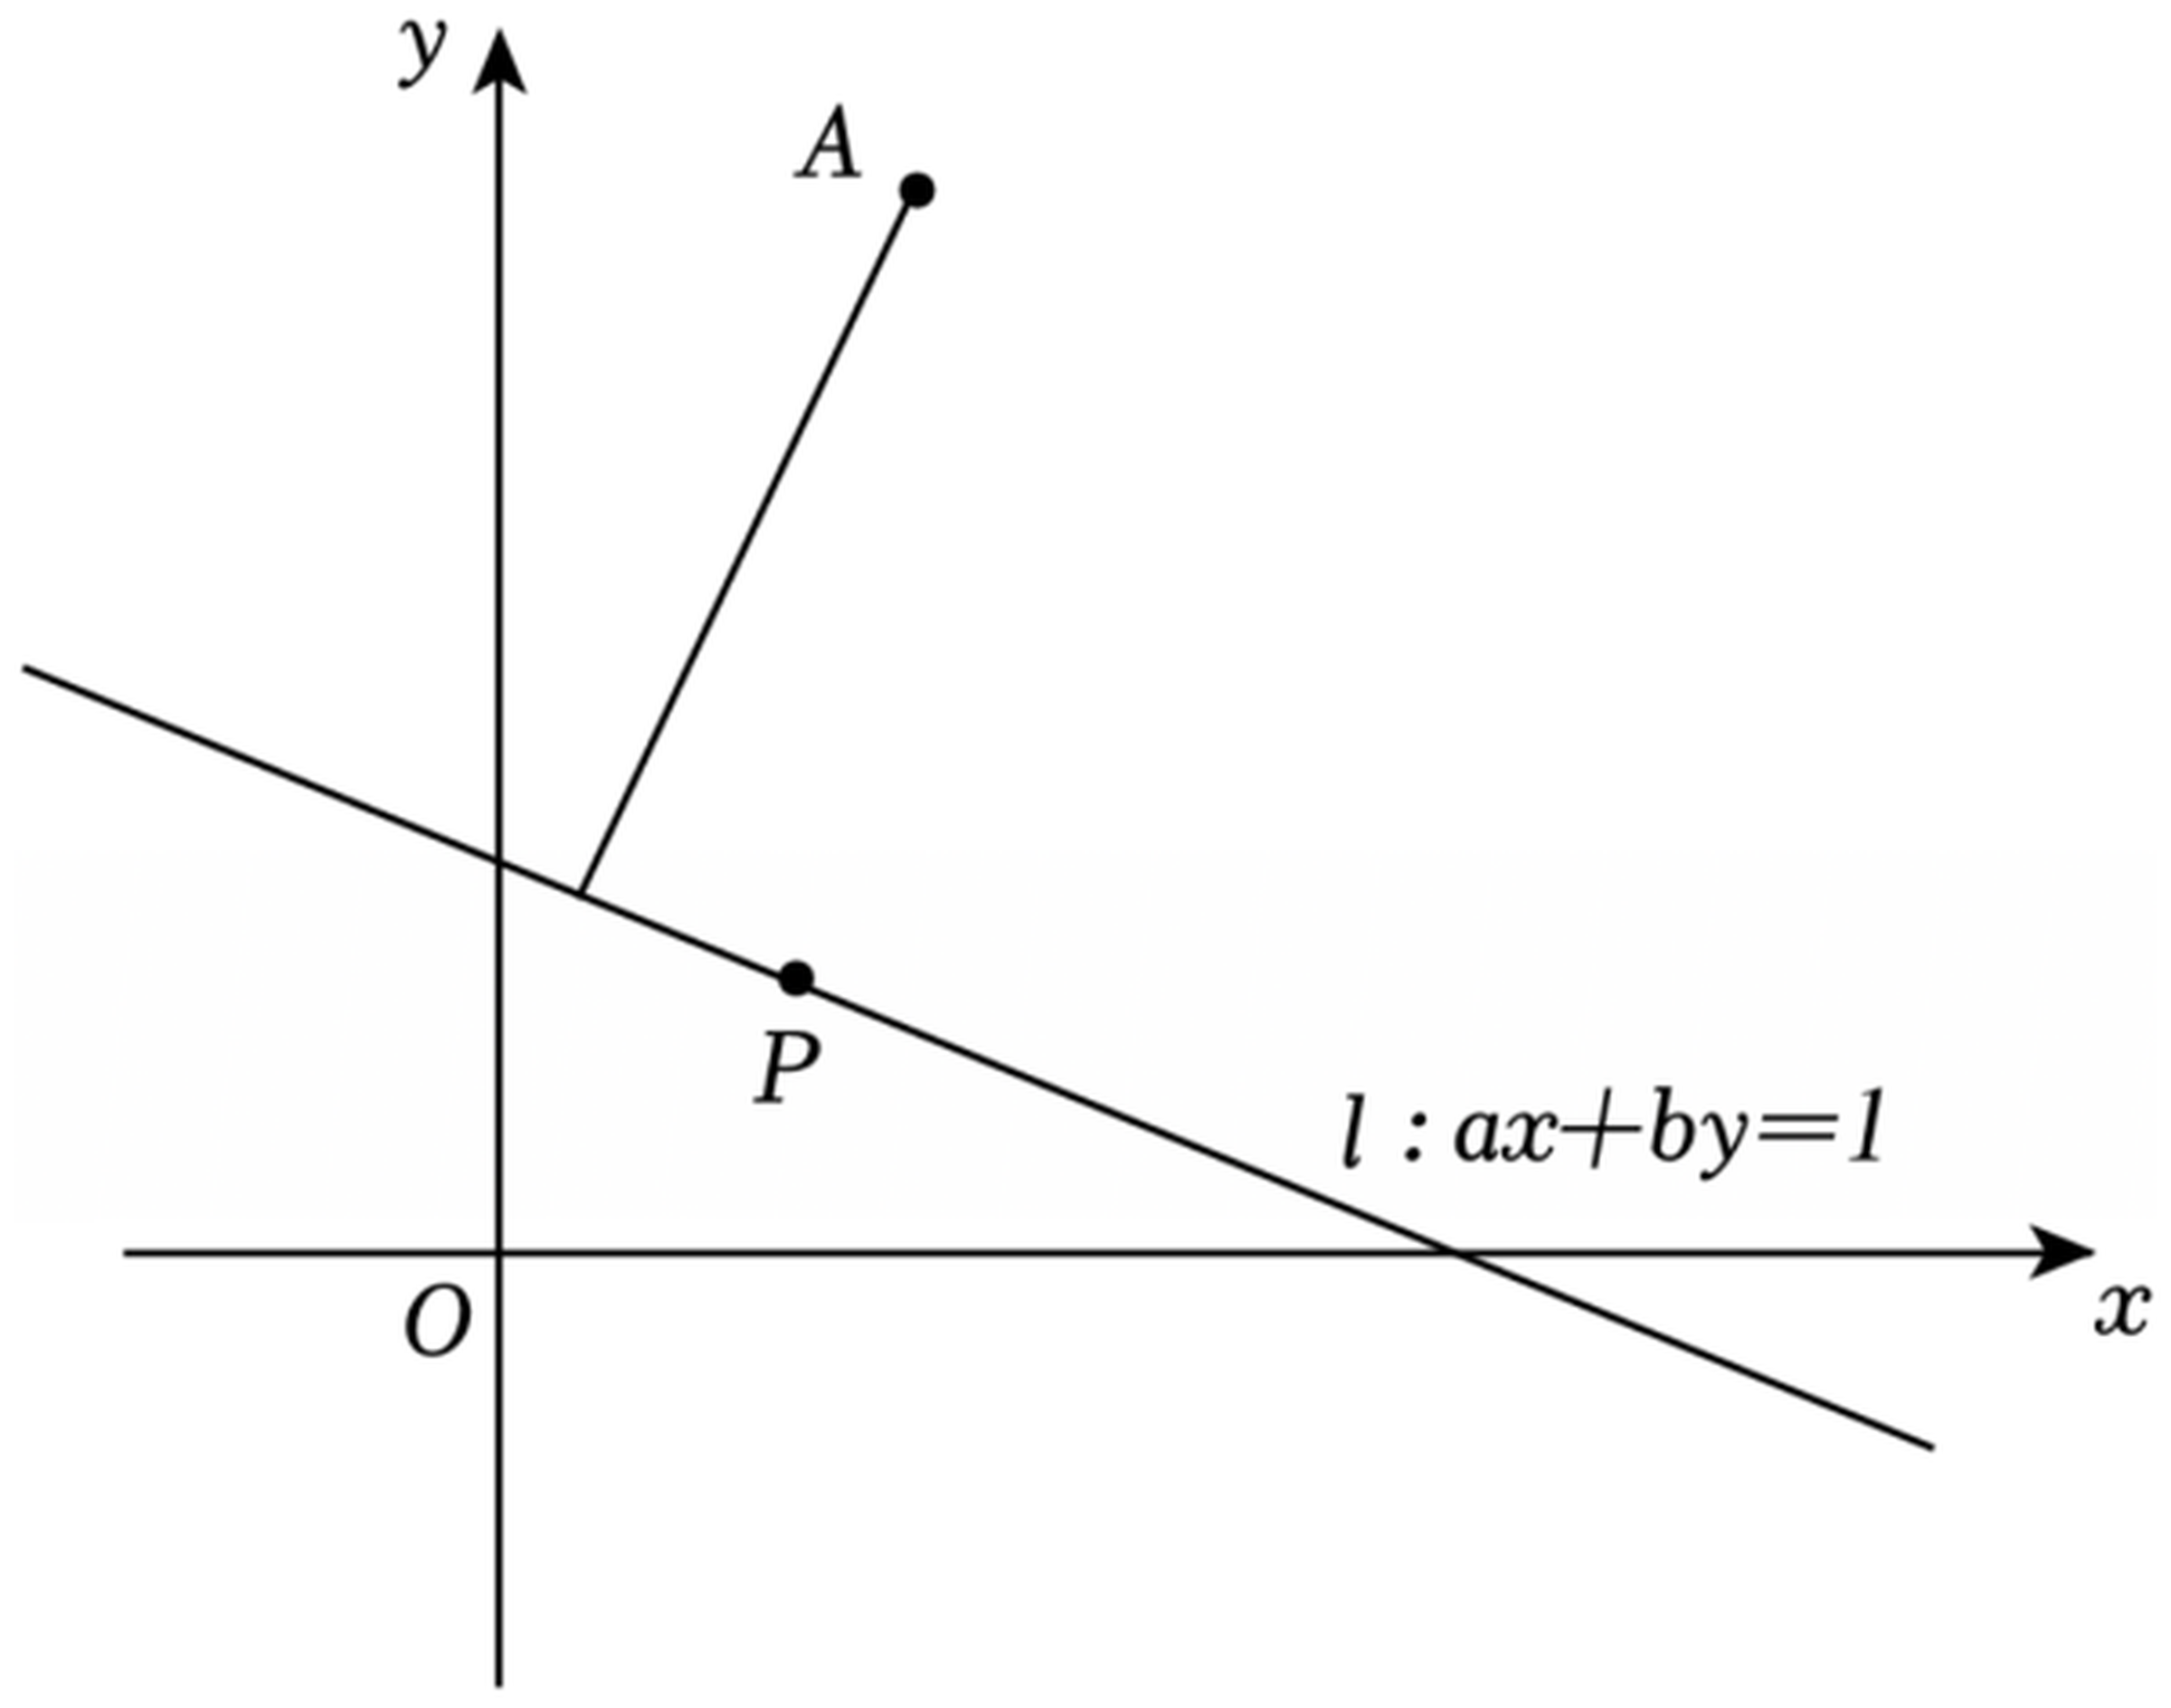
\includegraphics[width=0.56\textwidth]{figures/line_ax_plus_by_1.png}
\end{center}

\step{因为 $a+b=2$，所以直线 $l$ 恒过定点 $P\left(\dfrac12,\dfrac12\right)$，}
\step{再令 $A(1,2)$，则
$d_{A-l}=\dfrac{|a+2b-1|}{\sqrt{a^2+b^2}}\leqslant|AP|=\dfrac{\sqrt{10}}2$，}
\step{当且仅当 $l\perp AP$ 时等号成立，}
\step{又 $\dfrac{a+2b-1}{\sqrt{a^2+b^2}}\leqslant\dfrac{|a+2b-1|}{\sqrt{a^2+b^2}}$，
而当 $l\perp AP$，$a+2b-1>0$，等号也成立，}
\step{故 $\left(\dfrac{a+2b-1}{\sqrt{a^2+b^2}}\right)_{\max}=\dfrac{\sqrt{10}}2$.}
\solend

\fi

\ansspace[6]

\item （1）设 $a$、$b$、$c$ 都是正数，试证明不等式：
$\dfrac{b+c}a+\dfrac{c+a}b+\dfrac{a+b}c\geqslant6$；

（2）对一切正整数 $n$，不等式 $\dfrac{2x-1}x>\dfrac n{n+1}$ 恒成立，
则实数 $x$ 的取值范围构成的集合.

\ifanswer
\solbegin
\stepm{(1)}{因为 $a>0$，$b>0$，$c>0$，}
\step{所以 $\dfrac ba+\dfrac ab\geqslant2$，$\dfrac ca+\dfrac ac\geqslant2$，
$\dfrac cb+\dfrac bc\geqslant2$，}
\step{所以 $\left(\dfrac ba+\dfrac ab\right)+\left(\dfrac ca+\dfrac ac\right)
+\left(\dfrac cb+\dfrac bc\right)\geqslant6$，
即 $\dfrac{b+c}a+\dfrac{c+a}b+\dfrac{a+b}c\geqslant6$.}
% 注：下一行题干原卷作「……则实数 $x$ 的取值范围构成的集合.」，缺一个「求」字，
%     照抄未改，见文件头「原卷存疑」⑤。
\stepm{(2)}{考查 $y=\dfrac n{n+1}=1-\dfrac1{n+1}$，一切正整数 $n$ 函数为严格增函数，
所以 $y\geqslant\dfrac12$，}
\step{对一切正整数 $n$，不等式 $\dfrac{2x-1}x>\dfrac n{n+1}$ 恒成立，
所以 $\dfrac{2x-1}x\geqslant1$，}
\step{所以 $\dfrac{x-1}x\geqslant0$，所以 $x<0$ 或 $x\geqslant1$，}
\step{所以实数 $x$ 的取值范围是 $(-\infty,0)\cup[1,+\infty)$.}
\solend

\fi

\ansspace[6]

\end{enumerate}

\end{document}
"
%
% 原始材料是微信公众号图文（公众号「魔都数学加油站」连载「27学年高一 34」，2026-09-25 发布，
% 原文标题「27学年高一34——2026-2027年上海市交附闵行高一上查漏补缺卷」），
% 正文为 7 张 PNG 页（均 2560×3620），取 mmbiz.qpic.cn/<hash>/0 的原图档。
% 原文本身就是一份**讲评版**，但**全卷没有任何一处印「【答案】」**——每题下方直接印【解析】，
% 答案写在解析的末句。试题文字与解析均照原卷录入，未改内容。
% 卷面的粉色斜水印属水印，未录入。
%
% 卷首标题：原卷印作「2026-2027 年交附闵行高一上查漏补缺卷」（公众号标题里的「上海市」
% 三字卷面标题行没有，本稿照卷面），年份区间按全稿惯例排 en dash，前缀照原卷保留「年」。
%
% 与原卷的排版差异（均已在 README「说明」中交代）：
%   ① 原文自**第 3 题**起（第 1、2 题未在该文中发布），故本稿题号亦自 3 起；
%   ② 原卷只有「一、填空题」「二、解答题」两个节标题（本卷无选择题），本稿照原卷分节，
%      只把标题改排成全稿统一的「大节标题」样式；
%   ③ 原卷通篇只印【解析】（无【答案】行），本稿统一改为试卷版隐去、答案版以 \ifanswer{}
%      块给出，两版彻底分离；
%   ④ 数集记号原卷两套并用：第 4 题与第 11(2) 题作斜体的 $R$，第 7 题两处作粗体的
%      $\mathbf{R}^+$，本稿按全稿惯例统一写作 $\R$；
%   ⑤ 原卷填空的横线约两个字宽，本稿按全稿惯例统一排 \blankline[4.4em]（第 9 题的第一个空
%      原卷**没有**下划线、只留了一个空格，本稿仍补出横线，见文件头「原卷存疑」①）；
%   ⑥ 原卷未印副标题，本稿按全稿惯例补出副标题「集合与常用逻辑用语」（本卷实为基本不等式
%      专题，与 高一27／高一28 同样只标主章节，见文末「高一34 专记」）；
%   ⑦ 第 13 题的配图只出现在【解析】里（题干并未写「如图」），故放进 \ifanswer 块，
%      试卷版不排；图取原卷截图、4× LANCZOS 放大（figures/line_ax_plus_by_1.png）。
%
% 原卷存疑五处（均照抄原卷、未改，见源码中该处上方注释）：
%   ① 第 9 题「则 $ab$ 的最大值为 ，」——第一个空后面只有空格、没有下划线，第二个空才有；
%   ② 第 11(2) 题题干括号内写「$a$、$b\in R$」，但函数式 $f(x)=ax^2+(3a-4)x-12$ 里并没有 $b$；
%   ③ 第 10 题只限定 $a$ 是正实数，未提 $b$ 的取值范围；
%   ④ 第 13 题题干作「求 …… 的最大值为____.」（「求」与「为」混用），且**题干未写「如图」**，
%      是【解析】里才写「如图」；
%   ⑤ 第 14(2) 题题干作「……则实数 $x$ 的取值范围构成的集合.」——缺一个「求」字。
% 另有两处标点照录：第 9 题【解析】首句末是句号、第 11(1)① 解析末句是分号。

\documentclass[a4paper,11pt]{article}
\usepackage{common}

\begin{document}

\examtitlest[3]{2026--2027 年交附闵行高一上查漏补缺卷}{集合与常用逻辑用语}

\bigsec{一、填空题}

\begin{enumerate}
\setcounter{enumi}{2}

\item 已知正实数 $m$、$n$ 满足 $\dfrac1{m+2n}+\dfrac1{2m+n}=1$，则 $m+n$ 的最小值为
\blankline[4.4em].

\ifanswer
\solbegin
\step{因为 $m$、$n\in(0,+\infty)$，$\dfrac1{m+2n}+\dfrac1{2m+n}=1$，}
\step{所以 $m+n=\dfrac13[(m+2n)+(2m+n)]\left(\dfrac1{m+2n}+\dfrac1{2m+n}\right)$}
\step{$=\dfrac13\left[2+\dfrac{2m+n}{m+2n}+\dfrac{m+2n}{2m+n}\right]
\geqslant\dfrac13\left[2+2\sqrt{\dfrac{2m+n}{m+2n}\cdot\dfrac{m+2n}{2m+n}}\right]
=\dfrac43$，}
\step{当且仅当 $\dfrac{2m+n}{m+2n}=\dfrac{m+2n}{2m+n}$，即 $m=n=\dfrac23$ 时取等号，}
\step{所以 $m+n$ 的最小值为 $\dfrac43$.}
\solend

\fi

\item 若 $a$、$b\in\R$，且 $a^2+2ab-3b^2=1$，则 $a^2+b^2$ 的最小值为 \blankline[4.4em].

\ifanswer
\solbegin
\step{由 $a^2+2ab-3b^2=1$ 得 $(a+3b)(a-b)=1$，}
\step{令 $x=a+3b$，$y=a-b$，则 $xy=1$ 且 $a=\dfrac{x+3y}4$，$b=\dfrac{x-y}4$，}
\step{所以 $a^2+b^2=\left(\dfrac{x+3y}4\right)^2+\left(\dfrac{x-y}4\right)^2
=\dfrac{x^2+5y^2+2}8\geqslant\dfrac{2\sqrt{5x^2y^2}+2}8=\dfrac{\sqrt5+1}4$，}
\step{当且仅当 $x^2=\sqrt5$，$y^2=\dfrac{\sqrt5}5$ 时取等号，
故 $a^2+b^2$ 的最小值为 $\dfrac{\sqrt5+1}4$.}
\solend

\fi

\item 已知实数 $x$、$y$ 满足 $3x^2+3y^2-2xy=4$，则 $x+y$ 的最大值为 \blankline[4.4em].

\ifanswer
\solbegin
\step{由 $3x^2+3y^2-2xy=4$，则 $3[(x+y)^2-2xy]-2xy=4$，}
\step{设 $s=x+y$，则 $3s^2-8xy=4$，即 $xy=\dfrac{3s^2-4}8$，}
\step{对任意实数 $x$、$y$，有 $xy\leqslant\left(\dfrac{x+y}2\right)^2=\dfrac{s^2}4$，
即 $\dfrac{3s^2-4}8\leqslant\dfrac{s^2}4$，}
\step{得 $s^2\leqslant4$，即 $-2\leqslant s\leqslant2$，}
\step{当 $x=y=1$ 时，满足原等式，且 $x+y=2$ 成立，因此 $x+y$ 的最大值为 $2$.}
\solend

\fi

\item 若 $a$、$b$、$c$ 都是正实数，则 $\dfrac{a^2+2b^2+4c^2}{ab+2bc}$ 的最小值为
\blankline[4.4em].

\ifanswer
\solbegin
\step{因为 $a^2+2b^2+4c^2=a^2+b^2+b^2+4c^2=(a^2+b^2)+(b^2+4c^2)\geqslant2ab+4bc$，}
\step{所以 $\dfrac{a^2+2b^2+4c^2}{ab+2bc}\geqslant\dfrac{2ab+4bc}{ab+2bc}=2$，
当且仅当 $a=b=2c$ 时取等号，}
\step{即 $\dfrac{a^2+2b^2+4c^2}{ab+2bc}$ 的最小值是 $2$.}
\solend

\fi

\item 已知 $a$、$b\in\R^+$，且 $ab=2$，则 $\dfrac b{2+a^2}+\dfrac a{2+b^2}$ 的最小值是
\blankline[4.4em].

\ifanswer
\solbegin
\step{$\dfrac b{2+a^2}+\dfrac a{2+b^2}=\dfrac b{ab+a^2}+\dfrac a{ab+b^2}
=\dfrac b{a(a+b)}+\dfrac a{b(a+b)}$}
\step{$=\dfrac{(a+b)^2-4}{2(a+b)}=\dfrac{a+b}2-\dfrac2{a+b}$，}
\step{令 $t=a+b$，则原式可设为 $y=\dfrac t2-\dfrac2t$ 的函数，}
\step{当 $t>0$ 时，此函数为严格增函数，}
\step{因为 $a$、$b\in\R^+$ 且 $ab=2$，$t=a+b\geqslant2\sqrt{ab}=2\sqrt2$，}
\step{当且仅当 $a=b=\sqrt2$ 时，$t$ 的最小值为 $2\sqrt2$，}
\step{$y=\dfrac t2-\dfrac2t$ 在 $t\in[2\sqrt2,+\infty)$ 上严格增，}
\step{所以原式的最小值为 $\dfrac{2\sqrt2}2-\dfrac2{2\sqrt2}=\dfrac{\sqrt2}2$，
则 $\dfrac b{2+a^2}+\dfrac a{2+b^2}$ 的最小值是 $\dfrac{\sqrt2}2$.}
\solend

\fi

\item 设 $x$、$y$、$z$ 为正实数，满足 $x-2y+3z=0$，则 $\dfrac{y^2}{xz}$ 的最小值是
\blankline[4.4em].

\ifanswer
\solbegin
\step{因为 $x-2y+3z=0$，所以 $y=\dfrac{x+3z}2$，}
\step{所以 $\dfrac{y^2}{xz}=\dfrac{x^2+9z^2+6xz}{4xz}\geqslant\dfrac{6xz+6xz}{4xz}=3$，
当且仅当 $x=3z$ 时取等号，}
\step{故 $\dfrac{y^2}{xz}$ 的最小值是 $3$.}
\solend

\fi

% 注：下一题的第一个空原卷只留了一个空格、**没有**下划线（第二个空才有），本稿仍按全稿
%     惯例补出横线；另其【解析】首句末原卷作句号，照录。见文件头「原卷存疑」①。
\item 设 $a$、$b$ 为正实数，且 $a+b=3$，则 $ab$ 的最大值为 \blankline[4.4em]，
$\dfrac{a^2}{a+2}+\dfrac{b^2}{b+1}$ 的最小值为 \blankline[4.4em].

\ifanswer
\solbegin
\step{因为 $a>0$，$b>0$，所以 $a+b=3\geqslant2\sqrt{ab}$，}
\step{故 $ab$ 的最大值为 $\dfrac94$，当且仅当 $a=b=\dfrac32$ 时取等号.}
\step{令 $a+2=m$，$b+1=n$，则 $m+n=a+b+3=6$，}
\step{解得 $a=m-2$，$b=n-1$，}
\step{所以 $\dfrac{a^2}{a+2}+\dfrac{b^2}{b+1}=\dfrac{(m-2)^2}m+\dfrac{(n-1)^2}n
=m+\dfrac4m+n+\dfrac1n-6=\dfrac4m+\dfrac1n$}
\step{$=\dfrac16(m+n)\left(\dfrac4m+\dfrac1n\right)
=\dfrac16\left(\dfrac{4n}m+\dfrac mn+5\right)\geqslant\dfrac16(4+5)=\dfrac32$，}
\step{当且仅当 $\dfrac{4n}m=\dfrac mn$ 时，即 $m=2n$ 时
$\dfrac{a^2}{a+2}+\dfrac{b^2}{b+1}$ 取得最小值，}
\step{因此 $\dfrac{a^2}{a+2}+\dfrac{b^2}{b+1}$ 的最小值为 $\dfrac32$.}
\solend

\fi

\item 若 $a$ 是正实数，$2a^2+3b^2=10$，则 $a\sqrt{2+b^2}$ 的最大值是 \blankline[4.4em].

\ifanswer
\solbegin
\step{$a$ 是正实数，$2a^2+3b^2=10$，变形为 $2a^2+3(b^2+2)=16$，}
\step{所以 $16\geqslant2\sqrt{2a^2\times3(b^2+2)}=2\sqrt6\cdot a\sqrt{b^2+2}$，
得 $a\sqrt{2+b^2}\leqslant\dfrac{4\sqrt6}3$，}
\step{当且仅当 $2a^2=3(b^2+2)=8$，即 $a=2$，$b^2=\dfrac23$ 时取等号，}
\step{所以 $a\sqrt{2+b^2}$ 的最大值为 $\dfrac{4\sqrt6}3$.}
\solend

\fi

\end{enumerate}

\bigsec{二、解答题}

\begin{enumerate}
\setcounter{enumi}{10}

\item （1）已知 $x>0$，$y>0$，$2xy=x+4y$. ①求 $xy$ 的最小值；②求 $x+y$ 的最小值.

（2）已知函数 $f(x)=ax^2+(3a-4)x-12$（$a$、$b\in\R$），求不等式 $f(x)\geqslant0$ 的解集.

\ifanswer
\solbegin
\stepm{(1)}{①因为 $x>0$，$y>0$，由基本不等式得
$2xy=x+4y\geqslant2\sqrt{4xy}=4\sqrt{xy}$，}
\step{解得 $xy\geqslant4$，当且仅当 $x=4y=4$ 时取等号，故 $xy$ 的最小值为 $4$；}
\step{②因为 $x>0$，$y>0$，由已知条件得 $\dfrac{4y+x}{xy}=\dfrac4x+\dfrac1y=2$，}
\step{所以 $x+y=\dfrac12(x+y)\left(\dfrac4x+\dfrac1y\right)
=\dfrac12\left(5+\dfrac{4y}x+\dfrac xy\right)
\geqslant\dfrac12\left(5+2\sqrt{\dfrac{4y}x\cdot\dfrac xy}\right)=\dfrac92$，}
\step{当且仅当 $x=2y=3$ 时，等号成立，故 $x+y$ 的最小值为 $\dfrac92$；}
% 注：下一行题干括号内原卷写「$a$、$b\in R$」，但函数式里并没有 $b$，照抄未改，
%     见文件头「原卷存疑」②。
\stepm{(2)}{当 $a=0$ 时，则 $x+3\leqslant0$，解得 $x\leqslant-3$；}
\step{当 $a\neq0$ 时，$f(x)=ax^2+(3a-4)x-12=(x+3)(ax-4)
=a(x+3)\left(x-\dfrac4a\right)$，}
\step{当 $a>0$ 时，则 $(x+3)\left(x-\dfrac4a\right)\geqslant0$，
解得 $x\leqslant-3$ 或 $x\geqslant\dfrac4a$；}
\step{当 $a<0$ 时，则 $(x+3)\left(x-\dfrac4a\right)\leqslant0$，}
\step{当 $\dfrac4a>-3$ 时，即 $a<-\dfrac43$，解 $(x+3)\left(x-\dfrac4a\right)\leqslant0$，
得 $-3\leqslant x\leqslant\dfrac4a$；}
\step{当 $\dfrac4a=-3$ 时，即 $a=-\dfrac43$，解 $(x+3)\left(x-\dfrac4a\right)\leqslant0$，
得 $x=-3$；}
\step{当 $\dfrac4a<-3$ 时，即 $-\dfrac43<a<0$，解 $(x+3)\left(x-\dfrac4a\right)\leqslant0$，
得 $\dfrac4a\leqslant x\leqslant-3$；}
\step{综上所述，当 $a<-\dfrac43$ 时，不等式 $f(x)\geqslant0$ 的解集为
$\left[-3,\dfrac4a\right]$；}
\step{当 $a=-\dfrac43$ 时，不等式 $f(x)\geqslant0$ 的解集为 $\{-3\}$；}
\step{当 $-\dfrac43<a<0$ 时，不等式 $f(x)\geqslant0$ 的解集为
$\left[\dfrac4a,-3\right]$；}
\step{当 $a=0$ 时，不等式 $f(x)\geqslant0$ 的解集为 $(-\infty,-3]$；}
\step{当 $a>0$ 时，不等式 $f(x)\geqslant0$ 的解集为
$(-\infty,-3]\cup\left[\dfrac4a,+\infty\right)$.}
\solend

\fi

\ansspace[8]

\item 已知 $x$、$y$ 都是正数，且 $\dfrac2x+\dfrac1y=1$.

\begin{enumerate}[label=(\arabic*)]
\item 求 $2x+y$ 的最小值及此时 $x$、$y$ 的取值；
\item 不等式 $(2x+y)^2\geqslant m(x+2y)$ 恒成立，求实数 $m$ 的取值范围.
\end{enumerate}

\ifanswer
\solbegin
\stepm{(1)}{$2x+y=(2x+y)\left(\dfrac2x+\dfrac1y\right)
=4+\dfrac{2x}y+\dfrac{2y}x+1\geqslant5+2\sqrt{\dfrac{2x}y\cdot\dfrac{2y}x}=9$，}
\step{当且仅当 $x=y$ 且 $\dfrac2x+\dfrac1y=1$，即 $x=y=3$ 时取等号，}
\step{此时 $2x+y$ 的最小值为 $9$.}
\stepm{(2)}{由 $\dfrac2x+\dfrac1y=1$，得 $x+2y=xy>0$，}
\step{故 $(2x+y)^2\geqslant m(x+2y)\Leftrightarrow m\leqslant\dfrac{(2x+y)^2}{x+2y}
\Leftrightarrow m\leqslant\dfrac{(2x+y)^2}{xy}$，}
\step{又 $\dfrac{(2x+y)^2}{xy}=\dfrac{4x^2+y^2+4xy}{xy}
=\dfrac{4x}y+\dfrac yx+4\geqslant2\sqrt{\dfrac{4x}y\cdot\dfrac yx}+4=8$，}
\step{当且仅当 $\begin{cases}\dfrac{4x}y=\dfrac yx\\[2pt]
\dfrac2x+\dfrac1y=1\end{cases}$ 时取等号，$\dfrac{(2x+y)^2}{xy}$ 取得最小值 $8$，}
\step{故 $m$ 的取值范围为 $\{m\mid m\leqslant8\}$.}
\solend

\fi

\ansspace[6]

% 注：本小题题干作「求 …… 的最大值为____.」（「求」与「为」混用），且**题干未写「如图」**
%     ——是【解析】里才写「如图」，照抄未改，见文件头「原卷存疑」④。
\item 已知实数 $a$、$b$ 满足 $a+b=2$，求 $\dfrac{a+2b-1}{\sqrt{a^2+b^2}}$ 的最大值为
\blankline[4.4em].

\ifanswer
\solbegin
\step{如图，考虑直线 $l:ax+by=1$，}

\begin{center}
% 图取原卷截图、4× LANCZOS 放大。图只在【解析】里出现（题干并未写「如图」），
% 故放进 \ifanswer 块，试卷版不排，见文件头⑦。
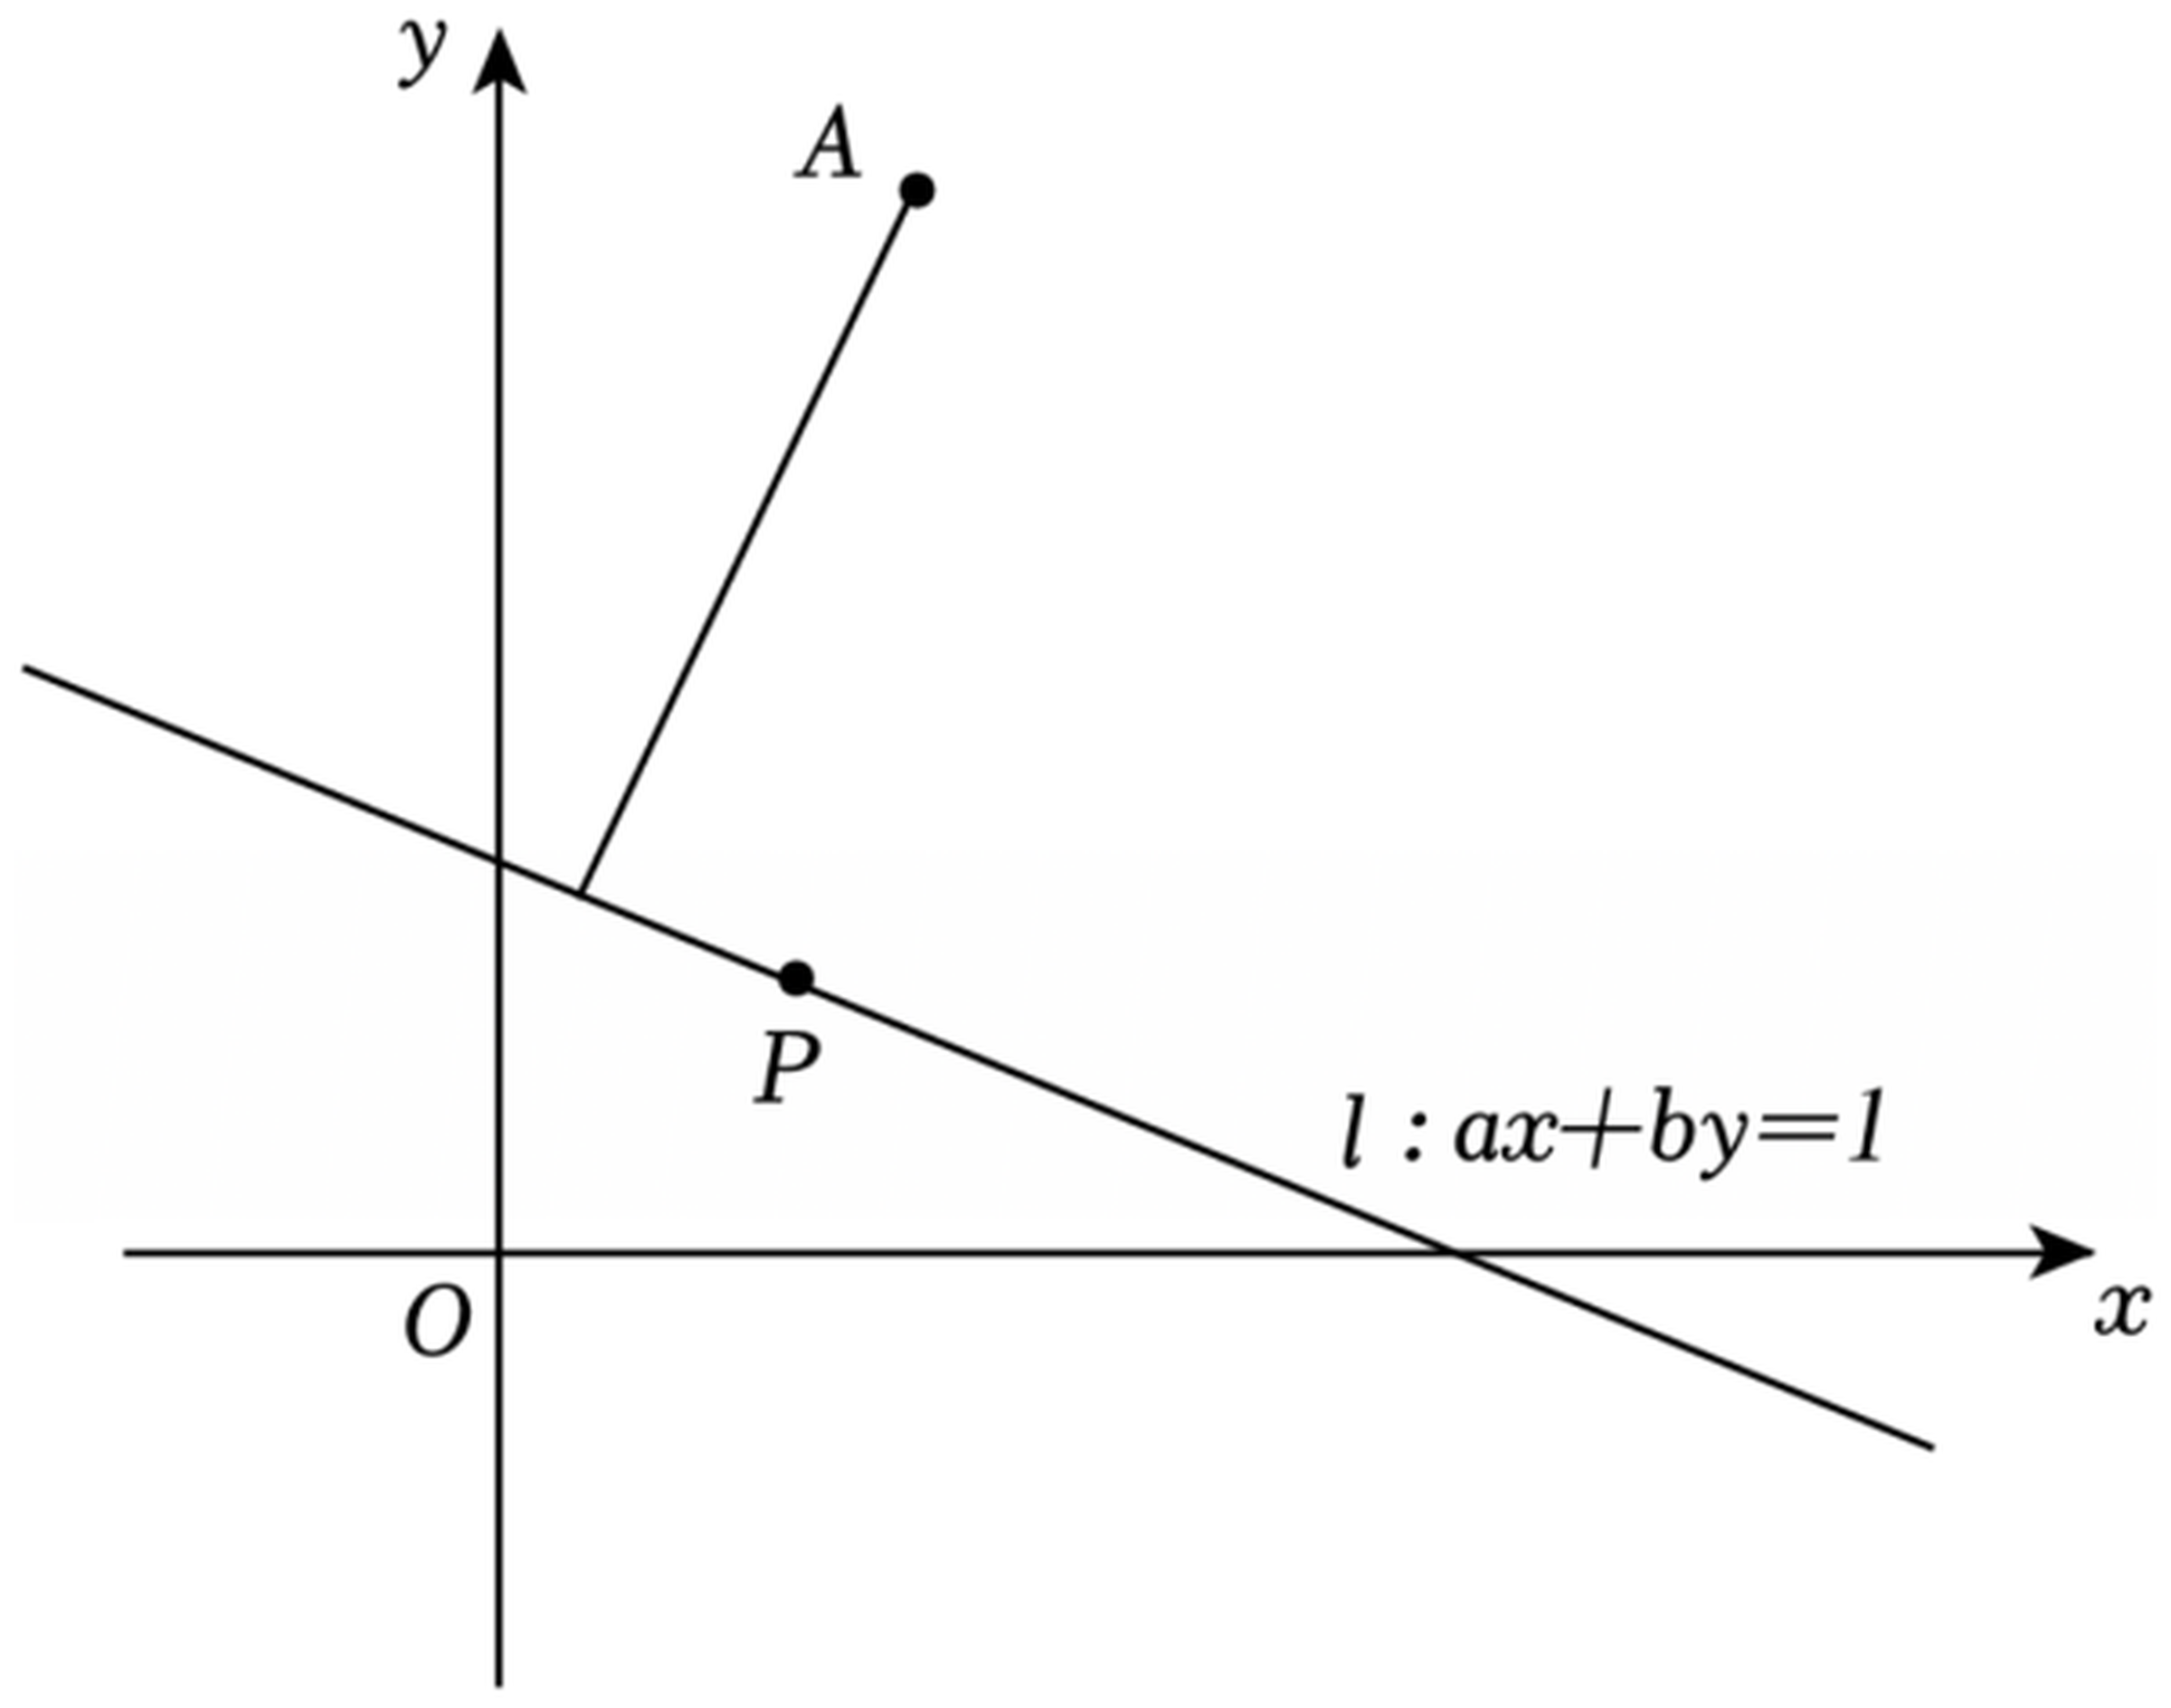
\includegraphics[width=0.56\textwidth]{figures/line_ax_plus_by_1.png}
\end{center}

\step{因为 $a+b=2$，所以直线 $l$ 恒过定点 $P\left(\dfrac12,\dfrac12\right)$，}
\step{再令 $A(1,2)$，则
$d_{A-l}=\dfrac{|a+2b-1|}{\sqrt{a^2+b^2}}\leqslant|AP|=\dfrac{\sqrt{10}}2$，}
\step{当且仅当 $l\perp AP$ 时等号成立，}
\step{又 $\dfrac{a+2b-1}{\sqrt{a^2+b^2}}\leqslant\dfrac{|a+2b-1|}{\sqrt{a^2+b^2}}$，
而当 $l\perp AP$，$a+2b-1>0$，等号也成立，}
\step{故 $\left(\dfrac{a+2b-1}{\sqrt{a^2+b^2}}\right)_{\max}=\dfrac{\sqrt{10}}2$.}
\solend

\fi

\ansspace[6]

\item （1）设 $a$、$b$、$c$ 都是正数，试证明不等式：
$\dfrac{b+c}a+\dfrac{c+a}b+\dfrac{a+b}c\geqslant6$；

（2）对一切正整数 $n$，不等式 $\dfrac{2x-1}x>\dfrac n{n+1}$ 恒成立，
则实数 $x$ 的取值范围构成的集合.

\ifanswer
\solbegin
\stepm{(1)}{因为 $a>0$，$b>0$，$c>0$，}
\step{所以 $\dfrac ba+\dfrac ab\geqslant2$，$\dfrac ca+\dfrac ac\geqslant2$，
$\dfrac cb+\dfrac bc\geqslant2$，}
\step{所以 $\left(\dfrac ba+\dfrac ab\right)+\left(\dfrac ca+\dfrac ac\right)
+\left(\dfrac cb+\dfrac bc\right)\geqslant6$，
即 $\dfrac{b+c}a+\dfrac{c+a}b+\dfrac{a+b}c\geqslant6$.}
% 注：下一行题干原卷作「……则实数 $x$ 的取值范围构成的集合.」，缺一个「求」字，
%     照抄未改，见文件头「原卷存疑」⑤。
\stepm{(2)}{考查 $y=\dfrac n{n+1}=1-\dfrac1{n+1}$，一切正整数 $n$ 函数为严格增函数，
所以 $y\geqslant\dfrac12$，}
\step{对一切正整数 $n$，不等式 $\dfrac{2x-1}x>\dfrac n{n+1}$ 恒成立，
所以 $\dfrac{2x-1}x\geqslant1$，}
\step{所以 $\dfrac{x-1}x\geqslant0$，所以 $x<0$ 或 $x\geqslant1$，}
\step{所以实数 $x$ 的取值范围是 $(-\infty,0)\cup[1,+\infty)$.}
\solend

\fi

\ansspace[6]

\end{enumerate}

\end{document}
